%  ========================================================================
%  Copyright (c) 1985 The University of Washington
%
%  Licensed under the Apache License, Version 2.0 (the "License");
%  you may not use this file except in compliance with the License.
%  You may obtain a copy of the License at
%
%      http://www.apache.org/licenses/LICENSE-2.0
%
%  Unless required by applicable law or agreed to in writing, software
%  distributed under the License is distributed on an "AS IS" BASIS,
%  WITHOUT WARRANTIES OR CONDITIONS OF ANY KIND, either express or implied.
%  See the License for the specific language governing permissions and
%  limitations under the License.
%  ========================================================================
%

% Documentation for University of Washington thesis LaTeX document class
% by Jim Fox
% fox@washington.edu
%
%    Revised 2020/02/24, added \caption()[]{} option.  No ToC.
%
%    Revised for version 2015/03/03 of uwthesis.cls
%    Revised, 2016/11/22, for cleanup of sample copyright and title pages
%
%    This document is contained in a single file ONLY because
%    I wanted to be able to distribute it easily.  A real thesis ought
%    to be contained on many files (e.g., one for each chapter, at least).
%
%    To help you identify the files and sections in this large file
%    I use the string '==========' to identify new files.
%
%    To help you ignore the unusual things I do with this sample document
%    I try to use the notation
%       
%    % --- sample stuff only -----
%    special stuff for my document, but you don't need it in your thesis
%    % --- end-of-sample-stuff ---


%    Printed in twoside style now that that's allowed
%
 
\documentclass [11pt, proquest] {uwthesis}[2020/02/24]
 
%
% The following line would print the thesis in a postscript font 

% \usepackage{natbib}
% \def\bibpreamble{\protect\addcontentsline{toc}{chapter}{Bibliography}}

\setcounter{tocdepth}{1}  % Print the chapter and sections to the toc
 

% ==========   Local defs and mods
%

% --- sample stuff only -----
% These format the sample code in this document

\usepackage{alltt}  % 
\newenvironment{demo}
  {\begin{alltt}\leftskip3em
     \def\\{\ttfamily\char`\\}%
     \def\{{\ttfamily\char`\{}%
     \def\}{\ttfamily\char`\}}}
  {\end{alltt}}
 
% metafont font.  If logo not available, use the second form
%
% \font\mffont=logosl10 scaled\magstep1
\let\mffont=\sf
% --- end-of-sample-stuff ---
 

\usepackage{amsmath}
\usepackage{amssymb}
\usepackage{amsthm}
\usepackage{amsfonts}
\usepackage{mathrsfs}
\usepackage{mathtools}

\usepackage{hyperref}
\usepackage{adjustbox}


%% MATH MACROS
\newcommand{\bbF}{\mathbb{F}}
\newcommand{\bbN}{\mathbb{N}}
\newcommand{\bbQ}{\mathbb{Q}}
\newcommand{\bbR}{\mathbb{R}}
\newcommand{\bbZ}{\mathbb{Z}}
\newcommand{\bbC}{\mathbb{C}}
\newcommand{\Prob}{\mathbb{P}}
\newcommand{\calF}{\mathcal{F}}
\newcommand{\abs}[1]{ \left| #1 \right| }
\newcommand{\diff}[2]{\frac{d #1}{d #2}}
\newcommand{\infsum}[1]{\sum_{#1}^{\infty}}
\newcommand{\norm}[1]{ \left|\left| #1 \right|\right| }
\newcommand{\eval}[1]{ \left. #1 \right| }
\newcommand{\Expect}{\mathbb{E}}
\newcommand{\Var}{\text{Var}}
% \newcommand{\Var}{\mathbb{V}}
\newcommand{\Cov}{\text{Cov}}
\newcommand{\Cor}{\text{Cor}}
\newcommand{\Pois}{\text{Poisson}}
\newcommand{\Binom}{\text{Binomial}}
\newcommand{\Bern}{\text{Bernoulli}}
\newcommand{\Beta}{\text{Beta}}
\newcommand{\Ind}{\mathbf{1}}
\DeclareMathOperator*{\argmin}{arg\,min}
\newcommand{\wt}{W}
\newcommand{\var}{\text{var}}
\newcommand{\varE}{E}
\newcommand{\varT}{T}
\newcommand{\varEscape}{\eta}
\newcommand{\varTransmission}{\rho}
\newcommand{\vac}{\text{vac}}
\newcommand{\evofr}{\texttt{evofr}}
\newcommand{\forecastsNcov}{\texttt{forecasts-ncov}}

\renewcommand{\phi}{\varphi}
\renewcommand{\emptyset}{\O}
\renewcommand{\vec}[1] {\boldsymbol{\mathbf{#1}}}
% \includeonly{chapters/introduction}
\begin{document}
 
% ==========   Preliminary pages
%
% ( revised 2012 for electronic submission )
%

\prelimpages
 
%
% ----- copyright and title pages
%
% \Title{Epidemic-Evolutionary Methods for Evolutionary Forecasting of SARS-CoV-2}
% \Title{Towards Mechanism-informed Evolutionary Forecasting of SARS-CoV-2}
\Title{From Mechanism to Practice: Evolutionary Forecasting for SARS-CoV-2}
\Author{Marlin Figgins}
\Year{2024}
\Program{Applied Mathematics}

\Chair{Ivana Bozic}{Associate Professor}{Applied Mathematics}
\Signature{Trevor Bedford, Advisor}
% \Signature{Erik Matsen}
\Signature{Mark Kot}
% \Signature{Betz Hollaran, GSR}

\copyrightpage

\titlepage  

%
% ----- abstract
%


\setcounter{page}{-1}
\abstract{%

Novel genetic variants often arise due to mutations in circulating viral populations. 
These mutations can sometimes provide fitness advantages to members of the population allowing them to out-compete other variants through mechanisms such as partial immune escape and increased transmissibility.
This interplay of mutation, transmission, and selection leads to evolution in the population.
Therefore, understanding the genetic composition of viral populations and its relation to virus phenotype can be useful for understanding the current and future epidemic potential of viral variants.

This dissertation develops several theoretical ideas, statistical methods, and software tools that enable evolutionary forecasting for SARS-CoV-2 and other rapidly evolving pathogens using concepts from population genetics, mathematical epidemiology, and statistics.

We begin by developing a Bayesian method for estimating the effective reproduction number of genetic variants using counts of variant sequences and measures of incidence such as case counts.

To evaluate this method among others, we develop a workflow to compare frequency-based forecast models in a live forecasting environment, quantifying the short-term accuracy of such methods and suggesting a minimal sequencing capacity to ensure high quality forecasts.

Next, we develop a larger theory for how mechanistic models of transmission constrain how variant frequencies change over time.
This leads to theoretical results for the trade-off between immune escape and increased transmissibility and suggests new methods for modeling variant fitness using approximate Gaussian processes as well as latent pseudo-immune factors.

We then apply these ideas to incorporate molecular data on immune escape and phylogenetic structure into relative fitness estimates to enable out-of-sample prediction of relative fitness from sequence-level predictors.

Our focus then shifts to the operational problem of evolutionary forecasting, where we develop open-source software and visualization tools that can be used to implement, automate, and interpret evolutionary forecasts.

}
 
%
% ----- contents & etc.
%
\tableofcontents
\listoffigures
\listoftables
 
%
% ----- glossary 
%
% \chapter*{Glossary}      % starred form omits the `chapter x'
% \addcontentsline{toc}{chapter}{Glossary}
% \thispagestyle{plain}
% %
% \begin{glossary}
% \item[argument] replacement text which customizes a \LaTeX\ macro for
% each particular usage.
% \item[back-up] a copy of a file to be used when catastrophe strikes
% the original.  People who make no back-ups deserve
% no sympathy.
% \item[control sequence] the normal form of a command to \LaTeX.
% \item[delimiter] something, often a character, that indicates
% the beginning and ending of an argument.
% More generally, a delimiter is a field separator.
% \item[document class] a file of macros that tailors \LaTeX\ for
% a particular document.  The macros described by this thesis
% constitute a document class.
% \item[document option] a macro or file of macros
% that further modifies \LaTeX\ for
% a particular document.  The option {\tt[chapternotes]}
% constitutes a document option.
% \item[figure] illustrated material, including graphs,
% diagrams, drawings and photographs.
% \item[font] a character set (the alphabet plus digits
% and special symbols) of a particular size and style.  A couple of fonts
% used in this thesis are twelve point roman and {\sl twelve point roman
% slanted}.
% \item[footnote] a note placed at the bottom of a page, end of a chapter,
% or end of a thesis that comments on or cites a reference
% for a designated part of the text.
% \item[formatter] (as opposed to a word-processor) arranges printed
% material according to instructions embedded in the text.
% A word-processor, on the other hand, is normally controlled
% by keyboard strokes that move text about on a display.
% \item[\LaTeX] simply the ultimate in computerized typesetting.
% \item[macro]  a complex control sequence composed of 
% other control sequences.
% \item[pica] an archaic unit of length.  One pica is twelve points and
% six picas is about an inch.
% \item[point] a unit of length.  72.27 points equals one inch.
% \item[roman]  a conventional printing typestyle using serifs.
% the decorations on the ends of letter strokes.
% This thesis is set in roman type.
% \item[rule] a straight printed line; e.g., \hrulefill.
% \item[serif] the decoration at the ends of letter strokes.
% \item[table] information placed in a columnar arrangement.
% \item[thesis] either a master's thesis or a doctoral dissertation.
% This document also refers to itself as a thesis, although it
% really is not one.
%  
% \end{glossary}
%  
% %
% ----- acknowledgments
%
\acknowledgments{% \vskip2pc
  % {\narrower\noindent

  I would like to begin by thanking my family, friends, lab members, and other collaborators.
  None of this work would be possible without your patience, kindness, compassion, and collaboration.
  Science cannot be done in isolation.
  This work is the sum of all of our efforts.

  I would like to thank my PhD advisor Trevor Bedford.
  His guidance and belief in me and my work has allowed us to do science that I can be truly proud of.
  His dedication to ensuring that I maintained academic freedom and his encouragement to pursue science that is impactful and practical has completely changed my vision as a scientist, and I am eternally grateful for this.

  I would also like to thank the rest of my committee members: Ivana Bozic, Mark Kot, Erick Matsen, and Betz Halloran.
  Your scientific input and expertise has allowed me to see so many approaches and philosophies of science.
  I could not be writing this without your support and inspiration.

  To all the members of the Bedford lab, thank you for providing a scientific home.
  Though I may not use the words often, you are special to me and I'm honored to work alongside you all.
  Your collective brilliance inspires me daily.

  TEST
  % \par}
}

%
% ----- dedication
%
\dedication{\begin{center} To our best efforts, to our failures, to our successes however marginal.\end{center}}

%
% end of the preliminary pages
 
 
 
%
% ==========      Text pages
%

\textpages
 
% ========== Chapter 1

\chapter{Introduction}

The emergence of SARS-CoV-2, the virus behind COVID-19, has drastically changed our world, affecting health, economies, and daily life. 
First identified in late 2019, this virus quickly spread globally, triggering a pandemic that has impacted millions.

The pandemic had been characterized by recurrent waves of infection, driven by genetic variants such as the Alpha, Beta, Delta, and Omicron variants. \cite{tegally2021detection, Volz2021, vohringer2021genomic, Earnest2021}

Even following the end of the pandemic, there have been multiple infection waves caused by seasonality in transmission as well as evolution of novel SARS-CoV-2 variants that can evade existing immune responses in individuals with past exposure. 

Immune escape driven by antigenic evolution has motivated annual updates to the COVID-19 vaccine to better protect individuals with weakened immune systems and those without past or recent exposure.

Evolution in SARS-CoV-2 has produced genetic variants that exhibit strain-specific immune responses in humans as measured through serology, neutralization titers, and deep mutational scanning assays. \cite{Bekliz2024, Jian2023, Dadonaite2023, Voss2024}

Therefore, understanding both the virus's evolution and transmission dynamics are crucial for managing the pandemic and crafting effective public health strategies.
As SARS-CoV-2 continues to spread, the virus will mutate and new variants with unique traits emerge, influencing their transmissibility, severity, and ability to evade immunity.
% This constantly shifting landscape underscores the importance of forecasting the emergence and spread of these viral variants.

Novel genetic variants often arise due to mutations in currently circulating virus populations.
These mutations can sometimes provide fitness advantages to members of the population allowing them to out-compete other variants through mechanisms such as partial immune escape, increased transmissibility, among others.
This interplay of mutation, transmission, and selection leads to evolution in the population.
Therefore, understanding the genetic composition of viral populations and its relation to virus phenotype can be useful for understanding the current and future epidemic potential of viral variants.

Forecasting these variants is essential for predicting future infection waves, guiding public health measures, and informing vaccine development.
However, this task is challenging due to the virus's rapid mutation rate and the dynamic nature of human immunity and behavior. 

Accurate models are needed to predict how these variants will evolve and spread, to monitor SARS-CoV-2 evolution, and to mitigate future outbreaks.

%TODO: Though SARS-CoV-2 is the primary focus of this dissertation. These methods should generalize.

\paragraph{Objectives and problem statement}

The primary objective of this dissertation is to develop and evaluate models that accurately forecast the evolution and spread of SARS-CoV-2 variants. This involves integrating concepts from epidemiology, evolutionary biology, and applied mathematics to create a comprehensive framework for understanding viral dynamics.

One of the fundamental challenges in forecasting SARS-CoV-2 variants is accounting for the virus's rapid mutation rate and its interaction with the human immune system. Mutations can lead to new variants with increased transmissibility or the ability to evade immunity. To address this, it is essential to incorporate mathematical models that can capture the complexities of viral evolution and spread.

In order to contextualize this work, I will begin with an overview of existing methods for understanding infectious disease transmission, relevant epidemiological quantities, and their relationships to one another.

%TODO: Extend this section, we really also want to menion effective population size, genetic drift .etc
I will then discuss existing methods for understanding population turnover from population genetics and their relationship to some of the related quantities in the epidemiological context.

I will then provide an overview of Bayesian inference, model development, and optimization methods that will be used throughout this dissertation to estimate quantities from data and make predictions while quantifying uncertainty.

Lastly, I will end this introduction by discussing the larger problem of evolutionary forecasting: its components, its aims, and the benefits of developing data-driven evolutionary forecasts on a global scale.
%TODO: This should really end with a description of my contributions.

% My interest is in modeling the epidemic and evolutionary dynamics of virus transmission jointly to better understand how and why virus populations change over time and the consequences of this on human health.
%
% Ultimately, I would like to assess the potential for joint epidemic and evolutionary models to forecast the genetic composition of virus population in the future.
% This may be particularly useful for vaccine strain selection for seasonal influenza and SARS-CoV-2.
%
% To start, I will introduce several preliminary mathematical, biological, and statistical concepts and results needed to re-frame these aims as concrete goals.
%
\section{Epidemic models}

I will give a basic introduction of the ordinary differential equation (ODE) formulation of epidemic models.
We begin with the classic SIR model \cite{KermackMcKendrick1927}.

We will assume that there are three types of individuals in the population: susceptible ($S$), infected ($I$), and recovered ($R$). 
Susceptible individuals can become infected, infected individuals eventually recover (or die), and recovered individuals cannot become infected once again. 
This gives us the system of equations
\begin{align}
  \frac{d S}{d t} &= - \beta S I,\\ 
  \frac{d I}{d t} &= \beta S I - \gamma I,\\
  \frac{d R}{d t} &= \gamma I,
\end{align}
where $\beta$ is an effective infectious contact rate, $\gamma$ is a recovery rate. 
This form of the model lends itself to a couple of analyses that will become important as we extend these models to more complicated infection dynamics.

\paragraph{Effective reproduction number}%

An important quantity that is derived from epidemic models is the effective reproduction number $R_t$. 
We can see that when $R_{t} = \beta S(t) / \gamma > 1$, the number of infected individuals will be increasing, i.e., $\frac{dI}{dt} > 0$. 
This effective reproduction $R_{t}$ controls the direction of the epidemic and reflects the average number of secondary infections caused by a single infection.
In the special case where the population is fully susceptible ($S(t) = 1$), this quantity is called the basic reproduction number $R_{0}$, and it is interpreted as the average number of secondary infections caused by a single individual in an otherwise completely susceptible (naive) population.

% \paragraph{Infectious period}
%
% The second analysis answers the question of how long individuals stay infected under this model. One can show that from the point of infection an individuals rate of becoming uninfectious is constant which implies that the total time spent infected follows an exponential distribution with mean $\tau = \frac{1}{\gamma}$.
%
% Using these facts, we can re-write the differential equation for $I$ as
% \begin{align}
%   \frac{dI}{dt} &= \tau^{-1} (R_{t} - 1)I = r(t) I.
% \end{align}
% Recognizing the differential equation above as that of a time-inhomogeneous exponential growth. 
% We notice that the timing of infectiousness and the effective reproduction number jointly determine the exponential growth rate in an epidemic. 
% In particular, this ODE formulation corresponds to the assumption that the timing between these infections has an exponential distribution. 
% This relationship between timing of reproduction and magnitude of reproduction can be shown more generally.
% %TODO: Though there are ways to generalize this exponential distributed infectious period in the ODE framework, we'll opt for the more general age-structured population dynamic approach.
% %TODO: Mention that generation time and R are needed to make sense of (persistence potential of) exponential growth
% %TODO: Show that this is is not generally true.
%
% \paragraph{Relating effective reproduction number and infection timing}%
%
% We'll also consider more explicitly age-structured transmission models such as renewal equation based models.
%
% In these models, we have that incidence follows
% \begin{align}
%   I(t) = R_{t} \int_{0}^{t} I(t-\tau) g(\tau) d\tau,
% \end{align}
% where $g$ is the density of the generation time $G$ i.e. the timing between primary and secondary infections which acts as a form of the relative transmissibility over the course of an infection.
% We can derive the $R_{t}$ from an age structured population with exponential growth rate $r$ and generation time $G$ as
% \begin{align}
%   \frac{1}{R_{t}} &= \int_{\bbR^{+}} e^{-r\tau} g(\tau) d\tau\\
%                   &=\mathcal{L}_{G}(r) = M_{G}(-r),
% \end{align}
% where we've written the above in terms of a Laplace transform $\mathcal{L}_{G}$ or the moment generating function of $M_{G}$ of the generation time.
% This relationship between $r$ and $R$ can be computed in closed form for several distributions such as the exponential and Gamma \cite{Wallinga2006}.
% For general generation times, we can re-write this in terms of the cumulant generating function of $G$ $K_{G}$ to give the following relationship in terms of moments of $G$, $r$, and $R_{t}$
% \begin{align}
%   \log R_{t} = &- K(-r) \approx \Expect[G] r - \Var[G] \frac{r^{2}}{2} + \left( \Var[G]^{3 / 2} \text{Skew}[G]\right) \frac{r^{3}}{6} + o(r^{4}). \label{eq:central_moment_R}
% \end{align}
%
% Here, it becomes clear that timing of infection and infectiousness is important for interpreting exponential growth rates in terms of the ``average'' transmission dynamics or $R_{t}$ in a population.
%
% We can partially remedy this within the ODE approach by using the "chain trick" in which we allow the infectious individual to remain infectious for non-exponentially generated time period by having multiple sequentially-chained infectious compartments with recover rates $n\gamma$, meaning we replace
% \begin{align*}
%   \frac{d I_{1}}{d t}  &= \beta S \sum_{k=1}^{n} I_{k} - \gamma I_{1}\\
%   \frac{d I_{i}}{d t}  &= n\gamma I_{i-1}- n\gamma I_{i}, \quad 2\leq i \leq n\\
%   \frac{d R}{dt} &= n \gamma I_{n}
% \end{align*}
% In this case, the infectious period is $\text{Gamma}(n, n\gamma)$ distributed with mean $\gamma^{-1}$ and variance. This follows as the infectious period is now the sum of $n$ IID $\text{Exp}(n\gamma)$ random variables. 

% Large $n$ required for complicated serial intervals. Is there a timing first approach.

% More complex models. Specifically allowing us to test various mechanisms for transmission

% Computing $R$ and $R_{0}$. Reference next generation matrix approach here?


% Underlying assumptions of these models with respect to timing on infections. Chain trick as remedy here, reference data showing that these serial intervals are non-exponential to satisfy Mark?
% R, Rt, and methods for estimating R from incidence data?

\section{Multistrain models}

We'll now dive further into the evolutionary component of these models. 
In order for evolution to occur, we need a balance of mutation (generating heritable diversity) and selection (differential survival and reproduction based on that diversity).

For the goal of evolutionary forecasting of virus strains, we need to develop a notion of a multistrain model.
These models will describes population with different types of infecting strains whose differences are heritable.
This enables selection for different strains over time.

\paragraph{A two-strain epidemic model}%

We first consider a standard ODE-based model for infectious diseases with multiple variants: an SIR model in which there are a wild-type $\text{wt}$ and a variant $\text{var}$.
We assume that the variant virus can differ in two ways from the wild type: it may differ in innate transmissibility by a factor of $\eta_{T}$, or it may differ in its infectious period by a factor $\eta_{G}$.
This gives us the system of ordinary differential equations
\begin{align}
  \frac{d S}{d t} &= - \beta S I_{\text{wt}} - \beta \eta_{T} S I_{\text{var}},\\
  \frac{d I_{\text{wt}} }{d t} &= \beta S I_{\text{wt}} - \gamma I_{\text{wt}} = r_{\text{wt}}(t) I_{\text{wt}},\\
  \frac{d I_{\text{var}}}{d t} &= \beta \eta_{T} S I_{\text{var}} - \gamma \eta_{G} I_{\text{var}} = r_{\text{var}}(t) I_{\text{var}}.
\end{align}
% \tbc{Similar comment to in the relative fitness mechanisms manuscript. It's really helpful for my understanding to write out $\phi_\text{wt}$ and $\phi_\text{var}$}.
% MF: I tend to agree but I left it this way since we don't actually discuss anything to do with the $\phi$ here
In this model, we now have two different $R_{0}$ values, $R_{0}^{\text{wt}} = \frac{\beta}{\gamma}$ and $R_{0}^{\text{var}} = \frac{\eta_{T}}{\eta_{G}}R_{0}^{\text{wt}}$.
This shows that there is a dependence between transmissibility and the timing of infections.
If $\eta_{T} > \eta_{G}$, the variant will spread faster than the wildtype, leading to increase in the relative proportion of the variant within the population.

Though this model is not appropriate for infectious diseases with non-trivial competition dynamics via strain-specific immunity for example, it gives us an essential result for epidemiological modeling of genetic variants. \cite{Gog2002}


% More precisely, we notice that without specifying $\eta_{G}$, the variant transmission advantage is unidentifiable.

\section{Population genetics, viral fitness, and selection}

As viruses spread from individual to individual, they generate genetic variation through mutation, drift, and selection.
In the context of ordinary differential equations, we've shown that multiple strains can co-circulate and may dominate one another over time.
However, we still need to develop an understanding of how this co-circulation and transmission affects the underlying population's genetic diversity.

When dealing with pathogens with serial replacement, causing large waves of infection, we're primarily interested in selection.
Selection acts as a ``force'' on the genetic diversity of the population favoring particular genetic variants and causing the population to evolve in response to particular environmental pressures.
We'll now define selection and evolution.

\begin{itemize}
  \item \emph{Selection} is the process by which individuals produce more offspring in certain environments.
% \tbc{this would seem more naturally to me as `leave more offspring' rather than `have higher fitness', although I admit these concepts are synonymous. I just don't think of having higher fitness as a `process'
% MF: Agreed this is more clear.
  \item \emph{Evolution} is the change in the genetic composition of the population over time due to selection, genetic drift, and heritable variation.
    % \tbc{Evolution can also occur due to genetic drift}
    % MF: Tried to change this. I think there's a better way to phrase this however
\end{itemize}

Often, we’re interested in not just the presence of selection but its magnitude.
When quantifying selection in population genetics, the selection coefficient or relative fitness are often discussed.
In the following section, we'll introduce both these quantities and their relationship to one another.

Suppose that we have alleles $A$ and $B$ in a population with $x_A$ individuals having allele $A$ and $x_B$ having allele $B$.
We assume that individuals with alleles $A$ and $B$ produce on average $W_A$ and $W_B$ offspring respectively.
These $W_A$ and $W_B$ are the Wrightian fitness of these alleles.
Assuming that the number of offspring has Poisson distribution with means $W_A$ and $W_B$ respectively, we can write the count of offspring with allele $A$ in the next generation $x_A'$ as

\begin{equation}
x_A' \sim \text{Multinomial}\left(N, \frac{W_A x_A}{W_A x_A + W_B x_B}\right),
\end{equation}
where we've fixed the total number of offspring at $N$.
Using this equation, we can write the expected frequency of allele $A$, $p_A = \frac{x_A}{x_A + x_B}$, and its variance as
\begin{align}
  \Expect[p_A'] &= \frac{W_A p_A }{W_A p_A + W_B p_B} = \frac{W_A}{\bar{W}}p_A,\\
  \Var[p_A'] &= \frac{p_A' (1 - p_A')}{N} \label{eq:allele_variance},
\end{align}
where we have defined the mean fitness $\bar{W} = W_A p_A + W_B p_B$.
This provides a baseline for how fitness changes under fitness dynamics.

To measure the magnitude of selection for a particular allele, we can define the selection coefficient $s$ so that the fitness of $A$ is $W_A = (1+s) W_B$ per generation.
Using our earlier derivation, we can write the expected frequency of the allele $A$ assuming selection coefficient $s$ after $n$ generations of length $\tau$ days

\begin{equation}
  p_A(n) = \frac{(1+s)^{n}p_{A}(0)}{(1+s)^{n}p_{A}(0) + (1 - p_{A}(0))}.
\end{equation}

% \tbc{The subscripting feels a little weird here. You've already used subscript to denote the specific allele ie $p_A$. It looks like it's effectively generation count here? But then shouldn't it be $p_n$ and not $p_{n\tau}$? I get that because it's discrete generations you don't want $p(n)$. Maybe just swap the above from $p_A$ to $p$?}

% MF: Changed this to be consistent with the above.

There are alternative ways to quantify selection.
The methods above used the absolute fitness $W_A$ and $W_B$ to derive selection coefficients $s$ in order to quantify selection.
Alternative models focus on exponentially growing populations.
These approaches have been developed for and applied to modeling SARS-CoV-2 variant turnover.
These models often estimate the relative fitness of variants based on changes in variant frequencies.
\emph{Relative fitness} is the relative capacity for individuals to reproduce in a population.
In exponentially growing populations, we can think about this as the difference between the growth rates.
Where absolute fitness tells us expected number of offspring, relative fitness tells us how variants differ in their capacity to spread.

% \tbc{Clarify the difference between absolute fitness $W_A$ and $W_B$ vs relative fitness of these two alleles. It's almost $s$ right, but quite? It should require the absolute term $W_B$ that $W_A = (1+s) W_B$ entails.}
% MF: I do this a bit later by showing how this definition of relative fitness aligns with $s$.
% MF: For now, I've added a better tie in the previous section and leave the comparison of the two methods for a little down the page.

One model in this vein that has gained popularity for analyzing SARS-CoV-2 variant frequencies and estimating relative fitness is multinomial logistic growth (MLR).
Assuming that each variant has a fixed fitness relative to all others, we can derive a model for variant frequencies over time
\begin{align}
f_{v}(t) = \frac{p_{v}\exp(r_{v}t)}{\sum_{u} p_{u} \exp(r_{u}t)},
\end{align}
where $f_{v}$ is the frequency of variant $v$ in the virus population at time $t$.
Here, $r_{v}$ and $p_{v}$ can be thought of as variant-specific growth rates per day and initial prevalence.
Due to the fact that adding a constant to the growth rates does not affect the frequencies, $r_{v}$ is not uniquely identifiable for all variants.
Additionally, we have the constraint that the initial prevalence of each variant must add to one.
Therefore, we often instead work with a model of the form
\begin{align}
f_{v}(t) = \frac{\exp(\lambda_{v} t + \alpha_{v})}{\sum_{u} \exp(\lambda_{u} t + \alpha_{u})},
\end{align}
where we've set some variant as a pivot with $\lambda_{\text{pivot}} = \alpha_{\text{pivot}}=0$.
By choosing to constrain $\lambda_{\text{pivot}}=0$, we make the model the identifiable.
We've also incorporated the logarithm of the initial prevalence $\log p_v$ into the exponential function as $\alpha_v$, mirroring the form of a generalized linear model.
% \tbc{I'm confused by this. What happened to the initial frequencies $p_v$? It got moved inside the exp to become $alpha_v$? Why do it this way?}
% MF: I gets moved inside for computational reasons basically. It's more complicated to estimate the $p_v$ given they sum to 1.
Using these MLR models, the relative fitness of variant $v$ relative to the pivot is often interpreted as being $\lambda_{v}$.

By using the mean generation time $\tau$, we can approximate the relative effective reproduction number of variants as $R_{t}^{v} / R_{t}^{\text{pivot}} = \exp(\lambda_{v}\tau)$, which is equivalent to assuming that the generation time distribution is a point mass at $\tau$.
This approximation allows us to convert our estimated relative fitness $\lambda_v$ from time in days to a per-generation growth advantage.
% \tbc{Can you say more here about conversion between time in generations vs time in days and what this entails in terms of MLR parameter values?}
We can relate this model of relative fitness to our earlier model of selection by noting that we can convert from number of generations $n$ to number of days $t$ using the generation time, $t = n\tau$.
Substituting the above into our model of selection, we compare the selection coefficient $s$ to the relative fitness $\lambda$,

\begin{equation}
(1 + s)^{t / \tau} = \exp(\lambda_v t) \implies \lambda_v \tau = \log{(1 + s)} \approx s.
\end{equation}

This approximation holds for small $s \approx 0$ using a linear approximation of $\log(1+x)$.
This provides a simple relationship between the traditional selection coefficient $s$ used in population genetics and the relative fitness $\lambda$ that we'll use throughout this dissertation.

\section{Bayesian inference}%

For this general project of relating epidemic dynamics and population genetics, we need to take these models and connect them to what is observed or observable for statistical analysis.
In our case, we rely primarily on Bayesian inference methods.
We'll shortly review several features of Bayesian inference that are useful for this kind of modeling.

In short, Bayesian inference is focused on the properties of the joint probability distribution  $p(\vec{x}, \vec{\theta})$ of data $\vec{x}$ and parameters $\vec{\theta}$ under a given model $m$.

\paragraph{Posterior distribution.}
Given a model and data, we can provide estimates of a possible distribution of parameters conditional on observed data using Bayes rule
\begin{align}
p(\vec{\theta} \mid \vec{x}) = \frac{p(\vec{x} \mid \vec{\theta})\cdot p(\vec{\theta})}{\int p(\vec{x} \mid \vec{\theta}') p(\vec{\theta}') d \vec{\theta}'}.
\end{align}
This distribution is called the \emph{posterior distribution of $\theta$ under model $m$}.
Notice, this distribution depends on both the likelihood of the data given the model parameters $\vec{\theta}$ $p(\vec{x} \mid \vec{\theta})$ and the prior probability of the parameters $p(\vec{\theta})$ before observing data.
These priors are often set as a part of model building and can be useful for regularization, smoothing, and modeling data hierarchically.

\paragraph{Posterior samples allow us to estimate expectations.}%

Most often, we approximate this distribution using samples from the posterior distribution using methods like Markov Chain Monte Carlo or Variational Inference.

These samples allow us to get expectations of function under the posterior distribution, so that we can compute
\begin{align}
\Expect_{p(\vec{\theta} \mid \vec{x})}[f(\vec{\theta})] = \int_{\Theta} f(\vec{\theta}) p(\vec{\theta} \mid \vec{x}) d \vec{\theta}.
\end{align}

These expectations can be used to compute the probability of events under the posterior distribution including distributions for missing or future data.

%MF: Cut section on posterior predictive distribution?
% \paragraph{Posterior predictive distribution.}%

% In addition to the posterior distribution, we're often also interested in the \emph{posterior predictive distribution} which gets the distribution of new data $\vec{x}_{\text{new}}$ under the posterior distribution of $\theta$ i.e. conditioned on the original data set $\vec{x}$
%  \begin{align*}
% p(\vec{x}_{\text{new}} \mid \vec{x}) = \int_{\Theta} p(\vec{x}_{\text{new}} \mid \vec{\theta}) \cdot p(\vec{\theta} \mid \vec{x}) d\vec{\theta} = \Expect_{p(\vec{\theta} \mid \vec{x})}[p(\vec{x}_{\text{new}} \mid \vec{\theta})].
% \end{align*}
% This distribution is useful for analysing how likely observed data is under a given a model.

Using these objects in Bayesian inference allows us to incorporate prior information about a system of interest, estimate parameters accounting for uncertainty in the model and observation, and build models that can be informed by various data sources simultaneously.

\section{Genetic diversity and variant classification}

The classification of viral populations into variants, as seen in systems such as WHO variant labeling, Nextstrain clades, and Pango lineages, plays a central role in making viral evolution interpretable and simplifying communication of infection risk or evolution. \cite{Hadfield2018, aksamentov2021nextclade, Rambaut2020}
% \tbc{Also cite Rambaut et al Nat Microbiology 2020 as canonical reference for Pango lineages.}
These classifications exist not only to monitor viral diversity but also to guide public health decisions, ensuring that responses are grounded in structured simplifications of genetic data.
In this context, variant assignment allows us to collapse the continuous landscape of viral genetic diversity into discrete categories, making it easier to perform population-level analyses and quantify key evolutionary forces, such as selection pressure.

This section will explore how variant assignment provides both a technical framework and a practical method for simplifying viral diversity.
While mathematically related to clustering problems in statistics and machine learning, the utility of variant assignment lies in how it reduces complexity in order to inform viral forecasting, selection quantification, and public health interventions.
We will demonstrate how this approach helps us predict viral evolution and guide real-world decisions.

\paragraph{Variant assignment for simplifying genetic diversity}

In viral populations, genetic diversity is vast and continuous, with sequences differing from one another by a spectrum of mutations. This continuous diversity creates challenges when analyzing population-level traits, such as fitness or transmissibility. Assigning sequences to variants simplifies this diversity by grouping sequences with similar biological properties, allowing for easier analysis without losing critical biological information.
Variant assignment can be formalized using phenotypic metrics.

Let $G$ represent a general metric that captures a relevant trait of sequence $x_i$ such as fitness, transmissibility, or immune escape potential.
By grouping sequences based on these traits and their similarity, we reduce the dimensionality of the viral population, making the population easier to analyze.
Importantly, the purpose of these classifications is to provide meaningful categorizations of genetic diversity that can be used for scientific analysis and public health decision-making.

\paragraph{Minimizing within-variant variance}

Variant assignment relies on minimizing the variability within each variant for the selected phenotypic metric $G(x)$.
This process can be understood as minimizing the within-variant sum of squares (WCSS), which measures how close the sequences within each variant are to the variant’s average trait value.
For a set of variants \( \{V_1, V_2, \dots, V_K\} \), the WCSS is given by

\begin{align}
\text{WCSS} &= \sum_{k=1}^{K} \sum_{x \in V_{k}} (G(x) - \mu_{V_k})^2\\
            &= \sum_{k=1}^{K} \abs{V_k} \Var_{x \sim V_k}[G(x)],
\end{align}
where $\mu_V$ is the centroid of variant metric, representing the average value of the metric for sequences in that variant.

Minimizing WCSS ensures that the variance within each variant is as small as possible, meaning that sequences within a variant are phenotypically similar.
This reduction of genetic diversity into variants can provide a simplified representation of viral populations, facilitating analysis while retaining the critical biological differences needed to understand viral dynamics.
It is important to note that minimizing phenotypic variance within a cluster does not necessarily mean that sequences form a proper clade.
In practice, we may want to produce evolutionarily meaningful clades that also minimize phenotype variance.

\paragraph{Simplifying Population-Level Expectations Using Variants}

One of the key advantages of variant assignment is that it simplifies population-level questions, such as estimating the average fitness or transmissibility of the population. 
Directly analyzing every sequence in the population is computationally impractical, particularly as viral diversity grows. Assigning sequences to variants allows us to approximate population-level statistics using variant-level summaries.

For example, to estimate the expected value of a phenotypic trait $G(x)$ (such as fitness) across the population, the exact expectation is given by

\begin{equation}
  \Expect_{X_t}[G] = \int_{\mathcal{X}} G(x) p_{X_{t}}(x) dx,
\end{equation}
where $p_{X_t}(x)$ is the probability density of sequences at time $t$.

By assigning sequences to variants, we can approximate this expectation using variant frequencies $f_{v}(t)$ and an estimate of average trait value $\overline{G}_{v}$ within variant $v$.
The average trait value approximates $\Expect_{X_t \mid V=v}[G]$ and can be estimated with a statistical model or taken from sample averages.
This gives us an approximation
\begin{equation}
  \Expect_{X_t}[G] \approx \sum_{u} f_{u}(t) \overline{G}_u,
\end{equation}
for the expected phenotype across the population, which reduces a potentially complex integral into a weighted sum of variant means.
This allows us to estimate expectations of variant phenotypes without sequence-level phenotype predictions or a generative sequence model $p_{X_t}(x)$.
Instead, we operate at the level of variant.

\paragraph{Error Bounds and Limitations}

How well this approximation works depends on how similar the sequences within the variant are with respect to the trait $G$. 
We can see this by developing a bound 
\begin{align}
  \epsilon &= \abs{\Expect_{X_t}[G]  - \sum_{u} \overline{G}_u f_{u}(t)}^2\\ 
           &= \abs{\sum_{u=1}^{K} (\Expect_{X_{t} \mid V=u}[G] - \overline{G}_u) f_u(t)}^2,
\end{align}
on the error of this approximation.

We can introduce a per-variant mean squared error as 
\begin{align}
  \epsilon_v &= \Expect_{X_{t} \mid V=v}[(G(x) - \overline{G}_v)^2]\\
           &= \Expect_{X_{t} \mid V=v}[\left(G(x) - \Expect_{X_{t} \mid V=v}[G] + \Expect_{X_{t} \mid V=v}[G] - \overline{G}_v\right)^2 ]\\
           &= \Var_{X_{t} \mid V=v}[G] + (\Expect_{X_t \mid X=v}[G] - \overline{G}_v)^2,
\end{align}
which depends on the intrinsic variance of the phenotype within the variant and the squared bias in the estimated mean phenotype of the variant.
Using that the probability of each variant is equal to its frequency $f_v(t)$, we can bound the total error with the Cauchy-Schwarz inequality

\begin{align}
  \epsilon  &= \abs{\sum_{u} (\Expect_{X_{t} \mid V=u}[G] - \overline{G}_u) f_u(t) }^2\\
            &\leq \underbrace{\left(\sum_{u} f_u(t) \right)}_{=1} \left(\sum_{u}  \underbrace{(\Expect_{X_{t} \mid V=u}[G] - \overline{G}_u)^2}_{\epsilon_u} f_u(t)\right)\\
            &\leq \sum_{u} \epsilon_u f_u(t).
\end{align}

This shows our approximation exhibits a bias-variance trade-off.
For unbiased estimates of the mean variant phenotype, this approximation will be most accurate when the within-variant variance is minimized and the variants are well-separated in the phenotypic space.
If the variance of the phenotype within a variant is too large, the mean phenotype may no longer represent all sequences within the variant.
Bounding the error of this approximation, by comparing the variant-level approximation to the exact population-level calculation, provides a deeper understanding of when the simplification works well and when it may fail.
In practice, reassigning sequences or refining the metric might be necessary to maintain the effectiveness of the variant assignment.

\paragraph{Application to Viral Forecasting and Selection}

The broader significance of variant assignment lies in how it supports viral forecasting and the quantification of selection pressures.
By grouping sequences into variants, we can more easily track how traits such as fitness or transmissibility evolve over time and predict future changes in the viral population.

For example, in the context of viruses like SARS-CoV-2 or influenza, where selection plays a significant role in shaping the population, we may choose variants so that we minimize fitness variation within a variant.
This allows us to quantify how selection acts on different variants by tracking changes in the variant frequencies over time.
Variants with higher fitness values will increase in frequency, allowing us to forecast which variants are most likely to dominate future populations.
Moreover, this framework can support public health interventions.
By identifying the variants that are under the strongest selective pressure or are most likely to spread, we can make informed decisions about vaccine updates, mitigation strategies, and resource allocation.

Variant assignment, then, provides a powerful tool for simplifying the analysis of viral populations.
By collapsing genetic diversity into variants, we can approximate population-level expectations using variant-level summaries, significantly reducing the complexity of the analysis.
This approach also supports the broader goals of viral forecasting and public health, as it allows us to track how selection pressures shape the viral population over time at scale without requiring the entire sequence for each sample.
In practice, phenotypes can be taken as molecular measurements such as neutralization titers against human sera, immune escape computed from deep mutational scanning assays, ACE-2 binding, numbers of mutations in particular regions of the genome, or multi-dimensional sequence-based embeddings. \cite{Jian2023, Dadonaite2023, greaney2022antibody, Nanduri2024}
For pathogens like SARS-CoV-2 or influenza, where selection plays a critical role, using fitness as a metric for assessing the fidelity of variant assignment helps simplify evolutionary dynamics and predict future changes in the viral population while minimizing approximation error.

\section{Evolutionary forecasting and its components}%

With these preliminaries, we now identify several steps towards our goal of mechanism-informed evolutionary forecasting of viruses.

Understanding how viral populations evolve over time is essential for public health interventions, vaccine development, and pandemic preparedness. 
Evolutionary forecasting provides the tools to predict how variant frequencies will change in response to selective pressures, mutation, and genetic drift.

I'll begin by describing the major targets of evolutionary forecasting mathematically using models of frequency change.
This requires describing the population genetic forces that underlie frequency change and evolution.
Though we've focused on selection thus far, it is important to note that selection coexists with genetic drift and mutation.

Genetic drift quantifies the randomness in frequency change due to demographic stochasticity impacting reproduction between generations.
This is represented in our early model of allele frequency change by the variance of the frequency of allele $A$ in the next generation $p_A'$.
In equation \ref{eq:allele_variance}, we can see the variance between generation decreases as the population size $N$ increases.
In general, the magnitude of the genetic drift depends on the effective population size $N_e$, which acts similarly to $N$, but accounts for factors like unequal contribution to the next generation, overlapping generations, and changes in the population size over time, which are extremely relevant for viral populations.
This effective population size $N_e$ is an important feature of population genetic models and is often used as a proxy for prevalence in coalescent-based phylodynamic analyses, though assumption on the generation time $\tau$ are necessary to isolate $N_e$. \cite{MullerWagner2021}

\paragraph{Simplifying to variant-level dynamics}

We begin by considering a population of viral sequences over time $X_t$.
Through genomic surveillance, we can sample from the distribution of viruses to observe sequences $x_t^{(1)}, \ldots, x_t^{{N_t}} \sim X_t$.

We use stochastic differential equations (SDEs) motivated by our earlier results to model the evolution of this virus.
If we assume that genotype $x$ has frequency $f(x, t)$, we can model the change in frequency of that genotype as

\begin{equation}
  df_x(t) = \underbrace{\left[\lambda_{x}(t) - \bar{\lambda}(t)\right] f_x(t) dt}_{\text{selection}} + \underbrace{\sigma(x, t) d\vec{W}_{t}}_{\text{drift}} + \underbrace{\mu \frac{\partial^2 }{\partial x^2} f(x,t) dt}_{\text{mutation}},
\end{equation}
where $\lambda_x(t)$ is the fitness of genotype $x$ at time $t$, $\bar{\lambda}(t) = \int_{\mathcal{X}} \lambda_z(t)\cdot f_z(t) dz$ is the mean fitness in the population at time $t$.
We also have $\sigma(x, t) = \sqrt{\frac{f(x,t) (1 - f(x,t))}{N_e}}$, which captures genetic drift, i.e., the random fluctuations in the frequency due to randomness in reproduction.
Lastly, we have a diffusion term, $\mu \frac{\partial^2 }{\partial x^2} f(x,t) dt$, which describes the diffusion of frequency across genotype space due to mutation with $\mu$ as the mutation rate.

By leveraging the variant assignment framework introduced earlier, we can simplify our models by tracking the dynamics among variants to predict future changes in viral populations.
Our SDEs are reduced to a system of $V$ equations representing each variant

\begin{equation}
  df_v(t) = \left[\lambda_{v}(t) - \bar{\lambda}(t)\right] f_v(t) dt + \vec{\Sigma} d\vec{W}_{t},
\end{equation}
where I've now dropped the mutation term.
This reduced system of equations depends on the variant level fitnesses over time, the mean fitness $\bar{\lambda}(t) = \sum_{u} \lambda_u(t)\cdot f_u(t)$, and a $V \times V$ covariance matrix $\Sigma$ for genetic drift.
The covariance matrix $\Sigma$ for the genetic drift between variants has elements
\begin{equation}
\Sigma_{ij} = \begin{cases}
  \frac{f_i (1 - f_i)}{N_e}, & \text{if } i = j, \\
  -\frac{f_i f_j}{N_e}, & \text{if } i \neq j.
\end{cases}
\end{equation}
This captures the variance of each variant ($i = j$) and the negative covariance between variants ($i \neq j$) due to the finite population constraint.

This suggests that, instead of working with continuous genotypes, we may be able to model factors like selection and genetic drift by looking at variant-level data.
Thinking about frequency change in the population in terms of variant frequency drastically simplifies analysis since we only need labels of variant status over time instead of full sequences, enabling analysis at a much larger scale.

\paragraph{The components of evolutionary forecasting}

Understanding and forecasting viral evolution requires integrating genetic diversity, fitness estimation, and population-level dynamics into a cohesive framework.
We'll now outline the essential components of this process, highlighting how these elements interact to enable forecasts of variant dynamics.

The first step in evolutionary forecasting is summarizing genetic diversity in a way that captures key patterns  while enabling fitness estimation.
Genetic diversity reflects the interplay of selection, drift, and mutation in shaping frequency.

When quantifying genetic diversity in practice, we typically work with variant classifications and the frequencies of these variants as summaries of this genetic diversity.
These variant frequencies are the foundation of these forecasts as they reflect the fitness of these variants, the stochastic effects of genetic drift, and diversification within a variant due to mutation.

Relative fitness estimation is central to evolutionary forecasting and a central task of this dissertation.
Beyond merely estimating relative fitness, we seek to contextualize relative fitness with the mechanisms that drive it and use these ideas to predict the population-level impact of evolution.

Understanding the biological basis for fitness differences is essential for forecasting.
Mediated by mutations in viral proteins that enable evasion of host immunity or enhance binding affinity, viral characteristics like immune escape or transmissibility underpin relative fitness advantages and can cause large waves of infection.

The relative fitness is also context-dependent, influenced by past infection and exposure, spatial heterogeneity, and waning immunity within a population.
These forms of population structure introduce complex spatial and temporal dynamics into evolutionary forecasts.
To account for this, we need to assess how population structure affects relative fitness in real-time and how this will carry into the future.

Evolutionary forecasting is inherently uncertain, complicated by mutation, genetic drift, and changing population structure.
By combining these elements, we can potentially improve our estimates and forecasts of relative fitness and project changes in variant frequencies over time, capturing both short-term and long-term dynamics.

As we continue to improve our methods for forecasting, what remains is to develop evolutionary forecasting as a practice.
This requires ensuring that we have the data, methods, and software tools needed to produce forecasts in real-time, quantify their uncertainty, and communicate these results.

\section{Overview of chapters and contributions}

This dissertation develops fitness-based models by integrating epidemiological data, population genetics, and Bayesian methods for understanding, modeling, and forecasting viral evolution. 

The chapters progress from mechanistic models that jointly estimate transmission and evolutionary dynamics to data-driven, mechanism-informed models incorporating external data for long-term forecasting.
Each chapter contributes to building a comprehensive framework for understanding and predicting the spread of viral variants in pathogens such as SARS-CoV-2.

\paragraph{Chapter 2: Inferring variant-specific effective reproduction numbers from combined case and sequencing data}

In this chapter, we develop a model that jointly estimates variant-specific reproduction numbers ($R_t$) and relative fitness.
The integration of case and sequencing data allows us to make statements about both transmission rates and evolutionary dynamics simultaneously.
This mechanistic framework provides deeper insights into the joint behavior of evolution and transmission.

\noindent\textbf{Key contributions}:
\begin{itemize}
  \item We integrate case data and sequencing data to model evolution and transmission jointly, offering real-time insights into how variants spread and evolve under different conditions.
  \item We develop a model that jointly estimates both variant-specific effective reproduction numbers and relative fitness capturing the interaction between evolutionary dynamics and transmission rates.
  \item We set the stage for models in later chapters that will refine the understanding of transmission and immunity by linking these processes to fitness.
\end{itemize}

\paragraph{Chapter 3: Fitness models provide accurate short-term forecasts of SARS-CoV-2 variant frequency}

This chapter develops a framework and pipeline for evaluating fitness-based models of short-term evolutionary forecasts like those developed in Chapter 2.
The emphasis is on assessing the performance of statistical models and the importance of data quality and sequencing capacity in improving forecast accuracy.

\noindent\textbf{Key contributions}:
\begin{itemize}
        \item We develop a framework and pipeline for evaluating MLR models and other fitness-based models in the context of short-term forecasting, focusing on forecast accuracy and reliability.
        \item We show the limitations of statistical models for longer-term forecasts, emphasizing the need for more comprehensive approaches.
        \item We identify the role of data quality and sequencing capacity in enabling accurate forecasts, suggesting that a minimum of 1,000 sequences per week is necessary for reliable short-term predictions.
        \item We set the stage for models in later chapters that will integrate external data to improve forecast reliability by better capturing transmission mechanisms and immune escape.
\end{itemize}

This chapter provides a rigorous evaluation of fitness-based forecasting models and emphasizes the importance of data collection and integration in producing accurate short-term forecasts.

\paragraph{Chapter 4: Frequency dynamics predict viral fitness, antigenic relationships and epidemic growth}

Building on the insights from Chapters 2 and 3, this chapter develops a comprehensive framework that combines epidemiological theory and population genetics to estimate time-varying relative fitness.
This chapter introduces several contributions, including a selective pressure metric, a latent factor model, and a focus on immune escape as a critical factor for explaining fitness dynamics and viral evolution.

\noindent\textbf{Key contributions}:
\begin{itemize}
  \item We develop a Gaussian Process model for estimating time-varying relative fitness, to track how variants evolve in real-time regardless of underlying mechanism.
  \item We derive a selective pressure metric, which predicts epidemic growth rates without the need for case data, based solely on genetic data.
  \item We develop a latent factor pseudo-immune model, which constructs a pseudo-antigenic space, allowing for comparisons of immunity differences between populations and informing forecasts about antigenic evolution.
\end{itemize}

This chapter provides a deeper understanding of how transmission mechanisms and immune escape influence viral evolution, offering critical insights for improving the forecasting of variant success.

\paragraph{Chapter 5: Forecasting SARS-CoV-2 lineage success from molecular data}

Building on the constraints and limitations identified in Chapters 3 and 4, this chapter develops a novel framework that integrates molecular phenotypes with relative fitness innovations to forecast the success of SARS-CoV-2 variants.
By leveraging deep mutational scanning data, these models provide a mechanism-informed approach to disentangle the effects of shared ancestry and quantify the contributions of immune escape and transmissibility-related traits to lineage success.

\noindent\textbf{Key contributions}:
\begin{itemize}
  \item  We develop a framework that integrates molecular phenotype data with fitness innovations to quantify and predict lineage success.
  \item We introduce a regression-based prior for fitness that enables out-of-sample forecasting of relative fitness for unseen variants, extending models introduced in earlier chapters.
  \item We demonstrate that immune escape is the dominant phenotypic driver of fitness, while transmissibility-related traits such as ACE2 binding affinity and RBD expression also contribute.
  \item We validate our framework’s predictive accuracy, highlighting its potential for real-time monitoring and broader application to other rapidly evolving pathogens.
\end{itemize}

This chapter advances the field by providing a scalable, data-driven framework that combines molecular phenotypes with evolutionary modeling to improve forecasting of lineage success.
Its applications extend beyond SARS-CoV-2, offering insights into antigenic evolution and supporting public health decision-making through proactive variant surveillance.

\paragraph{Chapter 6: Operationalizing evolutionary forecasts: \evofr\ and \forecastsNcov}

Using the theoretical and statistical grounding developed in previous chapters, this chapter develops and describes software that takes evolutionary forecasting from a series of one-off analyses to a practice.
The software tools \evofr\ and \forecastsNcov\ move evolutionary forecasts from a series of bespoke analyses on relative fitness and variant frequency to a tool kit for rapidly implementing these analyses and a reproducible workflow for real-time monitoring and forecasting SARS-CoV-2 evolution in practice.

\noindent\textbf{Key contributions}:
\begin{itemize}
  \item We develop a Python package \evofr\ that implements many of the tools needed to analyze and forecast variant frequency change and estimate relative fitness.
  \item We develop an automated and reproducible workflow \forecastsNcov\ for producing and visualizing forecasts of SARS-CoV-2 variant evolution.
\end{itemize}

This chapter operationalizes evolutionary forecasting, transforming the discipline from a series of scientific analyses to a dynamic process for predicting pathogen evolution using genomic surveillance data.

\paragraph{Chapter 7: Conclusions and Future Work}

This chapter synthesizes the contributions of the previous chapters and explores potential directions for future research.
It highlights how the development of data-driven and mechanism-informed models sets the stage for further advances in viral forecasting, including future integration of external data sources and the application of generative sequence models to evolutionary forecasting.

I summarize how the work in this dissertation advances viral forecasting by developing models that integrate epidemiological data, population genetics, and Bayesian inference.
Next, I propose future research directions, including the integration of external data sources to refine and evaluate forecasting models, the application of these models to other viral families, and the development of generative sequence models for evolutionary forecasting.
This concludes the dissertation by offering a vision for the future of evolutionary forecasting of viruses.


% ========== Chapter 2

\chapter{Inferring variant-specific effective reproduction numbers from combined case and sequencing data}


% ========== Chapter 3
\chapter{Fitness models provide accurate short-term forecasts of SARS-CoV-2 variant frequency}


% ========== Chapter 3
\graphicspath{{./chapters/relative-fitness-mechanisms/}}

\chapter{Frequency dynamics predict viral fitness, antigenic relationships and epidemic growth}


\section{Abstract}
\noindent During the COVID-19 pandemic, SARS-CoV-2 variants drove large waves of infections, fueled by increased transmissibility and immune escape.
Current models focus on changes in variant frequencies without linking them to underlying transmission mechanisms of intrinsic transmissibility and immune escape.
We introduce a framework connecting variant dynamics to these mechanisms, showing how host population immunity interacts with viral transmissibility and immune escape to determine relative variant fitness.
% We use a Gaussian process method to estimate changes in relative fitness, enabling flexible monitoring of variant dynamics.
We advance a selective pressure metric that provides an early signal of epidemic growth using genetic data alone, crucial with current underreporting of cases.
Additionally, we show that a latent immunity space model approximates immunological distances, offering insights into population susceptibility and immune evasion.
% By introducing this mechanistic framework and novel metrics, we advance understanding of viral evolution and transmission dynamics.
These insights refine real-time forecasting and lay the groundwork for research into the interplay between viral genetics, immunity, and epidemic growth.

\section{Main text}

%%% Introduction
The COVID-19 pandemic was marked by the successive emergence of SARS-CoV-2 variant viruses, driving repeated epidemics globally \cite{tegally2021detection, Volz2021}.
While these repeated large waves occurred with the emergence of novel variants, the mechanism driving these variants' success changed over time.
The spread of early variants such as Alpha, Beta, Gamma and Delta were largely driven by increases in intrinsic transmissibility \cite{carabelli2023sars}.
The Omicron variant showed substantial immune escape \cite{carabelli2023sars} and subsequent derived lineages within Omicron including XBB, EG.5.1 and JN.1 appear to be driven by immune escape as evidenced through molecular studies of neutralization using human sera \cite{Cao2021, Cao2022, Bekliz2024, Jian2023}.
Since 2022, there has been repeated replacement by subsequent Omicron-derived lineages.
This rapid viral population turnover is consistent with antigenic evolution and is observed in other viruses such as seasonal influenza \cite{bedford2014integrating}, although SARS-CoV-2 currently remains an outlier in terms of pace of its evolution \cite{kistler2023atlas}.
This transition from transmissibility-driven to immune escape-driven success is a consequence of the interplay between population immunity and variant fitness.

% Given the rapid emergence and spread of SARS-CoV-2 variants, it is important to assess the rate of turnover as this is an indicator of variant advantage and in addition to understanding how quickly a particular variant is spreading, it may signal the mechanism by which it spreads.

With the increased temporal and geographical scale of sequencing alongside a detailed genetic nomenclature \cite{rambaut2020dynamic} and bioinformatic tools for lineage assignment \cite{turakhia2021ultrafast, aksamentov2021nextclade}, we have gained more data for SARS-CoV-2 than for other circulating viruses giving a unique opportunity for insight into its evolution.
Several models of variant frequency have been developed to estimate the fitness of emerging SARS-CoV-2 variants \cite{Annavajhala2021, Piantham2022, Figgins2021, susswein2023leveraging, Lefrancq2023, abousamra2024fitness}.
These models estimate the relative fitness (or selective advantage) of circulating variant viruses from their frequency in sequencing data, typically represented by counts of variant sequences over time within a geographic region.
Relative fitness in these models is often assumed to be constant and intrinsic to the variant of interest, however this may be an oversimplification of the transmission process.
% Additionally, translating these relative fitness estimates to a population-level transmission advantage (in terms of variant infections per wildtype infection) typically requires assumptions on the generation time of the transmission though this can also be approached by jointly modeling the transmission process alongside frequencies \cite{Wallinga2006, Figgins2021}.

It has been shown that these transmission advantages differ geographically and temporally, suggesting that variant transmission advantages are not necessarily fixed and may be informed by within-region population differences \cite{Figgins2021, vanDorp2022}.
In fact, they may be well explained by regional differences in immune structure as Dadonaite et al.\ \cite{Dadonaite2023} show deep mutational scanning estimates of immune escape are well correlated with estimated variant growth advantages.
Existing models which allow variant transmission advantages to change in time generally do not have a mechanistic underpinning for why transmission advantages exist and vary geographically and temporally \cite{Figgins2021, susswein2023leveraging}.
% These non-mechanistic transmission advantages are useful for real-time situation analysis though more work is required to develop theory for how various mechanisms determine viral fitness.
% In particular, distinguishing between mechanisms of immune escape and transmissibility may improve our ability to make informed short-term forecasts or include other forms of data to explain patterns of relative fitness.
This lack of mechanistic grounding limits our ability to accurately predict variant dynamics, especially in diverse geographic regions with varying levels of population immunity.

In response to this gap, we introduce a novel framework that links variant dynamics directly to transmission mechanisms using compartmental models of infectious diseases.
By modeling both intrinsic transmissibility and immune escape, we explain how shifts in population immunity shape the relative fitness of viral variants and select for immune escape over intrinsic transmissibility with increasing past exposure.
Furthermore, including these mechanisms suggests that relative fitness varies in time, reflecting the evolving landscape of population immunity and exposure regardless of the underlying mechanism.

Here, we present a novel non-parametric method for estimating time-varying fitness regardless of the underlying transmission mechanism.
Alongside this development we introduce a ``selective pressure'' metric that quantifies the impact of variant turnover on population-level epidemic growth rates, as well as a latent immunity model that we use to estimate the underlying proportion of pseudo-immune groups within multiple geographies and pseudo-immune escape rates for circulating variants.
Overall, our framework bridges the gap between genetic data and transmission dynamics, offering a new way to predict and manage viral outbreaks.

% TB: These two below paragraphs on predicting epidemic growth and latent immunity are too detailed for the normal `preview' of manuscript contents.
% Additionally, we introduce a ``selective pressure'' metric which quantifies the impact of variant turnover on population-level epidemic growth rates.
% Using this metric alongside historical case data, we develop a method for predicting  growth in incidence rates from sequence counts alone.
% This is especially useful when case numbers are under-reported or absent, as it can be used to give an early signal of variant-driven infection waves before widespread transmission occurs.
%
% Lastly, we develop a latent immunity model which we use to estimate the underlying proportion of pseudo-immune groups within multiple geographies and pseudo-immune escape rates for circulating variants.
% These pseudo-immune groups serve as a proxy for the immune heterogeneity between and within regions and the estimated pseudo-escape correlate with titer distances for circulating variants and human sera.
% This method enables a representation of variant similarity under escape-driven transmission similar to antigenic cartography using only genetic sequences.

% TB: If we keep this text it should be moved to the Discussion
% Overall, our framework bridges the gap between genetic data and transmission dynamics, offering a new way to predict and manage viral outbreaks.
% By linking viral evolution to immune escape and transmissibility, we offer a powerful tool for predicting variant-driven outbreaks and managing future waves of SARS-CoV-2.
% The selective pressure metric and latent immunity model provide critical insights into the epidemiological and immunological factors that drive variant success, improving real-time analysis using genetic sequence data alone and informing public health strategy.

%%% Results

\subsection*{Variant dynamics and relative fitness in multistrain models}

Multi-strain models of epidemics have been developed to understand the competition between different viral strains that exhibit different levels of cross-immunity \cite{Gog2002, bedford2012canalization}.
These models have typically been used to explain strain evolution in antigenically variable pathogens like seasonal influenza virus \cite{bedford2014integrating} and seasonal coronaviruses \cite{Kistler2021, Eguia2021}.

We begin by modeling a population of $V$ exponentially growing variant viruses each with prevalence $I_v(t)$ and time-varying growth rate $r_v(t)$.
By considering the difference in these growth rates, we can define the relative fitness as $\lambda_{v, u}(t) = r_v(t) - r_u(t)$.
This relative fitness determines the change in the frequencies of the variants in the population

\begin{equation}
    f_v(t) = \frac{f_v(0) \exp \left( \int_0^t \lambda_{v, v^*}(s)ds \right)}{ \sum_{u=1}^{V} f_u(0) \exp \left( \int_0^t \lambda_{u, v^*}(s)ds \right)},
\end{equation}

where $v^*$ is a chosen pivot variant which fitness is defined relative to.

In order to better understand frequency dynamics of pathogens with multiple co-circulating variants, we apply the above framework to compartmental models of epidemics, which can be written as time-varying exponential growth (detailed in Supplementary Text \ref{ssec:frequency_dynamics}).
These models provide an intuition of how strain-level selection depends on the assumed transmission mechanism of the underlying epidemic model.
This framework also generalizes several existing methods for relative fitness estimation and prediction (detailed in Supplementary Text \ref{ssec:existing_frequency_models}).
We summarize dynamics of a three-variant mechanistic transmission model in Fig.~\ref{fig:vis_mechanisms}, where we compare a transmission variant $T$ with a 50\% increase in transmissibility ($\varTransmission=0.5$) to an escape variant $E$ that infects 5\% of hosts possessing wildtype immunity ($\varEscape=0.05$).

\begin{figure}[h]
    \centering
    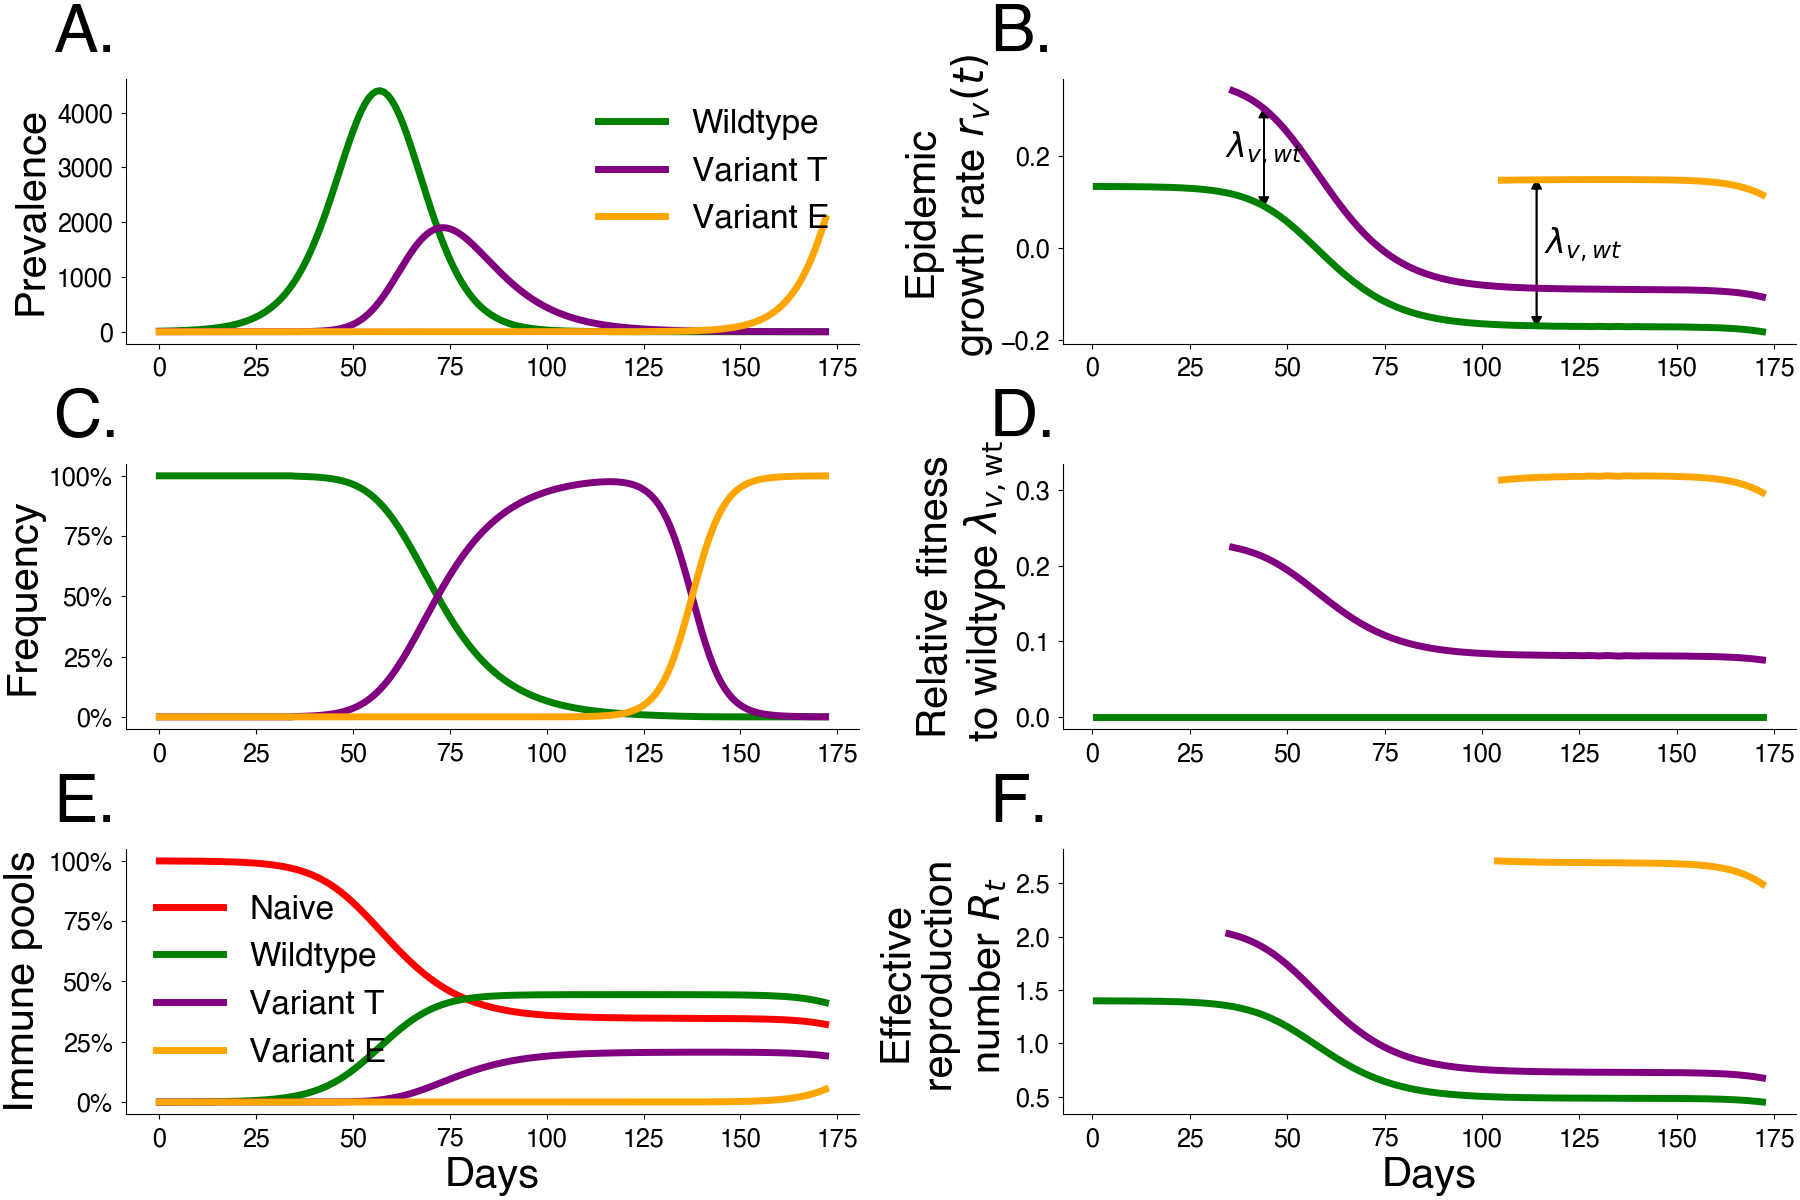
\includegraphics[width=1.0\linewidth]{./figures/vis_mechanisms.png}
    \caption[\textbf{Simulated variant dynamics in a mechanistic model.}]{
      \textbf{Simulated variant dynamics in a mechanistic model.}
      Mechanistic transmission models constrain variant frequency dynamics by specifying a functional form for relative fitnesses.
      Simulations of a three-variant model including wildtype $W$, an intrinsic transmission variant $T$, and an immune escape variant $E$ show the relationship between population-level transmission and selection.
      We begin the simulation with initial wildtype prevalence $I_\wt(0) = 1$, effective reproduction number $R_{0,\wt} = 1.4$, and duration of infection $1/\gamma = 3.0$ days.
      We introduce transmissibility variant $T$ at $t=20$ with frequency $f_T(20) = 10^{-5}$ and a 50\% increase in transmissibility $\varTransmission_T = 0.5$.
      We introduce escape variant $E$ at $t=70$ with frequency $f_E(70) = 10^{-6}$ that infects 5\% of hosts possessing wildtype immunity $\varEscape_E = 0.05$.
      A. Prevalence $I$ by variant.
      B. Exponential growth rate $r$ by variant.
      C. Variant frequency $f$.
      D. Fitness relative to wildtype $\lambda$.
      E. Underlying immune pools.
      F. Effective reproduction number $R_t$ by variant.
    }
    \label{fig:vis_mechanisms}
\end{figure}

% \subsection*{Estimating relative fitness using Gaussian Processes}

Our approach shows that relative fitness is often dependent on the past exposure of a population (as discussed in Supplementary Text \ref{ssec:frequency_dynamics} and extended to full immune history models in Supplementary Text \ref{ssec:full_immune_history}).
This suggests that serology, vaccination history, and immunological data generally can be informative of relative fitness.
Additionally, when working with variant classifications, non-neutral evolution within a variant will cause the relative fitness of that variant to change in time.
However, even in the absence of external data that can inform relative fitness, there is still hope.

We develop a method for using approximate Gaussian processes to model variant relative fitness.
Gaussian processes are probability distributions over functions, where the structure and smoothness of these functions are defined by a kernel that encodes correlations in time.
These models are flexible and allow us to encode smoothness constraints, periodicity, and other structures \cite{Gortler2019a}.
Gaussian processes allow us a non-parametric estimate of the relative fitness for variants through time (see Materials and Methods).

Traditional Gaussian process, while flexible, face challenges for large time series and large data sets.
Our approach overcomes this using a Hilbert Space Gaussian Process (HGSP) approximation, making the framework scalable for many variants and long time periods \cite{riutortmayol2022practical}.
This enables real-time variant fitness estimation and can be applied to any frequency data regardless of the underlying mechanism.
This model is used in Fig.~\ref{fig:gp_example} to estimate the relative fitnesses of different variants through time based on simulated variant sequence counts from frequencies shown in Fig.~\ref{fig:vis_mechanisms}.

Later, we apply this model to empirical SARS-CoV-2 sequence data from 50 US states and England from 2021 to 2022 to estimate relative fitness for variants circulating in that period, but first we continue analytic investigation into fitness dynamics.

\subsection*{Determining the transmisibility-escape tradeoff}

To understand the fitness trade-off between transmissibility and immune escape, we consider dynamics with a wildtype virus $\wt$ with $\varTransmission_\wt = 0$ and $\varEscape_\wt = 0$, an increased transmissibility variant $\varT$ with $\varTransmission_\varT > 0$ and $\varEscape_\varT = 0$ and an immune escape variant $\varE$ with $\varTransmission_\varE = 0$ and $\varEscape_\varE > 0$.

Following Equation \ref{eq:two_strain_relative_fitness}, we write relative fitnesses of the escape variant or transmissibility variant as
\begin{align*}
    \lambda_{\varE, \wt} &= \varEscape \beta \phi_{\wt}(t)\\
    \lambda_{\varT, \wt} &= \varTransmission \beta S(t).
\end{align*}

In the simplest case where individuals are either susceptible or have wildtype immunity ($S(t) + \phi_{\wt}(t) = 1$), we can compute the critical immune fraction $\phi^{*}$ at which $\lambda_{\varE, \wt}(\phi^{*}) = \lambda_{\varT, \wt}(\phi^{*})$ as
\begin{equation} \label{eq:critical_immunity}
    \phi^{*} = \frac{\varTransmission}{\varEscape + \varTransmission}.
\end{equation}

For past exposure level greater than $\phi^{*}$ escape variants have a higher relative fitness.
This trade off shows that increasing degree of escape entails that a lower proportion of past exposure is needed for escape variants to be preferred (Fig.~\ref{fig:transmission_tradeoff}).
Additionally, this shows that when intrinsic transmissibility increases are limited escape is more likely to be a dominant mechanism for variant turnover.

\begin{figure}[h]
    \centering
    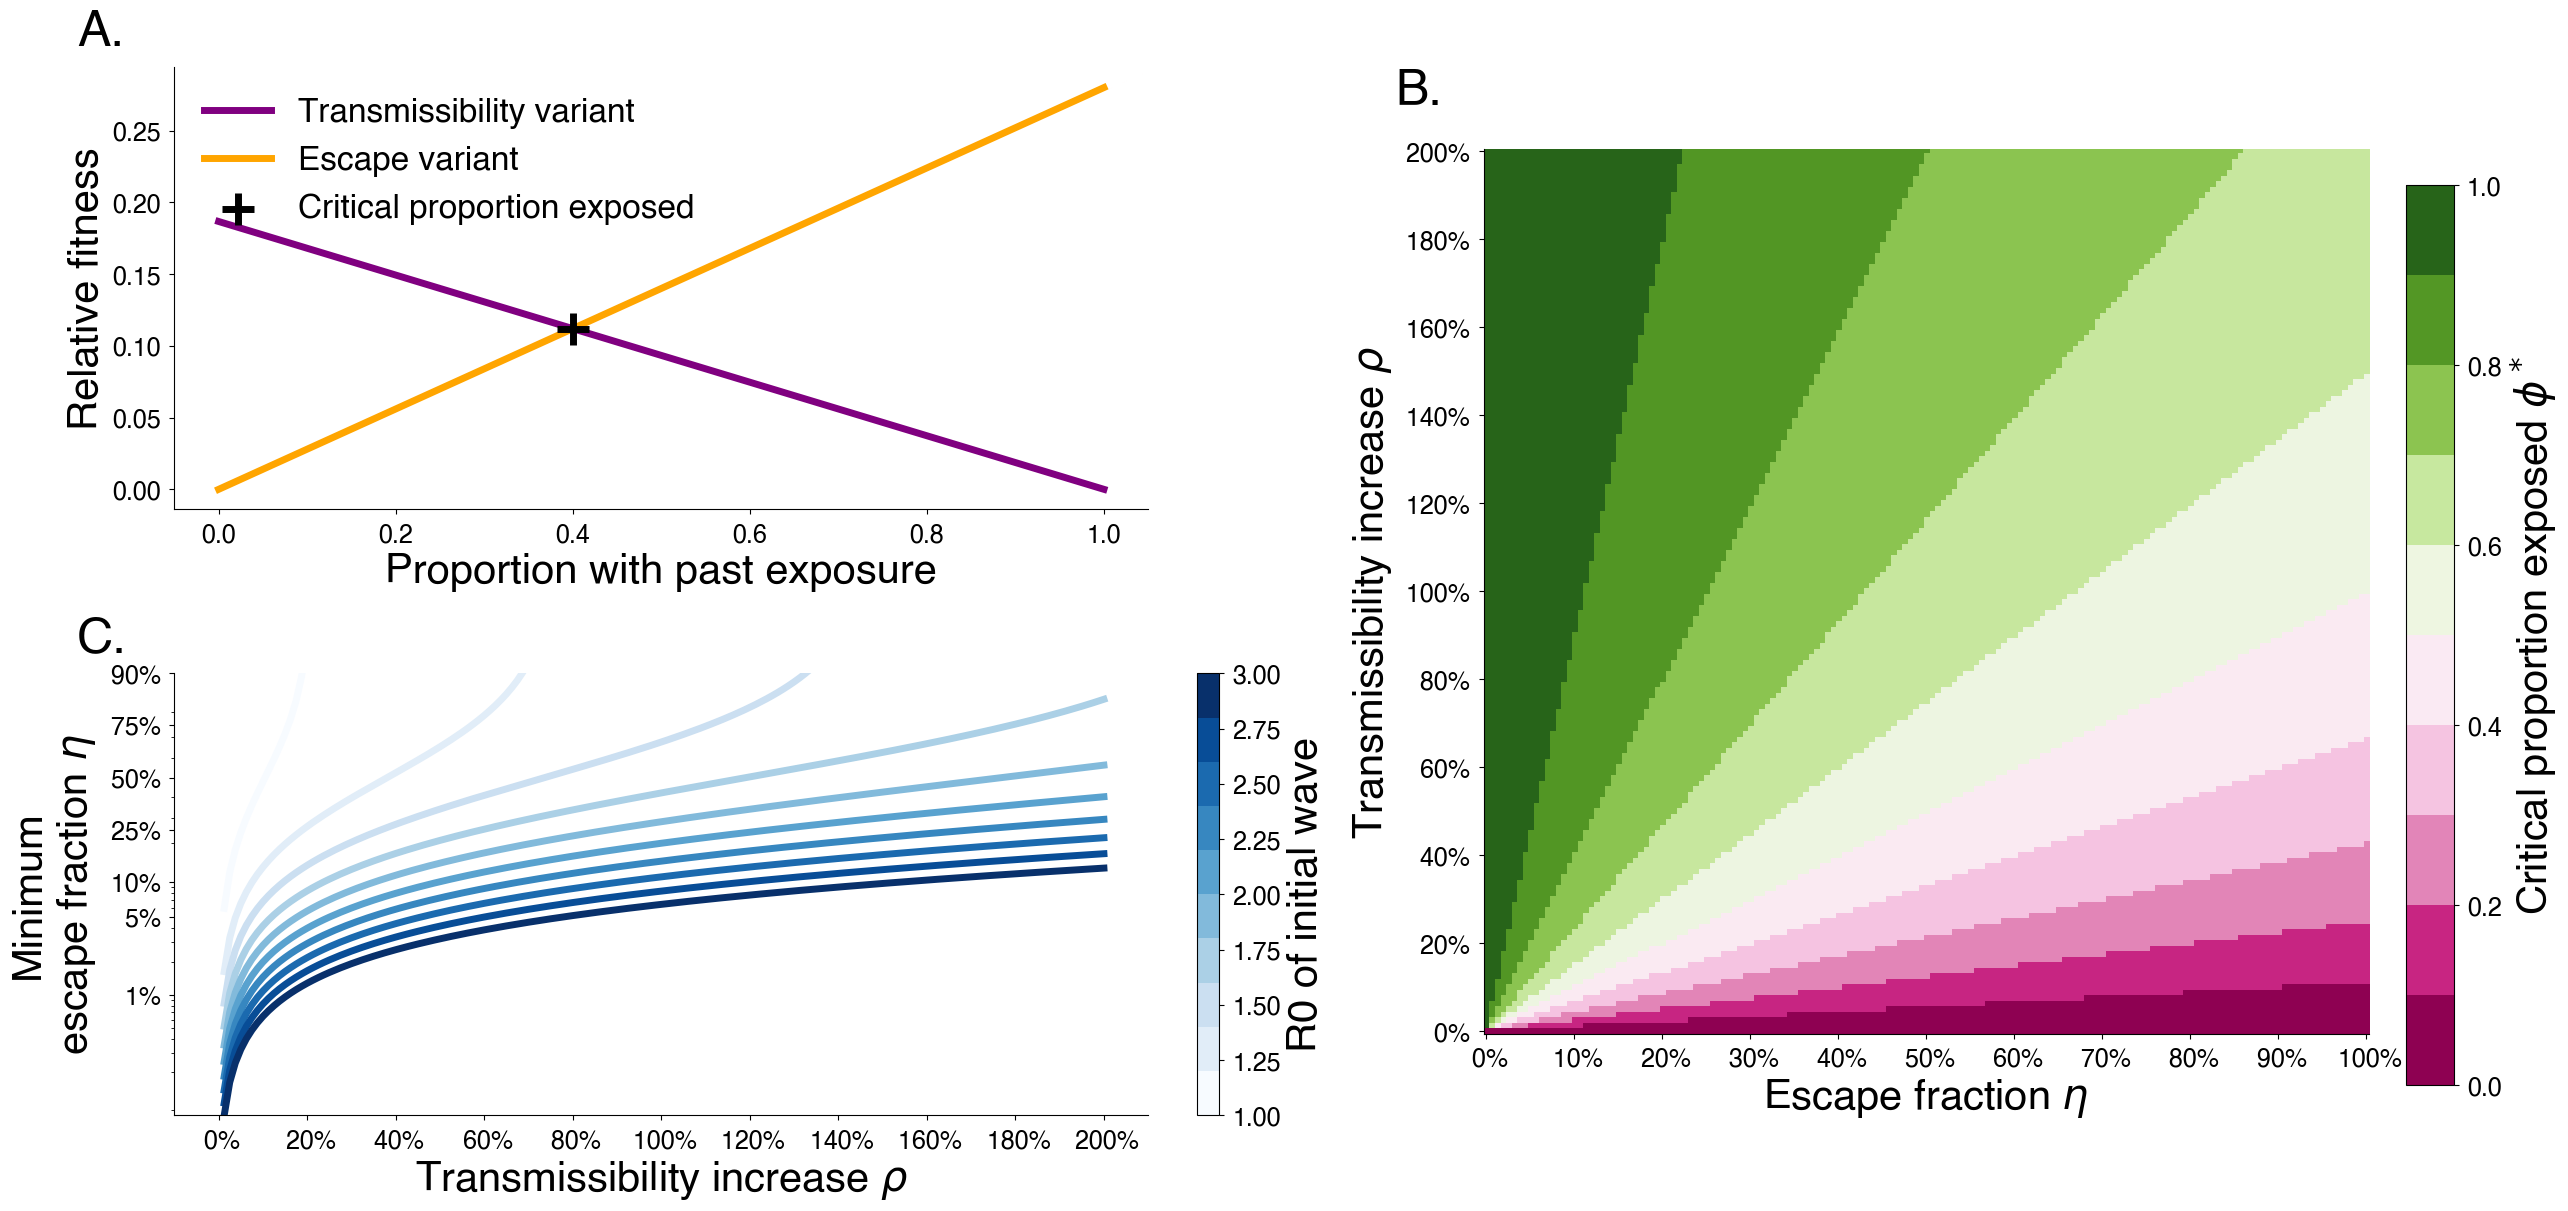
\includegraphics[width=1.0\linewidth]{./figures/transmission_tradeoff.png}
    \caption[\textbf{Trade-off between degree of immune escape and increased transmissibility.}]{
      \textbf{Trade-off between degree of immune escape and increased transmissibility.}
      A. Relative fitness for a transmissibility increasing variant $T$ with $\varTransmission_T=0.2$ and an immune escaping variant $E$ with $\varEscape_E=0.3$ for $R_{0, \wt}=2.8$ and $1 / \gamma = 3.0$ days.
      The intersection point shows that after 40\% of the population has wildtype immunity, the escape variant has higher fitness.
      B. The critical exposure proportion is shown for various escape fraction and transmissibility increase. Above the critical exposure proportion, we expect dominance of escape variants.
      C. The minimum escape fraction needed for second waves to be comprised of escape variant assuming competition with transmissibility increase variants and first wave with a given $R_{0}$.
    }
    \label{fig:transmission_tradeoff}
\end{figure}

\subsection*{Initial growth rates insufficient for predicting short-term frequency growth}

One question of interest is whether knowledge of mechanism meaningfully informs our ability to forecast short-term frequency growth.
The first step to addressing this is to understand how the relative fitness may change in time to understand the predictability of relative fitness in the short-term.

We find that the mechanistic forms analyzed in this paper (Supplementary Text \ref{ssec:frequency_dynamics}) can be represented as weighted combinations of $B$ time-varying functions $\Upsilon_{b}(t)$ with weights $\beta_{b}$.
We can think of each of these functions $\Upsilon_b$ as an immune background and the coefficient $\beta_{b}$ as a transmission differential, so that
\begin{align*}
\lambda_{v,u}(t) = \sum_{1 \leq b \leq B} \beta_{b} \Upsilon_{b}(t).
\end{align*}

Even in the case of complete knowledge of the relative fitness and the underlying fitness contributions in the present and past, we have that change in the relative fitness is determined by
\begin{align*}
    \frac{d\lambda_{v,u}}{dt} = \sum_{1 \leq b \leq B} \beta_{b} \frac{d\Upsilon_{b}}{dt}(t).
\end{align*}
By considering a Taylor expansion of the relative fitness about the point of estimation $t_{0}$, we can approximate the relative fitness in the future as:
\begin{align*}
    \lambda_{v,u}(t) \approx \lambda_{v,u}(t_{0}) + (t - t_0)\sum_{1\leq b \leq B} \beta_b \frac{d\Upsilon_b}{dt}(t_0).
\end{align*}
This suggests small differences in the form of $\lambda_{v,u}(t)$ can lead to meaningful differences in the future relative fitnesses through changes in the underlying immune backgrounds.

We investigate whether relative fitnesses vary predictably in the short-term regardless of mechanism.
To do so, we apply the two-variant model developed in previous sections for different mechanisms of immune escape and increased transmissibility.
We fix the relative fitness of the novel variant at a prediction time $t_{0}$ using Equation \ref{eq:critical_immunity} and assess the change in the relative fitness in the short-term.
We find that although relative fitness trajectories share the same decreasing shape, they may decline at different rates depending on the mechanism (Fig.~\ref{fig:short_term_divergence}).
This can lead to substantial changes in the predicted incidence depending on the assumed mechanism and affects to overall rate of turnover.

\subsection*{Correlations insufficient for mechanism identification}

Although correlations between vaccination uptake and variant growth advantage are often observed, these are alone may not be sufficient to identify the mechanism behind a variant's success.
A variant’s fitness advantage may arise from increased transmissibility, immune escape, or a combination of both.
Even in the absence of immune escape, the relative fitness of a variant depends on the proportion of the population that is susceptible to infection and therefore changes with both past exposure and vaccine uptake (Supplementary Text \ref{ssec:frequency_dynamics}).
To illustrate this, we simulate the spread of a variant with increased transmissibility in populations with varying initial vaccination levels.

In populations with lower vaccination levels, the variant’s prevalence peaks more sharply and its relative fitness declines quickly as immunity accumulates within the population (Fig.~\ref{fig:mechanism_identification}A-C).
In contrast, higher vaccination levels constrain relative fitness, leading to a delayed peak in prevalence and more stable relative fitness as the existing immunity limits the variant’s spread (Fig.~\ref{fig:mechanism_identification}A-C).
Even without immune escape, estimated growth advantages for this variant decrease with increasing vaccination uptake near the beginning of an epidemic (Fig.~\ref{fig:mechanism_identification}D).
Later in the epidemic, this relationship reverses with estimated growth advantages over the full period increasing with initial vaccination levels, which may be mistaken as signal for immune escape (Fig.~\ref{fig:mechanism_identification}E).
% At very high vaccination levels, we see the estimated growth advantage falls off sharply when both variants are declining in prevalence.
% This occurs at a critical vaccination threshold of $1 / R_v$ where $R_v$ is the effective reproduction number of the variant (Fig.~\ref{fig:mechanism_identification}E).

\begin{figure}[h]
    \centering
    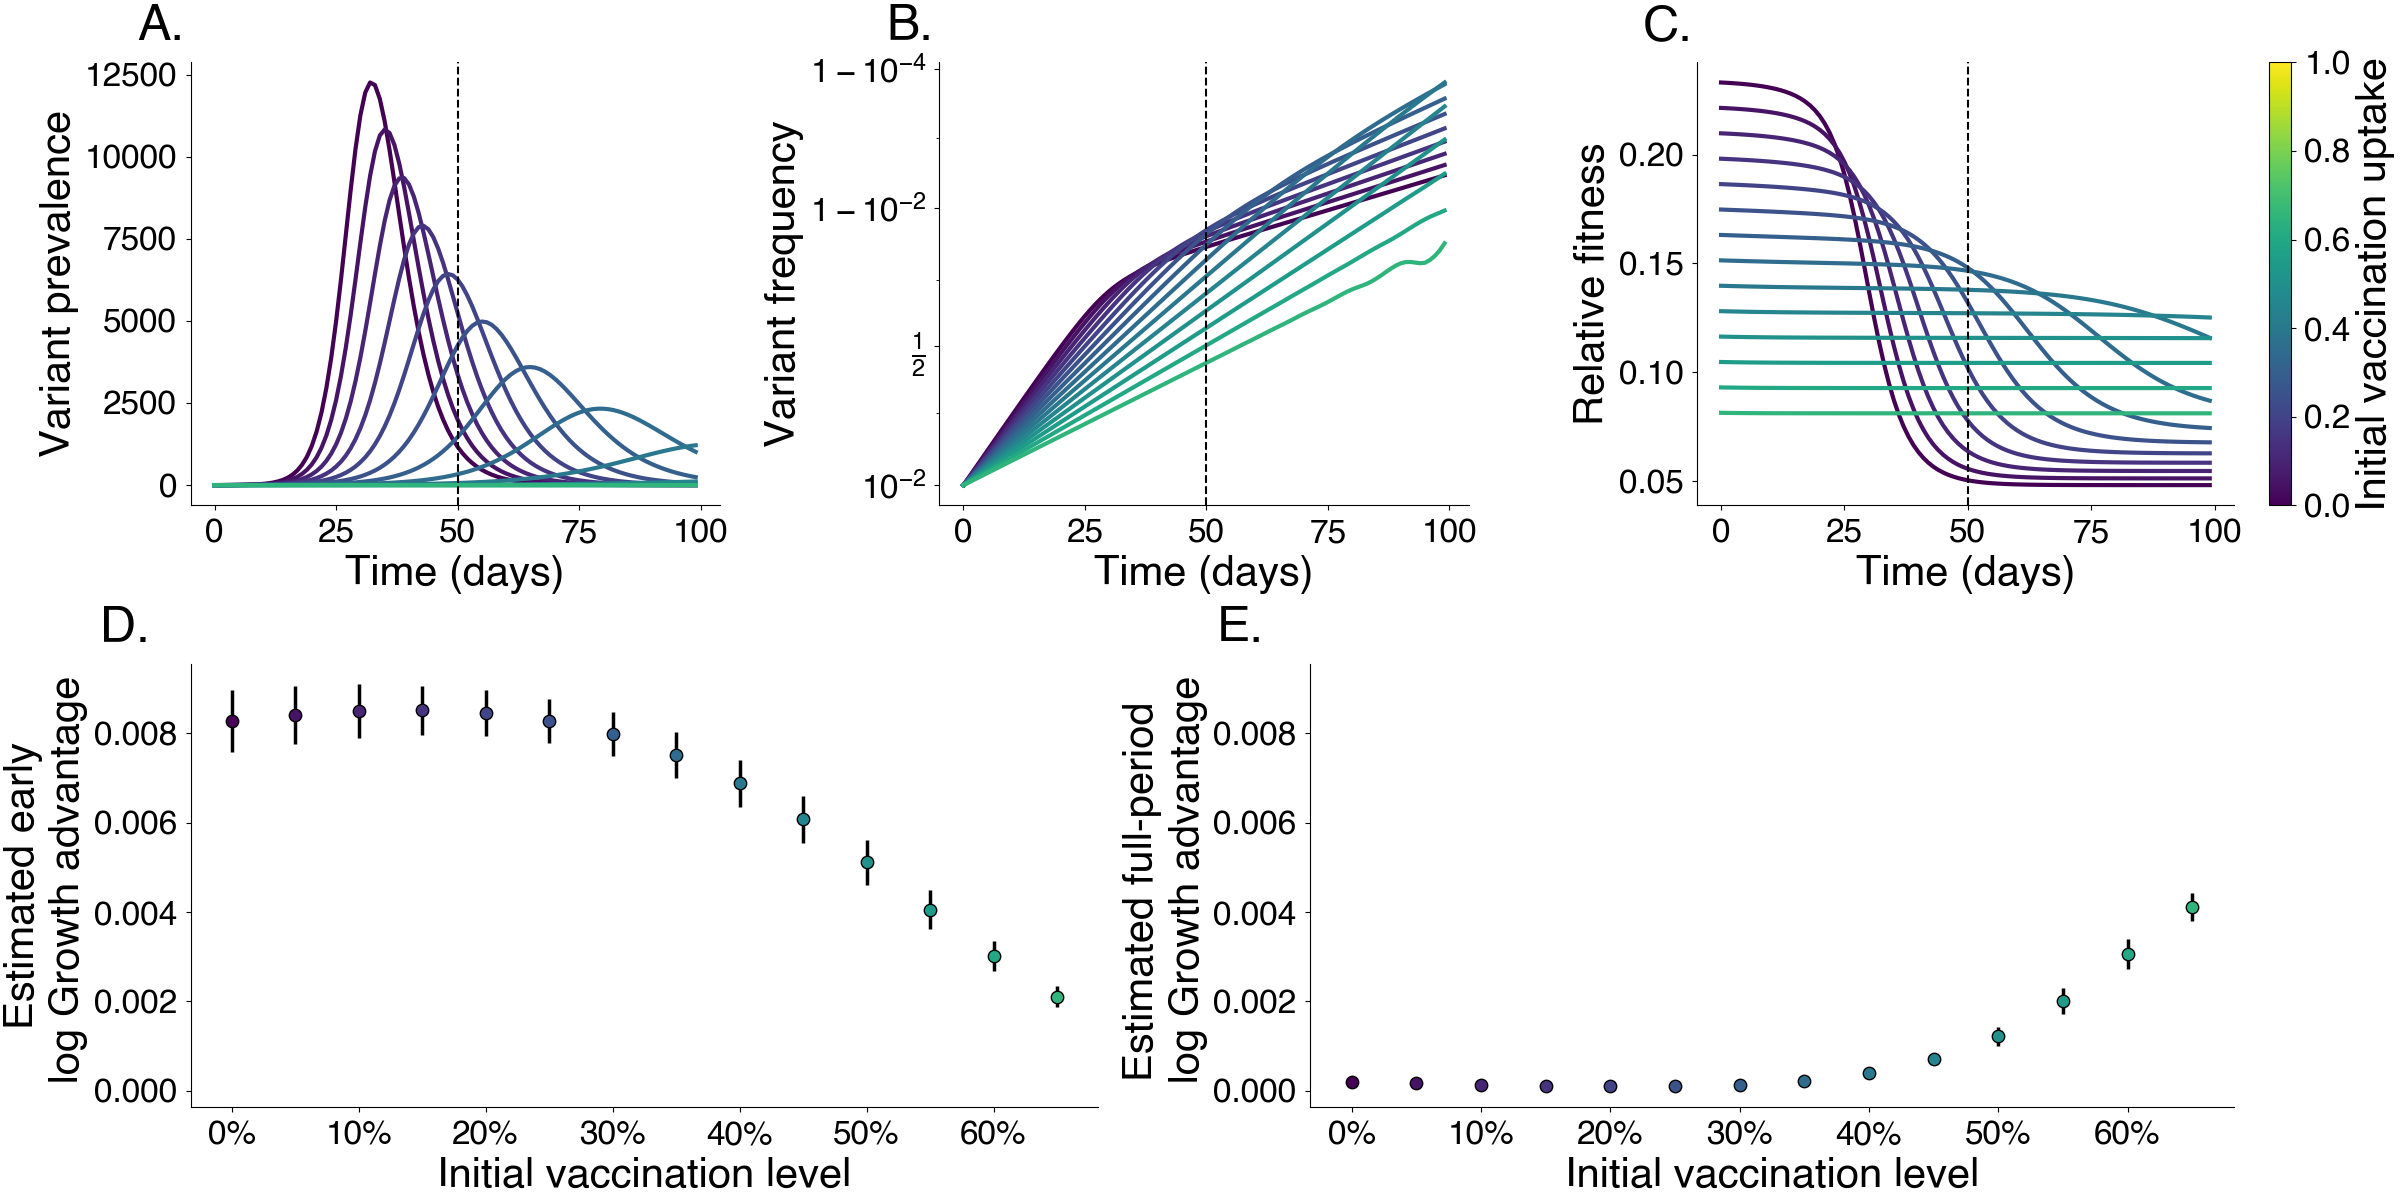
\includegraphics[width=1.0\linewidth]{./figures/mechanism_identification.png}
    \caption[\textbf{Relative fitness is correlated with vaccination levels in the absence of immune escape.}]{
      \textbf{Relative fitness is correlated with vaccination levels in the absence of immune escape.}
      We simulate the growth of a pure transmissibility increased variant at varying levels of vaccination.
      Darker colors represent lower vaccine uptake.
      We identify an early growth period where relative fitness is at its highest; the cutoff for this period is denoted with a vertical dashed line.
      A. Prevalence of variant, each line is its own simulation.
      B. Frequency of variant.
      C. Relative fitness for variant over time.
      D. Estimated log growth advantage using linear regression of log relative frequency of variant over wildtype using only data before the early cutoff.
      E. Same as D. but using data from the entire period shown.
    }
    \label{fig:mechanism_identification}
\end{figure}

% This analysis shows a limitation in the ability of correlation-based analyses on growth advantage to identify the underlying mechanisms of variant fitness.
% By explicitly accounting for the dynamics of immunity and transmissibility within populations, incorporating epidemiological structure in these models might provide a good foundation for understanding variant success under assumed or scientific-motivated mechanisms and enable comparison between competing mechanisms.

This analysis shows that correlation-based methods alone may struggle to identify the true mechanisms driving a variant’s success especially under the assumption of a fixed growth advantage.
By explicitly considering how immunity and transmissibility interact within populations, models that incorporate these dynamics may provide a stronger foundation for understanding why certain variants spread.
% This approach also enables clearer comparison between different potential mechanisms behind variant fitness.

% Variant growth advantages can be correlated with vaccination proportions even in the absence of immune escape.
% Simulated multiple epidemics of a pure increased transmissibility variant at varying levels of initial vaccination and was able to see that estimated growth advantages, computed using a logit linear model, were correlated with initial vaccination fraction.
% We find that you can estimate association of increased relative fitness due to vaccination in the absence of immune escape (Fig.~\ref{fig:mechanism_identification}).
% This appears to hold up until both variants' initial effective reproduction number is below 1 i.e. $V_{0} > 1 / R_{v}$.

\subsection*{Quantifying selective pressure}

Although it is useful to quantify the relative fitnesses of individual variants, we are often interested in quantifying the overall effects of selection in the population.
With this in mind, we can derive a metric of overall selective pressure $\psi(t)$ which describes the distribution of relative fitness in the population
\begin{equation}
\psi(t) =  \Expect_{f(t)}\left[ \frac{d \lambda_v}{d t}\right] +  \Var_{f(t)}[\lambda_{v}].
\end{equation}
This selective pressure metric serves as an indicator for high fitness variants arising in the population as change.
High fitness variants rising from initially low frequency leads to large increases in the variance of the fitness distribution and therefore increases in the selective pressure.

The selective pressure metric enables us to decompose changes in the average growth rate in the population $d\bar{r}/dt$ to an evolutionary component $\psi$ and a residual baseline growth rate $r_\wt$ following
\begin{equation}
    \frac{d\bar{r}}{dt} = \frac{dr_{\wt}}{dt} + \psi(t).
\end{equation}
This shows that increased selective pressure through emerging high fitness variants can drive waves of infection.
Further, this suggests that differences between growth rates based on selective pressure alone and observed rates are attributable to changes in baseline transmission over time.
This mirrors ideas of Fisher's theorem of natural selection and its later interpretations with the variance of fitness contributing directly to the change in transmission rates (or fitness) \cite{Ewens1989, Ewens2024}.
This definition of selective pressure captures how relative fitness contributes to epidemic growth.
This is similar to ideas quantifying rates of adaptation via fitness flux \cite{Mustonen2010}.

In this case, the overall growth rate $\bar{r}$ and relative incidence $I(t) / I(0)$ can be written directly using the cumulative selective pressure $\Psi(t) = \int_0^t \psi(s)ds$ as follows:
\begin{align}
    \bar{r}(t) &= \bar{r}(0) + [r_{\wt}(t) - r_{\wt}(0)] + \Psi(t)\\
    \frac{I(t)}{I(0)} &= \exp \left( \int_0^t [r_{\wt}(s) + \Psi(s)]ds \right).
\end{align}
In addition to estimating the relative fitness, metrics derived from these models can be informative of much more.

Our ``selective pressure'' metric which allows us to model the contribution of evolution to changes in the epidemic growth rate of a population and is independent of pivot choice for relative fitness estimation.
This metric acts as an early warning system for variant-driven outbreaks, especially in scenarios where case data are sparse or delayed.
This metric can be computed using any method that estimates variant frequency and relative fitnesses and serves as a simple tool for understanding the contribution of selection to the overall population dynamics.
% This approach is compatible with any method which estimates frequency and relative fitness, enabling broad applicability to many pathogens.

The full derivation of this metric and its contribution to the overall growth rate can be found in Supplementary Text \ref{ssec:deriving_selective_pressure}.

\subsection*{Predicting epidemic growth rates using selective pressure}

Motivated by the relationship between epidemic growth rate and selective pressure demonstrated above, we develop a predictive model of epidemic growth rate using estimates of selective pressure.
% By integrating fitness estimates and variant frequency dynamics, selective pressure can be used to predict epidemic growth rates, empowering public health agencies to anticipate and respond to new variant-driven outbreaks.
Using empirical SARS-CoV-2 case and sequence data from 50 US states between January 2021 and November 2022, we estimate epidemic growth rates through time in each state using case counts, and estimate selective pressure through time using our approximate Gaussian process model on sequence counts  (Fig.~\ref{fig:selective_pressure_prediction} A--C.)
Here we group variants at the granularity of Nextstrain clades \cite{aksamentov2021nextclade} resulting in 28 distinct variants over this time period.
As expected we see that relative fitness increases through time and that selective pressure corresponds to speed of clade turnover where the sweep of Omicron BA.1 (clade 21K) yields the strongest signal of selective pressure (Figs.~\ref{fig:selective_pressure_group_1}--\ref{fig:selective_pressure_group_5}).
We use these estimates to fit a gradient-boosted regressor to predict epidemic growth rates using selective pressure from the most recent 28 days, reserving data between July 2022 and November 2022 for testing (Fig.~\ref{fig:selective_pressure_prediction} D--I, Fig.~\ref{fig:empirical_growth_rate_predictions_all}).
This regressor is chosen via time series cross-validation among model architectures and grid-search parameter tuning (Fig.~\ref{fig:growth_rate_predictions_model_comparison}).

\begin{figure}[h]
    \centering
    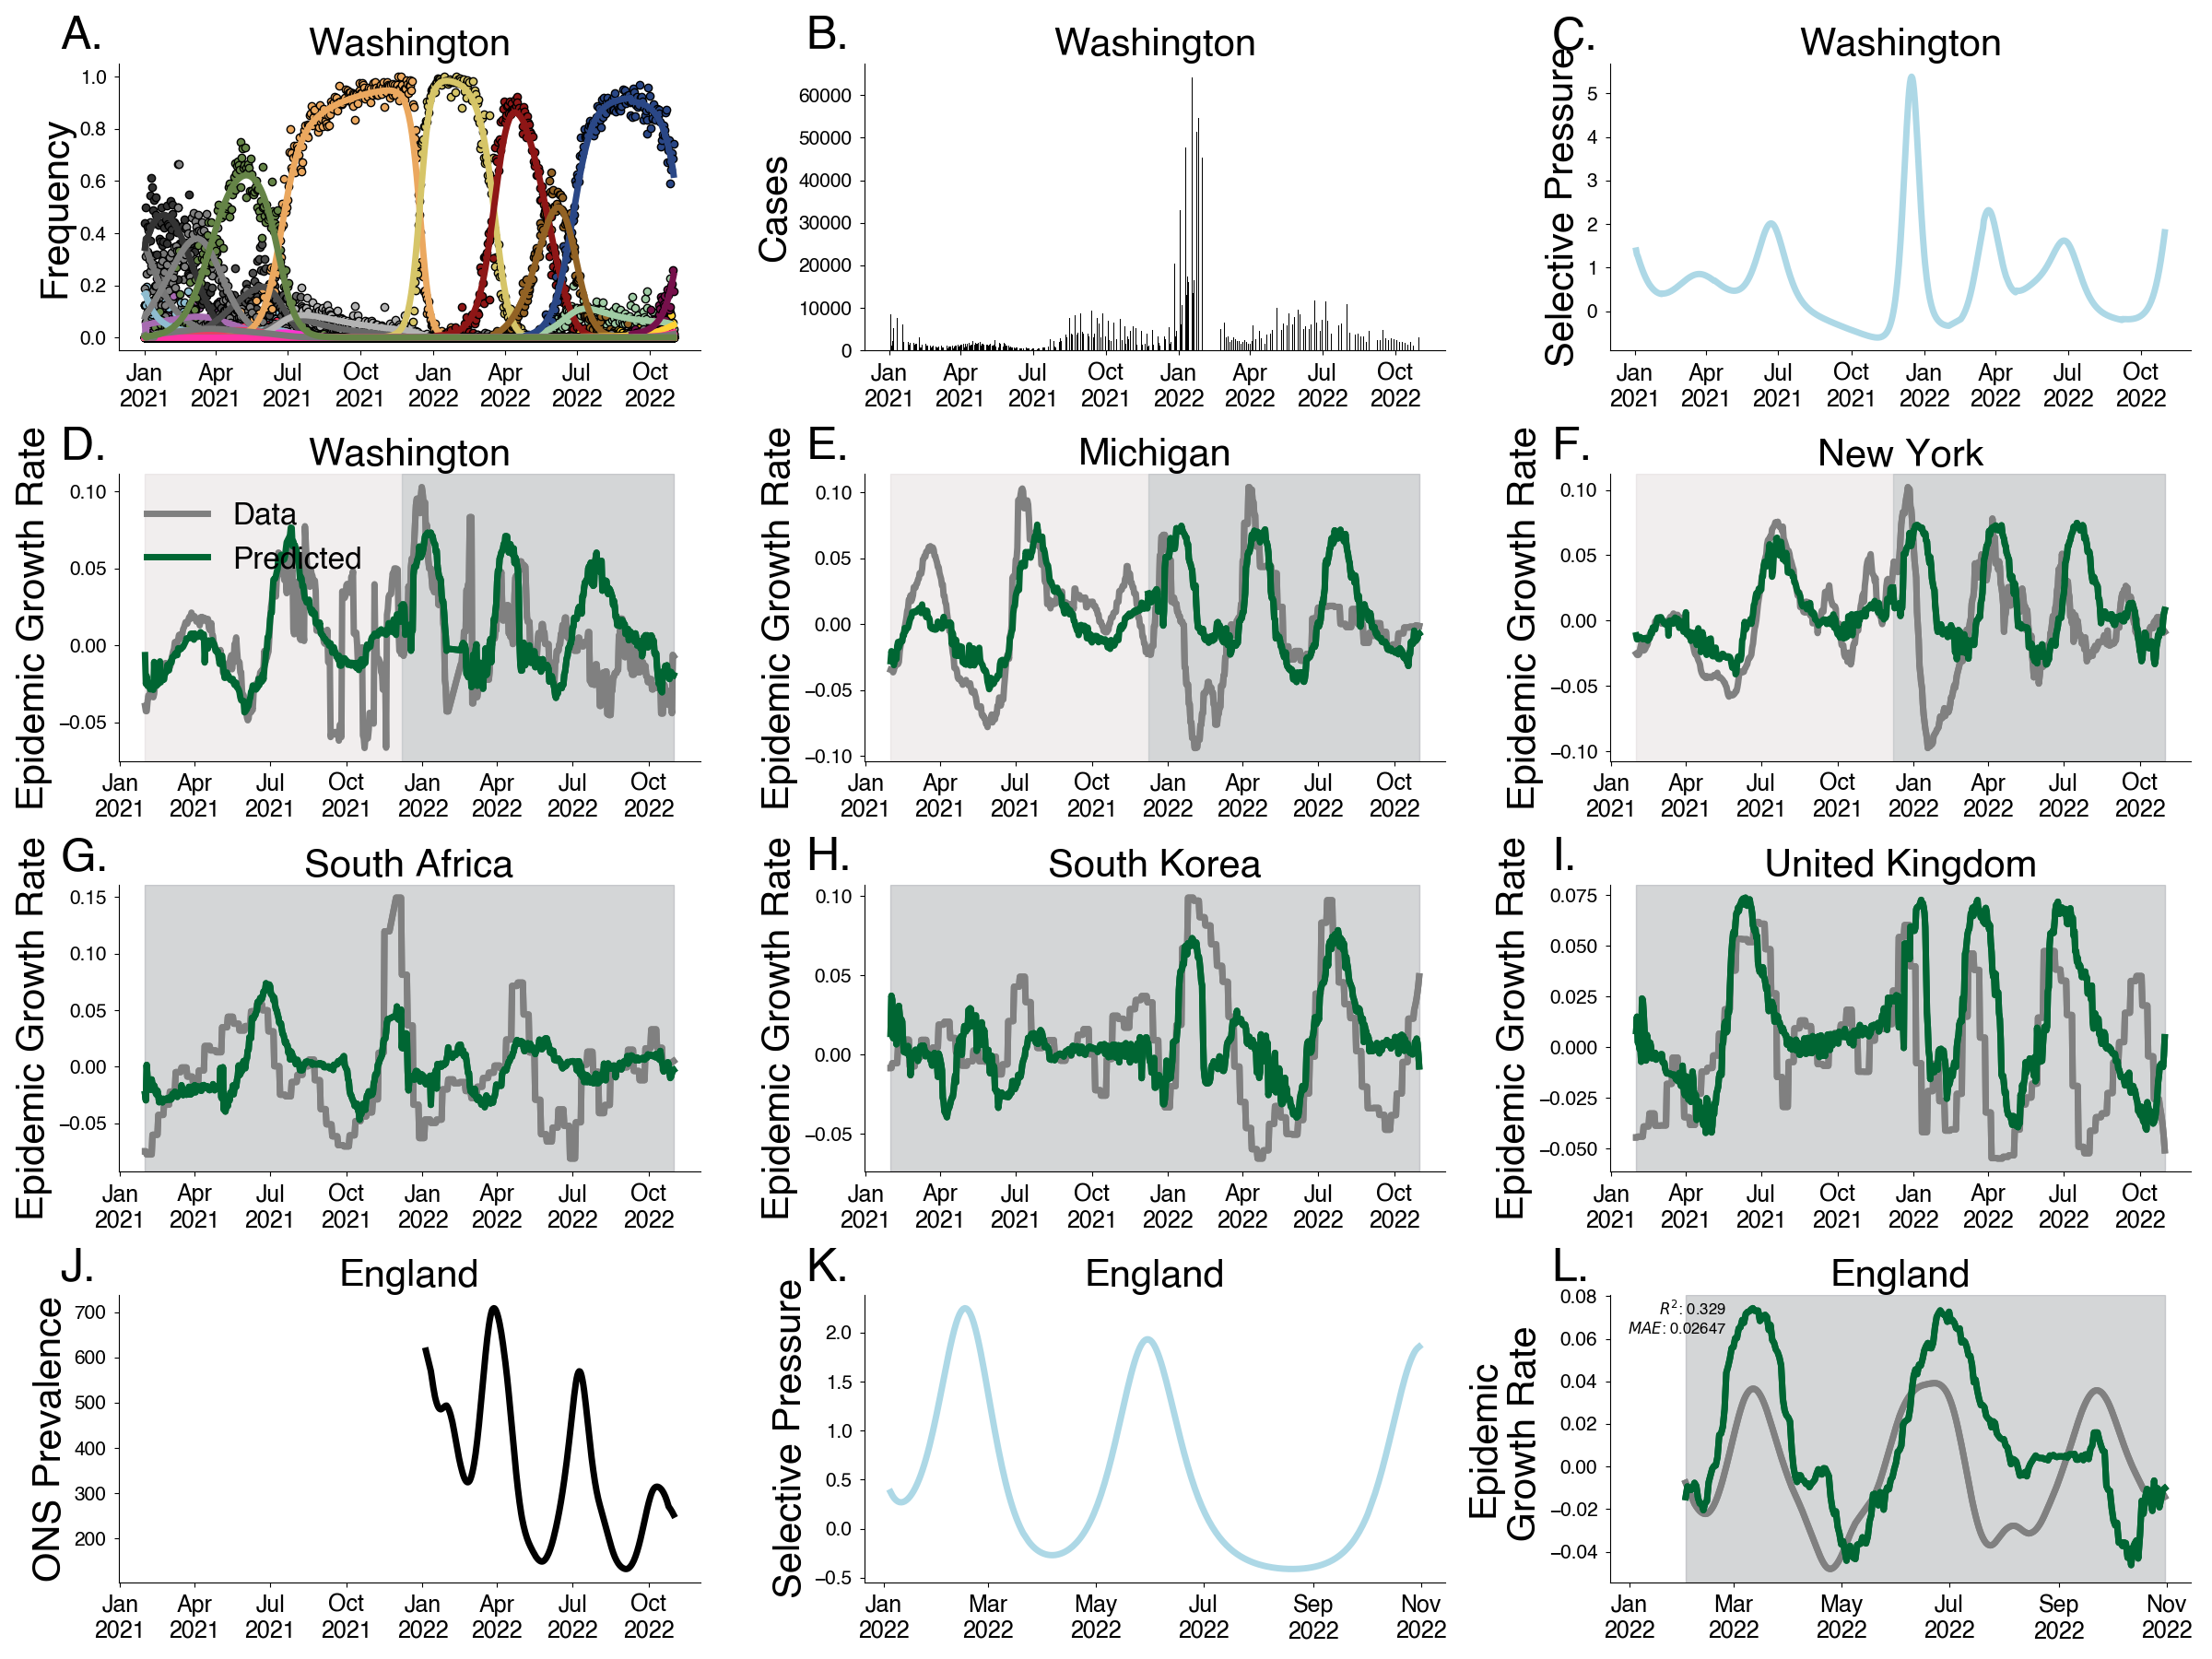
\includegraphics[width=1.0\linewidth]{./figures/selective_pressure_prediction.png}
    \caption[\textbf{Predicting epidemic growth rate using estimated selective pressure.}]{
      \textbf{Predicting epidemic growth rate using estimated selective pressure.}
      A. Variant frequency estimated using the Gaussian process relative fitness model between January 2021 and November 2022 for sequence count data from Washington state.
      B. Case counts from Washington state.
      C. Selective pressure computed using estimated variant frequencies and relative fitnesses from Washington state.
      D-F. Predictions for empirical growth rate from selective pressure for selected US states.
      The light gray period is the training period and the darker gray is the testing period.
      G-I. Predictions for empirical growth rate from selective pressure for countries South Africa, South Korea and the UK.
      J. Prevalence estimates for England from ONS Infection Survey.
      K. Estimated selective pressure in England.
      L. Empirical growth rates (gray) computed from prevalence estimates and predictions from our model (green) computed from selective pressure.
    }
    \label{fig:selective_pressure_prediction}
\end{figure}

We observe a strong correspondence between observed epidemic growth rate and model predictions with Pearson $R^2$ in the training period of 0.576 and a weaker Pearson $R^2$ in the testing period of 0.077.
As case reporting declined over this period, we expect weaker correspondence between our predictions and epidemic growth rates computed from case data.
To address this, we sought to evaluate the out-of-sample fit on case data from other countries e.g. South Africa, South Korea, and the United Kingdom, achieving an $R^2$ of $0.196$.

To address the potential for this method under steady reporting rates, we validate this method by predicting the epidemic growth rates in England derived from the Office for National Statistics (ONS) Coronavirus Infection Survey between February 2022 and November 2022.
The ONS Infection Survey represented a randomly sampled panel survey of households where nasal swabs were collected regardless of symptom status allowing for prevalence estimates despite faltering case reporting \cite{pouwels2021community}.
Our model is able to replicate patterns seen in epidemic growth rates in England derived from ONS data (Fig.~\ref{fig:selective_pressure_prediction} J--L), achieving a coefficient of variation of $R^2 = 0.329$ and mean absolute error of 0.026.
Performance is significantly better for the first two subsequent waves, falling off in accuracy for the fall 2022 BQ.1 (clade 22E) wave.

Although these predictions can be biased by non-evolutionary effects on the epidemic growth, this approach provides a simple measure of epidemic growth in the absence of high quality case counts using sequence data alone.

\subsection*{Latent factor model of relative fitness}

The representation of relative fitness using discrete immune backgrounds suggests that there may be low-dimensional structure to variant relative fitness.
To generate pseudo-estimates of this latent factors, we develop and implement our method for latent factors models of relative fitness.
This model assumes that variants intrinsically escape the immune responses with particular groups and that differences in a variant's relative fitness between geographies is attributable to differences in immunity between populations.
This enables us to estimate a pseudo-escape rates for variants as well as pseudo-immunity groups within geographies over time.

We generate Pango lineage-level sequence counts for 18 countries and 53 variants between March 2023 and March 2024.
These 18 countries were chosen based on availability of sequence data.
Small lineages which do not meet a count threshold are collapsed into their parent lineages.
This leaves us with a total of 53 variants, so that each variant met a threshold for number of sequences available.

Using these sequence counts, we apply our latent factor model to estimate the relative fitness of each variant over time in each country, pseudo-escape rates for each variant, and pseudo-immunity for each country simultaneously for $D=10$ pseudo-immune groups.
This model is significantly constrained relative to estimating the time-varying fitness independently in each location, resulting in a model with 2,752 parameters compared to 7,488 parameters in the independent model.

The results of this model are visualized in Fig.~\ref{fig:latent_immune} for several selected variants and countries of interest.
Our results show that closely related Pango lineages are often assigned similar pseudo-escape values suggesting that this is capturing some evolutionary structure to immune escape.
Further, our model shows that these groups of lineages tend to target particular immune groups such as clade 24A (JN.1, JN.1.1, JN.1.4) has high pseudo-escape in dimensions 3 and 4.
If immune escape is the dominant mechanism for relative fitness difference, we expect that differences in immune response between variants from serological data would mirror differences in our pseudo-escape space.
Using human serological data from Jian et al \cite{Jian2023}, we compute titer distances as average log2 differences in titer values between pairs of variants.
We compare these distances to distances in our pseudo-escape space (Fig.~\ref{fig:latent_immune}G), finding the distances between distinct pairs in the pseudo-escape space are correlated with these titer differences between variants ($R^2$ = 0.402).
We bootstrap this analysis among 1,000 replicates to assess significance of this relationship (Fig.~\ref{fig:latent_immune_bootstrap}, $p < 0.001$).
Additionally, we subset by exposure history and find that cohorts with only very recent infection correlate more poorly than WT vaccine cohort or cohorts with more complex exposure histories (Fig.~\ref{fig:titer_distance_correlations_by_group}).

\begin{figure}[h]
    \centering
    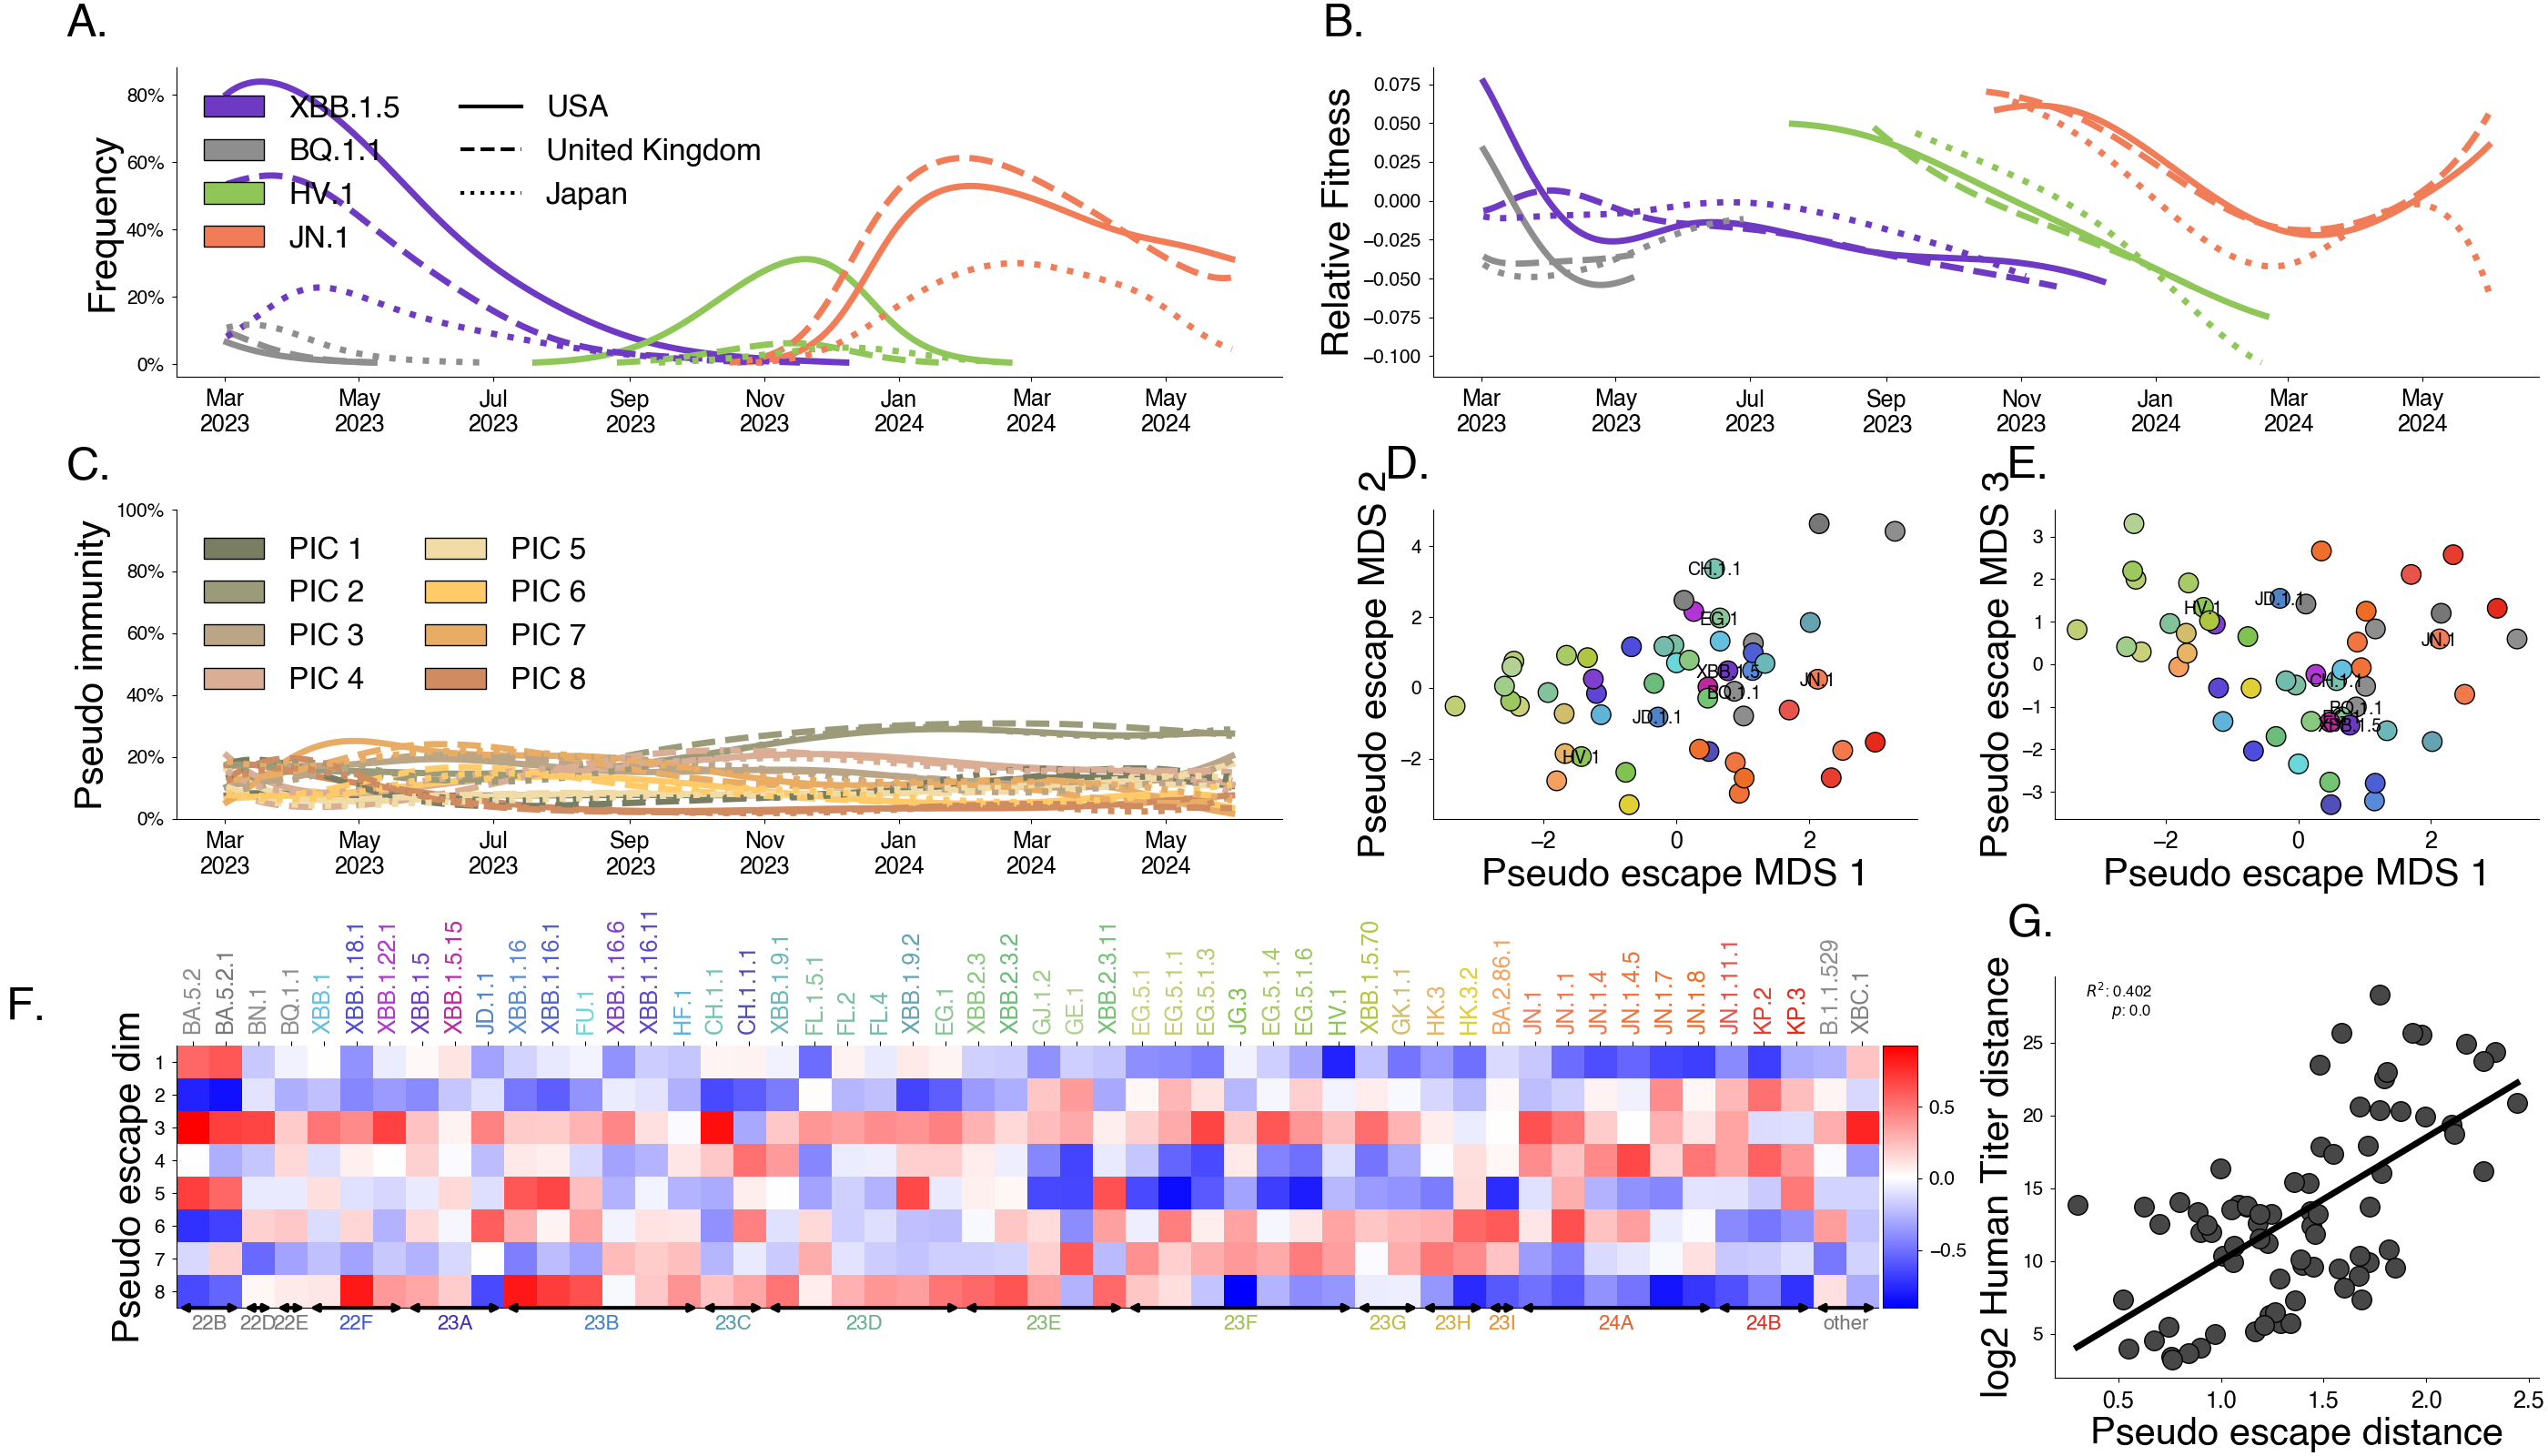
\includegraphics[width=1.0\linewidth]{./figures/latent_immune.png}
    \caption[\textbf{Latent factor models of immunity describe variant dynamics.}]{
      \textbf{Latent factor models of immunity describe variant dynamics.}
      We fit the latent immunity factor model to recent SARS-CoV-2 sequence data globally.
      A. Variant frequency. Lines are colored to show 4 variants of interest (of 53 total variants) with the style of the line denoting 3 countries of interest (of 18 total countries).
      B. Estimated relative fitness for selected variants and countries.
      C. Estimated pseudo-immunity cohorts (PIC) over time for multiple countries ordered by decreasing share in the first geography
      D, E. Dimensionality-reduced pseudo-escape rates using multidimensional scaling (MDS).
      F. Estimated pseudo-escape rates for each variant relative to pivot variant.
      H. Comparing pairwise distance between variants in the pseudo-immune space to observed distances in human titer data.
    }
    \label{fig:latent_immune}
\end{figure}

We chose $D=8$ for our primary analysis by noting the point at which the loss function seems to stagnate with increasing $D$ i.e.\ the ``elbow'' method (Fig.~\ref{fig:latent_factor_dimension}A).
% \tbc{The text says that $D=10$ but figure \ref{fig:latent_immune} shows 8 groups. I believe that 8 is correct and I've corrected text accordingly. Please update if this was incorrect.}
% MF: Made slight changes to text here
Further, we observe that Bayesian Information Criterion (BIC) is minimized between 7 and 9 groups (Fig.~\ref{fig:latent_factor_dimension}D).
However, the exact choice of latent immune dimensionality is necessarily somewhat arbitrary and we observe significant correlations with empirical titer data for fewer dimensions as well, although $D=8$ also maximizes this correlation (Fig.~\ref{fig:latent_factor_dimension}B) and its significance is maintained for all dimensions $D > 8$ tested.
Analogous figures showing pseudo immunity and pseudo antigenic relationships across variants can be seen for $D=2$ in Fig.~\ref{fig:latent_factor_2}, $D=4$ in Fig.~\ref{fig:latent_factor_4}, $D=6$ in Fig.~\ref{fig:latent_factor_6} and $D=10$ in Fig.~\ref{fig:latent_factor_10}.

This approach can be applied to other antigenically variable, such as influenza, making it broadly applicable beyond SARS-CoV-2.
In fact, there is more utility for pathogens with larger geographic differences in immunity since this approach enables to estimate the proportion of these latent immune pools in the population and how they vary geographically and over time alongside variant difference.
By approximating antigenic differences using sequence data alone, this method offers for a deeper understanding of immune dynamics and how they shape variant success in the presence of immune escape.
This enables an embedding similar to those from antigenic cartography but without the need for serological data and based purely on observed variant fitness.

\subsection*{Conclusions, limitations, and future work}

Our study demonstrates the utility of multi-strain mechanistic models in interpreting variant frequency dynamics.
This enables a more detailed picture of variant success in environments with heterogeneous population immunity.
Our mechanistic grounding of variant fitness allows for investigations into trade-offs between intrinsic transmissibility increase and immune escape, prediction of epidemic dynamics from sequence data alone and inference of antigenic relatedness among variants from differences in success across geographies.

% One key insight from this was the trade-off between intrinsic transmissibility increase and immune escape.
% We showed that this trade-off is shifted by changes in population immunity, so that immune escape dominates as exposure increases.
% Though there are limits to our ability to attribute dynamics to particular mechanisms from frequency data alone, the structure of these models suggests that we may improve forecasting by incorporating information about empirically supported mechanisms such as immune escape via antigenic evolution.

Despite these advances, there are limitations to our approach.
Long-term forecasts remain difficult, particularly as new variants with unknown fitness profiles emerge.
This framework suggests that considering both the escape against individual immune backgrounds and the diversity in human immune escape is most useful for improving forecasts of relative fitness.
Additionally, our models, while powerful in estimating short-term variant dynamics, rely on assumptions about transmission mechanisms that may not always hold across different pathogens or contexts.
In fact, as we've shown, it's entirely possible for shifts in population immunity to change the dominant transmission mechanism.

Furthermore, the models considered here are deterministic in nature and do not explicitly model the emergence of variant viruses only the dynamics after their successful introduction.
In reality, there are biological constraints on the types of variants that are produced in nature and even if there is a `true' fitness boost, the chance for stochastic extinction of beneficial variants remains.
These constraints present trouble for long-term forecasting as it will require a model of mutation or emergence, tying the potential for a variant to emerge with its potential to transmit in the current environment.
Future work should focus on improving the integration of real-time genomic data with serological and epidemiological data, providing a more comprehensive understanding of variant dynamics over time.

% These ideas are already represented in existing literature through the form of long-term forecast models which incorporate phylogenetic and molecular data which is thought to be indicative of selection and immune escape. \cite{Huddleston2020, luksza2014predictive}

% Future work should seek to identify and integrative informative data sources for relative fitness estimation and forecasting for particular pathogens, providing a more comprehensive understanding of variant dynamics over time.

% Limitations of existing simple mechanism models
% The compartment models discussed here are described by simple mechanisms and more work is needed to adapt this framework to complicated epidemic models such as those with non-exponential generation times could be useful.
% That being said, models which account for the appearance of genetic variants through mutation exist, often assuming a latent antigenic space with which fitness is determined.
%
% However, it is important to note that these models may not be reliable for longer terms forecasts due to the emergence of new variants or improper specification of mechanism.

% Despite the limitations discussed above, the framework presented here illustrates the importance of transmission mechanism in the evolution of pathogens, highlighting the importance of both variant characteristics and population susceptibility in selection.
% We suggest that future models of pathogen transmission and evolution attempt to incorporate current knowledge of the transmission process into their forecasts.
% In particular, for viruses such as influenza and SARS-CoV-2 which undergo antigenic evolution, our work suggests that incorporating knowledge on both the diversity in human immune response and the escape potential of emerging variants could prove useful in improving long-term forecasts of the viral population.

In conclusion, our framework represents a significant advance in our understanding of viral evolution and transmission dynamics.
By linking variant fitness to specific transmission mechanisms, we provide a more nuanced and accurate prediction of how variants will spread and impact population-level epidemic growth.
The selective pressure metric and latent immunity model offer new tools for public health agencies to monitor viral evolution in real time, enabling proactive intervention and insight into the variant difference and wave potential.
While our work has been applied to SARS-CoV-2, the methods developed here are broadly applicable to other evolving pathogens, offering a versatile approach for improving epidemic forecasting, variant monitoring, and overall pandemic preparedness.

\subsection*{Acknowledgements}

We thank Ivana Bozic, Betz Halloran, Mark Kot and Erick Matsen, as well as members of the Bedford Lab for their feedback on this work.
We gratefully acknowledge all data contributors, ie the Authors and their Originating
laboratories responsible for obtaining the specimens, and their Submitting laboratories for generating the genetic sequence and metadata and sharing via the GISAID Initiative, on which this research is based.
We have included an acknowledgements table in the associated GitHub repository under \texttt{data/final\_acknowledgements\_gisaid.tsv.xz}.

\subsubsection*{Funding}

This work is supported by NIH NIGMS award R35 GM119774 to TB and a Howard Hughes Medical Institute COVID-19 Collaboration Initiative award to TB.
MDF is an ARCS Foundation scholar and was supported by the National Science Foundation Graduate Research Fellowship Program under grant No.\ DGE1762114.
TB is a Howard Hughes Medical Institute Investigator.

\subsubsection*{Author contributions}
MF conceived the study.
MF, TB gathered sequence and case count data.
MF designed and implemented the models.
MF performed the analysis.
MF, TB interpreted the results.
MF, TB wrote the paper.

\subsubsection*{Competing interests}

All authors declare no competing interests.

\subsubsection*{Data and materials availability}

Source code used to generate figures, model implementations, and sequence count data are available at \href{https://github.com/blab/relative-fitness-mechanisms}{github.com/blab/relative-fitness-mechanisms}.


% ========== Chapter 5
\graphicspath{{./chapters/ncov-escape/}}
\chapter{Forecasting SARS-CoV-2 lineage success from molecular data}

In this chapter, we develop and discuss methods for predicting relative fitness using molecular data.
We intend to expand this chapter into a larger paper.
This expanded paper will include analyses on how long the predictive power of molecular data lasts as well as more replicates of this idea for evolution post-BA.2 and post-JN.1.

\section{Abstract}

% Most methods are statistical.
% Though some theoretical work has been done to understand how mechanism informs relative fitness, there is still a need to build predictive model that can use data for this prediction.
%
% We develop methods for estimating and predicting relative fitness using evolutionary history and molecular data and leverage these methods to build models that enable out of sample prediction of relative fitness based on patterns of descent.
SARS-CoV-2 variants have driven global waves of infection, shifting from transmissibility-driven success in Alpha and Delta to immune escape in Omicron and its descendants.
Models estimating relative fitness from variant frequencies provide short-term insights but often fail in long-term forecasts due to dynamic fitness landscapes and neglect of evolutionary history.
Simulations reveal that this oversight inflates correlations between molecular phenotypes and fitness, misattributing patterns to ancestry rather than mechanism.
To address this, we introduce a Bayesian framework that integrates molecular phenotypes, such as immune escape and receptor binding, with phylogenetic structure.
By leveraging innovation-based regression priors, our method accounts for shared ancestry and fitness changes along lineages, enabling robust out-of-sample predictions.
This framework advances forecasting of SARS-CoV-2 variant success and offers a generalizable tool for understanding and responding to the evolution of rapidly mutating pathogens.

\section{Introduction}

The COVID-19 pandemic has been characterized by the emergence of SARS-CoV-2 variants that have driven successive waves of infection globally. %TODO: Bunch of citations
Early variants like Alpha, Beta, Gamma, and Delta achieved success largely through increases in intrinsic transmissibility.
However, the emergence of Omicron marked a shift towards immune escape became the dominant driver of variant success, as demonstrated by molecular studies showing reduced neutralization by vaccine and infection-derived immunity.

Subsequent Omicron-derived lineages, including XBB, EG.5.1, and JN.1, have further exploited immune escape to drive rapid turnover in the viral population.
This shift underscores the interplay between population immunity and variant fitness, where increasing exposure selects for variants with immune escape.
Understanding the molecular and evolutionary factors that shape the success of these variants is critical for anticipating outbreaks and guiding vaccine design.

Currently, efforts to predict the success of viral variants rely heavily on models that estimate relative fitness from changes in variant frequencies over time. \cite{Piantham2022, Figgins2021}.
These models, while valuable for short-term forecasting, often fail to generalize over longer time horizons due by repeated variant emergence or time-dependence in relative fitness \cite{abousamra2024fitness}.  
Theory predicts that relative fitness should be a function of both escape against particular immune backgrounds and the distribution of these backgrounds in the population (Chapter 4).
This suggests the improving forecasts of relative fitness will require integrating of molecular phenotypes to improve long-term forecasting capabilities.

Experimental methods such as neutralization titer assays and deep mutational scanning (DMS) provide valuable molecular estimates of immune escape.
Although they have correlations with population-level success, it remains unclear how these data can be used to predict variant success  \cite{Dadonaite2023}. % Cite Cao and Bloom
Protein language models (PLMs) have recently emerged as tools to infer molecular properties directly from sequences and have even been used to predict relative fitness. %TOOD: Ito paper?
However, both PLMs and traditional regression-based approaches share a critical weakness: they fail to account for the shared evolutionary history of variants. 
This oversight inflates correlations between molecular phenotypes and fitness, with shared ancestry rather than mechanistic relationships driving the observed patterns,

Using simulations, we show that naive tip-level regressions overestimate the strength of associations between molecular phenotypes and fitness due to recent shared evolutionary history.
In contrast, innovation-based approaches better isolate meaningful relationships between molecular phenotypes and fitness.
These findings highlight a key limitation in existing methods and suggest a need for evolutionarily-informed approaches.

To address these challenges, we introduce a Bayesian framework that integrates molecular phenotypes, such as immune escape and receptor binding, with phylogenetic structure to estimate and predict relative fitness.
By leveraging innovation-based regression priors, this method accounts for shared ancestry and fitness innovations between lineages, enabling out-of-sample predictions of relative fitness.

% Approaches using molecular and phylogeny-based features for longer-term frequency forecast have been used in influenza to varying levels of success \cite{huddleston2020integrating, luksza2014predictive}.
%
% %TODO: What is the difference here?
%
% Additionally, incorporation of external data for validation of estimated growth advantage has occurred.
%
% Despite the existence of molecular estimates of immune escape exist, there’s little work combining these for forecasting of variant success in the future.
%
% First, we show that escape scores and RBD ACE-2 binding computed from DMS are associated with higher growth advantages in emerging Pango lineages.
% We then combine existing data into a new model to jointly estimate variant growth advantages accounting for evolutionary relationships between viruses and enable prediction of new variants based on this phylogenetic structure.
% We also introduce a fully Bayesian model of variant growth advantages which incorporates both phylogenetic structure in its estimate to provide informed priors of a variant's relative fitness using molecular estimates of immune escape and its phylogenetic placement.
% We then apply this work to identify likely escape candidates from BA.2 derived immunity and repeat this analysis for XBB.1.5.

\section{Results}

The evolutionary success of SARS-CoV-2 lineages is influenced by a combination of molecular phenotype and population immunity.
The interplay between these factor creates challenges for accurately attributing changes in lineage frequency to specific phenotypic drivers, such as immune escape.
Recent shared evolutionary history additionally introduces confounding effects that can obscure relationships between molecular phenotypes and fitness, particularly when using naive regression approaches.
These challenges necessitate a framework capable of disentangling the direct contributions of molecular traits from the effects of evolutionary relatedness.

We provide an overview of the evolutionary and phenotypic context used to quantify and analyze fitness innovations in Fig.~\ref{fig:interplay_phylo_escape_fitness}.

The evolutionary relationships among SARS-CoV-2 clades are often visualized by Pango lineage and Nextstrain clade.
These variant groupings allow us to easily classify and enumerate genetic variation in the population, creating nested structure in Pango lineages and enabling us to visualize their variant-parent relationships.
These variant parent relationships reflect Nextstrain clades (Fig. \ref{fig:interplay_phylo_escape_fitness}A).
However, despite falling into the same clade, lineages may vary in their molecular phenotypes such receptor-binding domain (RBD) immune escape (Fig.~\ref{fig:interplay_phylo_escape_fitness}B). 

This phenotypic variation among lineages coexists with the temporal dynamics of selection in SARS-CoV-2.
Tracking the frequencies of Nextstrain clades from January to November 2023 shows the rapid turnover of clades driven by shifts in fitness among lineages (Fig.~\ref{fig:interplay_phylo_escape_fitness}C).

Naive regression methods show that these molecular phenotypes poorly explain relative fitness of variants ($R^2 = 0.03$), suggesting that molecular phenotypes may not be useful for predicting lineage success (Fig.~\ref{fig:interplay_phylo_escape_fitness}D).
However, accounting for evolutionary relationships using variant-parent innovation (Fig.~\ref{fig:interplay_phylo_escape_fitness}E) in relative fitness and phenotype reveal clearer signal ($R^2 = 0.69$).

By focusing on the changes along branches, we isolate the impact of molecular phenotypes from correlations due to shared evolutionary history.
These fitness innovations can be used to identify phenotypic drivers of relative fitness and to enable forecasting of relative fitness for yet unseen variants.
Together, these results provide insights into the mechanisms underlying lineage success and advance the ability to forecast the emergence of novel variants.

\begin{figure}[h]
    \centering
    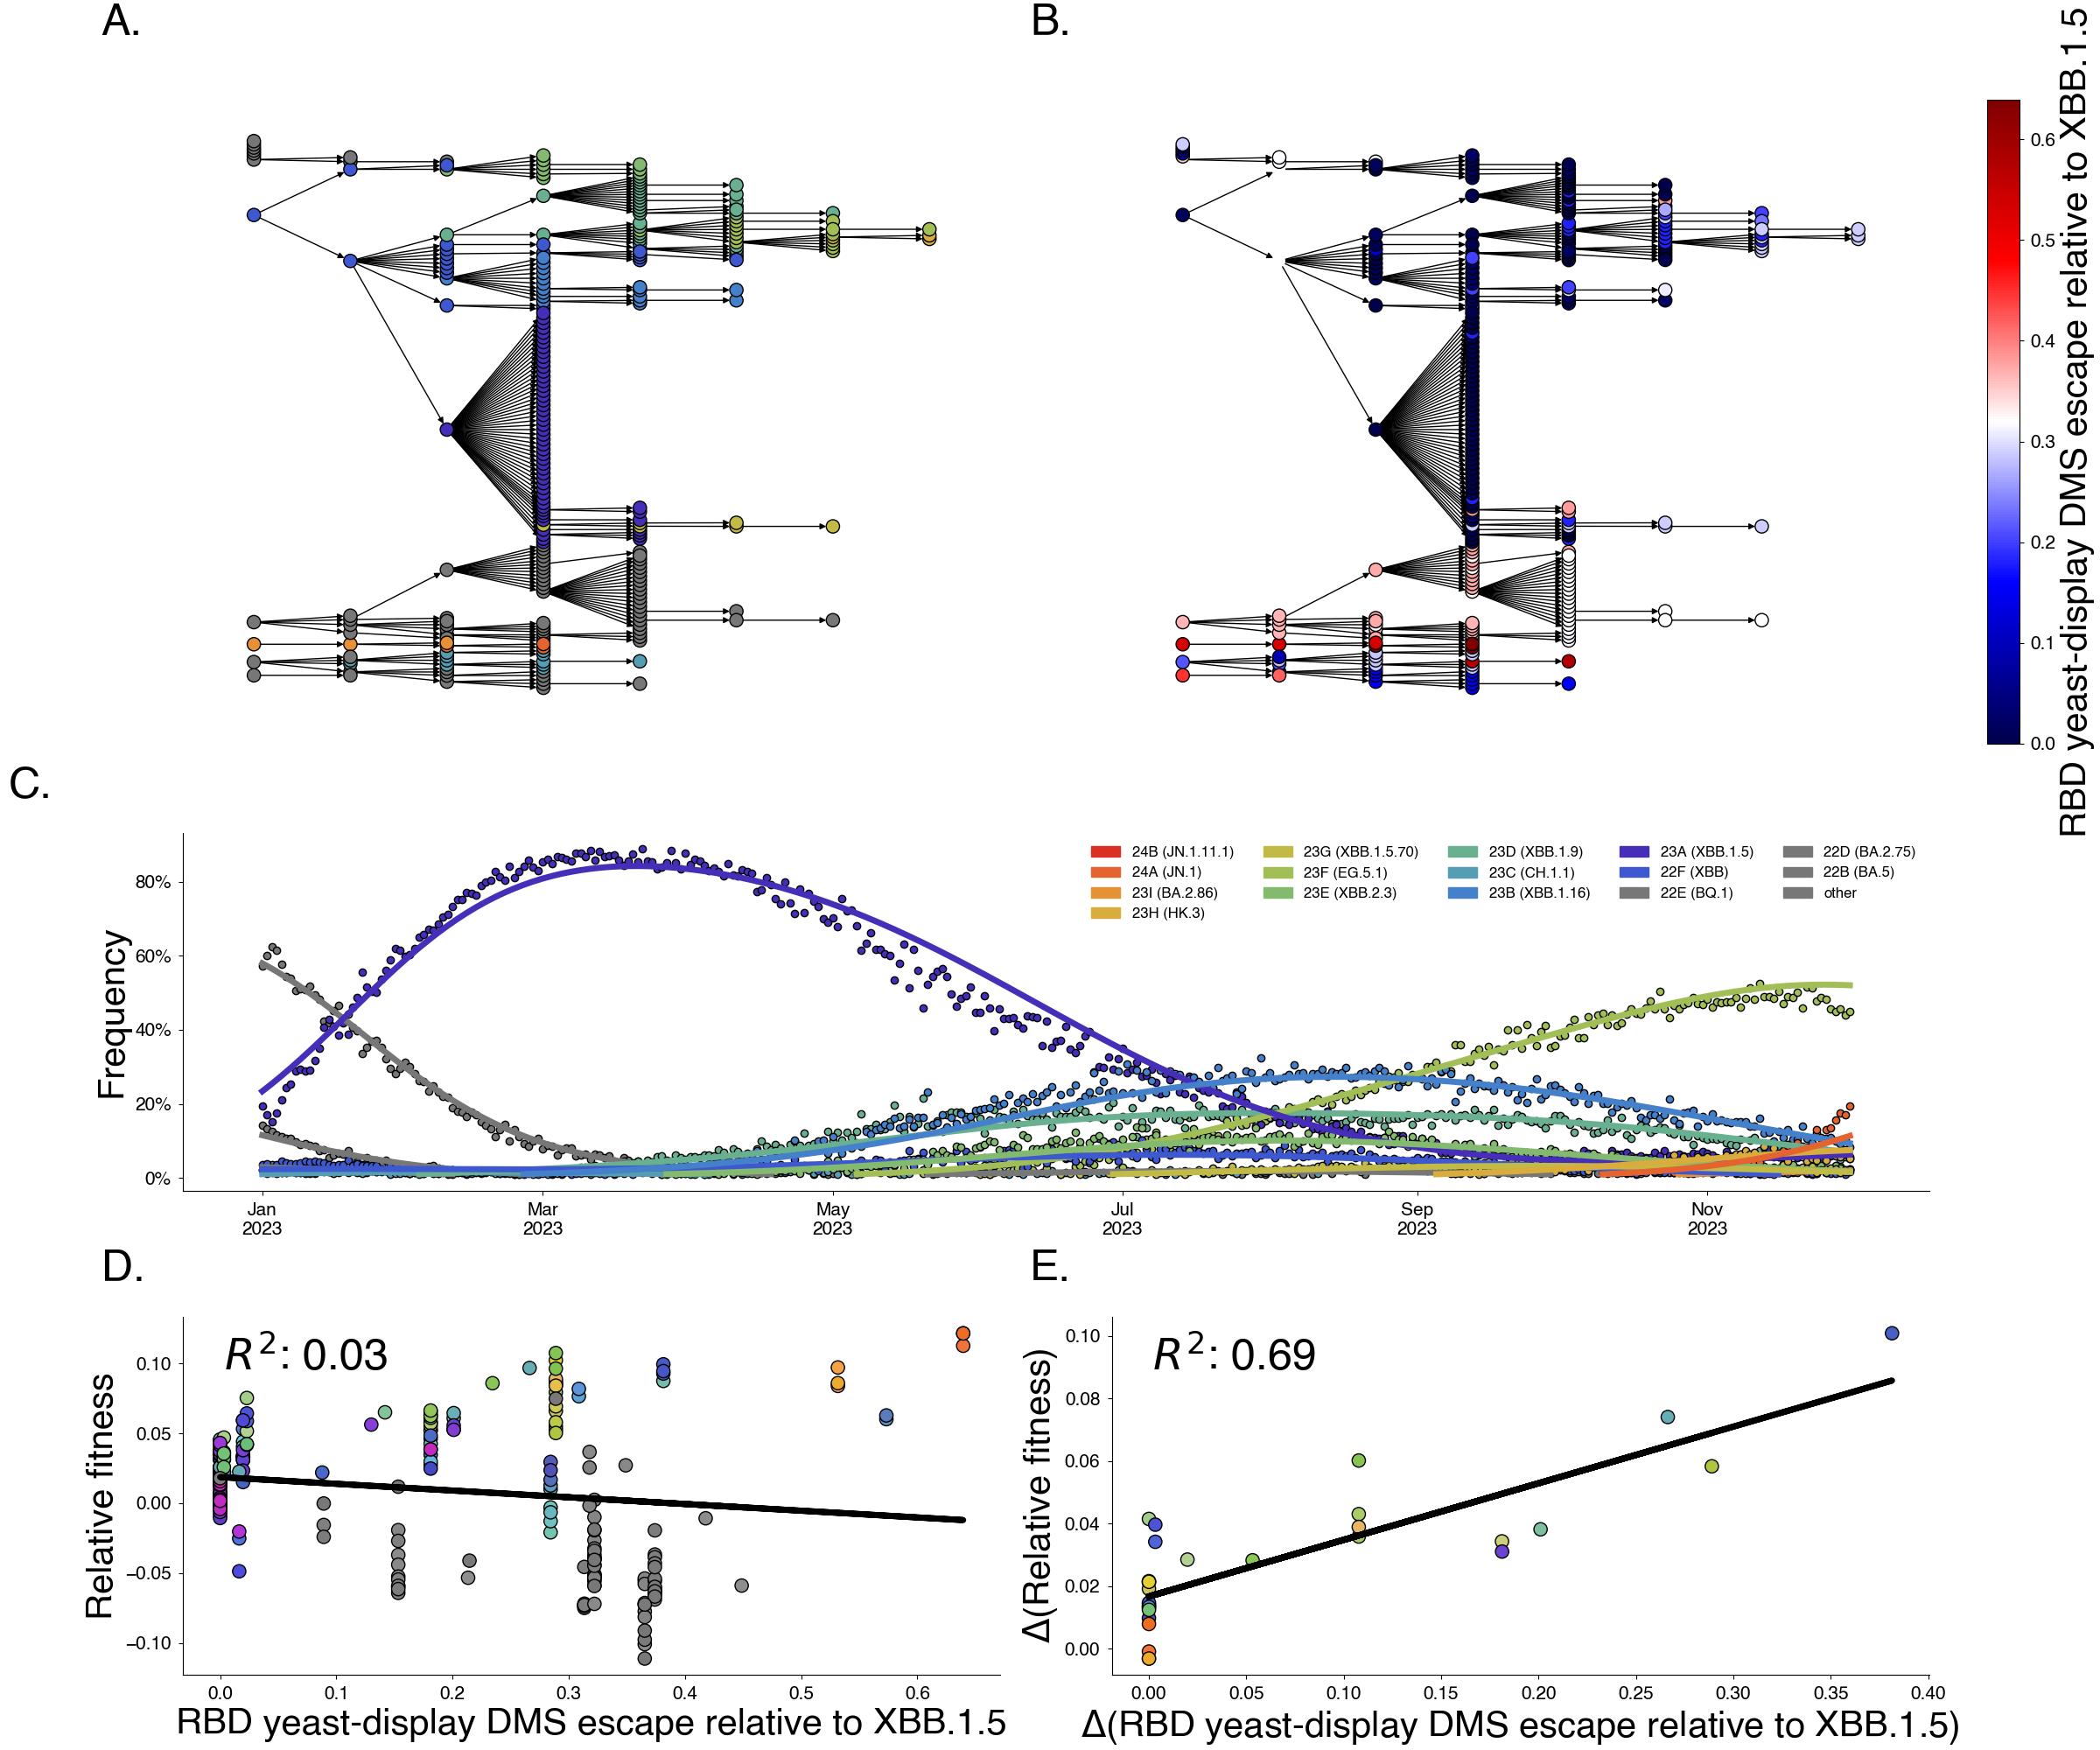
\includegraphics[width=0.9\textwidth]{./figures/interplay_phylo_escape_fitness.png}

    \caption{
	\textbf{Interplay between evolution, immune escape, and fitness among SARS-CoV-2 variants.}
	A. Lineage and closest parent mapping of SARS-CoV-2 Pango lineages, with nodes colored by Nextsrain clade, illustrating evolutionary relationships and grouping of lineages.
	B. The mapping as A., now colored by receptor-binding domain (RBD) immune escape, highlighting molecular phenotypes across evolutionary lineages.
	C. Temporal dynamics of clade frequencies in the global SARS-CoV-2 population from January to November 2023. The figure highlights the rapid turnover of clades driven by changing fitness landscapes.
	D. Naive correlation between RBD immune escape (x-axis) and relative fitness (y-axis) shows weak association ($R^2 = 0.03$), reflecting the confounding effects of shared ancestry.
	E. Innovation-based correlation between immune escape contrasts and fitness innovations shows a significantly stronger relationship ($R^2 = 0.69$), demonstrating the importance of accounting for evolutionary context to uncover true mechanistic drivers of fitness.
    }
    \label{fig:interplay_phylo_escape_fitness}
\end{figure}

\paragraph{Shared evolutionary history generates spurious correlations}

In naive regression methods, cumulative molecular phenotypes, such as immune escape, are directly correlated with measures of fitness.
This naive approach often fails to account for the nested structure and shared evolutionary of lineages which can generate spurious correlations between fitness and phenotype in closely related lineages.

Simulating phylogenetic trees under selection, we show that fitness increases over time as more fit lineages reproduce in the population (Fig.~\ref{fig:shared_history_spurious_correlation}A).
Though we simulate this tree assuming selection is independent of individual mutations or their number, we find that the total number of mutations explains much of the variance in relative fitness ($R^2=0.76$), as shown in Fig.~\ref{fig:shared_history_spurious_correlation}B.
This spurious correlation is due to shared evolutionary history creating correlations between individual lineages in the population despite branch level innovations being independent.
In fact, we can see that the magnitude of the $R^2$ increases with the variation in fitness between branches i.e. the strength of selection in the population (Fig.~\ref{fig:fitness-variation-variance-explained}A).
This suggests that stronger selection amplifies the confounding effect of shared ancestry.

To address this challenge, we focus on fitness innovations i.e. branch-specific changes in relative fitness. 
Using innovations or changes in fitness and mutations across branches within our regressions, we isolate the contributions of molecular phenotypes to fitness, effectively removing the confounding effects of shared ancestry (Fig.~\ref{fig:shared_history_spurious_correlation}C).
This relationship between fitness innovations and mutation change is preserved across varying levels of selection strength (Fig.~\ref{fig:fitness-variation-variance-explained}B).

We show that this approach is similar to other approaches of dealing with confounding due to shared ancestry such as phylogenetic generalized least squares in Supplementary Text~\ref{ssec:pgls}.

Using innovations enables us to better resolve drivers of fitness that are obscured by recent evolutionary history.
By isolating the contributions of molecular phenotypes to fitness, this provides a robust foundation for identifying the specific drivers of relative fitness and improving predictions of lineage success.

\begin{figure}[h]
    \centering
    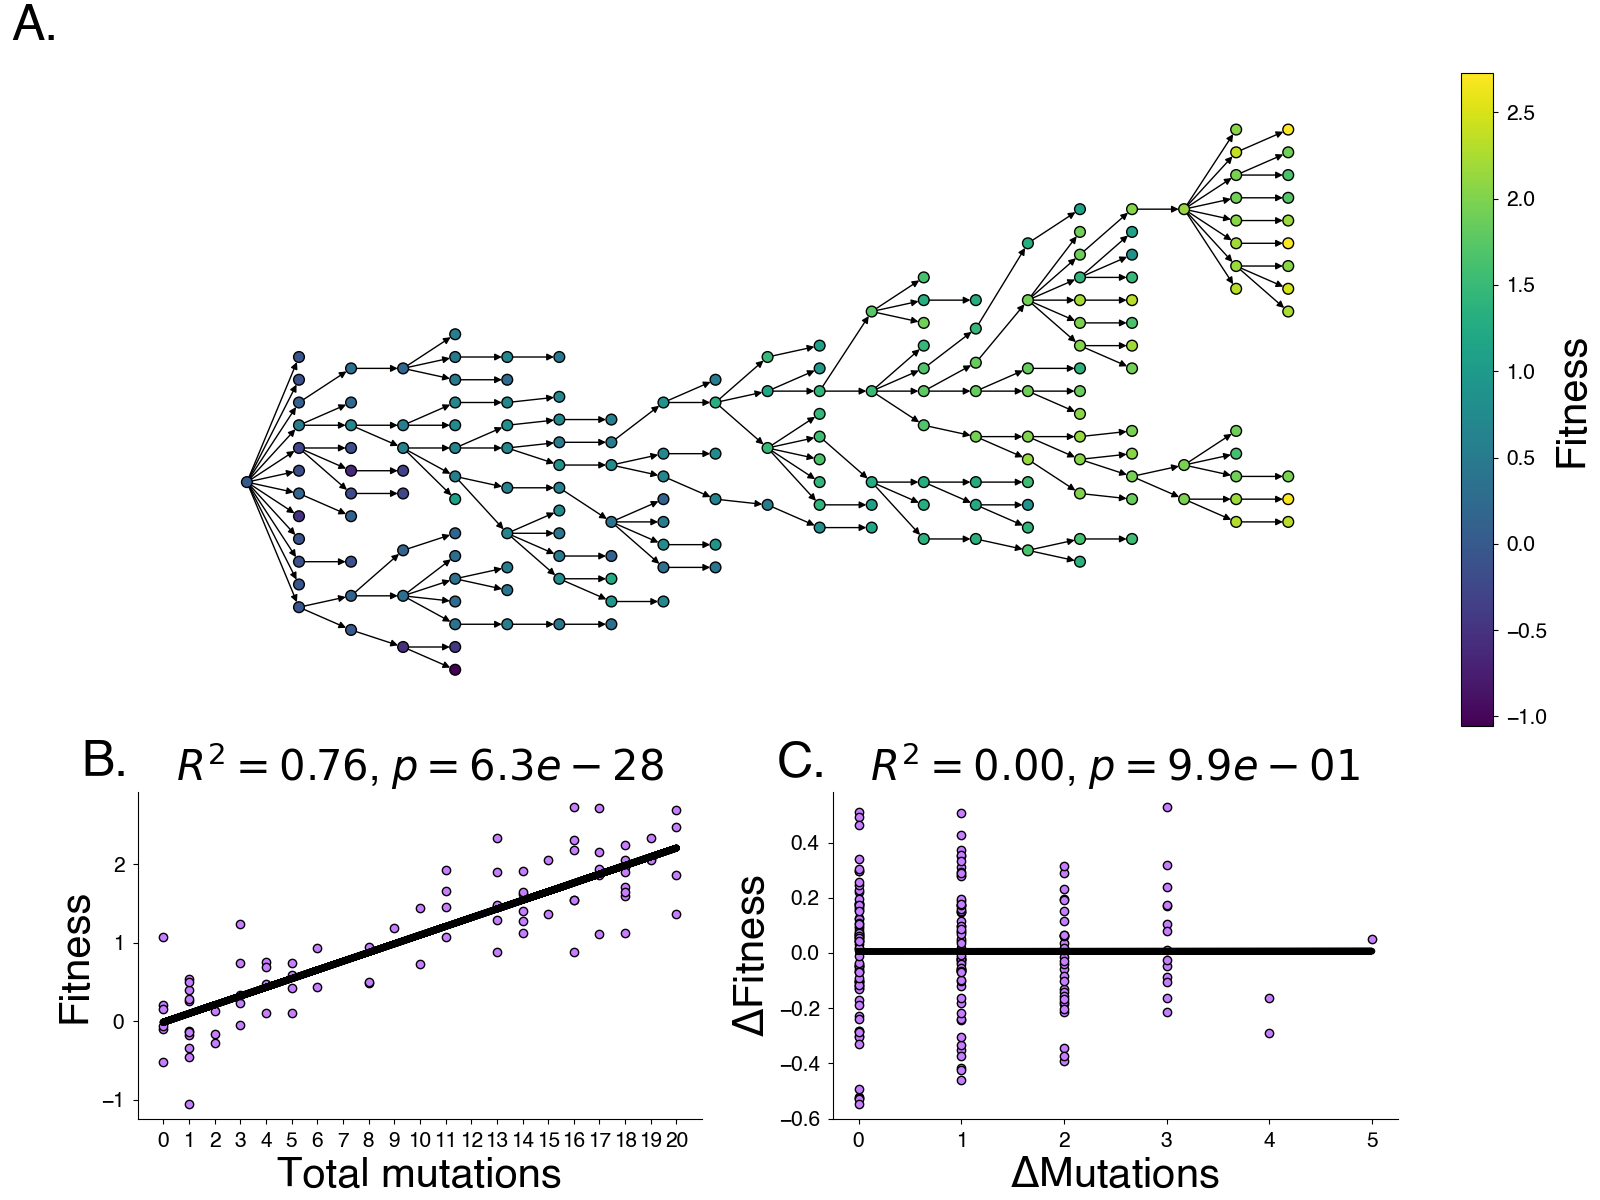
\includegraphics[width=1.0\textwidth]{./figures/synthetic-spurious-correlations.png}
    \caption{
	\textbf{Shared evolutionary history causes spurious correlations between predictors and fitness.}
	A. A phylogenetic tree simulated with fitness-dependent branching.
	Each branch represents the evolutionary descent of lineages, where fitness evolves through Brownian motion.
	B. Naive regression of tip-level fitness on cumulative mutations.
	This ignores the shared evolutionary history of tips, leading to spurious correlations.
	C. Regression of branch-level innovations (changes in fitness versus changes in mutation counts).
	By analyzing innovations, we account for the shared evolutionary history and isolate the relationship between predictors and fitness, revealing the true lack of direct association.
    }
    \label{fig:shared_history_spurious_correlation}
\end{figure}


\paragraph{Estimating fitness innovations across lineages and clades}

To better understand the variability in fitness changes across SARS-CoV-2 lineages, we apply the innovation idea to an inference model nested within a multinomial logistic regression framework.

This innovation model estimates each lineages' fitness relative to XBB.1.5 and its innovation using the lineage-parent mapping in Fig.~\ref{fig:interplay_phylo_escape_fitness}A.

For this analysis, we use a Normal distribution as a prior for the relative fitness innovations.
We fit this model to XBB.1.5-focused dataset spanning January to November 2023, reflecting the evolutionary dynamics during this period and visualize estimated clade frequencies in Fig.~\ref{fig:interplay_phylo_escape_fitness}C, showing turnover in this period.
These clade frequencies are generated by summing the frequency over all Pango lineages within a clade.

In Fig.~\ref{fig:exploring-fitness-innovations}C, we see that there is clear selection for clades like 23F (EG.5.1) and 24A (JN.1).
Despite this, we see that the overall distribution of innovations is near 0, though it has a wide range with a slight positive skew (Fig.~\ref{fig:exploring-fitness-innovations}B).
This reflects the effect of selection in driving advantageous lineages to higher frequencies, but suggests that both adaptive events and neutral evolutionary processes shaped SARS-CoV-2 evolution in this period.

When aggregated by Nextstrain clade, the fitness innovations present a granular view of the evolutionary trends in SARS-CoV-2 (Fig.~\ref{fig:exploring-fitness-innovations}C).
Generally, clades which appear before 23A (XBB.1.5) such as 22B (BA.5) and 22D (BA.2.75) have a median innovation near 0 which is consistent with neutral evolution.
However, clades following 23A (XBB.1.5.) tend to have positive fitness innovations over average, aligning with their observed growth and dominance during this period. 

This analysis shows that fitness innovations can be used to understand patterns of adaptation within a population or clade.
The variability observed across lineages and clades underscores the role of rare but impactful events in driving lineage success and driving outbreaks.

\begin{figure}[h]
	\centering
	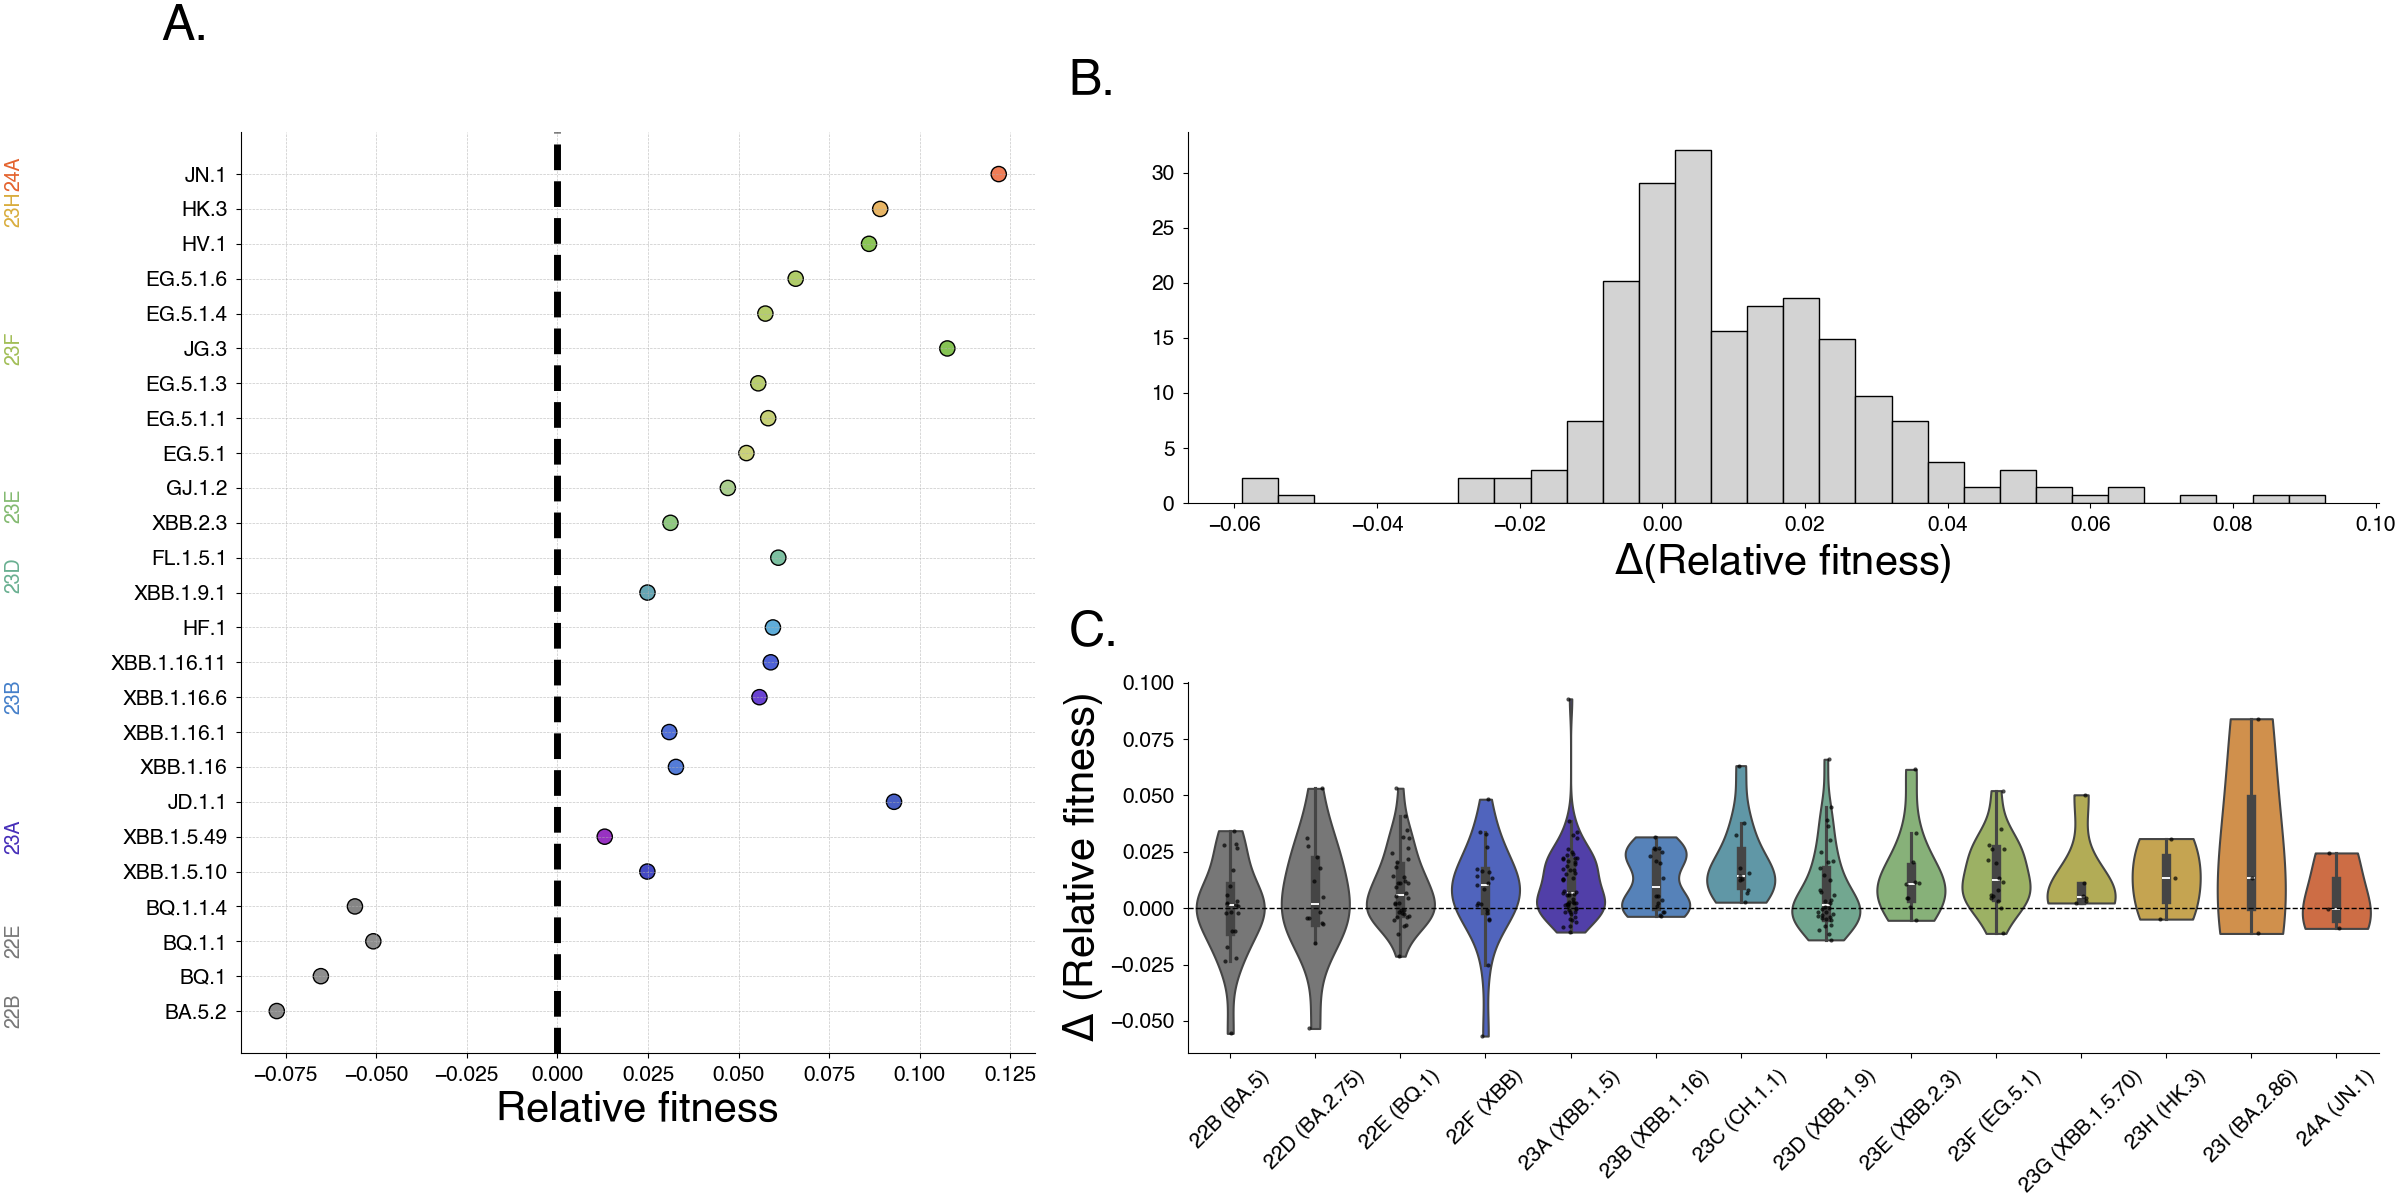
\includegraphics[width=1.0\textwidth]{./figures/exploring-fitness-innovations.png}
	\caption{\textbf{Exploring fitness innovations across SARS-CoV-2 clades.}
	    A. Estimated relative fitness for Pango lineages which reach at least 1\% frequency.
	    B. Histogram of overall fitness innovations across all variants.
	    C. Estimated fitness innovations by clade.
	}
	\label{fig:exploring-fitness-innovations}
\end{figure}

\paragraph{Quantifying the relationship between molecular phenotypes and fitness innovations}

To quantify the relationship between molecular phenotypes and fitness innovations, we integrated deep mutational scanning data to predict lineage phenotypes.

For this analysis, we use ``human sera escape relative to XBB.1.5'' and ``ACE2 binding relative to XBB.1.5'' \cite{Dadonaite2023} and ``RBD ACE2 affinity relative to XBB.1.5'', ``RBD expression relative to XBB.1.5'', ``RBD escape relative to XBB.1.5'' \cite{Taylor2023} as phenotypes.

These phenotypes were calculated for each lineage as the sum of all mutation effects relative to XBB.1.5 and lineage-parent differences in these phenotypes were computed to serve as predictors in the innovation-based analyses.

Using the relative fitness innovations estimated previously (Fig.~\ref{fig:explaining-fitness-innovations}A), we use the changes in these phenotypes across parent-child pairs to predict relative fitness with linear regression.
Together, these phenotypes explain a large share of the variance in relative fitness $(R^2=0.79)$, showing the utility of these phenotypes for predicting changes in relative fitness (Fig.~\ref{fig:explaining-fitness-innovations}B).

To understand the contribution of each of these phenotypes to this regression, we estimated the partial $R^2$ of each phenotype (Fig.~\ref{fig:explaining-fitness-innovations}C).
This is a form of the additional variance explained by adding this phenotype to the model.
Using this partial $R^2$ approach shows that RBD yeast-display escape relative to XBB.1.5 explains most of the variance ($R^2_{\text{partial}} = 0.097$).

%TODO: Mention other phenotypes.
This analysis shows that molecular phenotypes are able to explain much of the variance of fitness innovations within sample.
Among the phenotypes, RBD yeast-display escape relative to XBB.1.5 contributes the largest unique share to the variance. 
This result emphasizes the role of immune escape and its molecular basis in shaping the success of SARS-CoV-2 lineages.

This suggests these molecular phenotypes may have utility for forecasting the relative fitness of previously unseen SARS-CoV-2 lineages.
% To address this, we implemented a regression-based prior for the relative fitness innovation.
% Using this prior, we can sample relative fitness innovations of a lineage given its phenotype and an in-sample parent lineage.
% This enables direct out-of-sample prediction of relative fitness on unseen lineages exploiting phylogenetic structure and molecular data.

\begin{figure}[h]
	\centering
	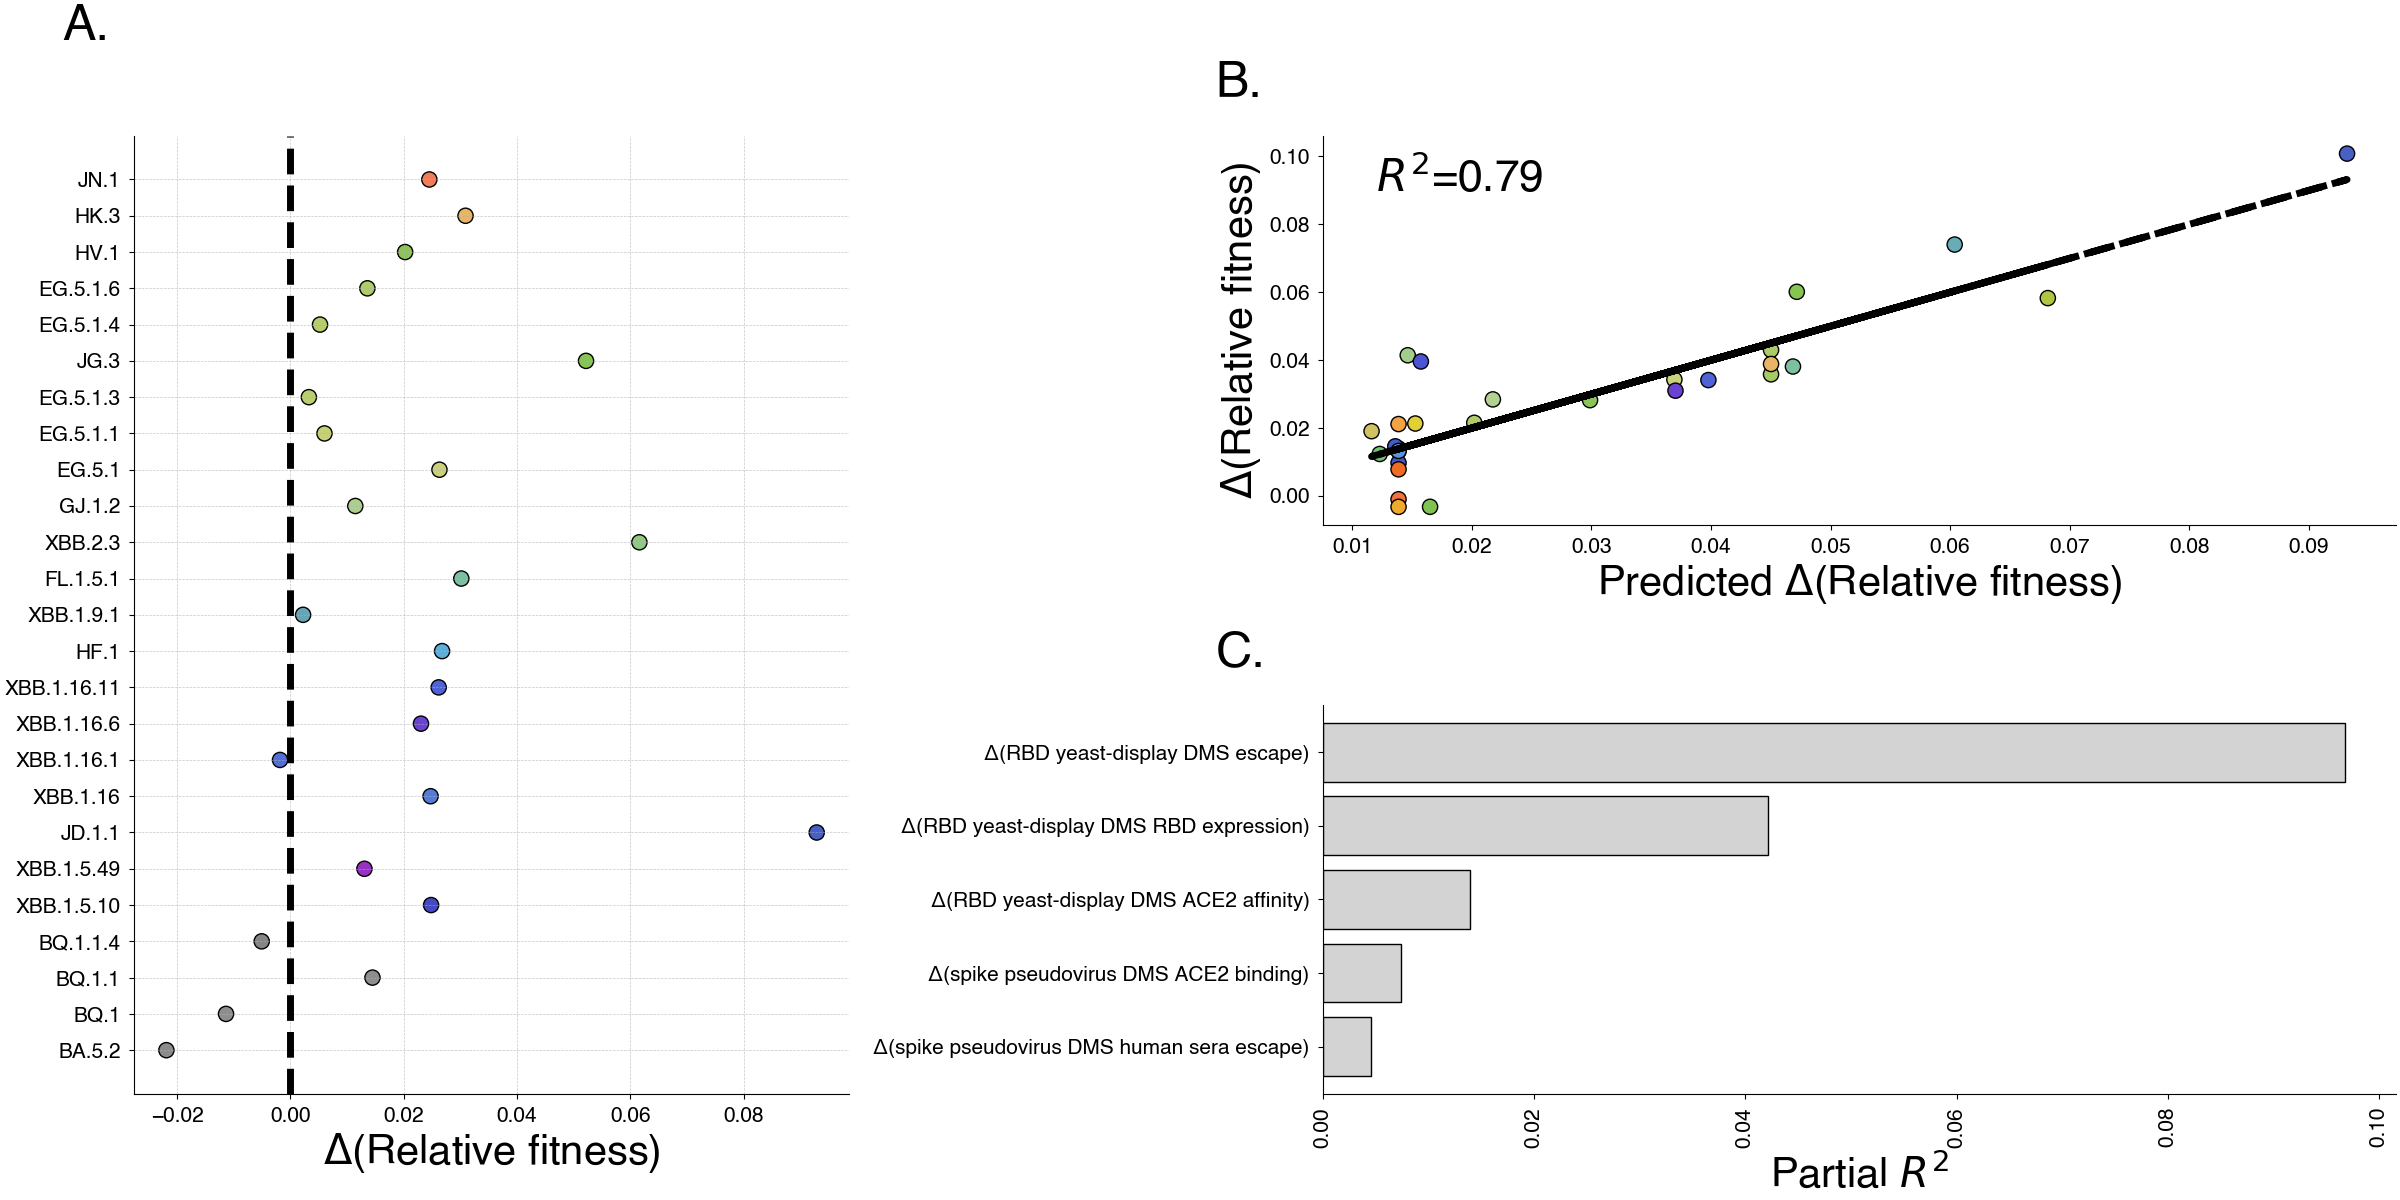
\includegraphics[width=0.95\textwidth]{./figures/explaining-fitness-innovations.png}
	\caption{\textbf{Molecular phenotypes explain fitness innovations.}
	    A. Relative fitness innovations for Pango lineages which reach at least 1\% frequency.
	    B. Observed versus predicted relative fitness innovations from the regression model ($R^2 = 0.72$), demonstrating the model’s predictive accuracy.
	    C. Partial $R^2$ values for molecular predictors, illustrating the relative contributions of features such as immune escape, receptor binding, and expression to fitness innovations.
	}
	\label{fig:explaining-fitness-innovations}
\end{figure}

\paragraph{Using molecular phenotypes for out-of-sample relative fitness forecasts}

To assess the predictive utility of molecular phenotypes, we implemented a regression-based prior for the relative fitness innovation. This approach enables the prediction of fitness innovations for out-of-sample lineages by leveraging their molecular phenotypes and the lineage-parent relationships described previously.
With these predicted fitness innovations, we can then forecast relative fitness using the baseline fitness of its parent (Fig.~\ref{fig:predicting-fitness-with-innovations})

% TODO: Within sample validation

% TODO: Outside sample validation

% Figure~\ref{fig:forecasting-validation}A shows the predicted versus observed fitness innovations for lineages not included in the initial regression model. The predictions align closely with the observed values, demonstrating strong forecasting accuracy with an $R^2$ of 0.72. This result highlights the ability of the regression-based prior to generalize fitness predictions beyond the training set, effectively utilizing molecular phenotypes as predictors.
%
% \paragraph{Validation against observed clade dynamics}
%
% To validate these predictions, we compared the model’s forecasts with observed changes in clade frequencies over time. By aggregating lineage-level predictions to the clade level, we assessed whether the predicted fitness innovations corresponded to observed clade dynamics. Figure~\ref{fig:forecasting-validation}B illustrates the temporal evolution of clade frequencies, with predicted fitness innovations closely tracking the observed growth trajectories of dominant clades such as 23F (EG.5.1) and 24A (JN.1).
%
% These results confirm that the regression-based innovation framework captures key adaptive events driving clade success. Clades with positive fitness innovations showed consistent increases in frequency, while those with negative innovations declined or remained stable. This validation against empirical dynamics demonstrates the robustness of the framework for forecasting evolutionary trajectories.

The ability to predict fitness innovations for previously unseen lineages provides a critical tool for evolutionary forecasting.
By combining molecular phenotypes with the innovation framework, this approach offers a scalable solution for anticipating the success of novel variants in real-time.

% The results presented here highlight the utility of molecular phenotypes and the innovation framework for quantifying and forecasting SARS-CoV-2 fitness innovations.
% This approach is a powerful tool for understanding adaptation and anticipating the potential of emerging variants.
% The implications of these findings, their limitations, and their potential applications to future variant surveillance are explored in the following discussion.

\begin{figure}[h]
	\centering
	% 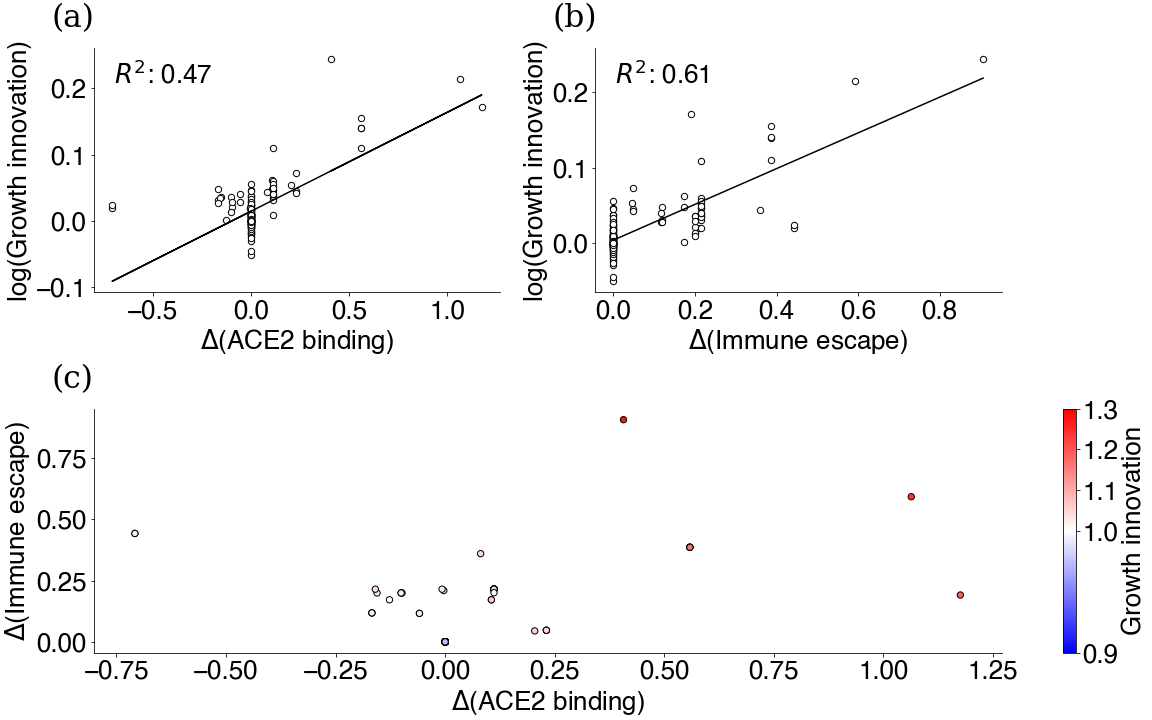
\includegraphics[width=1.0\textwidth]{./figures/binding-escape-score-growth-advantage-innovations.png}
	\caption{\textbf{Predicting fitness with innovations.}
	    A. In-sample validation comparing predicted relative fitness innovations with their estimated values.
	    Predictions were generated using the regression-based prior, incorporating molecular phenotypes as predictors.
	    Points represent individual lineages, with the diagonal dashed line indicating perfect agreement between predicted and estimated values.
	    % The high $R^2$ value demonstrates strong internal consistency, validating the model’s ability to accurately predict fitness innovations for lineages included in the training dataset.
	    B. Out-of-sample validation comparing predicted relative fitness innovations with observed values for lineages not included in the training dataset.
	    % Predictions leverage molecular phenotypes and parent-child relationships to estimate fitness innovations for unseen lineages.
	    % Points represent individual lineages, with the diagonal dashed line indicating perfect agreement. The model achieves an $R^2 = 0.72$, demonstrating robust generalizability to lineages outside the training set.
	    C. Sorted list of lineages with the highest predicted fitness innovations.
	    Lineages are ranked by their predicted relative fitness innovations.
	    % The top-ranking lineages predominantly include descendants of XBB.1.5, with molecular phenotypes suggesting strong immune escape or ACE2 binding affinity. This analysis illustrates the potential of the model to identify high-fitness variants and inform surveillance efforts.
	}
	\label{fig:predicting-fitness-with-innovations}
\end{figure}

% \begin{figure}[h]
% 	\centering
% 	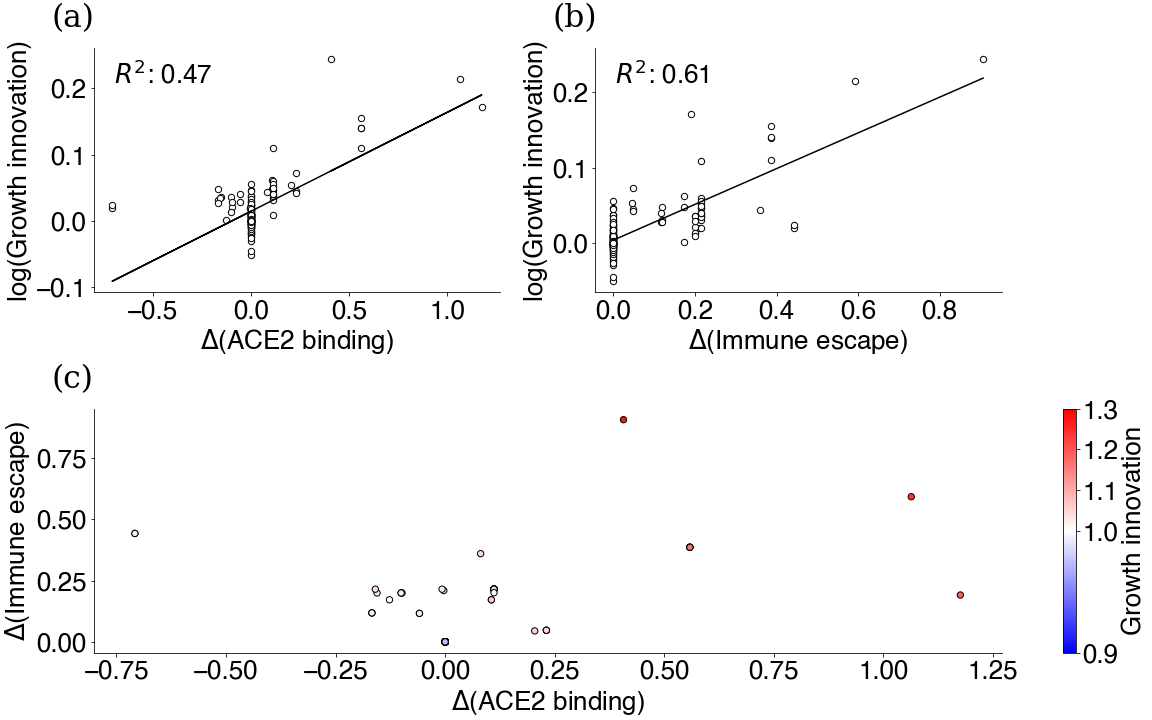
\includegraphics[width=1.0\textwidth]{./figures/binding-escape-score-growth-advantage-innovations.png}
% 	\caption{\textbf{Correlation between changes in ACE-2 binding, immune escape and MLR growth advantage.}
%         A. Correlating log(growth advantage innovation) and change in ACE-2 binding. 
%         B. Correlating SOMETHING and change in immune escape.
%         C. Comparing predicted growth advantage from multiple regression to estimated growth advantage from innovation MLR model.
% 	}
% 	\label{fig:binding-escape-score-growth-advantage-innovations}
% \end{figure}

\section{Discussion}

This study addresses the challenge of predicting the success of unseen variants in rapidly evolving populations.
By integrating molecular phenotypes with relative fitness, we isolate branch-specific fitness innovations while addressing confounding due to shared ancestry.
Our results suggest that molecular phenotypes, particularly immune escape, are strong predictors of lineage success.
Using a regression-based prior, we extend this approach to enable out-of-sample forecasting of relative fitness, providing a scalable, mechanism-informed framework for understanding and predicting the evolutionary success of emerging variants.

Immune escape emerges as the most significant phenotypic driver of relative fitness, aligning with prior studies suggesting weaker neutralization of emerging variants in hosts with past exposure.
Molecular phenotypes such as ACE2 binding affinity and RBD expression, also contribute though to a lesser extent.
These results emphasize that while immune escape is a primary driver, transmissibility-related traits also play a role in shaping lineage success of SARS-CoV-2.

The ability to predict relative fitness for unseen variants has significant public health implications.
Linking molecular phenotypes to relative fitness enables longer-term forecasts of lineage success, which can inform vaccine strain updates by prioritizing high-fitness lineages for monitoring or use as candidate strains before they reach dominance.

% Further, early identification of high-risk variants has significant public health implications.
% Linking molecular phenotypes to relative fitness can provide longer-term forecasts of lineage success and be used to inform vaccine strain updates by selecting high-fitness lineages for monitoring or as candidate strains before they reach dominance.

Despite its strengths, this approach has several limitations.
The focus on genomic data from the United States may restrict the generalizability to regions with different immune landscapes.
For pathogens like influenza which have greater regional diversity, this consideration becomes extremely important.
Additionally, the assumption that molecular phenotypes independently contribute to fitness innovations may oversimplify the interactions between phenotypic traits, which may motivate more complex, data-informed prior models.

Our framework also relies on the quality and relevance of deep mutational scanning data, which may not fully describe immune escape in all populations due to host-specific differences.
While molecular phenotypes derived from deep mutational scanning are powerful, they may not fully capture complex interactions, such as epistasis.
These limitations also suggest future directions for expanding this framework.

Future work can refine this approach by incorporating larger datasets spanning diverse regions and lineages beyond XBB.1.5, enabling evaluation of its generalizability across varying immune landscapes. Testing additional molecular phenotypes may improve prediction accuracy and reveal novel drivers of fitness.

This study establishes a framework for forecasting relative fitness for SARS-CoV-2 using molecular phenotypes.
By showing the utility of these phenotypes for predicting fitness and enabling out-of-sample forecasts, our approach provides a practical tool for real-time monitoring of emerging variants and informing vaccine strain selection. 
While focused on SARS-CoV-2, the framework can be adapted to study other rapidly evolving pathogens, extending its relevance beyond the current pandemic.
These contributions provide a foundation for advancing long-term evolutionary forecasting and guiding proactive responses to pathogen evolution.

% TODO: However this is still a need to update the calculator

% TODO: Epistatis complicates things, might suggest that we need to update phenotype computation


% TODO: However the method remains!

% Our approach bridges mechanistic insights into viral evolution with actionable predictions. 
% Our results show that molecular phenotypes are useful for predicting relative fitness and can enable out-of-sample prediction.
% This ability to forecast fitness for unseen variants offers a practical tool for real-time monitoring of emerging variants and potentially vaccine strain selection.


% The ability to predict relative fitness for unseen lineages represents a significant advancement in evolutionary forecasting.
% This work demonstrates that molecular phenotypes are not only interpretable but also actionable predictors, offering a practical framework for anticipating the emergence of high-fitness variants.
% This approach bridges the gap between mechanistic insights into viral evolution and forecasting tools for public health.

% This approach also depends on the availability and accuracy of deep mutational scanning data.
% If the human sera used in these experimental approaches are not available or reflective of the population of interest, predictors of immune escape may not properly reflect escape risk within our population.


\section{Methods}

\paragraph{Simulation of Phylogenetic Trees with Fitness-Weighted Offspring}%

To investigate how evolutionary history influences correlations between molecular phenotypes and fitness, we simulated phylogenetic trees using a discrete-generation model.
Each tree begins with a single ancestral lineage at generation 0, initialized with fitness $\lambda_0$.
At each generation $t$, the total number of offspring $O_{t}$ is sampled from a Poisson distribution with mean $bar{N}_t$.
These offspring are then distributed among active lineages $i$ are allocated using a multinomial draw based on fitness-weighted probabilities, so that the offspring by lineage are given by:

\begin{align*}
    O_{i, t} &\sim \text{Multinomial}\left(O_t, p_{i}\right),\\
    p_i &= \frac{\exp(\lambda_i)}{\sum_j \exp(\lambda_j)},
\end{align*}
where $\lambda_i$ is the fitness of lineage $i$.
We assume that the fitness of each offspring evolves from its parent’s fitness according to a Brownian motion process
\begin{equation*}
    \lambda_{\text{offspring}} = \lambda_{\text{parent}} + \psi, \quad \psi \sim \text{Normal}(0, \sigma^2),
\end{equation*}
where $\sigma$ determines the variance in fitness evolution.
Mutations accumulate along branches with their counts drawn from a Poisson distribution with rate $\mu$.

The simulation is run over a fixed number of generations, producing trees where fitness influences both branching structure and phenotype evolution.
These trees are then analyzed to compare naive tip-level regressions with branch-level contrast regressions, providing insight into how shared evolutionary history drives spurious correlations and demonstrating the importance of evolutionary-aware statistical approaches.

\paragraph{Generating sequence counts}%

We prepared sequence count data sets using the Nextstrain-curated SARS-CoV-2 sequence metadata \cite{Hadfield2018} which is created using the GISAID EpiCoV database \cite{khare2021gisaid}.
These sequences were counted according to their annotated Pango lineage \cite{aksamentov2021nextclade}, country of collection, and date of collection to produce sequence counts for each variant, date, and country analyzed.

\paragraph{Multinomial logistic growth}

To estimate relative rates of growth between variants of interest, we fit a multinomial logistic growth model to the sequence count data.
This model can be written as:
\begin{align*}
    f_{t, v} = \frac{\exp(\alpha_{v} + \lambda_{v} t)}{\sum_{u=1}^{V} \exp(\alpha_{u} + \lambda_{u} t)},
\end{align*}
where $\alpha_{V} = \lambda_{V} = 0$.

We can then interpret $\lambda_{v}$ as the relative fitness of variant $v$ relative to variant $V$.
Assuming a fixed generation time $\tau$ additionally allows us to then write the relative $R_{t}$ or growth advantage for variant $v$ over $V$ as $\Delta_{v} = \exp(\lambda_{v}\tau)$.
To fit this model, we use a multinomial likelihood with probabilities defined by the frequencies above, the vector of counts for each variant at time $t$ $S_{t}$, and the total count of sequences at time $t$:

\begin{align*}
    S_{t} \sim \text{Multinomial}(N_{t}, f_{t, \cdot}).
\end{align*}

\paragraph{Mapping variant-parent relationships}%

In order to estimate rough branch-specific relative fitness innovations, we develop a data set mapping variants as parent-child pairs.
For each Pango lineage in our generated sequence counts, we iterate to its parent lineage until the parent lineage is either in the sequence count file or there is no parent present.
If there is no parent present, we simply estimate the variant's relative fitness and growth advantage directly.

\paragraph{Relative fitness innovation model}%

We can extend the previous model for the Multinomial Logistic growth to take into account for evolutionary relationships using the variant-parent lineage mapping generated in the previous section.

This updated model is instead parameterized by the relative fitness difference between variant $v$ and its parent lineages $\psi_{v} = \lambda_{v} - \lambda_{\text{parent}_{v}}$ directly.
Under this parameterization, we can also define the (approximate) growth advantage innovations $\Psi_{v}$ from a variant lineage $v$ to its parent as:
\begin{align*}
\Psi_{v} = \frac{\Delta_{v}}{\Delta_{\text{parent}_{v}}} = \exp(\psi_{v} \tau).
\end{align*}

\paragraph{Normal prior model}%

We consider several prior models on the relative fitness innovation $\psi_{v}$.
The most basic of this model is a normal prior:
\begin{align*}
    \psi_{v} = (\lambda_{v} - \lambda_{\text{parent}_{v}}) \sim \text{Normal}(0, \sigma).
\end{align*}

This induces a log normal prior on the growth advantage innovations $\Psi_{v}$.

\paragraph{Regression prior for growth advantage innovations}%

To better explain the variation in relative fitness innovations and enable prediction of relative fitness for new variants given features and their parent lineage, we extend the above prior to be parameterized by various features, so that
\begin{equation}\label{eq:relative_fitness_regression}
    \psi_{v} = (\lambda_{v} - \lambda_{\text{parent}_{v}}) \sim \text{Normal} \left( \sum_{p} \theta_{p} x_{p}, \sigma \right).
\end{equation}

Using this model, we can then predict relative fitnesses and growth advantages out of sample.
For a given out-of-sample variant $v$, we need to only specify its set of predictors $x_{p}$ and its in-sample parent $\text{parent}_v$.
First, we predict its innovation relative to its parent and its total relative fitness by sampling using Equation \ref{eq:relative_fitness_regression} with the estimated $\theta_{p}$.
We can compute the relative fitness of this variant by adding the predicted innovation to the estimated relative fitness of its parent.
This provides an out-of-sample estimate of the relative fitness using a combination of molecular data and our knowledge of the evolutionary history of the population.

% \paragraph{Extending to time-varying growth advantage innovations}%
%
% \begin{align*}
%     \psi_{v,t} &= (\lambda_{v,t} - \lambda_{\text{parent}_{v}, t}) \sim \text{Normal} \left( \sum_{p} \beta_{p} x_{p}, \sigma \right) \\
%     \beta_{p, \cdot} &\sim \text{RandomWalk}(0, \gamma)
% \end{align*}

\paragraph{Generating features for regression prior analysis}%

% TODO: Explain what deep mutational scanning and why RBD is relevant
We use mutation effects estimated using pseudovirus deep mutational scanning and receptor binding domain (RBD) yeast-display deep mutational scanning to predict phenotypes at the level of Pango lineage \cite{Dadonaite2023, Taylor2023}.
The phenotype of each lineage is computed as the sum of all mutation effects relative to XBB.1.5.
This gives us 5 molecular phenotypes: ``spike pseudovirus DMS human sera escape relative to XBB.1.5'', ``spike pseudovirus DMS ACE2 binding relative to XBB.1.5'', ``RBD yeast-display DMS ACE2 affinity relative to XBB.1.5'', ``RBD yeast-display DMS RBD expression relative to XBB.1.'', ``RBD yeast-display DMS escape relative to XBB.1.5''.

We also compute the variant-parent differences in the phenotypes for use as predictors in the innovation-based analyses. 
These variant-parent differences are computed using the variant-parent relationships described above for variants with an existing parent.

\paragraph{Analysing SARS-CoV-2 evolution post-XBB.1.5 emergence.}

To analyze selection in SARS-CoV-2 after the emergence of XBB.1.5, we begin by generating Pango lineage-level sequence counts for the United States between January 1st, 2023 and December 1st, 2023. 
We collapse small lineages which do not meet a count threshold into their parent lineages, forcibly including XBB, XBB.1.5, and XBB.2.
Using these collapsed counts, we generate the variant-parent relationships.
We, then, estimate the relative fitness of each variant and its innovation using these sequence counts and the innovation model with a normal prior on the innovations.

Using these estimated innovations, we fit a standard linear regression between the relative fitness innovation and the molecular phenotype innovations.
To evaluate the contribution of adding individual phenotypes to the relative fitness innovations, we conducted a partial $R^2$ analysis.
We compute the partial $R^2$ for each phenotype as the difference between the $R^2$ of the full model and the $R^2$ of the model without the phenotype of interest.
This approach quantifies the proportion of variance in the dependent variable (relative fitness innovation) explained by each phenotype when adding it to a model that already uses the other phenotypes.

We also estimate the relative fitness of each variant and its innovation to its parent using the regression prior on the innovations with the 5 molecular phenotypes as predictors.
This enables us to make predictors of the phenotype for out of sample lineages as long as we know their parent and their phenotypes.

\subsection*{Acknowledgements}

We gratefully acknowledge all data contributors, i.e. the Authors and their Originating laboratories responsible for obtaining the specimens, and their Submitting laboratories for generating the genetic sequence and metadata and sharing via the GISAID Initiative, on which this research is based.

\subsubsection*{Funding}

This work is supported by NIH NIGMS award R35 GM119774 to TB and a Howard Hughes Medical Institute COVID-19 Collaboration Initiative award to TB.
MF is an ARCS Foundation scholar and was supported by the National Science Foundation Graduate Research Fellowship Program under grant No.\ DGE1762114.
TB is a Howard Hughes Medical Institute Investigator.

\subsubsection*{Competing interests}

All authors declare no competing interests.

\subsubsection*{Data and materials availability}

Molecular phenotype data was provisioned from \href{https://github.com/jbloomlab/SARS2-spike-predictor-phenos}{https://github.com/jbloomlab/SARS2-spike-predictor-phenos} on November 24, 2024.
Sequence data including date and location of collection as well as clade annotation was obtained via the Nextstrain-curated data set that pulls data from GISAID database.
A full list of sequences analyzed with accession numbers, derived data of sequence counts and molecular phenotypes, along with all source code used to analyze this data and produce figures is available via the GitHub repository \href{https://github.com/blab/ncov-escape}{github.com/blab/ncov-escape}.


% ========== Chapter 6
\graphicspath{{./chapters/operationalizing-forecasts/}}
\chapter{Operationalizing evolutionary forecasts: \evofr\ and \forecastsNcov}

In this chapter, we develop and discuss two software tools \evofr\ and \forecastsNcov\ that simplify the development, application, and communication of variant fitness dynamics and evolutionary forecasts.

\section{Introduction}

This dissertation emphasizes integrating theoretical and practical approaches and blending mechanistic insights with statistical models.
While earlier chapters focused on developing, evaluating, and applying specific models, these methods were used in specific analyses motivated by existing scientific problems.
However, there is a common structure in the methods described that enables us to simplify the workflow of using these kinds of models.
In this way, we move from scientific analyses to reproducible, scalable, and applied analyses that can tackle broad questions in evolutionary forecasting. % TODO: Addressing real-time analysis
Having infrastructure for building, applying, and interpreting models allows us to iterate on our analyses, speeding up our responses and addressing real-world challenges.

% TODO: We should talk about the interest in understanding global trends for vaccine strain selection, for variant classification, and monitoring

%TODO: Expand on what it means to operationalize

\evofr\ consolidates and expands on the methods developed in this dissertation, enabling reproducible data analysis within a modular structure that allows rapid testing and comparison between models. %TODO: Reframe.
This package serves as the computational backbone for the analyses presented in this dissertation, integrating models from statistical tracking to mechanistic forecasting and is the bridge between the theoretical insights developed in this dissertation and their practical utility as an open-source tool. 

\forecastsNcov\ incorporates \evofr\ into an automated workflow and public-facing platform, translating research and applied forecasts into actionable insights for public consumption.
It continually retrieves publicly available sequence data to generate and visualize forecasts of SARS-CoV-2 variant frequencies for public consumption, providing forward-looking approach to the evolution of SARS-CoV-2 as a companion to Nextstrain. \cite{Hadfield2018}
In this way, \forecastsNcov\ serves as a first step to operationalized evolutionary forecasting in practice and at scale.

Together, these software tools provide a basis for evolutionary forecasts as a dynamic process and concrete problem, setting the stage for continued development of this practice and scientifically-informed forecasts of pathogen evolution.

\section{\evofr: A toolkit for evolutionary forecasting}

Evolutionary forecasting plays a critical role in understanding genetic changes in populations over time, with direct applications in predicting the prevalence of infectious disease variants, guiding vaccine development, and informing public health interventions.

Existing tools for understanding evolution often operate at the level of phylogenetic tree estimation which is computationally expensive due to the large number of possible trees (which grows super-exponentially in terms of the number of samples).
Further, these methods have shown difficulty scaling to large numbers of sequences, requiring approximation-based methods at the pandemic scale. \cite{DeMaio2023}
Additionally, due to these large computational demands, it can be difficult to iterate on these methods, making model development, testing, and iteration time-consuming.
In general, these methods are typically employed for historical analyses, capturing past or currents trends in evolution without much concern for likely future population change.
That being said, there is no need to completely replace phylogenetic analysis as it still forms an important backbone for our understanding of pathogen evolution and enables us to group continuous genetic diversity in pathogen populations to variant groupings that are evolutionarily meaningful.
%TODO: What do I cite here.

This suggests a need to supplement phylogenetic analysis with fast, scalable, reproducible methods for analyzing sequence data at a coarse scale that can be employed for both historical and forward-looking analyses.
To address these gaps, we have developed \evofr.

\evofr\ is a Python package built for evolutionary forecasting of genetic variants, addressing the growing need for robust tools to analyze and predict change in genetic variation in real time.
With applications in evolutionary biology, epidemiology, and public health, \evofr\ integrates data pre-processing, modeling techniques, intuitive visualization tools, and a modular framework to empower researchers and scientists to understand and anticipate the dynamics of genetic variation.
It seeks to simplify bespoke analyses and allow easy integration in standardized workflows, enabling reproducible and scalable analyses.

The package facilitates data preprocessing, evolutionary forecasting, and result visualization, catering to complex datasets like those generated by genomic surveillance of pathogens (e.g., SARS-CoV-2 and influenza). 
By leveraging modularity, \evofr\ ensures scalability and extensibility, enabling users to adapt the tool for varied biological and computational challenges. 
The key contributions of this package include:
\begin{itemize}
	\item \textbf{Forecasting dynamics of genetic variants}: \evofr\ allows users to estimate the relative fitness and future prevalence of genetic variants using customizable modeling approaches such multinomial logistic regression (MLR), renewal-equation based models, Gaussian processes, and latent factor models among others.
	% \item \textbf{Bridging Data and Decision-making}:
	% 	\evofr provides researchers and decision-makers with clear, actionable visualizations of evolutionary dynamics to inform policy and intervention strategies.
	\item \textbf{Extensibility and Accessibility:} \evofr\ provides a user-friendly, open-source framework that integrates seamlessly with Python’s ecosystem, encouraging contributions and customization.
	\item \textbf{Modularity and Reproducibility} \evofr\ promotes reproducible science by offering a modular architecture that supports continued methods development, rapid iteration, model comparison, and simple integration into forecasting workflows.
\end{itemize}

\subsection{Design and implementation}

The design and implementation of \evofr\ reflect its dual purpose as a research product and public health tool.
This section will describe the software's architecture and key features, highlighting its modular design, integration of diverse modeling approaches, interchangable inference methods.

\paragraph{Modularity}

\evofr\ is divided into distinct modules for data preprocessing (\texttt{evofr.data}), modeling (\texttt{evofr.models}), inference (\texttt{evofr.infer}), and visualization (\texttt{evofr.plotting}).
Each module performs specific tasks and is designed to be interoperable.
As an example, this enables easily swapping between different models such as standard MLR, a Gaussian process-based model on the same pre-processed data.
These models can then be fit with any of the inference methods in \texttt{evofr.infer} such as Markov Chain Monte Carlo (MCMC), Stochastic Variational Inference (SVI), and maximum a posteriori (MAP) estimation.
The results of these models are stored in a standardized \texttt{evofr.posterior} object, which is compatible with the various plotting methods stored in \texttt{evofr.plotting}.

\paragraph{Reproducibility}

%TODO: Deterministic workflows, documentation, standardized outputs
Fundamentally, \evofr\ seeks to make the kind of bespoke analyses that are common in papers about SARS-CoV-2 and pathogen evolution reproducible.
It contains well-documented reproductions of several methods employed in research papers, to improve the reach of these methods and enable easy replication of analyses with these papers.

While inference for these models typically involve stochastic processes, \evofr\ includes mechanisms to fix random seeds, ensuring that results are deterministic and consistent across runs.

Additionally, all intermediates and outputs including preprocessed data, model configurations and posterior samples can be stored in standardized formats like JSON and CSV.
This ensures that results can be reliably reproduced and shared.

\paragraph{Extensibility}

Users can extend \evofr\ by adding new models, likelihoods, or priors to the models module by developing a class that inherits from \texttt{evofr.ModelSpec}.
The package’s backend-agnostic design ensures compatibility with diverse computational frameworks (e.g., JAX, PyMC, NumPyro) since users can simply provide a log-posterior probability function for their model to enable samplng or optimization via \evofr's inference methods. \cite{jax2018github, AbrilPla2023, phan2019composable}

The plotting module (\texttt{evofr.plotting}) is built on top of matplotlib, but can be customized or replaced to accommodate specific visualization needs, such as alternative plot styles or integration with external tools. \cite{Hunter2007}

Generally, the open-source nature of \evofr\ encourages contributions, enabling the tool to evolve with user-driven innovations.

\paragraph{Scalability}

Due to most models working at the level of variant frequency, \evofr\ is designed to process genomic datasets containing thousands of sequences, with methods typically scaling with the number of variants and time-horizon for analysis.
Efficient use of computational resources and data reduction strategies ensures that analyses remain feasible as data volumes grow.
Further, integration with JAX enables just-in-time compilation and GPU/TPU acceleration for computationally intensive tasks.

\subsection{Discussion}

% State of evofr
\evofr\ is a Python-based toolkit designed to address challenges in evolutionary forecasting.
Its modular structure and emphasis on flexible workflows enable researchers to analyze and predict genetic variant dynamics.
\evofr\ is well-suited for genomic datasets generated by real-time surveillance efforts, where understanding variant dynamics is essential for public health decision-making and evolutionary monitoring.

Through its modular design, \evofr\ supports rapid iteration on models and analyses, offering tools for data preprocessing, modeling, inference, and visualization. 
By enabling reproducible workflows and fostering extensibility, \evofr\ has the potential to serve a broad range of applications, from fundamental research to forecasting in practice.

% What does evofr do
The core contributions of \evofr\ include the wide range models implemented within the package, which provide a robust foundation for exploring genetic variant dynamics under both statistical and semi-mechanistic frameworks.
By supporting customizable likelihoods and priors, \evofr\ also allows users to tailor models to specific research questions or datasets.

The package is designed to handle large genomic datasets efficiently, ensuring that \evofr\ can be applied to datasets with hundreds of thousands of sequences and extended time horizons at the national and global scale, making it ideal for real-time evolutionary forecasting.

Additionally, \evofr\ enables reproducible workflows with logging model configurations, and storing results in common formats.
These features ensure that analyses can be reliably reproduced, shared, and extended.

% Limitations 
While \evofr\ provides many significant advantages, there are some points of limitation as is.
Bayesian inference methods such as MCMC can demand significant computational resources, especially when dealing with large data sets and complex models.
  Though there are alternative, faster but approximate methods for inference such as stochastic variational inference and maximum a posteriori estimation available within the package, this still remains an issue since all inference methods may not be computational feasible for a given data set or model.

In general, the accuracy of these methods depends heavily on the quality and completeness of the data set of interest.
This means that unforeseen biases or gaps in the data can affect the reliability of these models and their predictions.
However, \evofr's extensibility will allow motivated researchers to iterate on these models to improve their ability to address such data issues.

This level of extensibility presents a potentially steep learning curve. 
Users with limited experience in probabilistic modeling may face challenges using and extended this package as is, but the documentation should provide a helpful guide for contributions looking to dive deeper.

% Future directions
In the future, we hope to expand the capabilities of \evofr\ and address the aforementioned limitations.
Further development should continue to design and implement hybrid models which combine mechanistic insight and statistical flexibility, expanding the range of questions and forms of data that \evofr\ can address and handle.
This includes additional likelihood functions and priors for extending existing models as well.

There is also a need to support contributions to \evofr\ from the open-source community.
This includes adding more thorough documentation of the package as well as the development of extended guide for contributors that is accessible to users.
Going forward, the goal should be expanding the package to meet the needs of the communities who would most benefit from it: researchers and scientists in epidemiology, evolutionary biology, and public health.

% Broader impacts
\evofr\ democratizes evolutionary forecasting by turning statistical methods developed for research to a practical, scalable, and accessible tools for analysis.
This positions \evofr\ as a useful for real-time applications in public, such as monitoring emerging variants or informing vaccine development.

Beyond its immediate applications, \evofr\ serves as a model for the development of modular, extensible tools in computational biology.
Its design and implementation demonstrate the utility of combining reproducibility, scalability, and user-centered design to address complex challenges in research. 
By bridging the gap between theoretical models and practical applications, \evofr\ sets the stage for continued advancements in evolutionary forecasting and beyond.

\subsection*{Code availability}

\evofr\ is an open source project.
Its source code can be found at \href{https://github.com/blab/evofr}{https://github.com/blab/evofr}.
Its documentation can be found at \href{https://blab.github.io/evofr}{https://blab.github.io/evofr}.

\section{\forecastsNcov: Automated and public-facing forecasts for SARS-CoV-2}


\forecastsNcov\ is an automated platform designed to provide real-time forecasts of SARS-CoV-2 variant frequencies.
As part of the broader Nextstrain project, it extends Nextstrain’s genomic surveillance capabilities by offering a forward-looking perspective. \cite{Hadfield2018}
While Nextstrain’s phylogenetic inference provides detailed reconstructions of evolutionary histories, \forecastsNcov\ complements this by projecting future variant trajectories.
This dual approach ensures a comprehensive understanding of variant dynamics, bridging retrospective insights with predictive capabilities.

This tool operationalizes evolutionary forecasting, translating genomic data into actionable insights for public health.
Its automated workflows, robust modeling framework, and accessible visualization tools make it an essential resource for addressing rapidly evolving public health challenges.
By enabling real-time forecasting, \forecastsNcov\ can support early detection of emerging threats, timely policy decisions, and informed vaccine updates.

% \forecastsNcov\ is an automated workflow that processes SARS-CoV-2 sequence data, processes these into a sharable format, applies \evofr’s forecasting models, and visualizes their results in a web interface, providing real-time insights into SARS-CoV-2 variant dynamics.
% \forecastsNcov\ uses publicly submitted genomic data, to produce variant frequency forecasts and variant-specific growth advantages to monitor and nowcast SARS-CoV-2 variant dynamics, directly complementing Nextstrain’s phylogenetic analyses by adding predictive, forward-looking insights.
% \forecastsNcov\ forecasts variant trajectories (e.g., growth advantage, frequency) alongside phylogenetic data from Nextstrain to provide a comprehensive view of virus evolution. This strengthens Nextstrain’s ability to not only visualize past evolutionary relationships but also predict future trends in variant dynamics. %TODO: Correct this heavily. We want to describe this as a frequency-based complement to 

% \forecastsNcov enhances this by predicting the future dynamics of viral variants based on their evolutionary and fitness characteristics.
% While Nextstrain focuses on tracking past evolutionary trends, \forecastsNcov\ looks forward, using statistical and mechanistic models to forecast how variants will evolve over time.

%TODO: Add Figures: Clade level frequencies and growth advantages, lineage growth advantages
% Be sure to caption data last updated

% TODO: Why it's useful for these things to be integrated 
\subsection{Design and workflow}

The \forecastsNcov\ pipeline integrates data ingestion, predictive modeling, and visualization into a seamless, automated workflow.
It is designed to operate at scale, updating forecasts daily to provide consistent and timely insights.

% This is where we discuss automated sequence count generation, the workflow for country-level fitness at multiple levels of genetic variation.
Data ingestion is handled by workflows that retrieve and preprocess genomic data from public repositories, such as GISAID and GenBank, using the Nextstrain \texttt{ncov-ingest} pipeline.
These workflows ensure high-quality, curated inputs by harmonizing metadata and sequence information across multiple sources.
This generates sequence count files at various levels of genetic granularity (Nextstrain clade and Pango lineage), geographic resolution (Global and the United States) from data.

Forecasting is performed using predictive models implemented in \evofr\.
These models estimate key parameters such as variant frequencies, growth rates, and fitness advantages, generating forward-looking insights that complement traditional phylogenetic analyses.
By focusing on coarse-scale trends, the platform prioritizes actionable predictions over detailed evolutionary reconstructions.
Though compatible with any model from \evofr\, live forecasts rely on an in-house hierarchical multinomial logistic regression model.

% We can also talk about the web-app for simplified visualization.
The visualization component transforms model outputs into interactive, web-based visualizations that present variant trajectories in accessible formats.
%TODO: Change to say that it enables easy visualization of \evofr's outputs for web applications.
%TODO: Mention that we host a website and provide the link
This web application allows users to explore the latest forecasts or upload local data for analysis.
These visualizations provide intuitive representations of complex genomic data, making \forecastsNcov\ a valuable resource for technical and non-technical audiences alike.

\subsection{Contributions}

As a component of Nextstrain, \forecastsNcov\ fills a critical gap by adding predictive capabilities to the platform’s established phylogenetic tools.
It provides continuously updated forecasts that enable users to anticipate the trajectories of SARS-CoV-2 variants (Figs \ref{fig:fn_clade_frequencies} and \ref{fig:fn_lineage_frequencies})  as well as visualize the current growth advantages of variants at the level of Nextstrain clade and Pango lineage (Figs \ref{fig:fn_clade_growth_advantages} and Figs \ref{fig:fn_lineage_growth_advantages}).

This forward-looking approach complements the retrospective focus of phylogenetic inference, creating a comprehensive framework for understanding both past and future variant dynamics.

By automating the forecasting process, \forecastsNcov\ ensures the timely availability of results, which are stored publicly as JSON files on AWS S3.
These outputs are stratified by data provenance (e.g., GISAID, GenBank), variant classification (e.g., Nextstrain clades, Pango lineages), and geographic resolution (e.g., global, USA).
The integration of these outputs with an interactive web application further enhances their accessibility, enabling users to visualize variant trends dynamically.
This functionality supports public health efforts by providing actionable insights that inform decision-making at local, national, and global levels.

\subsection{Discussion}

\forecastsNcov\ represents a significant advancement in operationalizing evolutionary forecasting, combining the predictive modeling framework of \evofr\ with Nextstrain’s robust infrastructure for genomic surveillance.
By automating the end-to-end process—from data ingestion to real-time forecast visualization—the platform offers a forward-looking complement to the phylogenetic analyses that form the foundation of Nextstrain.
This dual approach provides a more comprehensive understanding of variant dynamics, addressing both retrospective and prospective dimensions of pathogen evolution.

The platform’s success lies in its ability to integrate predictive models seamlessly into a scalable pipeline that produces actionable outputs.
These forecasts have proven particularly valuable for tracking SARS-CoV-2 variants, enabling public health agencies to anticipate potential surges and prioritize interventions.
By presenting outputs through intuitive visualizations and accessible data formats, \forecastsNcov\ democratizes access to evolutionary insights, fostering collaboration among researchers, public health professionals, and policymakers.

However, real-time forecasting brings unique challenges that merit consideration.
The reliance on external data sources, such as GISAID and GenBank, introduces dependencies that can affect the timeliness and consistency of updates.
Additionally, the variability in global sequencing efforts can create gaps or biases in the underlying data, which in turn may influence forecast accuracy.
While the platform’s modular design supports customization and iteration to address such issues, these constraints highlight the ongoing need for robust data-sharing practices and equitable genomic surveillance.

Another area of consideration is the interpretability of forecasts.
While visualizations simplify complex data, conveying the uncertainties inherent in predictive models remains challenging, particularly for non-technical audiences.
Enhancing these aspects would strengthen \forecastsNcov\ as a tool for decision-making, ensuring that forecasts are not only accessible but also actionable.

Looking ahead, the scalability and extensibility of \forecastsNcov\ provide a strong foundation for future growth.
The platform is well-positioned to expand its scope to other pathogens, offering similar predictive capabilities for influenza, RSV, and other emerging threats.
Further development of its visualization tools could enable deeper engagement with forecast data, while continued integration with Nextstrain’s ecosystem would create an increasingly unified platform for genomic epidemiology.

Ultimately, \forecastsNcov\ exemplifies the potential of evolutionary forecasting to move beyond research applications and into the realm of real-world impact.
By providing timely and actionable insights, the platform underscores the value of combining computational innovation with public health priorities, setting the stage for further advancements in genomic surveillance and predictive modeling.

\subsection*{Code availability}

\forecastsNcov\ is an open source project.
Its source code can be found at \href{https://github.com/nextstrain/forecasts-ncov}{https://github.com/nextstrain/forecasts-ncov}.
The live SARS-CoV-2 forecasts can be found at \href{https://nextstrain.org/sars-cov-2/forecasts}{https://nextstrain.org/sars-cov-2/forecasts}.

\begin{figure}[h]
    \centering
    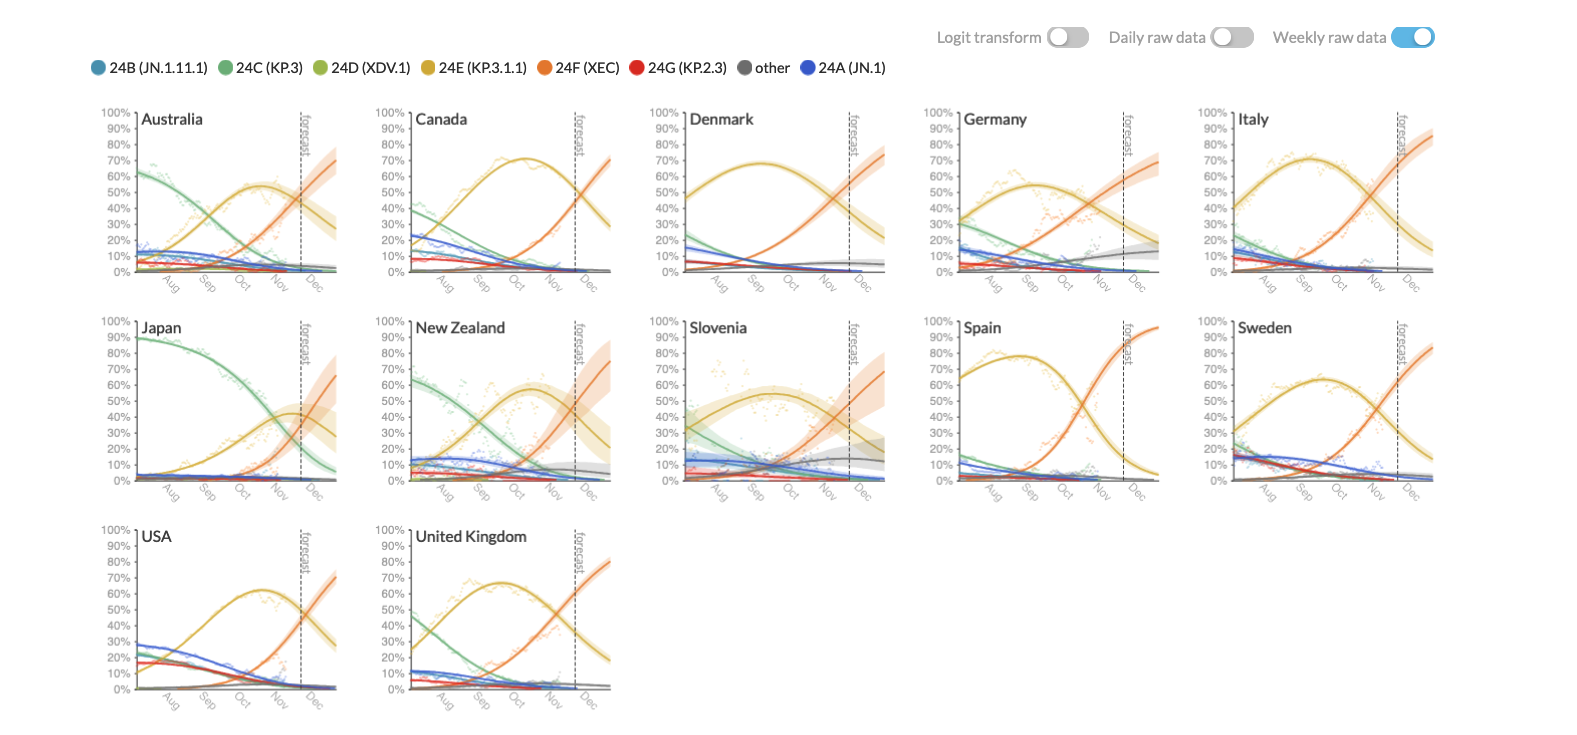
\includegraphics[width=1.0\linewidth]{./figures/clade_frequencies.png}
    \caption{
      \textbf{Live global SARS-CoV-2 frequency forecasts for Nextstrain clades.}
    }
    \label{fig:fn_clade_frequencies}
\end{figure}


\begin{figure}[h]
    \centering
    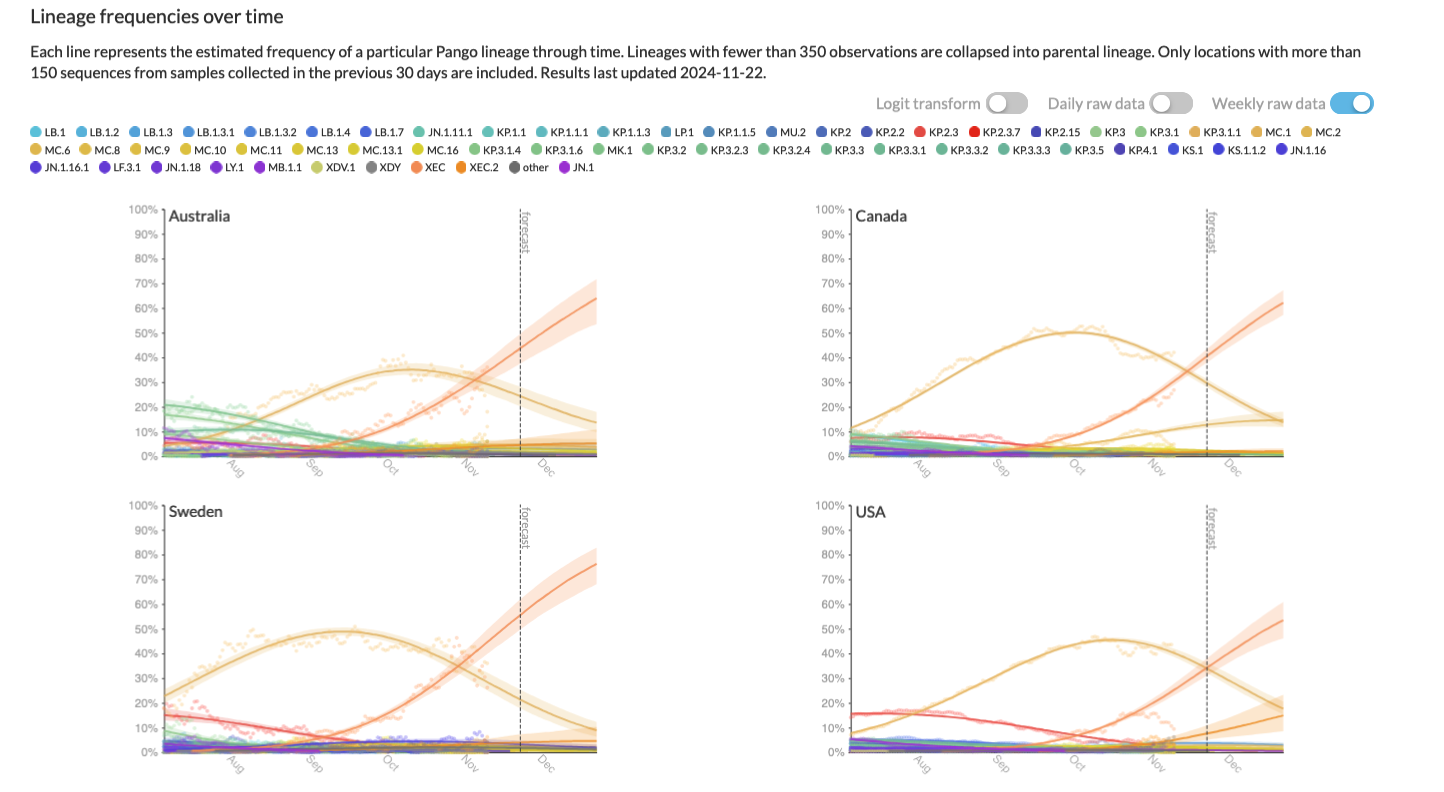
\includegraphics[width=1.0\linewidth]{./figures/lineage_frequencies.png}
    \caption{
      \textbf{Live global SARS-CoV-2 frequency forecasts for Pango lineages.}
    }
    \label{fig:fn_lineage_frequencies}
\end{figure}


\begin{figure}[h]
    \centering
    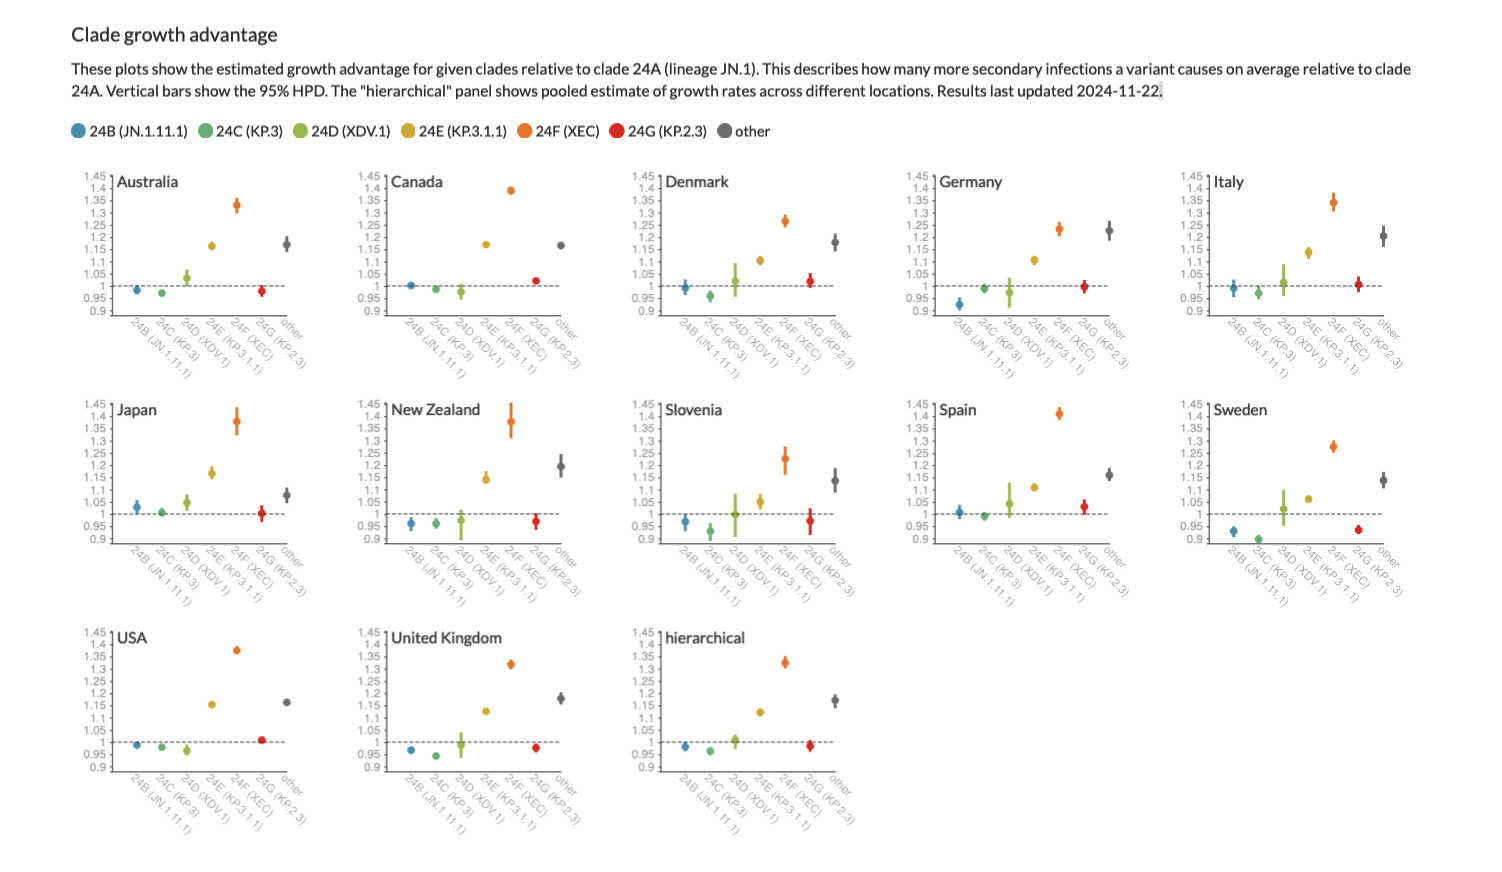
\includegraphics[width=1.0\linewidth]{./figures/clade_growth_advantages.png}
    \caption{
      \textbf{Live global SARS-CoV-2 growth advantage estimates for Nextstrain clades.}
    }
    \label{fig:fn_clade_growth_advantages}
\end{figure}


\begin{figure}[h]
    \centering
    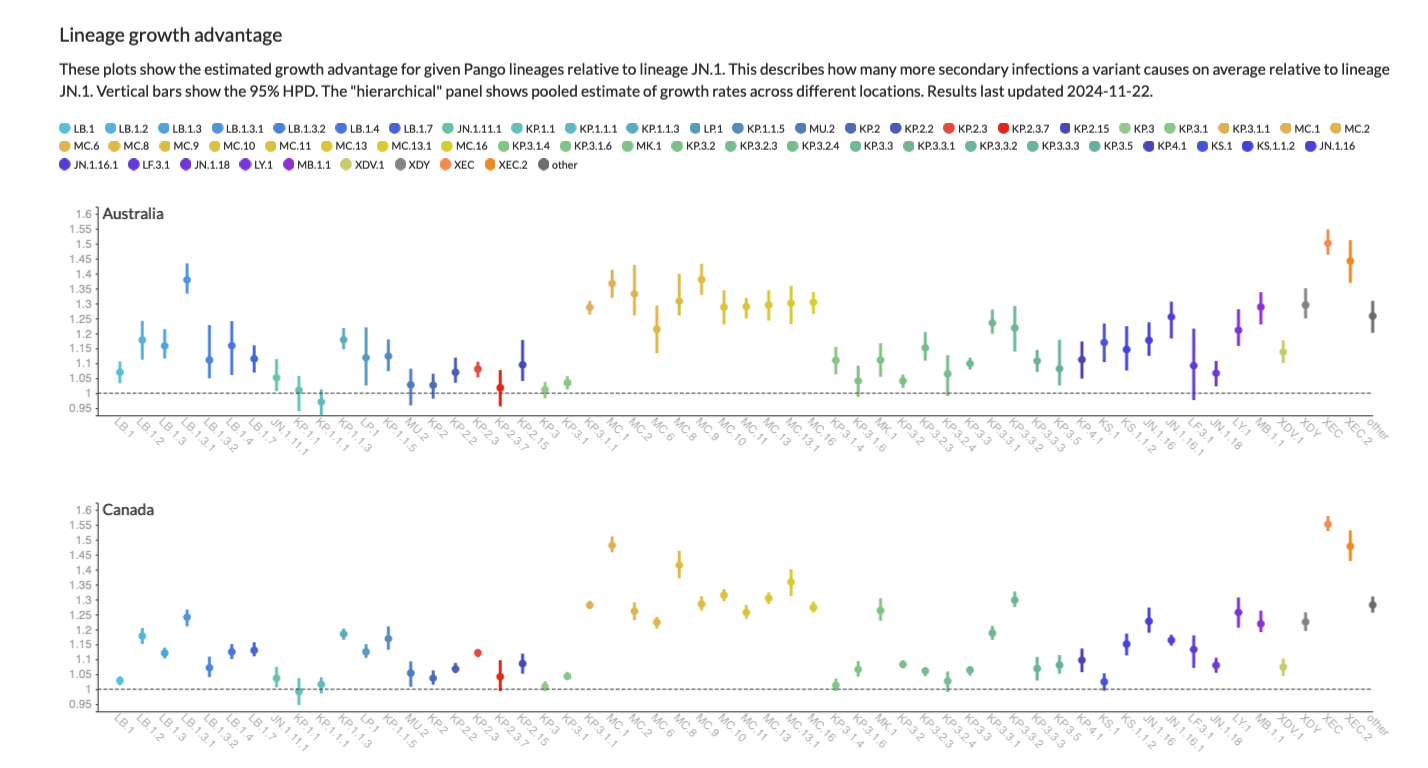
\includegraphics[width=1.0\linewidth]{./figures/lineage_growth_advantages.png}
    \caption{
      \textbf{Live global SARS-CoV-2 growth advantage estimates for Pango lineages.}
    }
    \label{fig:fn_lineage_growth_advantages}
\end{figure}


% ========== Chapter 7
\chapter{Conclusion}

% TODO: Frame the overarching challenge: understanding and forecasting SARS-CoV-2 variant dynamics by combining statistical models, mechanistic insights, and molecular data.

% TODO: Highlight the unifying principle of the thesis: mechanistic and biological structure, combined with statistical rigor, enhances forecast reliability and enables predictive power.

% TODO:Position the process of evaluation, mechanistic integration, and ... as the central driver of the thesis.

% TODO: Acknowledge remaining challenges, such as global inequities in data availability and limitations in predicting novel variants.

This dissertation establishes evolutionary forecasting as a rigorous and dynamic process by integrating insights from population genetics, mathematical epidemiology, and statistics. 
Through systematic evaluation, this work identifies gaps in existing models and lays a foundation for addressing them by integrating mechanistic insight with immunological, genetic, and epidemiological data.
Forecasting moves beyond tracking trends to become a dynamic process that unites real-time analysis, biological insight, and long-term evolutionary prediction. These advances rely on domain knowledge, statistical methodology, and data on the biological and environmental forces shaping pathogen evolution. They enable new kinds of predictions, such as variant-specific $R_t$, pseudo-immune representations, and epidemic growth rates derived from selective pressure, enhancing our ability to anticipate and respond to pathogen evolution.

This work presents several key contributions— mechanism-informed fitness models, forecasting evaluation methods, and data-informed fitness predictions— that deepen our understanding of pathogen evolution.
These contributions are operationalized through tools like \evofr\ and \forecastsNcov.
\evofr\ serves as a flexible toolkit for real-time analysis and forecasting while \forecastsNcov\ automates these methods to forecast in real-time, transforming methodological detail into accessible, reproducible insights for public health decision-makers.
Together, these contributions interpret today’s dynamics while predicting the evolution of tomorrow, turning theoretical advancements into modular, scalable systems capable of addressing diverse epidemiological and evolutionary challenges.

By emphasizing modularity and scalability, this work ensures its contributions extend beyond SARS-CoV-2 to other pathogens such as influenza or emerging zoonotic threats.
This adaptability, combined with interdisciplinary insights from genomics, immunology, epidemiology, computational biology, and statistics, strengthens our approach by ensuring it is both biologically meaningful and statistically robust.
These contributions provide the scientific and practical tools scientists and public health systems need to understand, interpret, and act on the dynamics of emerging genetic variants.

This dissertation advances evolutionary forecasting by integrating mechanistic insights and empirical data into models and tools that predict the dynamics of viral evolution. While significant progress has been made, the field presents opportunities for further development, particularly in capturing the complexity of viral evolution and ensuring the practical utility of forecasts.

A critical avenue for future research is expanding the scope of data incorporated into forecasting models. While this work demonstrates the power of genomic surveillance, viral evolution is influenced by behavioral, clinical, and environmental factors that are not yet fully integrated.
Incorporating these dimensions would enhance the fitness-based models developed here, offering a richer understanding of the factors shaping variant success and public health outcomes.

The methodologies presented in this dissertation, though tailored to SARS-CoV-2, suggest broader applicability to other rapidly evolving pathogens such as influenza and RSV.
Generalizing these models will require adapting them to the specific evolutionary and immunological dynamics of other viruses.
This extension would establish evolutionary forecasting as a universal framework for monitoring and predicting pathogen evolution.

At the same time, developing generative sequence models offers a promising direction.
Such models could simulate evolutionary trajectories, predicting not only which variants may emerge but also their phenotypic traits while basing generation in our mechanistic understanding of pathogen evolution.
These capabilities would build on the fitness and immune escape dynamics studied here, enabling long-term forecasting and preemptive public health strategies.

Further refinement of population structure in these models is also essential.
Selective pressures and fitness vary across populations due to differences in immunity, geography, and temporal dynamics.
Building on the latent factor models developed in this dissertation, future work can better account for these variations, improving the precision of forecasts across diverse contexts.

On a practical level, this dissertation demonstrates how tools like \evofr\ and \forecastsNcov\ can operationalize evolutionary forecasting.
To maximize their impact, future efforts should focus on making these tools more accessible to public health practitioners through user-friendly interfaces and seamless integration into existing workflows.
Collaboration between evolutionary biologists, immunologists, virologists, and public health experts will be critical for validating these models and ensuring their relevance in real-world decision-making.

Finally, as forecasting tools become increasingly influential in guiding vaccine updates and public health policies, their practical and policy consequences require careful consideration.
Future work should explore frameworks to ensure forecasts are used transparently and equitably, addressing issues such as resource allocation and public communication.

The next phase of evolutionary forecasting lies in refining its scientific foundations while expanding its practical applications.
By integrating diverse data sources, adapting models to new pathogens, and addressing the practical impact of these forecasts, the field can continue to evolve, meeting the needs of both science and society.

%TODO: Mention specifically longitudinal immune profiling data and that the reality is that data availability is declining and we need methods that can make due with what we have and suggest cost-effective means of expanding data collection

In my opinion, this work offers a clear lesson beyond advancing forecasting or any single pathogen.
It has shown that pursuing a deeper understanding of dynamic systems and the structures that drive them creates new opportunities for innovation.
In that understanding lies the potential to anticipate, to prepare, and to act.


\printendnotes

%
% ==========   Bibliography
%
% \nocite{*}   % include everything in the uwthesis.bib file
\bibliographystyle{plain}
\bibliography{dissertation_Figgins}
%
% ==========   Appendices
%
\appendix
\raggedbottom\sloppy

\graphicspath{{./chapters/rt-from-frequency-dynamics/}}
\chapter{Supplementary Materials for Chapter 2} 

%TODO: Make sure we use supplementary results -> supplementary figures

\section{Supplementary Text}

\subsection*{Relationship to multinomial logistic regression}

Other papers have tried to infer growth advantages of variants from sequence data alone, we show that the multinomial logistic regression model typically used in these analysis is roughly equivalent to our fixed growth advantage model, but that inferring relative effective reproduction numbers between variants using multinomial logistic regression requires additional restrictions on the generation time.
Multinomial logistic regression typically models the probability of a given observation belong to class $v$ at time $t$ as
\begin{equation}
  f_{v}(t) = \frac{p_{v}\exp(\beta_{v} t)}{\sum_{1\leq u\leq V} p_{u}\exp(\beta_{u} t)}.
\end{equation}
For our purpose, we can assume this probability is equivalent to the true frequency of variant $v$ in the population and in this case, $p_{v}$ is considered to be related to the prevalence on variant $v$ in the population at $t=0$ and $\beta_{v}$ can be considered to be the growth advantage relative to a pivot class $u_{*}$ which has $\beta_{k_{*}} = 0$.
In order to see the connection between the above model and ours, we return to the original renewal equation of the form
\begin{equation}
  I(t) = R_{t}\int_{0}^{t} I(t-\tau) g(\tau).
\end{equation}
Assuming that $g$  is a point mass at a mean generation time $T_{g}$, we have that
\begin{equation}
  I(nT_{g}) = \left(\prod_{i=1}^{n} R_{iT_{g}}\right) I(0).
\end{equation}
Assuming that there are several variants following these same dynamics, we have that the frequency of a given variant $v$ can be written as
\begin{equation}
  f_{v}(nT_{g}) = \frac{I_{v}(nT_{g})}{\sum_{1\leq u \leq V} I_{u}(nT_{g})}.
\end{equation}
If we assume a constant growth advantage as in our model, we then have that $R_{t,v} = \Delta_{v} R_{t}$, so that
\begin{equation}
  f_{v}(nT_{g}) =  \frac{\Delta_{v}^{n} I_{v}(0)}{\sum_{1\leq u \leq V} \Delta_{u}^{n} I_{u}(0)}.
\end{equation}
Writing $\Delta_{v} = \exp(\delta_{v})$ and $t = n T_{g}$, allows us to see that
\begin{equation}
  f_{v}(t) = \frac{I_{v}(0) \exp(\frac{\delta_{v}}{T_{g}} t)}{\sum_{1\leq u \leq V}I_{u}(0) \exp(\frac{\delta_{u}}{T_{g}} t)}.
\end{equation}
By fixing one pivot class so that $I_{u_{*}} = 1$ and $\delta_{u_{*}} / T_{g} = 0$, we can identify our model with the multinomial logistic regression by relating the parameters as

\begin{align}
  \delta_{v} &= \beta_{v}T_{g}\\
  I_{v}(0) &= p_{v}.
\end{align}

This shows that the multinomial logistic regression functions similarly to our fixed growth advantage model except with the additional assumption that the generation time is a point mass at $T_{g}$.
This assumption additionally allows us to relate the epidemic growth rate $r$ and the effective reproduction number as $R = \exp(r T_{g})$ \cite{Wallinga2006}.
Therefore, by further assuming that the variant infections are exponentially growing with rates $r_{v}$, we can then identify $\beta_{v} = r_{v} - r_{u_{*}}$.
This means that the relative effective reproduction number for any two variants can be written as
\begin{align*}
\ln \left( \frac{R_{t,v}}{R_{t,u}} \right) = (\beta_{v} - \beta_{u}) T_{g}.
\end{align*}

\begin{figure}
  \centering
  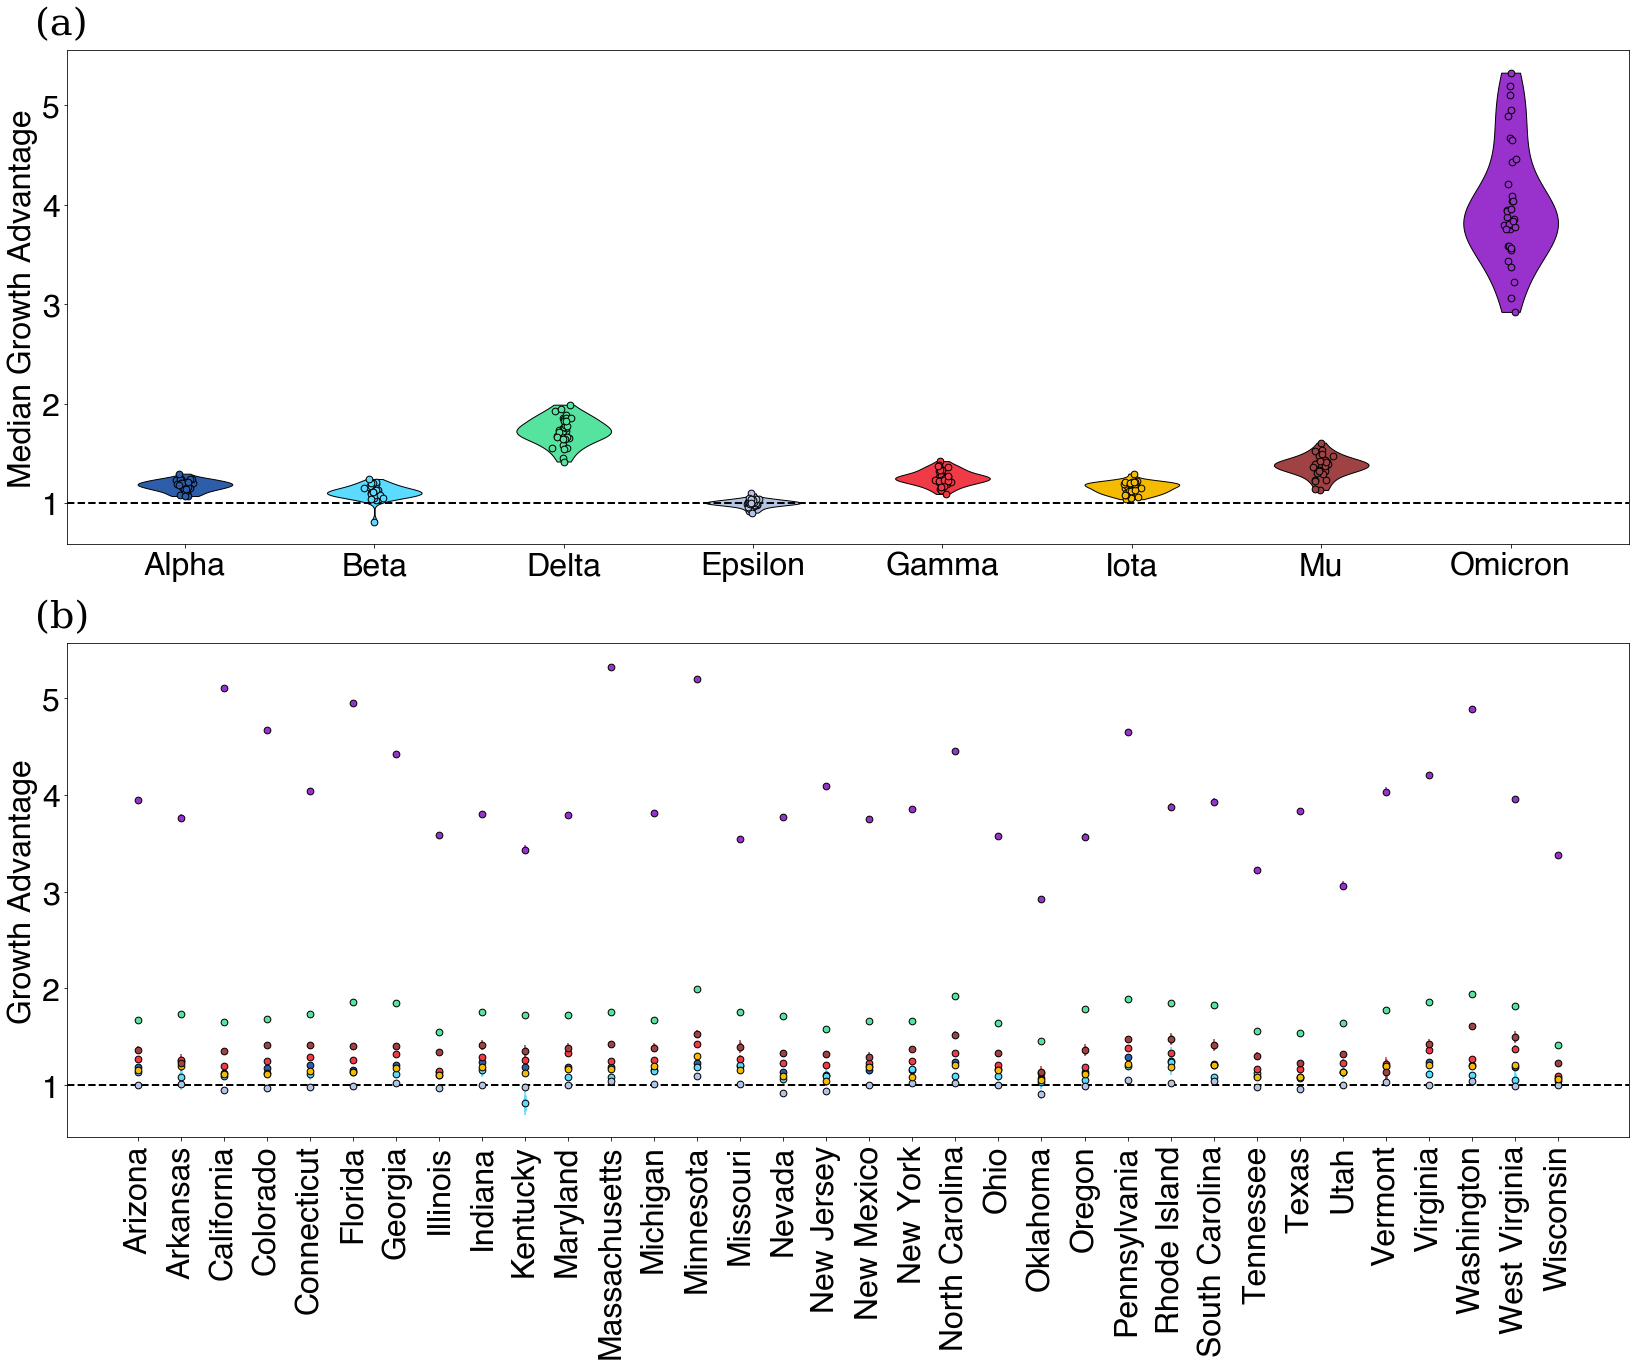
\includegraphics[width=\linewidth]{figs/fig_MLR_growth_advantages_supp.png}
  \caption{Estimating variant growth advantages in various states using Multinomial Logistic Regression model assuming generation time $T_{g} = 5.2$.
  (a) Growth advantages visualized by state.
  (b) Same as (a) but grouped by variant.}%
  \label{fig:MLR_growth_advantages}
\end{figure}

\newpage

\subsection*{Relating epidemic growth rates to relative effective reproduction numbers}

An important relationship of interest is between the epidemic growth rate of an epidemic and its effective reproduction number.
In the case of our analysis, we are particularly interested in the effect of generation time assumptions on estimated variant-specific effective reproduction numbers.
First, notice that the effective reproduction number and the epidemic growth rate of an epidemic are related by
\begin{align*}
R_{t} = \frac{1}{\int_{0}^{\infty} \exp(-r\tau)g(\tau)d\tau} = \frac{1}{M_{g}(-r)}
\end{align*}
according to the Lotka-Euler equation \cite{Wallinga2006} where $r$ is the epidemic growth rate and $M_{g}$ is the moment-generating function of the generation time $g$.

This allows us to write the relative reproduction number of two variants $v$ and $u$ as a function of their epidemic growth rates, so that
\begin{align*}
\frac{R_{t,v}}{R_{t,u}} = \frac{M_{g}(-r_{u})}{M_{g}(-r_{v})}.
\end{align*}

We'll consider three common generation time assumptions. First, we consider the case where the generation time is a point mass at $T_{g}$. In which case, $M_{g}(-r) = \exp(-r T_{g})$ and we recover the relationship
\begin{align*}
R_{t,v} = \exp(r_{v}T_{g}).
\end{align*}

In this case, the relative effective reproduction number will depend on only the difference between the epidemic growth rates and therefore, is commonly used when converting estimated growth advantages to relative reproduction numbers in the case of logistic growth models.

Second, we consider the case where the generation time is an exponential distribution with mean $T_{g}$. This assumption is often implicit and common in models of infectious diseases such as ODEs and their stochastic variants. Using the corresponding moment-generating function, we see that
\begin{align*}
R_{t,v} = 1 + r_{v} T_{g}
\end{align*}

Next, we consider the Gamma distributed generation times with mean $T_{g}$ and standard deviation $s$.
This is often used in models of infectious diseases via the chain trick in which multiple compartments are chained together to obtain non-exponential generation times or infectious periods.
Re-parameterizing the Gamma distribution in terms of its mean and standard deviation and using its moment generating function, we have that
\begin{align*}
R_{t,v} = \left(1 + r_{v}  \left(\frac{s^{2}}{T_{g}}\right) \right)^{T_{g}^{2} / s^{2}}.
\end{align*}

From this equation, we can see that increases in the mean of the generation time of $v$ leads to decreasing estimates of $R_{t,v}$ during epidemic decline ($r_{v} < 0$) and increased estimates during epidemic growth ($r_{v} > 0$) assuming $r_{v}$ and $s$ are fixed.
Additionally, increases in the standard deviation will generally lead to lower inferred variant advantages.
This effect is also visualized in Figure \ref{fig:generation_time_sensitivity}.

\paragraph{Variant growth-advantages are sensitive to generation time}%

In the case where we have two variants $u, v$ with Gamma-distributed generation times with means $T_{u}, T_{v}$ and standard deviations $s_{u}, s_{v}$ respectively, we can then write the relative effective reproduction number of $v$ over $u$ as
\begin{align*}
\frac{R_{t,v}}{R_{t,u}} = \frac{\left[1 + r_{v}  \left(\frac{s_{v}^{2}}{T_{v}}\right)\right]^{T_{v}^{2} / s_{v}^{2}}}{\left[1 + r_{u} \left(\frac{s_{u}^{2}}{T_{u}}\right)\right]^{T_{u}^{2} / s_{u}^{2}}}.
\end{align*}
It follows that increases in the mean of the generation time of $v$ leads to decreasing inferred variant advantages during epidemic decline and increased advantages during epidemic growth when all quantities are fixed.
On the other hand, increases in the standard deviation will generally lead to lower inferred variant advantages.

Taking a logarithm, we can also evaluate the sensitivity of our inferred growth advantages from our fixed growth advantage model with respect to the generation time assuming it is Gamma distributed as
\begin{align*}
 \delta_{v}  = \ln \left( \frac{R_{t,v}}{R_{t,0}} \right) = \left( \frac{T_{g}^{2}}{s^{2}} \right)  \ln \left( \frac{1 + r_{v}  \left(\frac{s^{2}}{T_{g}}\right)}{1 + r_{0} \left(\frac{s^{2}}{T_{g}}\right) } \right).
\end{align*}
As the log of the relative effective reproduction number, the behavior here is analogous to that discussed above when the mean $T_{g}$ and standard deviation $s$ are changed.
This effects of varying mean and standard deviation are illustrated in Figure \ref{fig:growth_advantage_sensitivity}.
Although the effective reproduction number and the growth advantage appear to have strong dependence on generation time parameters, we find that the epidemic growth rate $r$ is more robust to changes in generation time (see Figure \ref{fig:little_r_sensitivity}).

The cases of exponential and Gamma-distributed generation times highlight that for non-deterministic generation times there is no guarantee that the relative effective reproduction number depends on only the difference in epidemic growth rates.
In fact, these estimates based on the deterministic generation times correspond to the case in which the standard deviation shrinks zero, they are likely overestimates of variant advantages given the observed variation in the serial interval of SARS-CoV-2 infections.

\paragraph{Fixed growth advantages become time-varying under generation time misspecification}

We'll now consider the case where there is a true fixed-variant growth advantage. Suppose for a two-variant system that $\delta$ is the constant (log) growth advantage of the variant virus over the wildtype under the variant generation time $g_{T}$, so that $\delta = \ln \left( R_{t,v}^{g_{T}} / R_{t, wt}^{g_{T}} \right)$.
Here subscripts denote the generation time used when computing $R_{t}$.

Under the misspecified variant generation time $g_{M}$, we can then write the inferred growth advantage as
\begin{align*}
  \delta_{M} &= \ln \left( \frac{R_{t,v}^{g_{M}}}{R_{t, wt}^{g_{T}}} \right) = \ln \left(\frac{R_{t,v}^{g_{M}}}{R_{t,v}^{g_{T}}}\right) + \delta.
\end{align*}

In general, the term inside the log is non-constant meaning that fixed variant growth advantages under one generation time become non-constant under generation time specification.

\begin{figure}
  \centering
  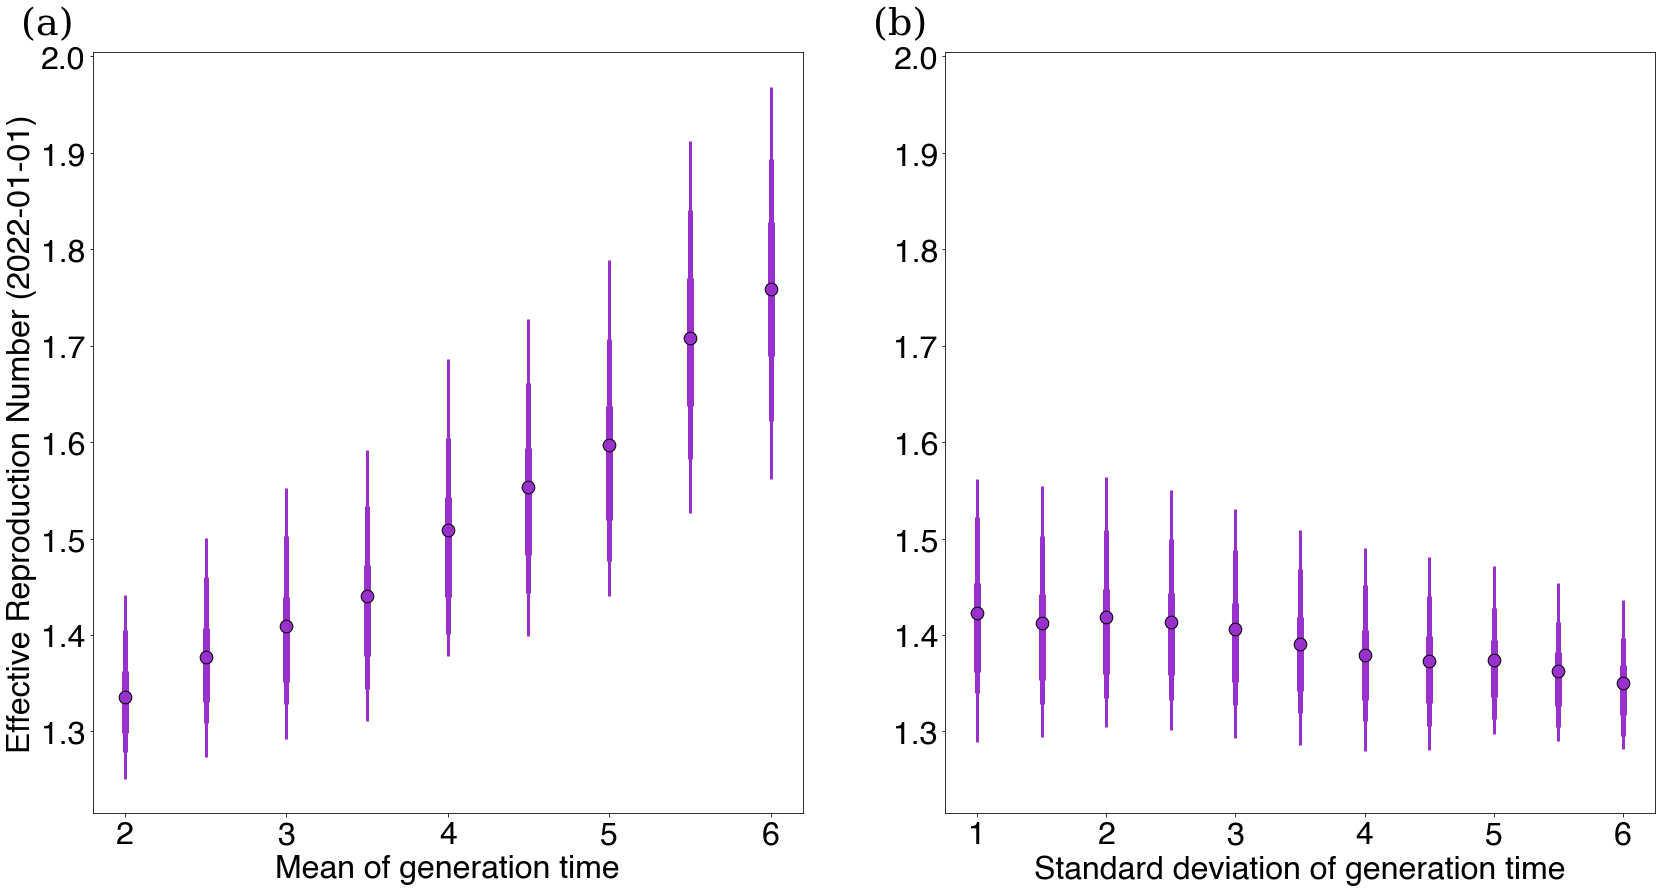
\includegraphics[width=\linewidth]{figs/generation_time_sensitivity.png}
  \caption{\textbf{Sensitivity of effective reproduction number to changes in generation time.}
(a) We vary the mean of Omicron generation time keeping a constant standard deviation 1.2 and plot against effective reproduction number estimates for Omicron in Washington state on February 1st, 2022 using our GARW model.
(b) The same as (a), but we instead vary the standard deviation of Omicron generation time keeping a constant mean 3.1.}%
  \label{fig:generation_time_sensitivity}
\end{figure}

\begin{figure}
  \centering
  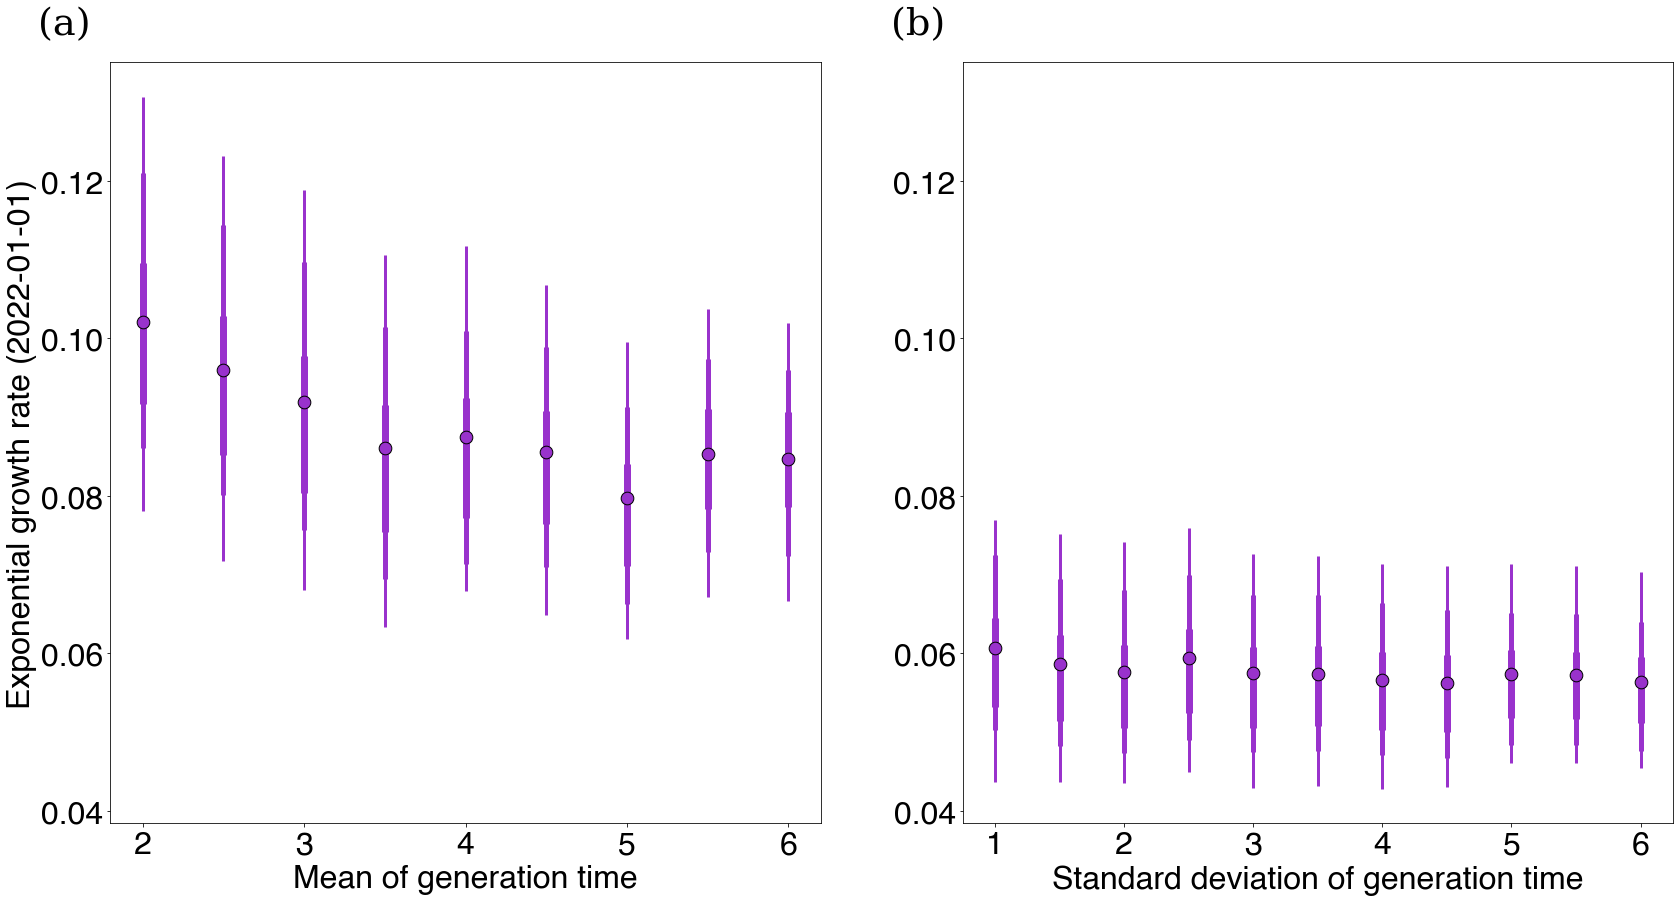
\includegraphics[width=\linewidth]{figs/little_r_sensitivity.png}
  \caption{\textbf{Sensitivity of epidemic growth rates to changes in generation time.}
(a) We vary the mean of Omicron generation time keeping a constant standard deviation 1.2 and plot against exponential growth rates for Omicron in Washington state on February 1st, 2022 using our GARW model and assuming a Gamma-distributed generation time.
(b) The same as (a), but we instead vary the standard deviation of Omicron generation time keeping a constant mean 3.1. }%
  \label{fig:little_r_sensitivity}
\end{figure}

\begin{figure}
  \centering
  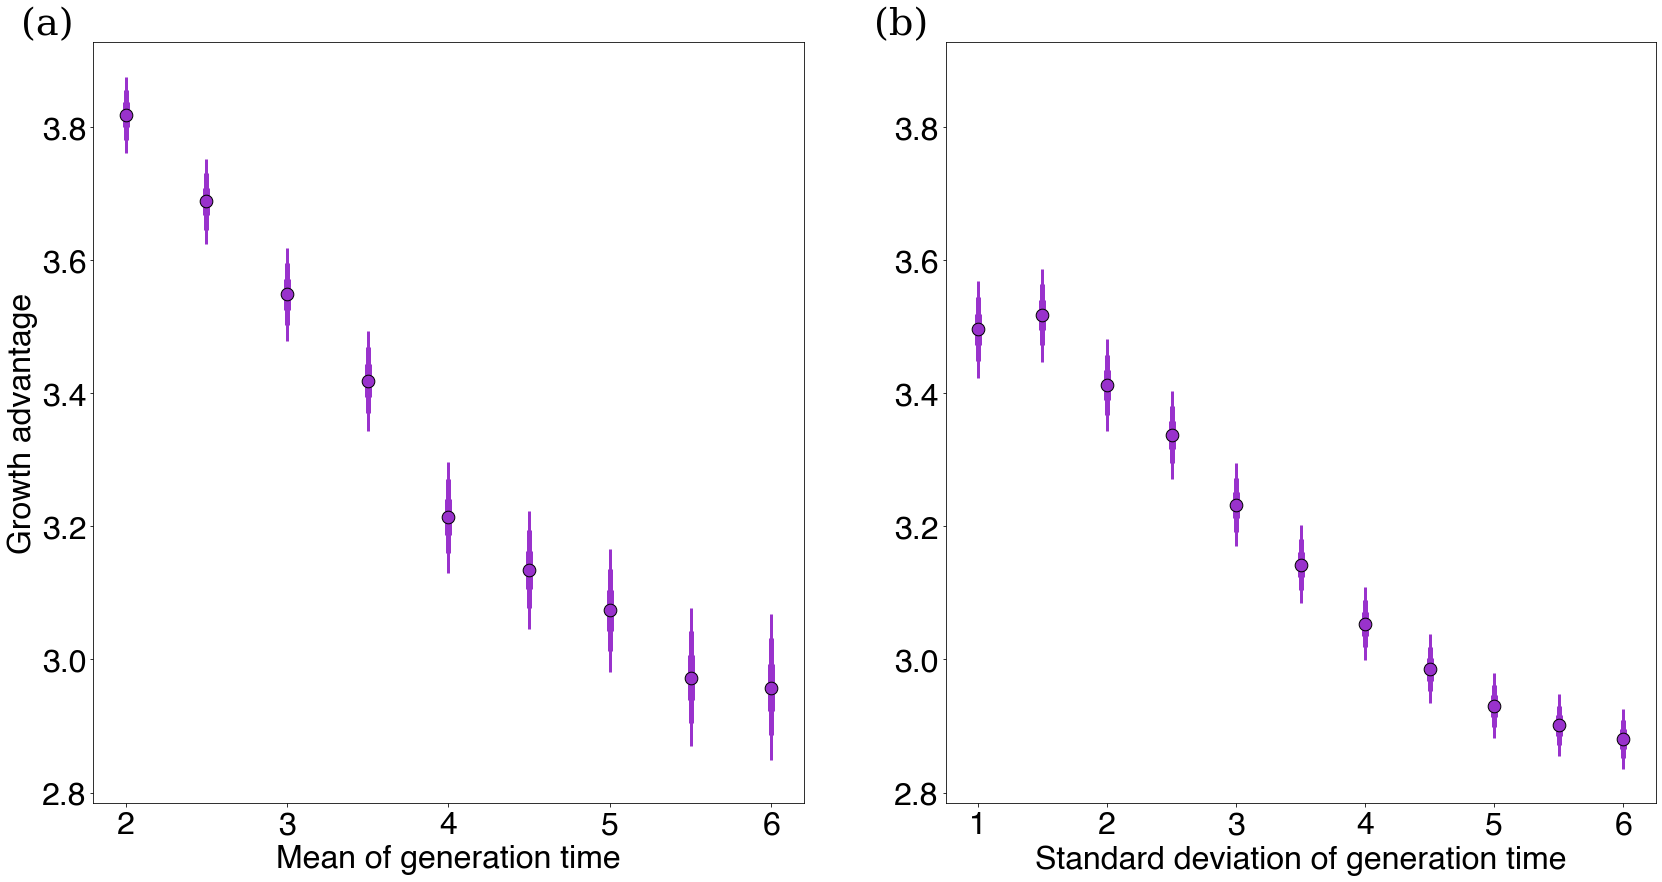
\includegraphics[width=\linewidth]{figs/growth_advantage_sensitivity.png}
  \caption{\textbf{Sensitivity of growth advantages to changes in generation time.}
(a) We vary the mean of Omicron generation time keeping a constant standard deviation 1.2 and plot against exponential growth rates for Delta in Washington state on July 1st, 2021 using our fixed growth model.
(b) The same as (a), but we instead vary the standard deviation of Omicron generation time keeping a constant mean 3.2.}%
  \label{fig:growth_advantage_sensitivity}
\end{figure}

\section{Supplementary Figures}

\begin{figure}
  \centering
  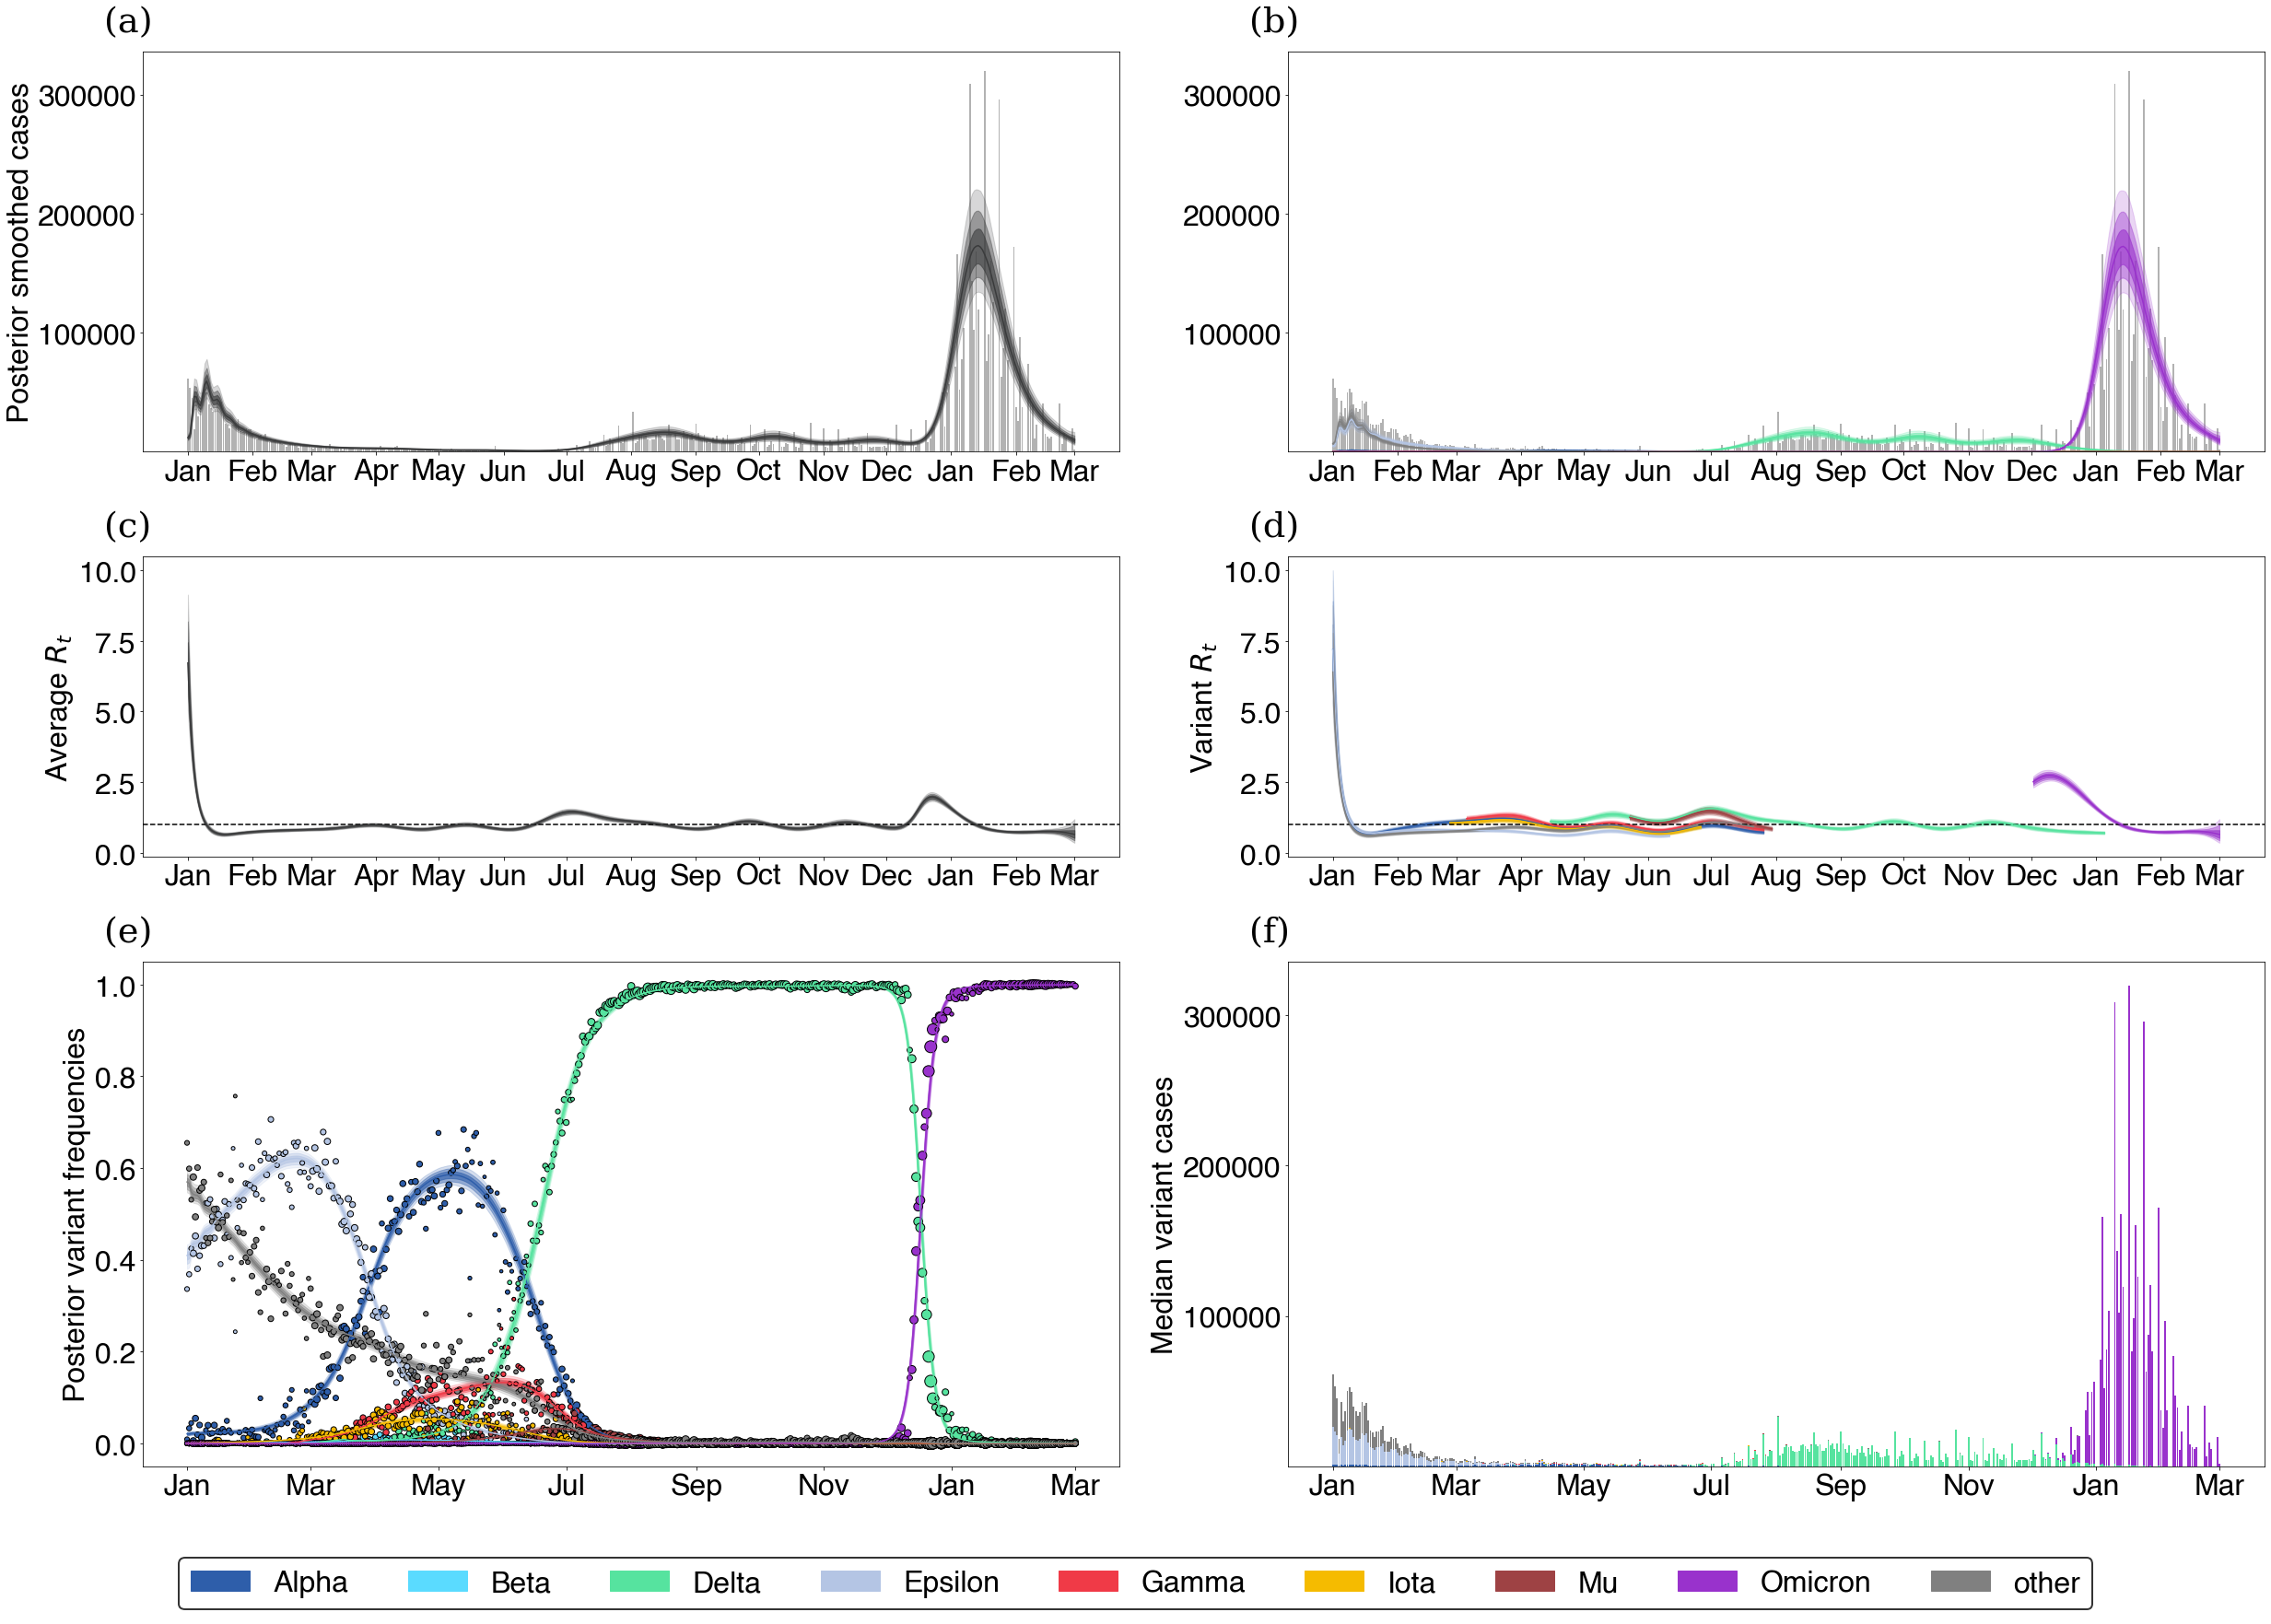
\includegraphics[width=\linewidth]{figs/GARW_rt_California.png}
  \caption{\textbf{Fitting the GARW model to California data.}}%
  \label{fig:GARW_rt_California}
\end{figure}

\begin{figure}
  \centering
  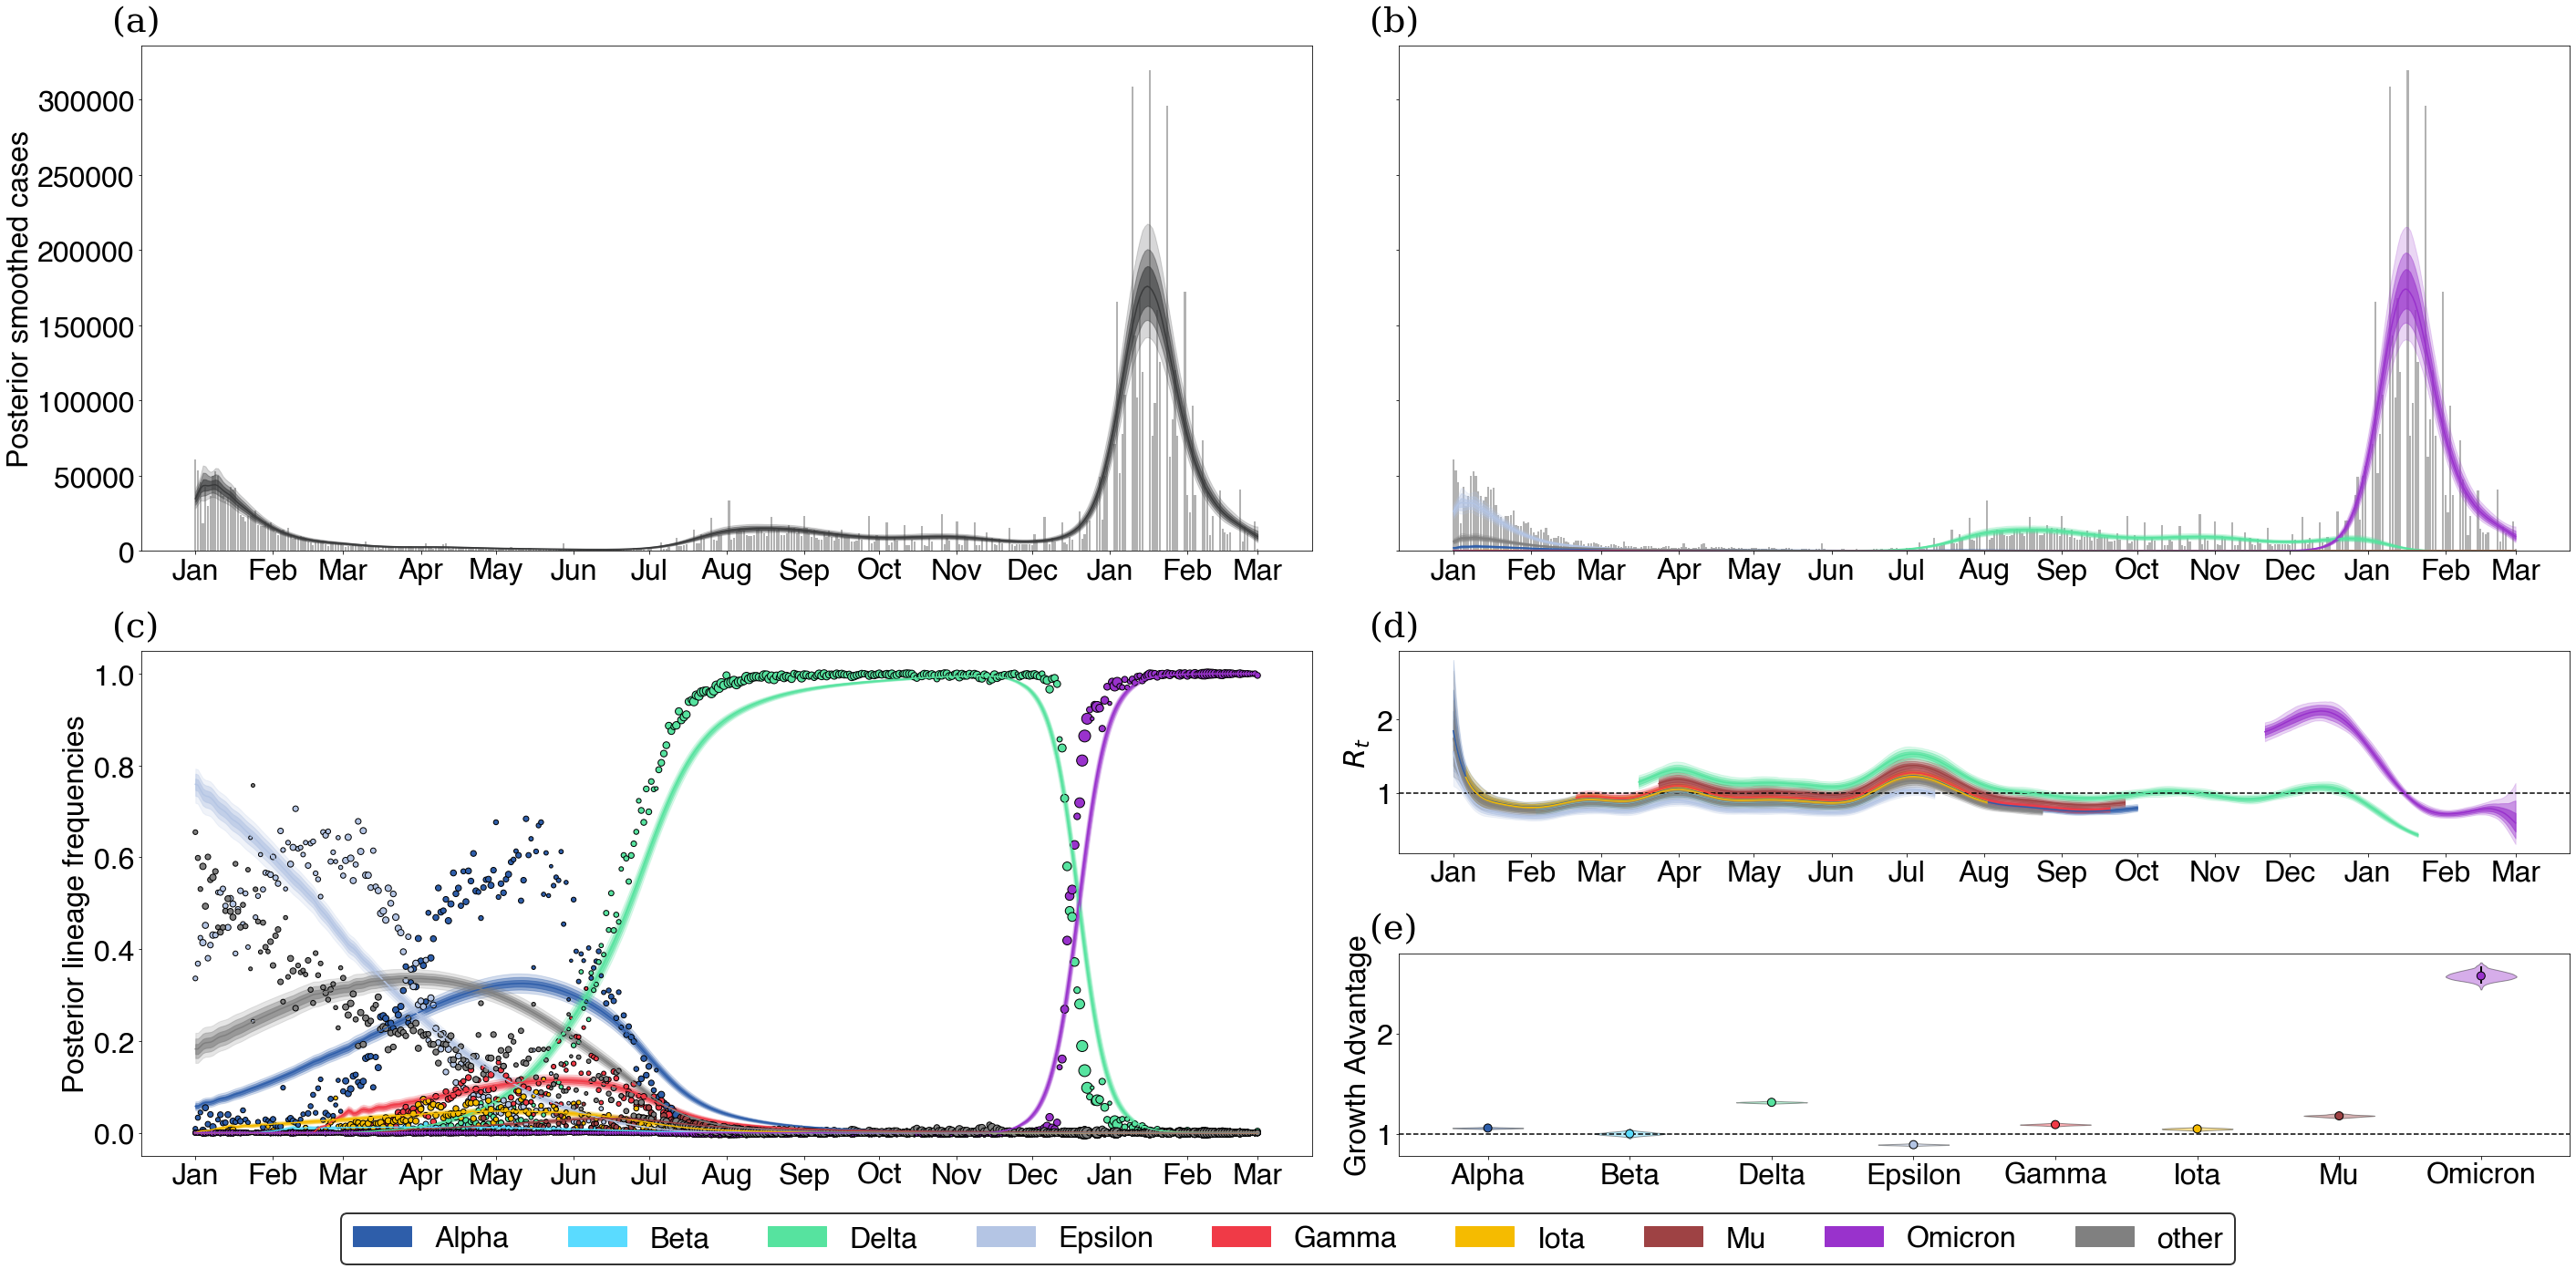
\includegraphics[width=\linewidth]{figs/fixed_growth_California.png}
  \caption{\textbf{Fitting the fixed growth advantage model to California data.}}%
  \label{fig:fixed_growth_California}
\end{figure}

\begin{figure}
  \centering
  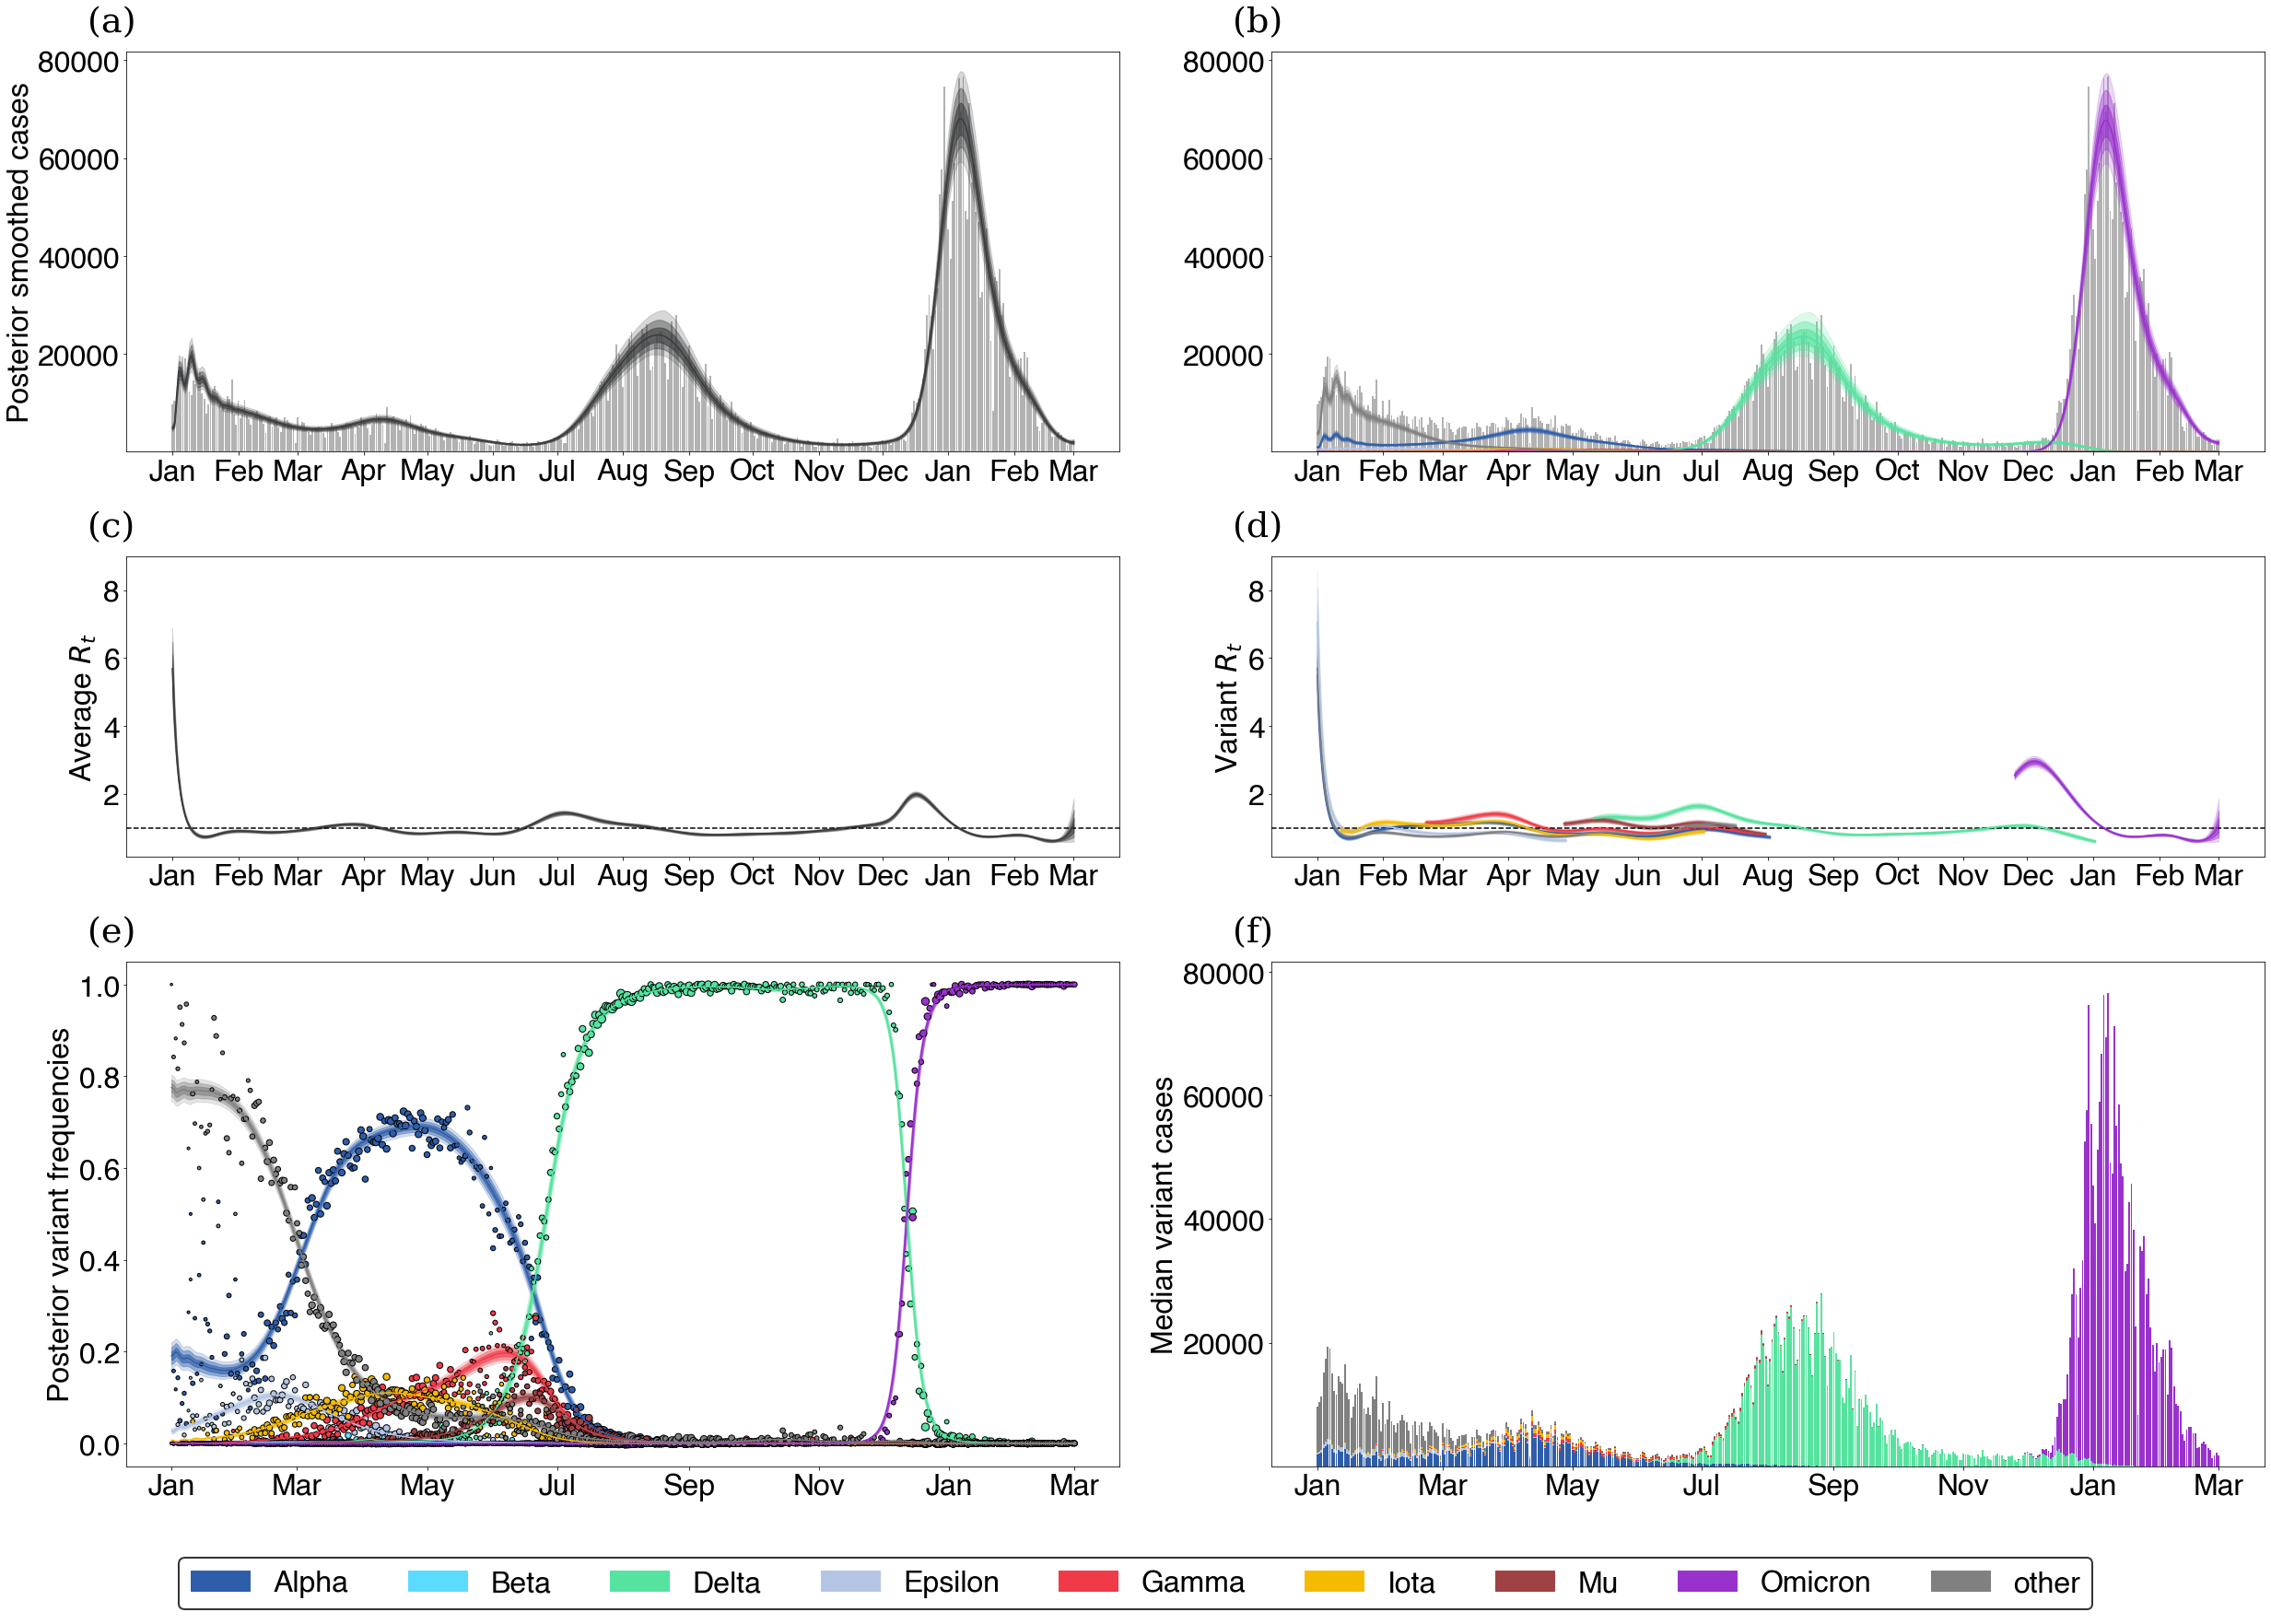
\includegraphics[width=\linewidth]{figs/GARW_rt_Florida.png}
  \caption{\textbf{Fitting the GARW model to Florida data.}}%
  \label{fig:GARW_rt_Florida}
\end{figure}

\begin{figure}
  \centering
  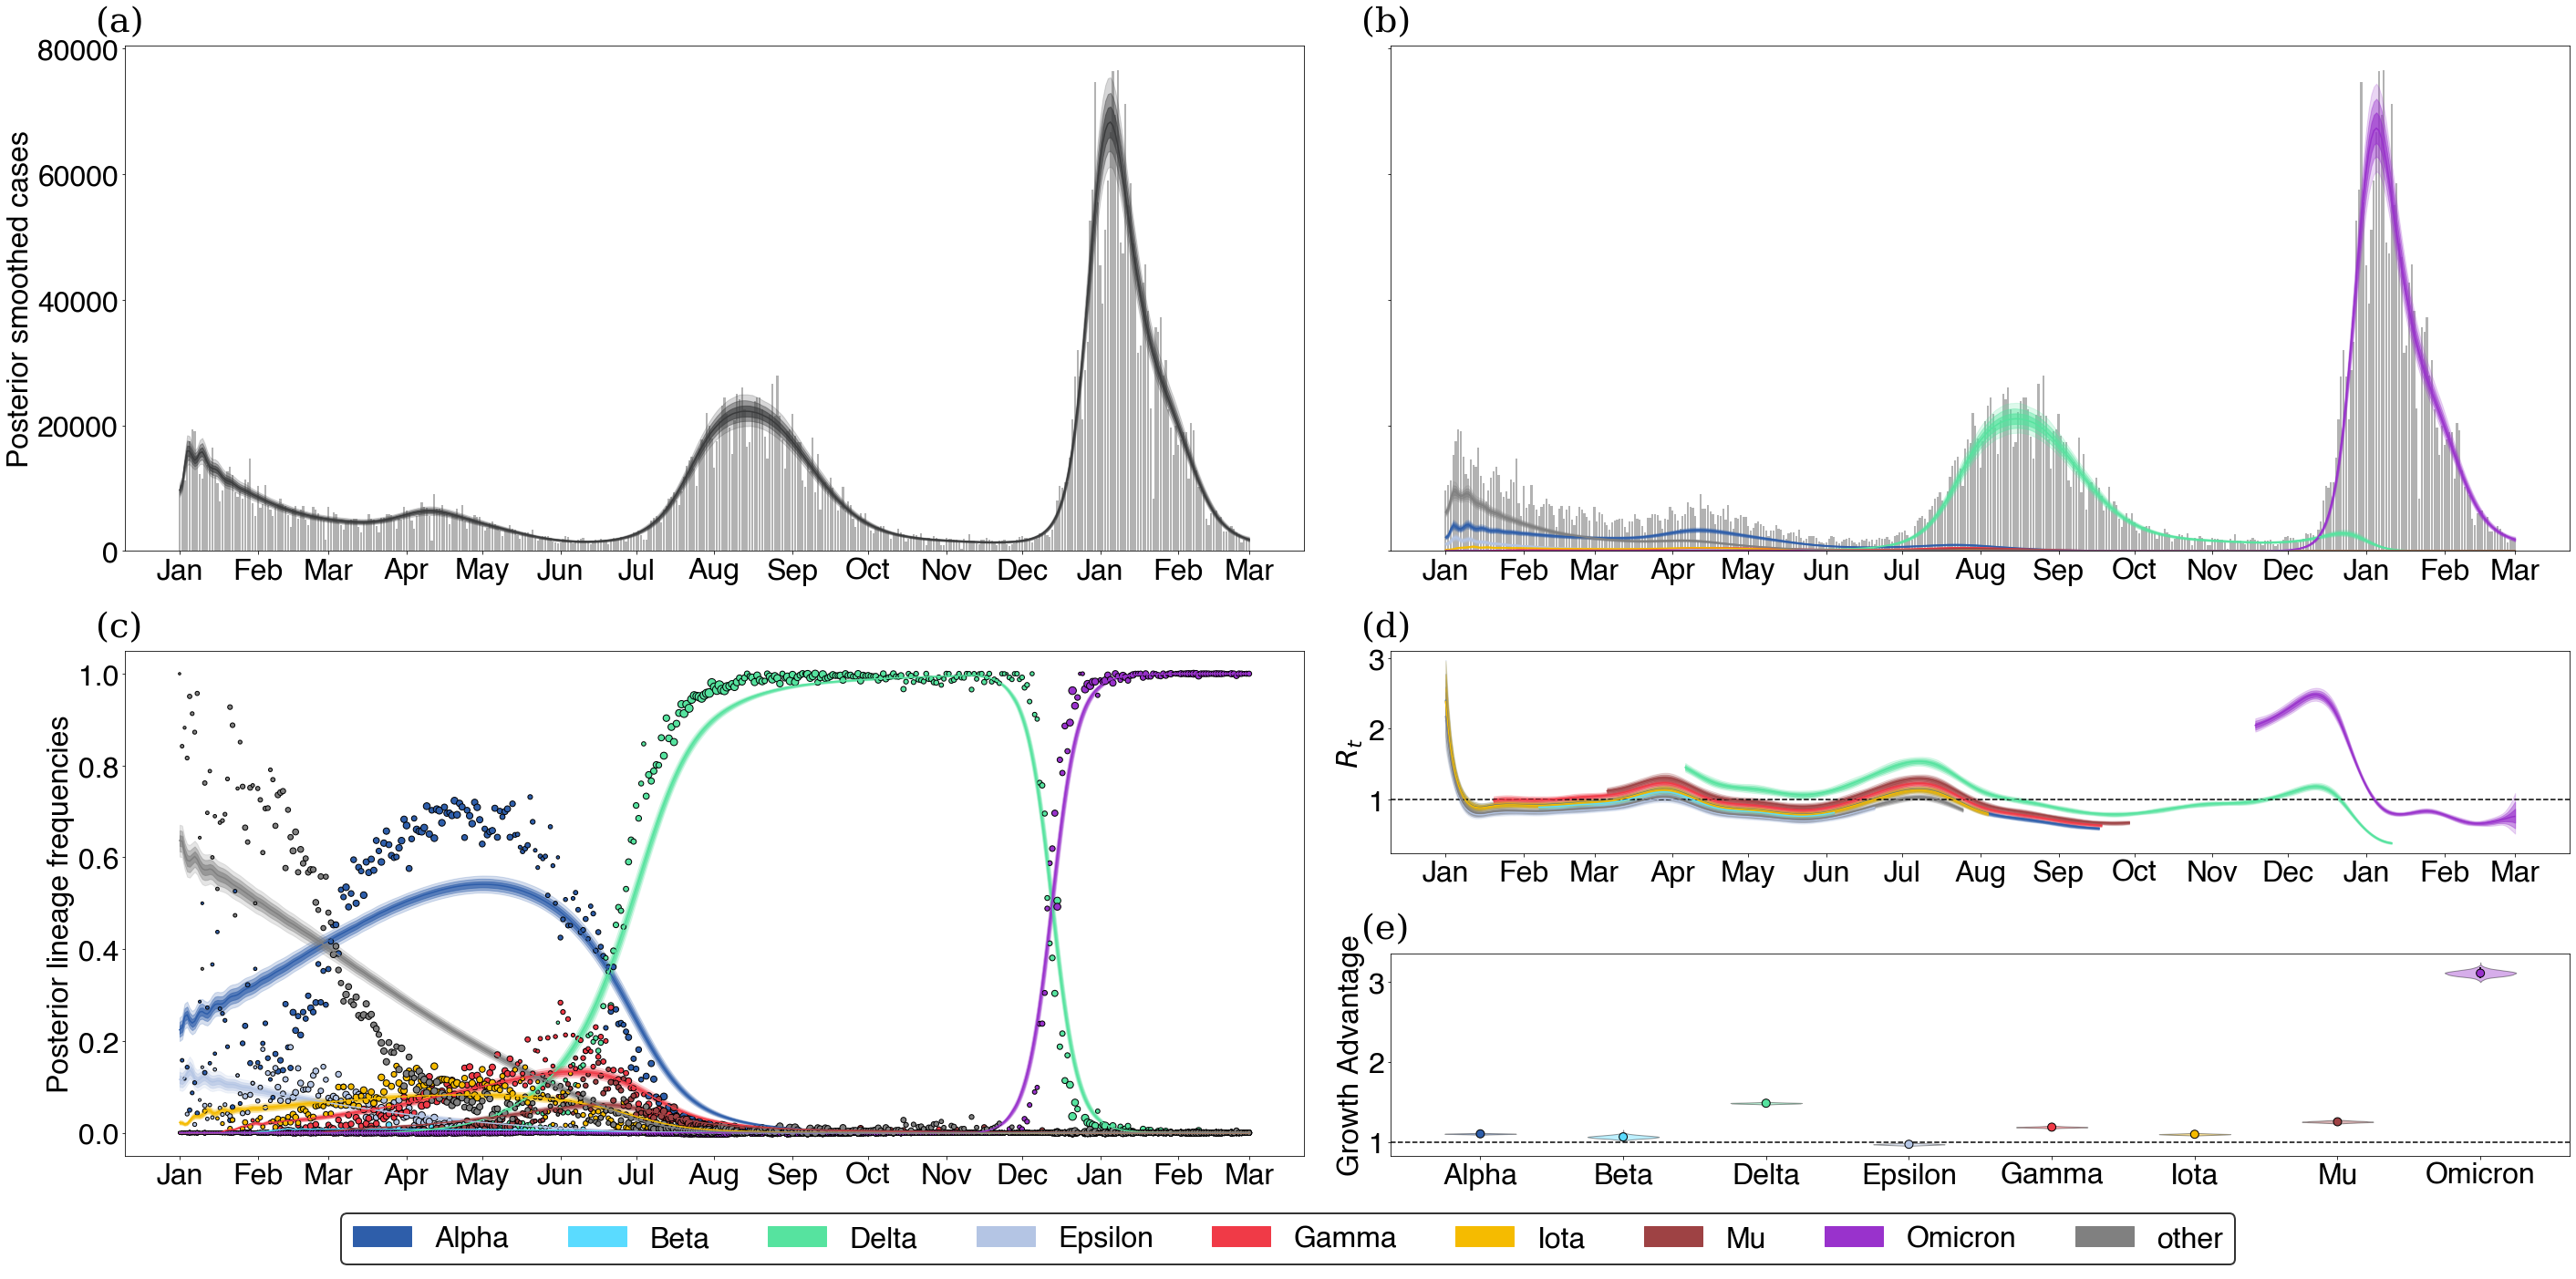
\includegraphics[width=\linewidth]{figs/fixed_growth_Florida.png}
  \caption{\textbf{Fitting the fixed growth advantage model to Florida data.}}%
  \label{fig:fixed_growth_Florida}
\end{figure}

\begin{figure}
  \centering
  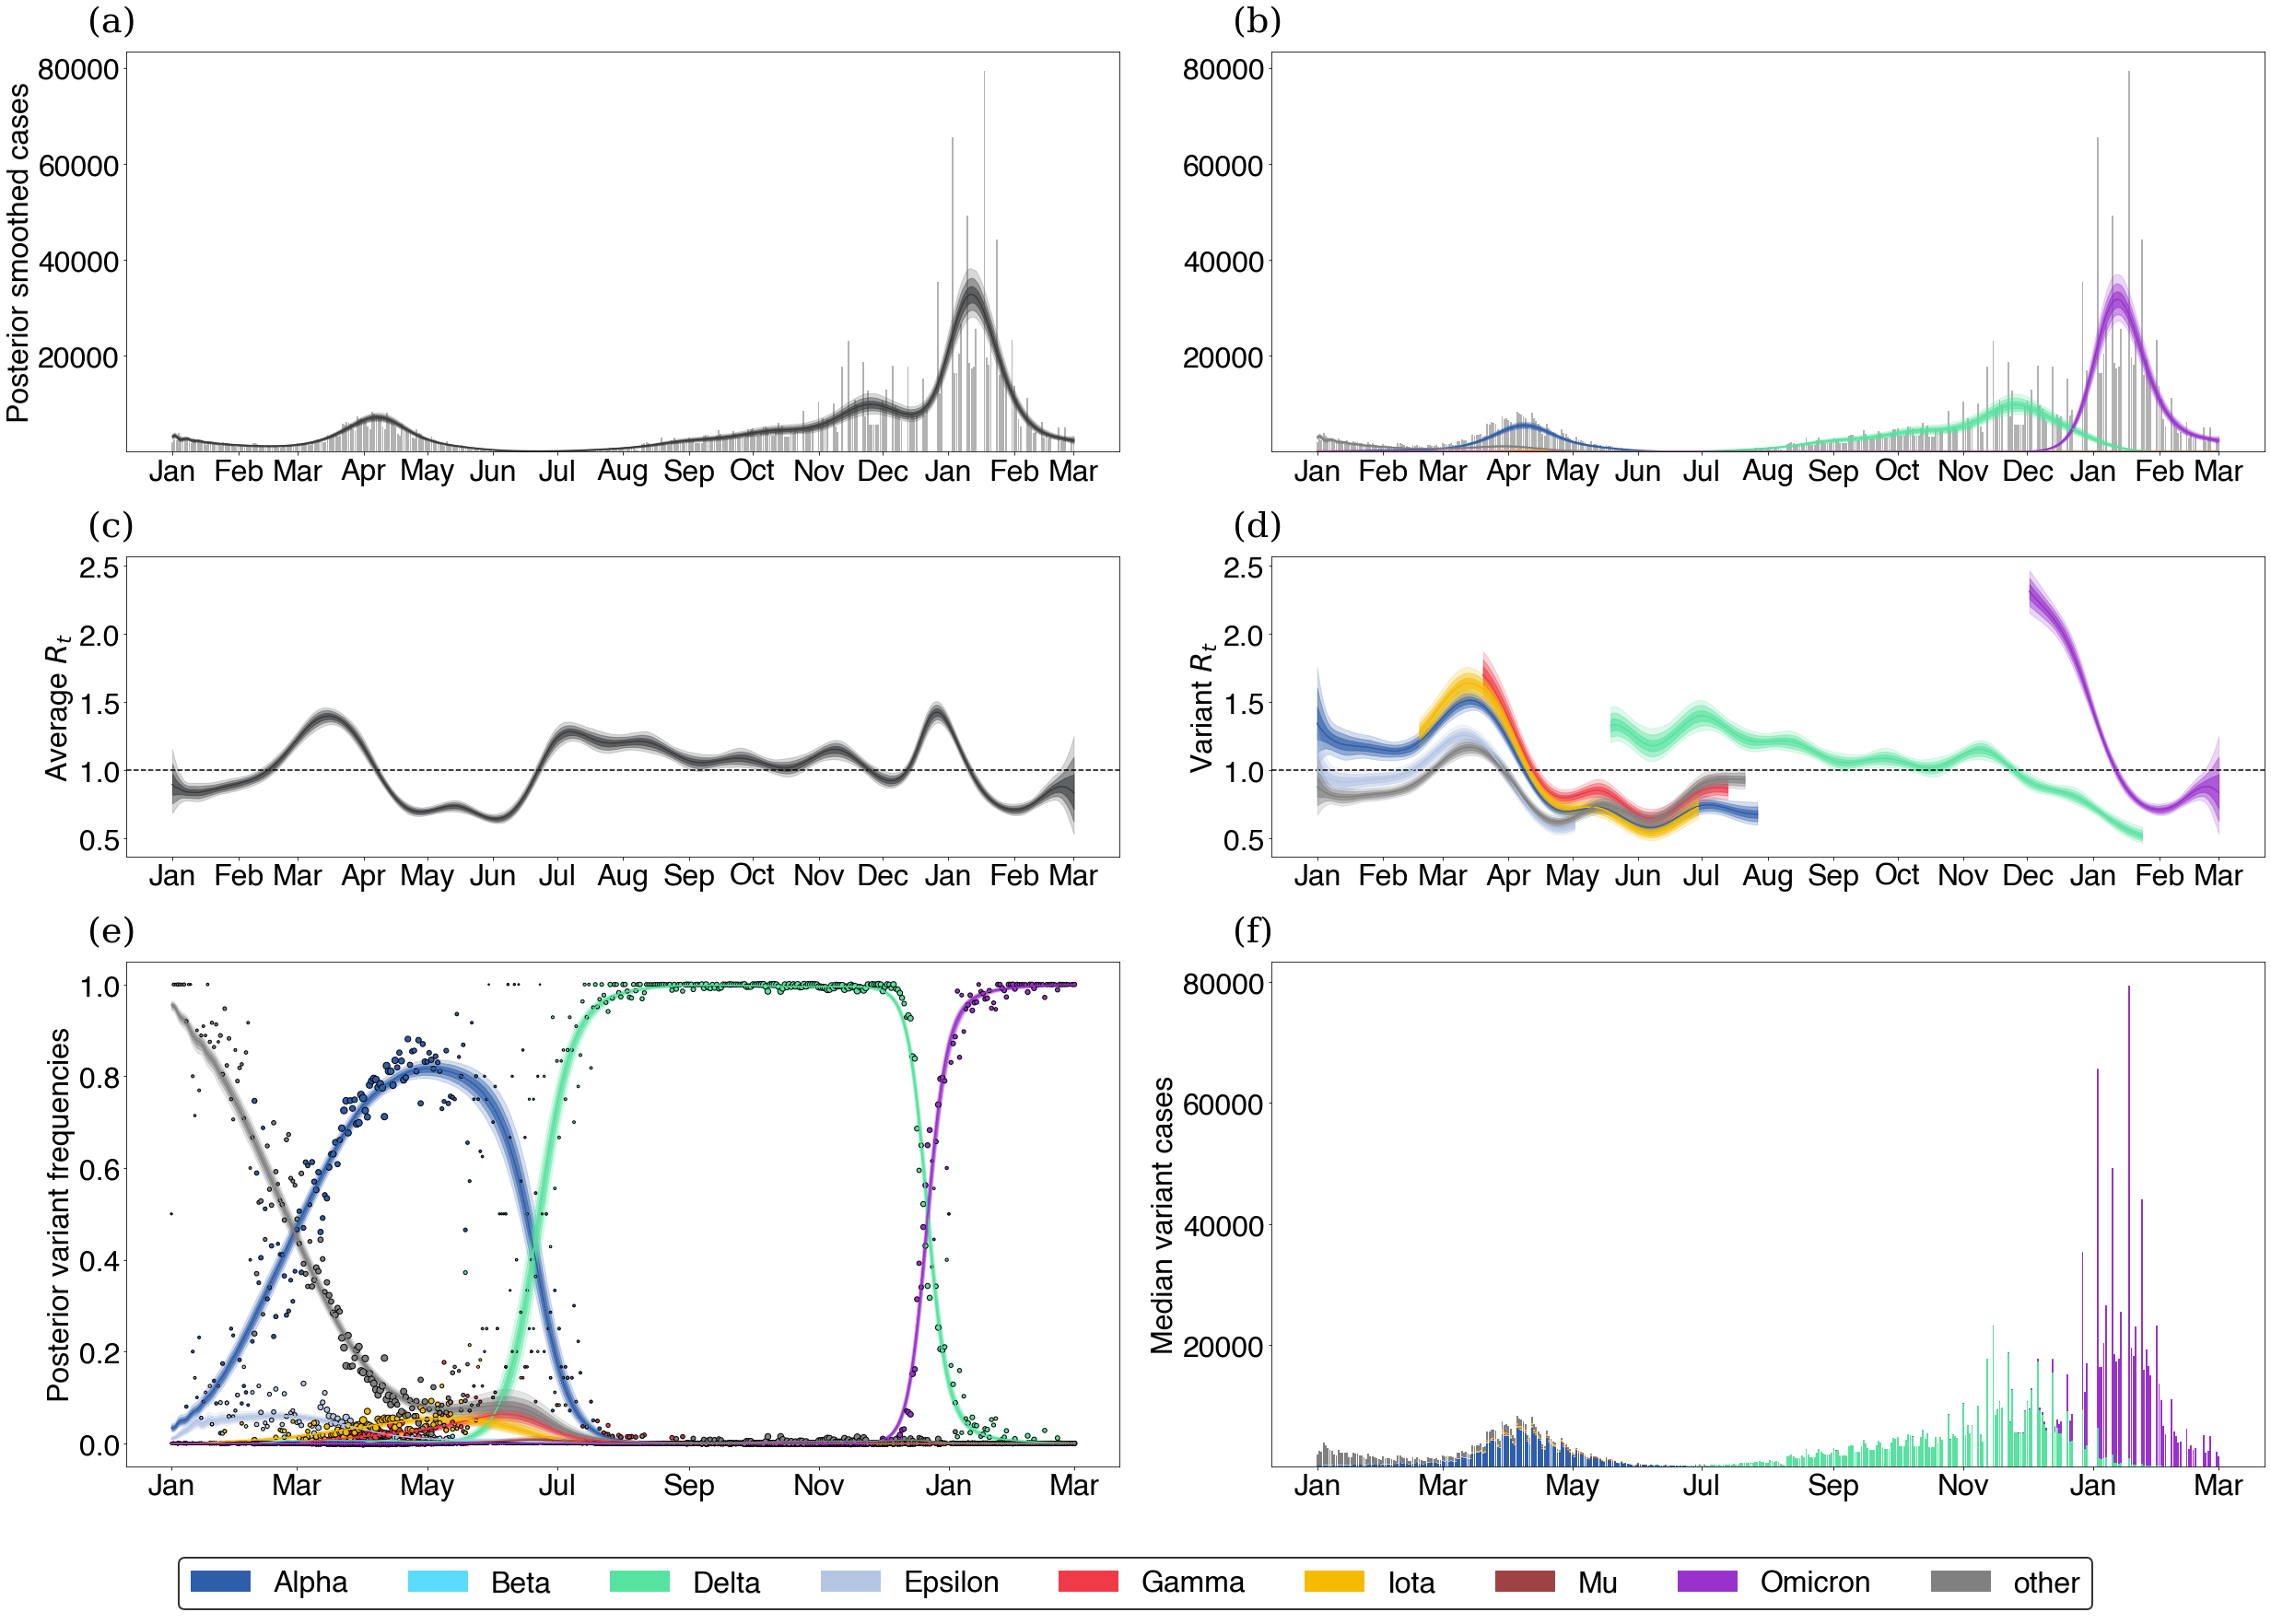
\includegraphics[width=\linewidth]{figs/GARW_rt_Michigan.png}
  \caption{\textbf{Fitting the GARW model to Michigan data.}}%
  \label{fig:GARW_rt_Michigan}
\end{figure}

\begin{figure}
  \centering
  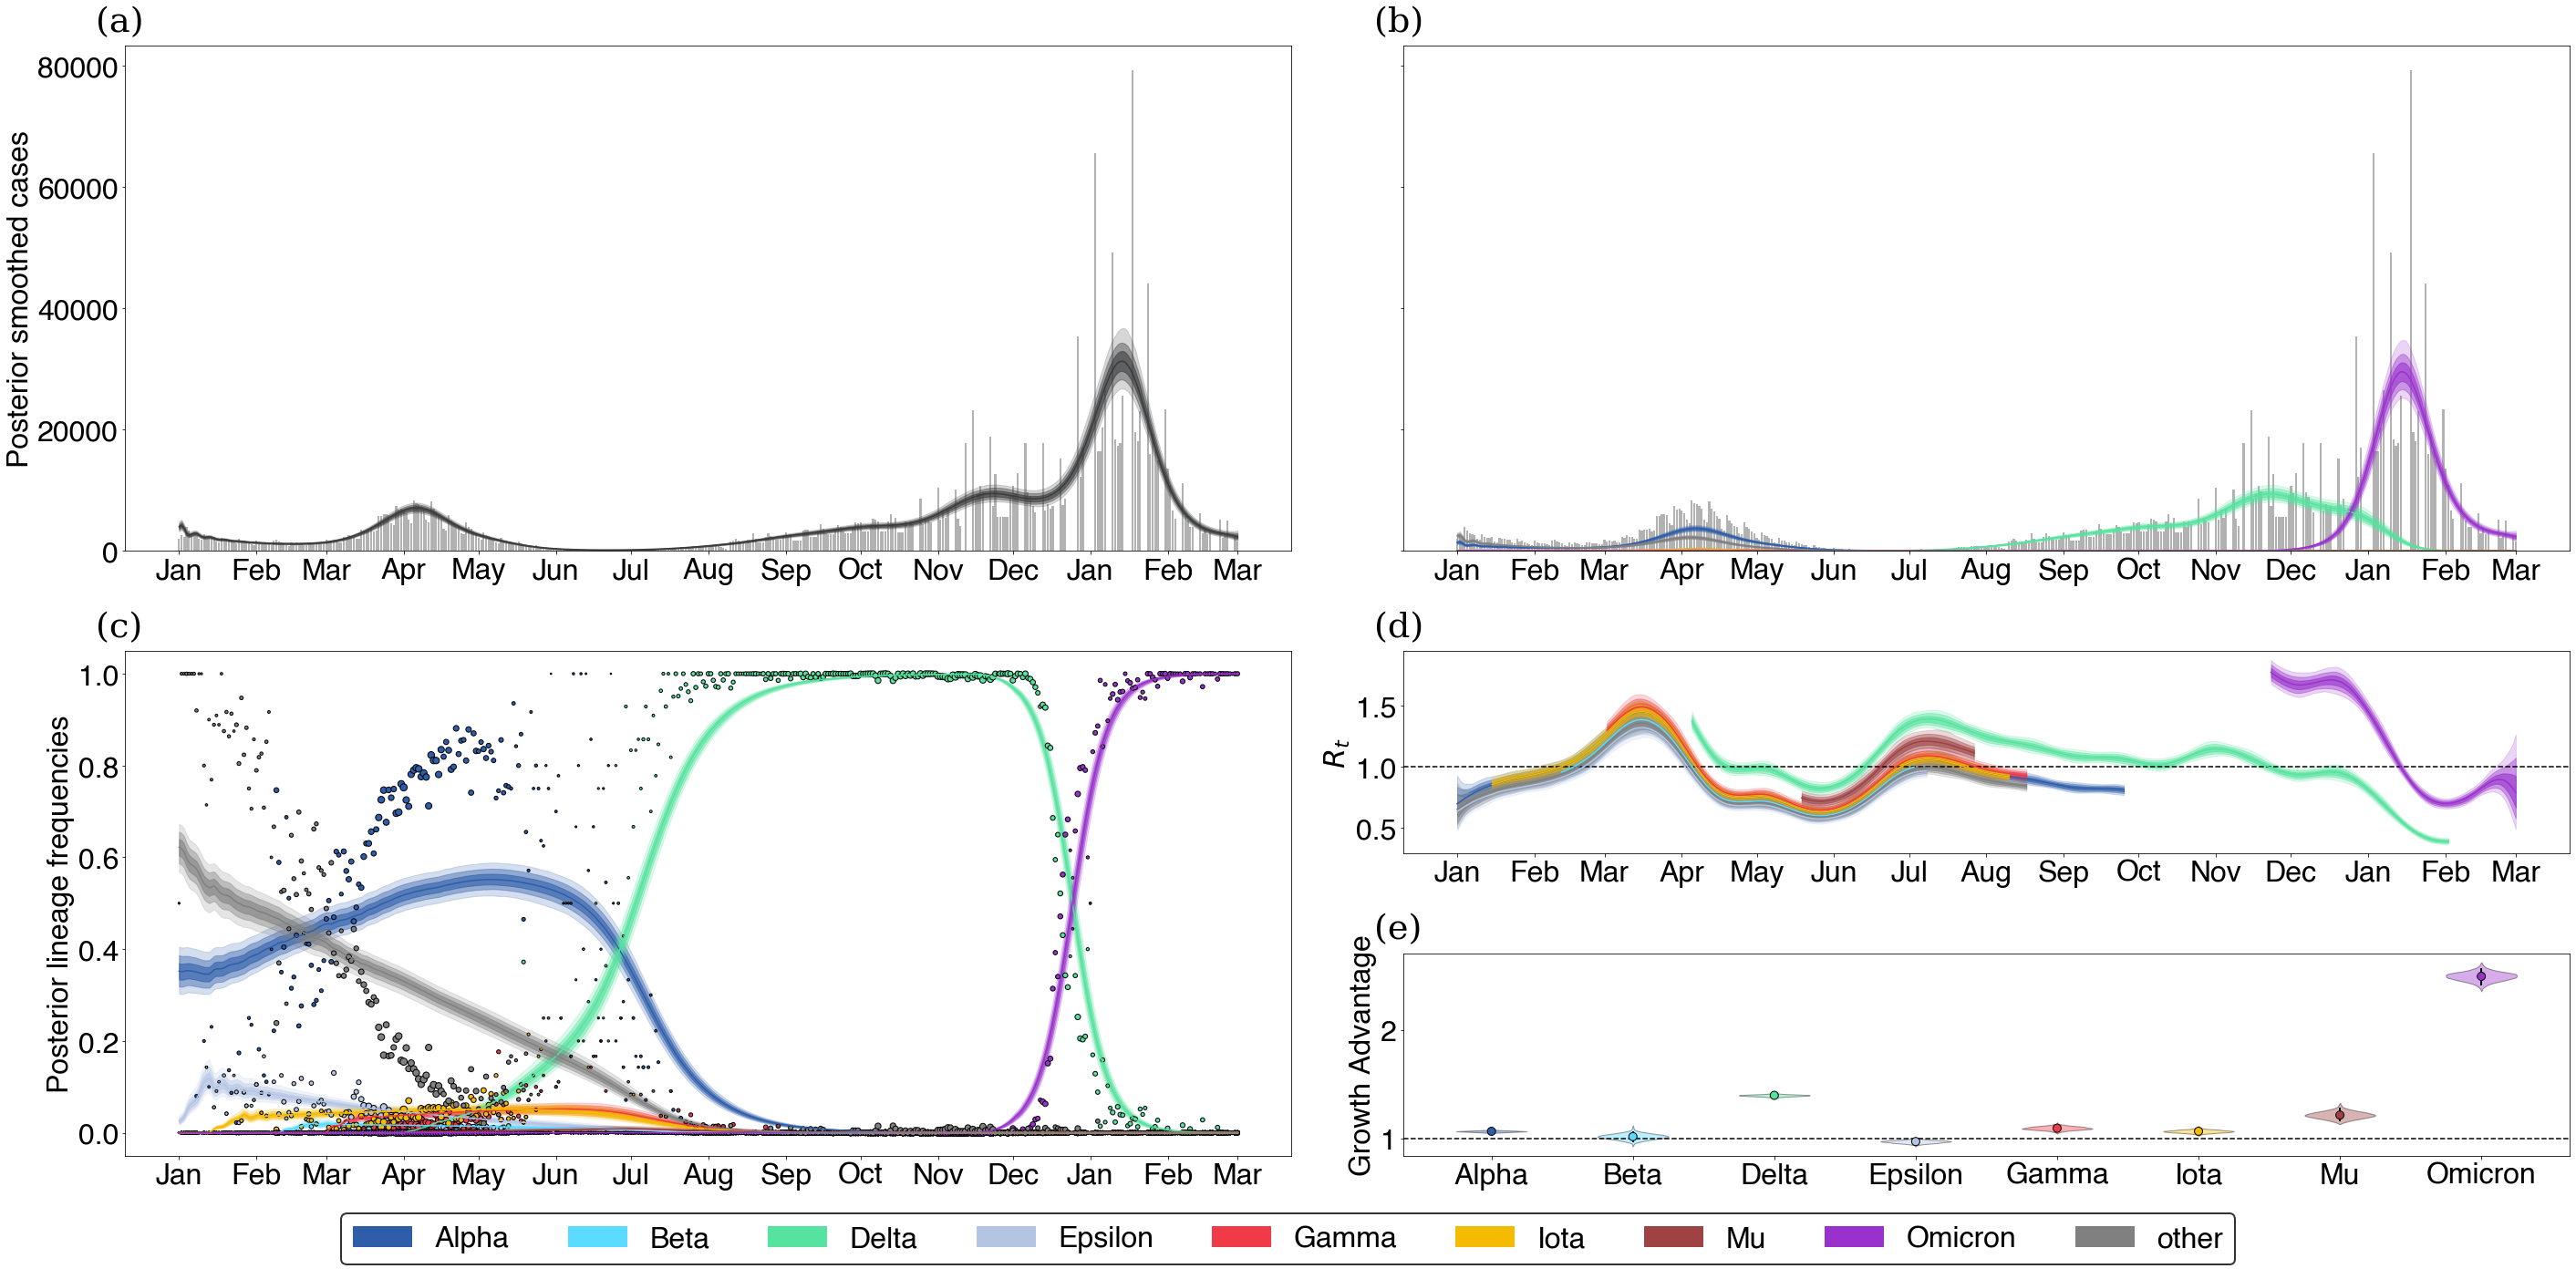
\includegraphics[width=\linewidth]{figs/fixed_growth_Michigan.png}
  \caption{\textbf{Fitting the fixed growth advantage model to Michigan data.}}%
  \label{fig:fixed_growth_Michigan}
\end{figure}

\begin{figure}
  \centering
  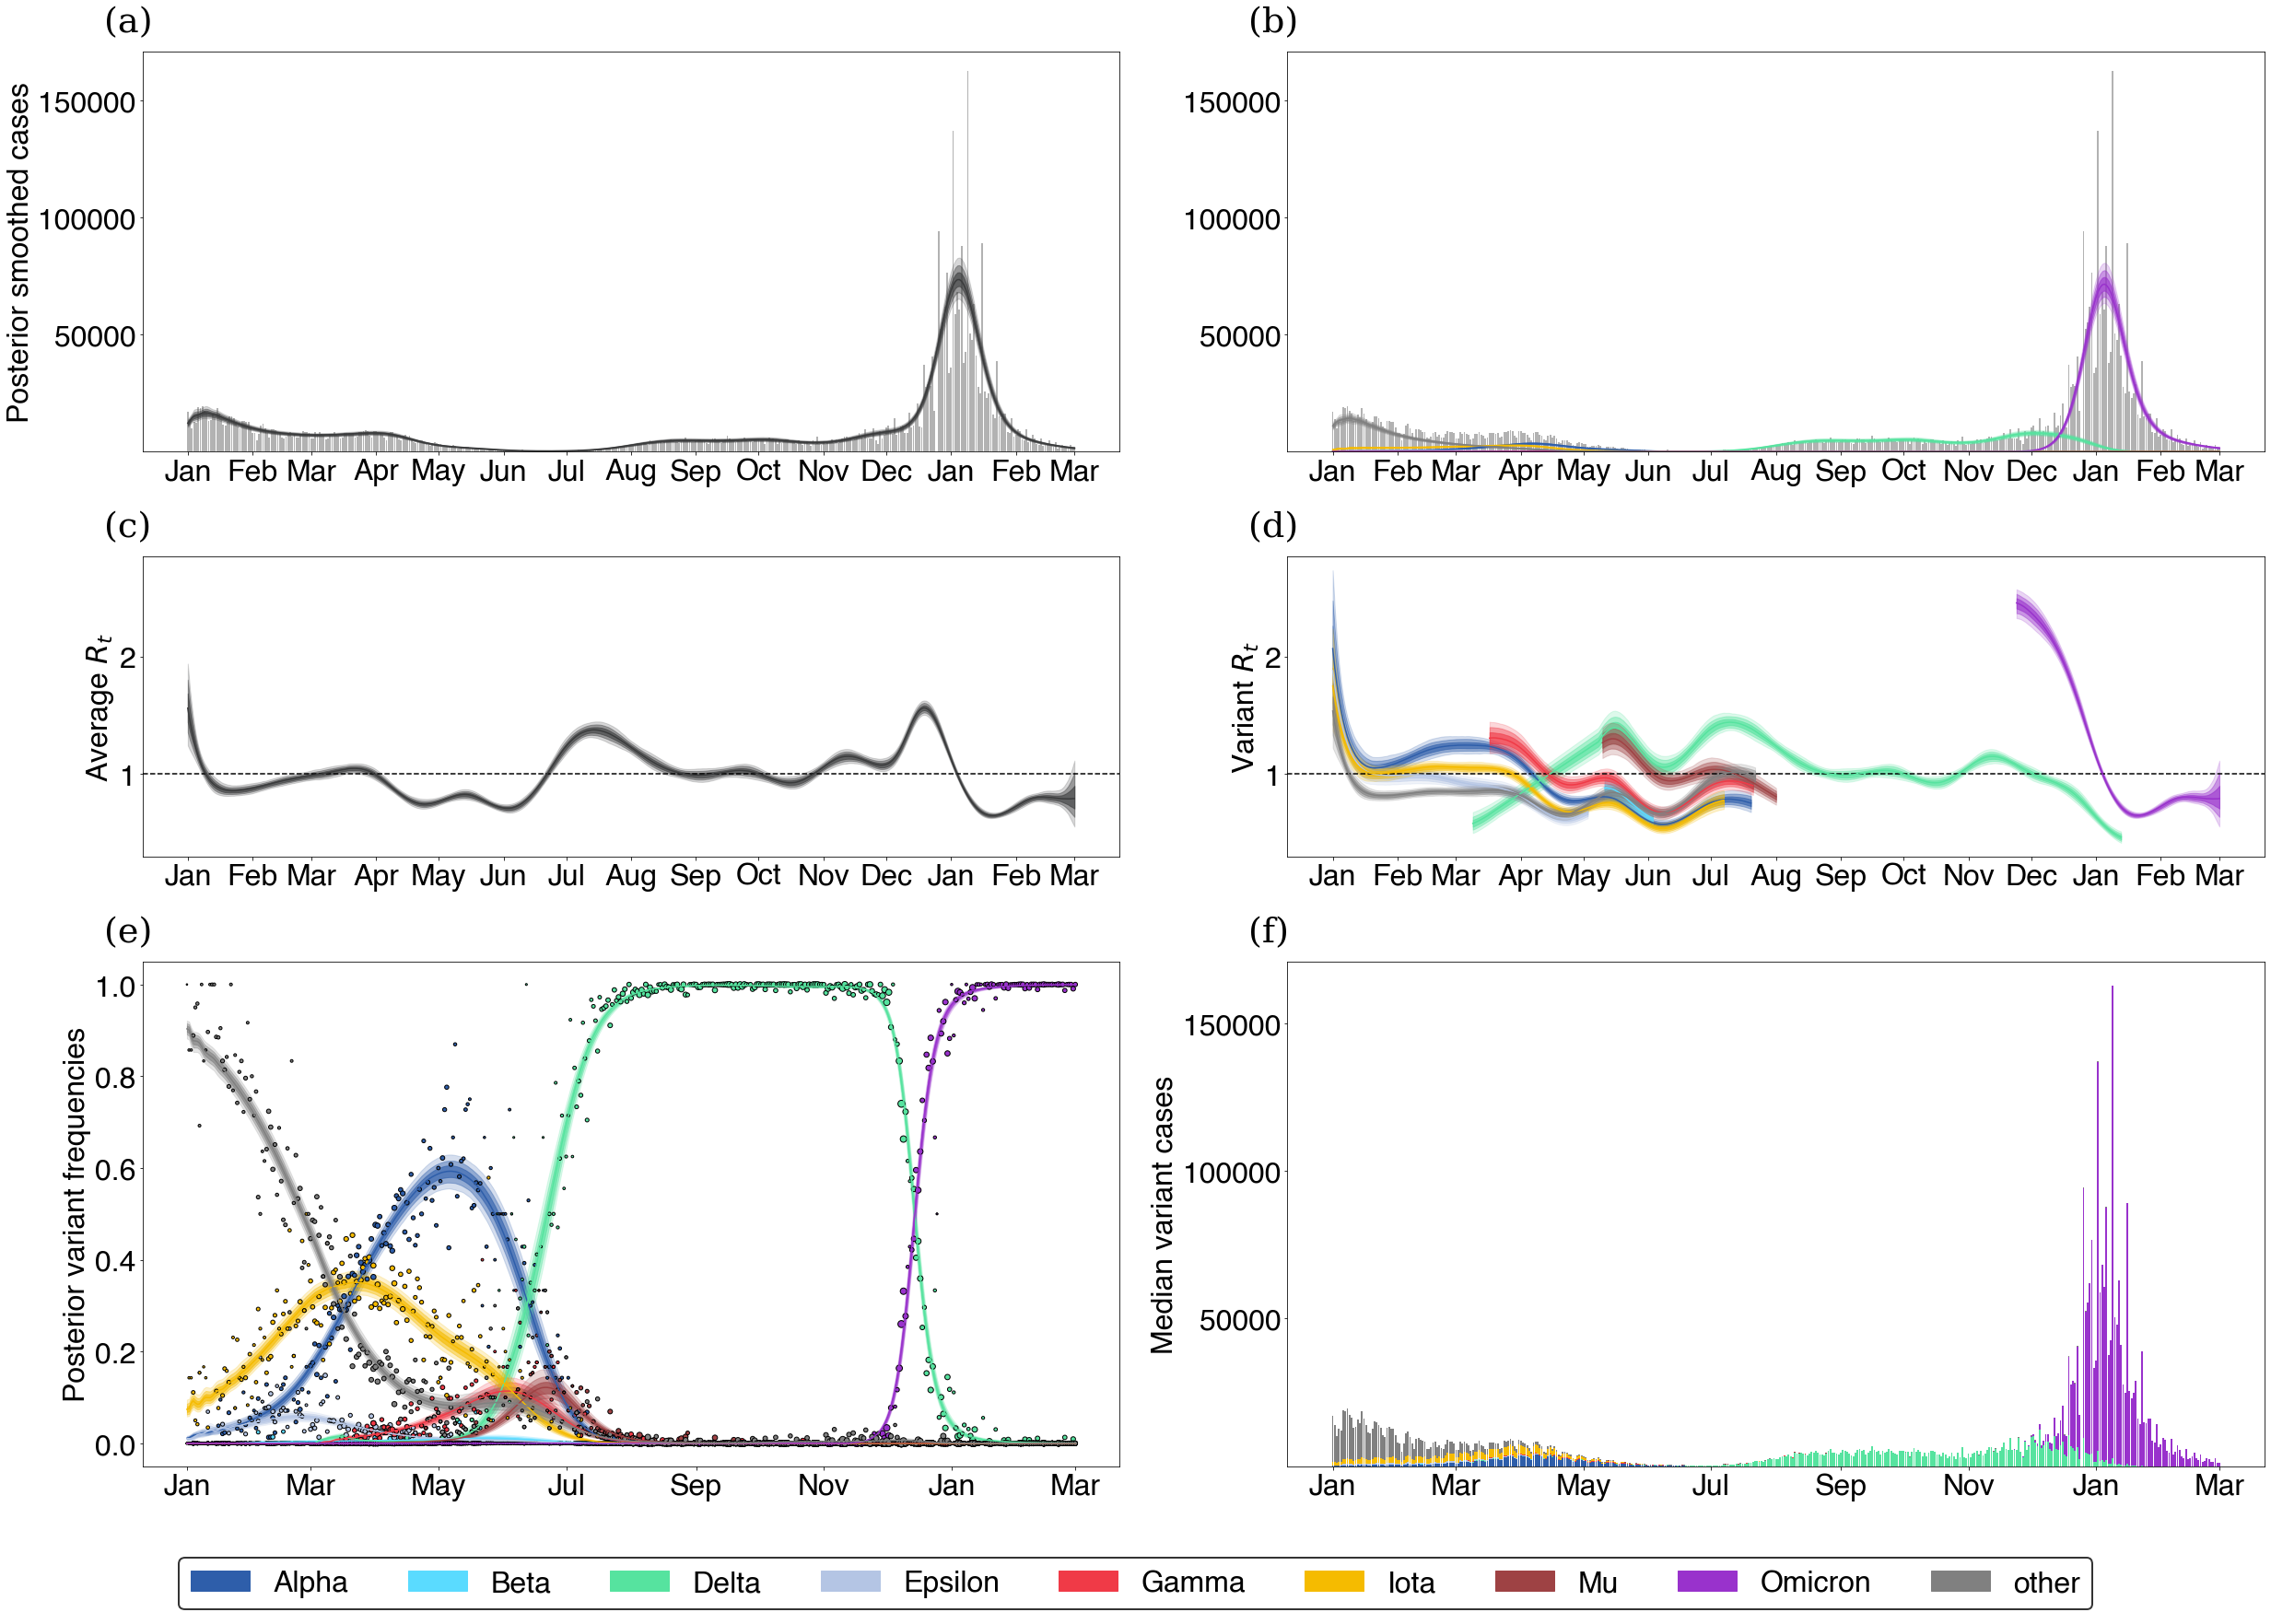
\includegraphics[width=\linewidth]{figs/GARW_rt_New-York.png}
  \caption{\textbf{Fitting the GARW model to New York state data.}}%
  \label{fig:GARW_rt_New-York}
\end{figure}

\begin{figure}
  \centering
  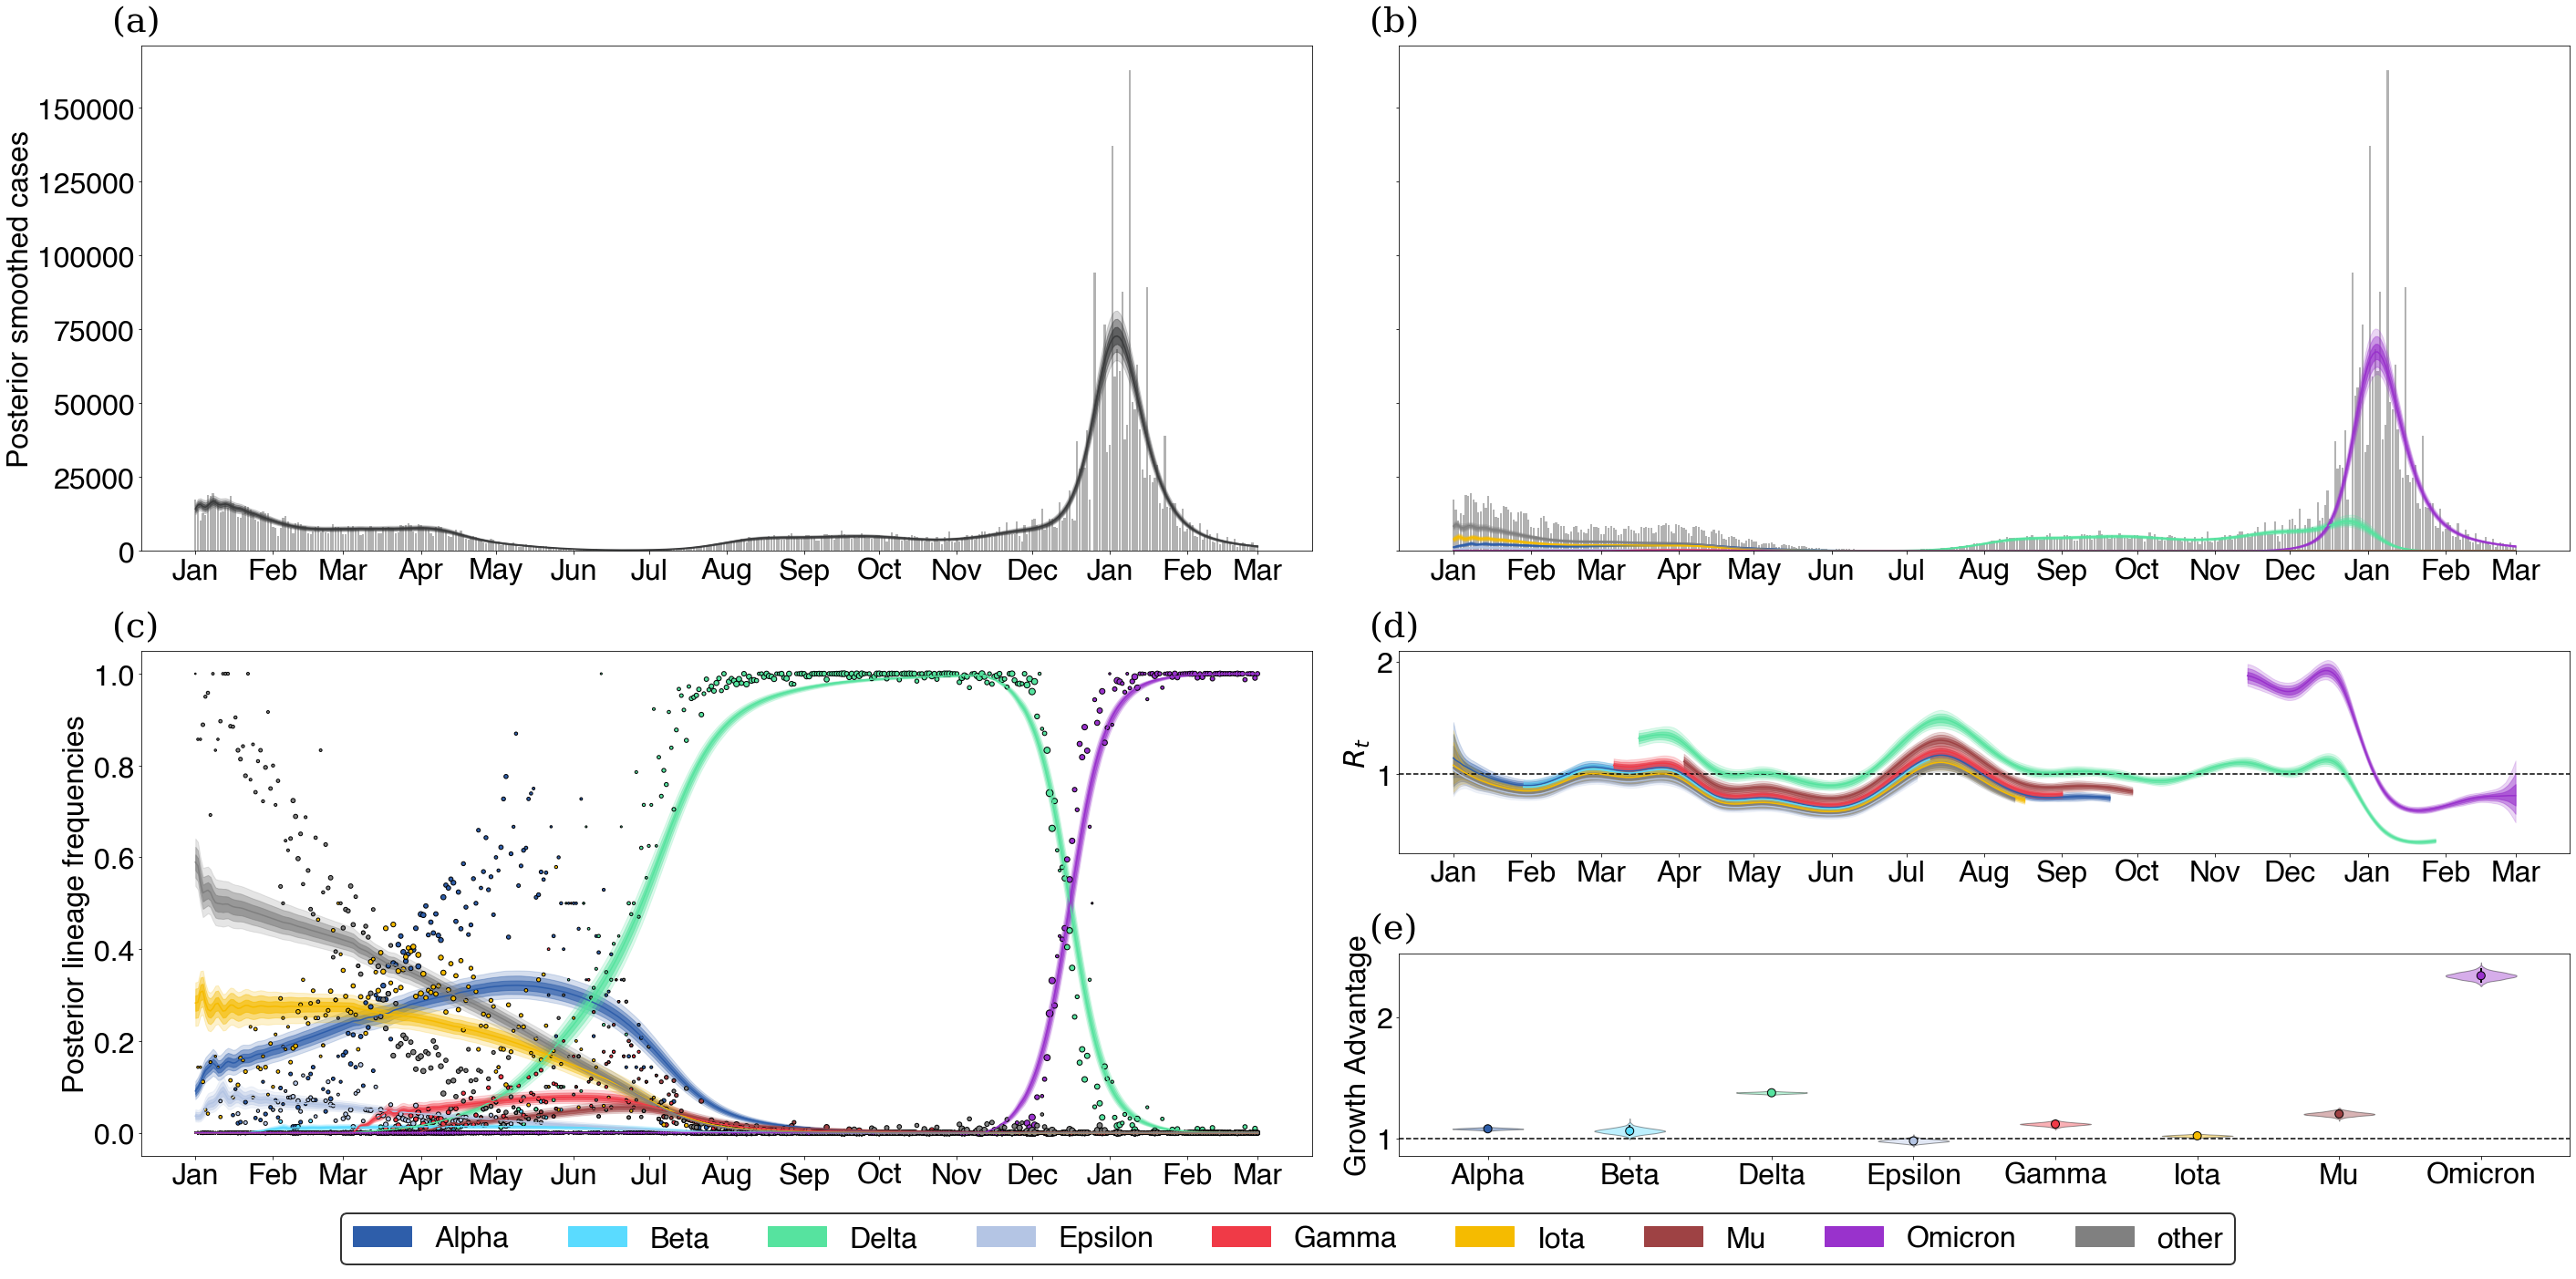
\includegraphics[width=\linewidth]{figs/fixed_growth_New-York.png}
  \caption{\textbf{Fitting the fixed growth advantage model to New York state data.}}%
  \label{fig:fixed_growth_New-York}
\end{figure}

\clearpage


\graphicspath{{./chapters/rt-from-frequency-dynamics/}}
\chapter{Supplementary Materials for Chapter 2} 

%TODO: Make sure we use supplementary results -> supplementary figures

\section{Supplementary Text}

\subsection*{Relationship to multinomial logistic regression}

Other papers have tried to infer growth advantages of variants from sequence data alone, we show that the multinomial logistic regression model typically used in these analysis is roughly equivalent to our fixed growth advantage model, but that inferring relative effective reproduction numbers between variants using multinomial logistic regression requires additional restrictions on the generation time.
Multinomial logistic regression typically models the probability of a given observation belong to class $v$ at time $t$ as
\begin{equation}
  f_{v}(t) = \frac{p_{v}\exp(\beta_{v} t)}{\sum_{1\leq u\leq V} p_{u}\exp(\beta_{u} t)}.
\end{equation}
For our purpose, we can assume this probability is equivalent to the true frequency of variant $v$ in the population and in this case, $p_{v}$ is considered to be related to the prevalence on variant $v$ in the population at $t=0$ and $\beta_{v}$ can be considered to be the growth advantage relative to a pivot class $u_{*}$ which has $\beta_{k_{*}} = 0$.
In order to see the connection between the above model and ours, we return to the original renewal equation of the form
\begin{equation}
  I(t) = R_{t}\int_{0}^{t} I(t-\tau) g(\tau).
\end{equation}
Assuming that $g$  is a point mass at a mean generation time $T_{g}$, we have that
\begin{equation}
  I(nT_{g}) = \left(\prod_{i=1}^{n} R_{iT_{g}}\right) I(0).
\end{equation}
Assuming that there are several variants following these same dynamics, we have that the frequency of a given variant $v$ can be written as
\begin{equation}
  f_{v}(nT_{g}) = \frac{I_{v}(nT_{g})}{\sum_{1\leq u \leq V} I_{u}(nT_{g})}.
\end{equation}
If we assume a constant growth advantage as in our model, we then have that $R_{t,v} = \Delta_{v} R_{t}$, so that
\begin{equation}
  f_{v}(nT_{g}) =  \frac{\Delta_{v}^{n} I_{v}(0)}{\sum_{1\leq u \leq V} \Delta_{u}^{n} I_{u}(0)}.
\end{equation}
Writing $\Delta_{v} = \exp(\delta_{v})$ and $t = n T_{g}$, allows us to see that
\begin{equation}
  f_{v}(t) = \frac{I_{v}(0) \exp(\frac{\delta_{v}}{T_{g}} t)}{\sum_{1\leq u \leq V}I_{u}(0) \exp(\frac{\delta_{u}}{T_{g}} t)}.
\end{equation}
By fixing one pivot class so that $I_{u_{*}} = 1$ and $\delta_{u_{*}} / T_{g} = 0$, we can identify our model with the multinomial logistic regression by relating the parameters as

\begin{align}
  \delta_{v} &= \beta_{v}T_{g}\\
  I_{v}(0) &= p_{v}.
\end{align}

This shows that the multinomial logistic regression functions similarly to our fixed growth advantage model except with the additional assumption that the generation time is a point mass at $T_{g}$.
This assumption additionally allows us to relate the epidemic growth rate $r$ and the effective reproduction number as $R = \exp(r T_{g})$ \cite{Wallinga2006}.
Therefore, by further assuming that the variant infections are exponentially growing with rates $r_{v}$, we can then identify $\beta_{v} = r_{v} - r_{u_{*}}$.
This means that the relative effective reproduction number for any two variants can be written as
\begin{align*}
\ln \left( \frac{R_{t,v}}{R_{t,u}} \right) = (\beta_{v} - \beta_{u}) T_{g}.
\end{align*}

\begin{figure}
  \centering
  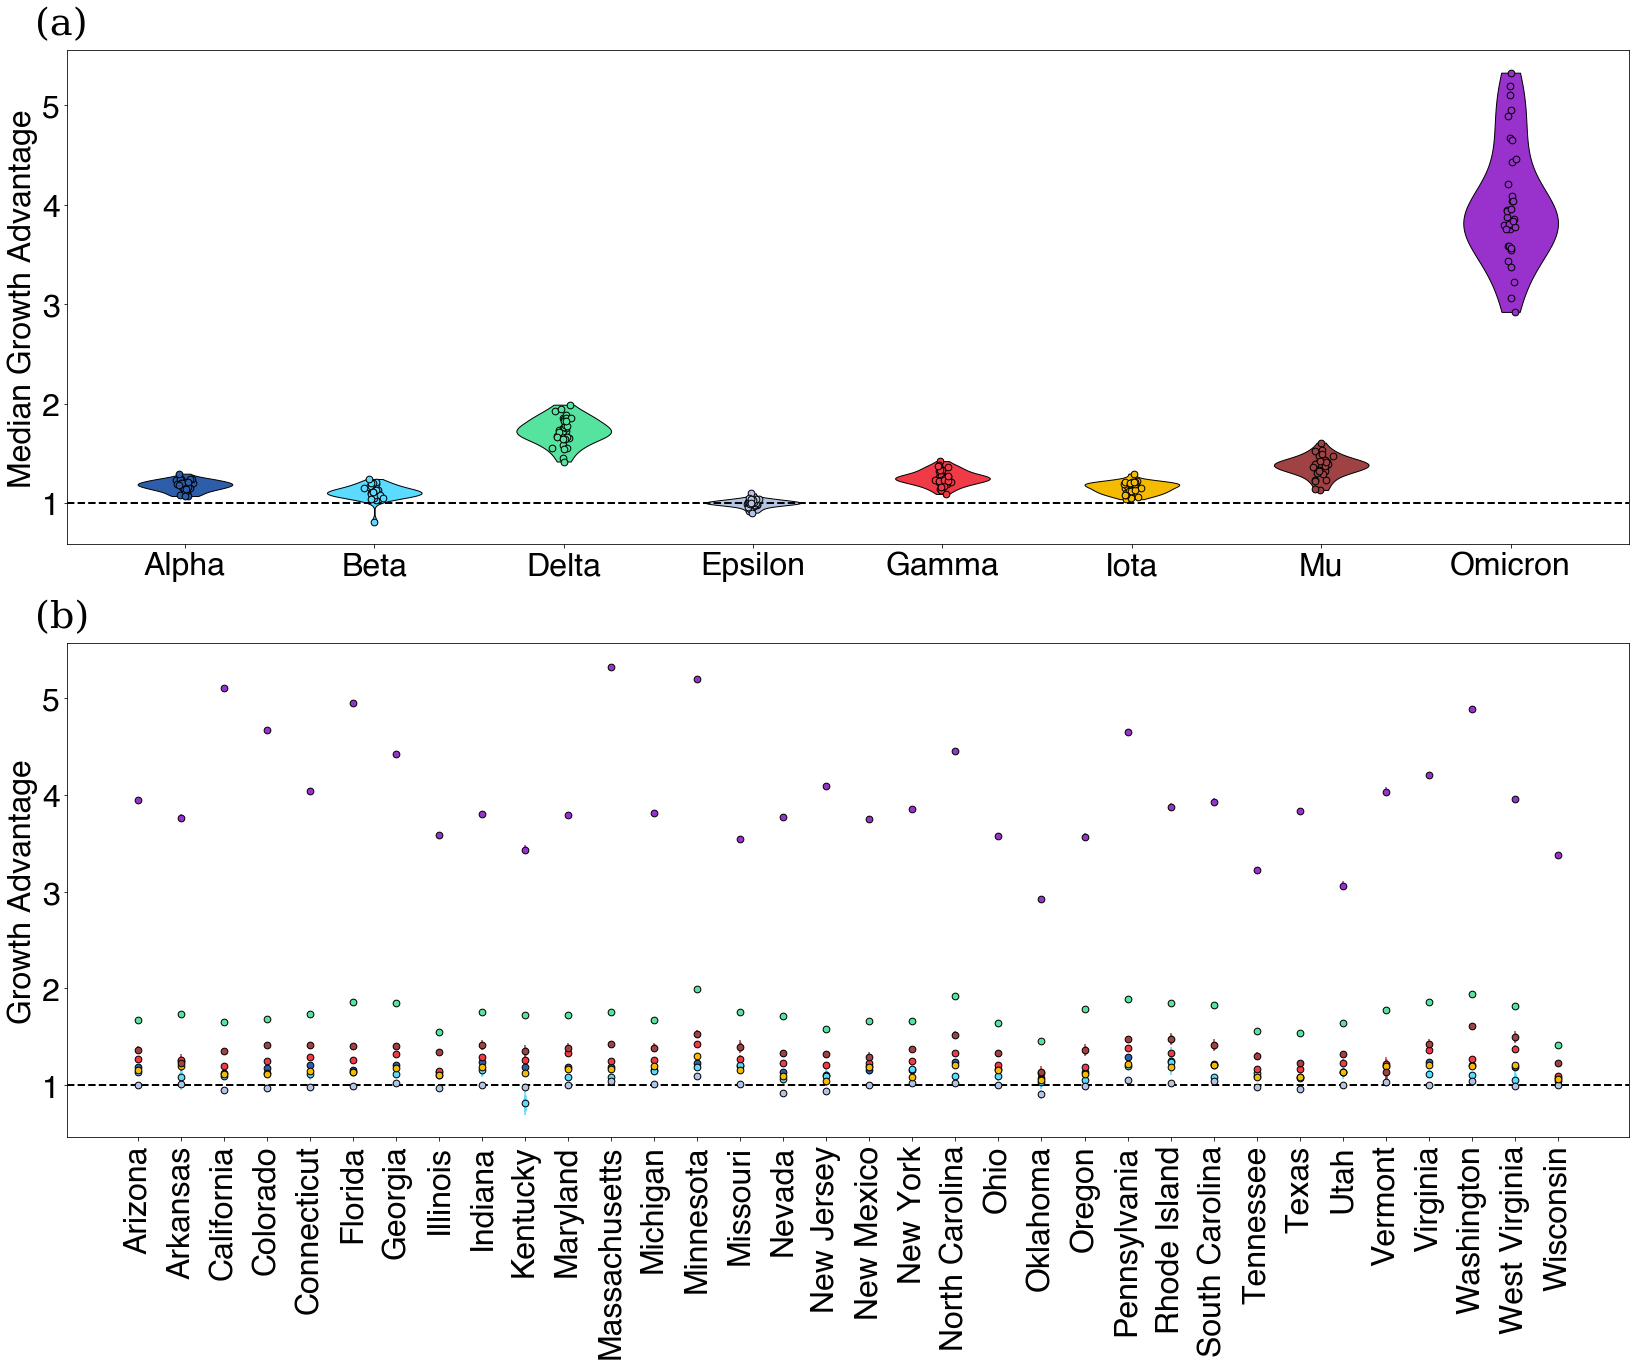
\includegraphics[width=\linewidth]{figs/fig_MLR_growth_advantages_supp.png}
  \caption{Estimating variant growth advantages in various states using Multinomial Logistic Regression model assuming generation time $T_{g} = 5.2$.
  (a) Growth advantages visualized by state.
  (b) Same as (a) but grouped by variant.}%
  \label{fig:MLR_growth_advantages}
\end{figure}

\newpage

\subsection*{Relating epidemic growth rates to relative effective reproduction numbers}

An important relationship of interest is between the epidemic growth rate of an epidemic and its effective reproduction number.
In the case of our analysis, we are particularly interested in the effect of generation time assumptions on estimated variant-specific effective reproduction numbers.
First, notice that the effective reproduction number and the epidemic growth rate of an epidemic are related by
\begin{align*}
R_{t} = \frac{1}{\int_{0}^{\infty} \exp(-r\tau)g(\tau)d\tau} = \frac{1}{M_{g}(-r)}
\end{align*}
according to the Lotka-Euler equation \cite{Wallinga2006} where $r$ is the epidemic growth rate and $M_{g}$ is the moment-generating function of the generation time $g$.

This allows us to write the relative reproduction number of two variants $v$ and $u$ as a function of their epidemic growth rates, so that
\begin{align*}
\frac{R_{t,v}}{R_{t,u}} = \frac{M_{g}(-r_{u})}{M_{g}(-r_{v})}.
\end{align*}

We'll consider three common generation time assumptions. First, we consider the case where the generation time is a point mass at $T_{g}$. In which case, $M_{g}(-r) = \exp(-r T_{g})$ and we recover the relationship
\begin{align*}
R_{t,v} = \exp(r_{v}T_{g}).
\end{align*}

In this case, the relative effective reproduction number will depend on only the difference between the epidemic growth rates and therefore, is commonly used when converting estimated growth advantages to relative reproduction numbers in the case of logistic growth models.

Second, we consider the case where the generation time is an exponential distribution with mean $T_{g}$. This assumption is often implicit and common in models of infectious diseases such as ODEs and their stochastic variants. Using the corresponding moment-generating function, we see that
\begin{align*}
R_{t,v} = 1 + r_{v} T_{g}
\end{align*}

Next, we consider the Gamma distributed generation times with mean $T_{g}$ and standard deviation $s$.
This is often used in models of infectious diseases via the chain trick in which multiple compartments are chained together to obtain non-exponential generation times or infectious periods.
Re-parameterizing the Gamma distribution in terms of its mean and standard deviation and using its moment generating function, we have that
\begin{align*}
R_{t,v} = \left(1 + r_{v}  \left(\frac{s^{2}}{T_{g}}\right) \right)^{T_{g}^{2} / s^{2}}.
\end{align*}

From this equation, we can see that increases in the mean of the generation time of $v$ leads to decreasing estimates of $R_{t,v}$ during epidemic decline ($r_{v} < 0$) and increased estimates during epidemic growth ($r_{v} > 0$) assuming $r_{v}$ and $s$ are fixed.
Additionally, increases in the standard deviation will generally lead to lower inferred variant advantages.
This effect is also visualized in Figure \ref{fig:generation_time_sensitivity}.

\paragraph{Variant growth-advantages are sensitive to generation time}%

In the case where we have two variants $u, v$ with Gamma-distributed generation times with means $T_{u}, T_{v}$ and standard deviations $s_{u}, s_{v}$ respectively, we can then write the relative effective reproduction number of $v$ over $u$ as
\begin{align*}
\frac{R_{t,v}}{R_{t,u}} = \frac{\left[1 + r_{v}  \left(\frac{s_{v}^{2}}{T_{v}}\right)\right]^{T_{v}^{2} / s_{v}^{2}}}{\left[1 + r_{u} \left(\frac{s_{u}^{2}}{T_{u}}\right)\right]^{T_{u}^{2} / s_{u}^{2}}}.
\end{align*}
It follows that increases in the mean of the generation time of $v$ leads to decreasing inferred variant advantages during epidemic decline and increased advantages during epidemic growth when all quantities are fixed.
On the other hand, increases in the standard deviation will generally lead to lower inferred variant advantages.

Taking a logarithm, we can also evaluate the sensitivity of our inferred growth advantages from our fixed growth advantage model with respect to the generation time assuming it is Gamma distributed as
\begin{align*}
 \delta_{v}  = \ln \left( \frac{R_{t,v}}{R_{t,0}} \right) = \left( \frac{T_{g}^{2}}{s^{2}} \right)  \ln \left( \frac{1 + r_{v}  \left(\frac{s^{2}}{T_{g}}\right)}{1 + r_{0} \left(\frac{s^{2}}{T_{g}}\right) } \right).
\end{align*}
As the log of the relative effective reproduction number, the behavior here is analogous to that discussed above when the mean $T_{g}$ and standard deviation $s$ are changed.
This effects of varying mean and standard deviation are illustrated in Figure \ref{fig:growth_advantage_sensitivity}.
Although the effective reproduction number and the growth advantage appear to have strong dependence on generation time parameters, we find that the epidemic growth rate $r$ is more robust to changes in generation time (see Figure \ref{fig:little_r_sensitivity}).

The cases of exponential and Gamma-distributed generation times highlight that for non-deterministic generation times there is no guarantee that the relative effective reproduction number depends on only the difference in epidemic growth rates.
In fact, these estimates based on the deterministic generation times correspond to the case in which the standard deviation shrinks zero, they are likely overestimates of variant advantages given the observed variation in the serial interval of SARS-CoV-2 infections.

\paragraph{Fixed growth advantages become time-varying under generation time misspecification}

We'll now consider the case where there is a true fixed-variant growth advantage. Suppose for a two-variant system that $\delta$ is the constant (log) growth advantage of the variant virus over the wildtype under the variant generation time $g_{T}$, so that $\delta = \ln \left( R_{t,v}^{g_{T}} / R_{t, wt}^{g_{T}} \right)$.
Here subscripts denote the generation time used when computing $R_{t}$.

Under the misspecified variant generation time $g_{M}$, we can then write the inferred growth advantage as
\begin{align*}
  \delta_{M} &= \ln \left( \frac{R_{t,v}^{g_{M}}}{R_{t, wt}^{g_{T}}} \right) = \ln \left(\frac{R_{t,v}^{g_{M}}}{R_{t,v}^{g_{T}}}\right) + \delta.
\end{align*}

In general, the term inside the log is non-constant meaning that fixed variant growth advantages under one generation time become non-constant under generation time specification.

\begin{figure}
  \centering
  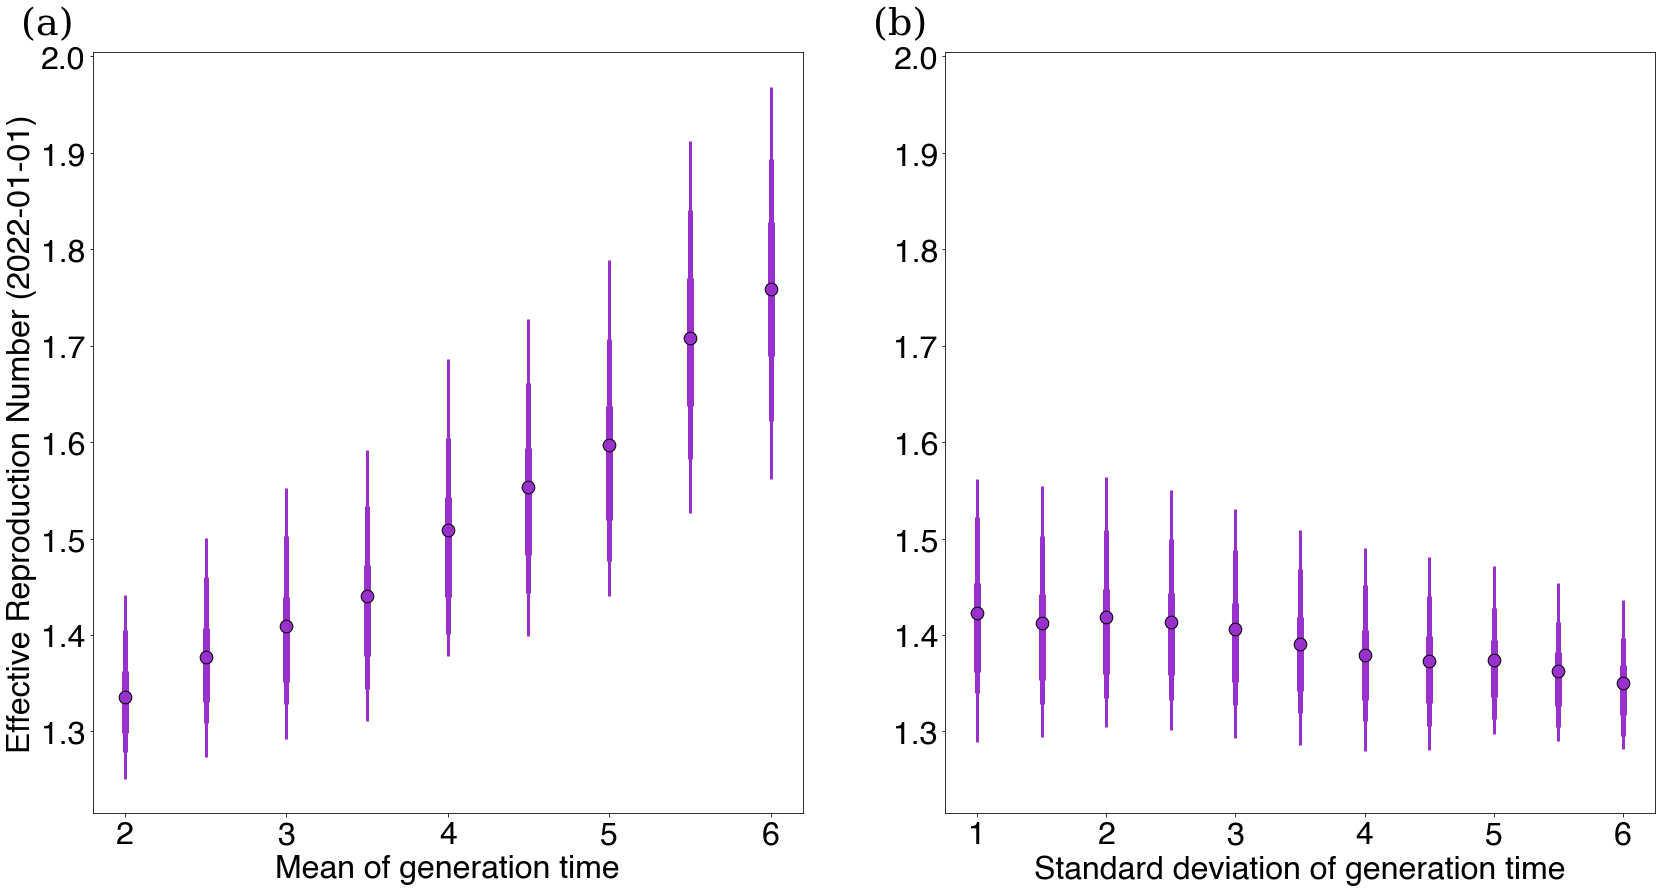
\includegraphics[width=\linewidth]{figs/generation_time_sensitivity.png}
  \caption{\textbf{Sensitivity of effective reproduction number to changes in generation time.}
(a) We vary the mean of Omicron generation time keeping a constant standard deviation 1.2 and plot against effective reproduction number estimates for Omicron in Washington state on February 1st, 2022 using our GARW model.
(b) The same as (a), but we instead vary the standard deviation of Omicron generation time keeping a constant mean 3.1.}%
  \label{fig:generation_time_sensitivity}
\end{figure}

\begin{figure}
  \centering
  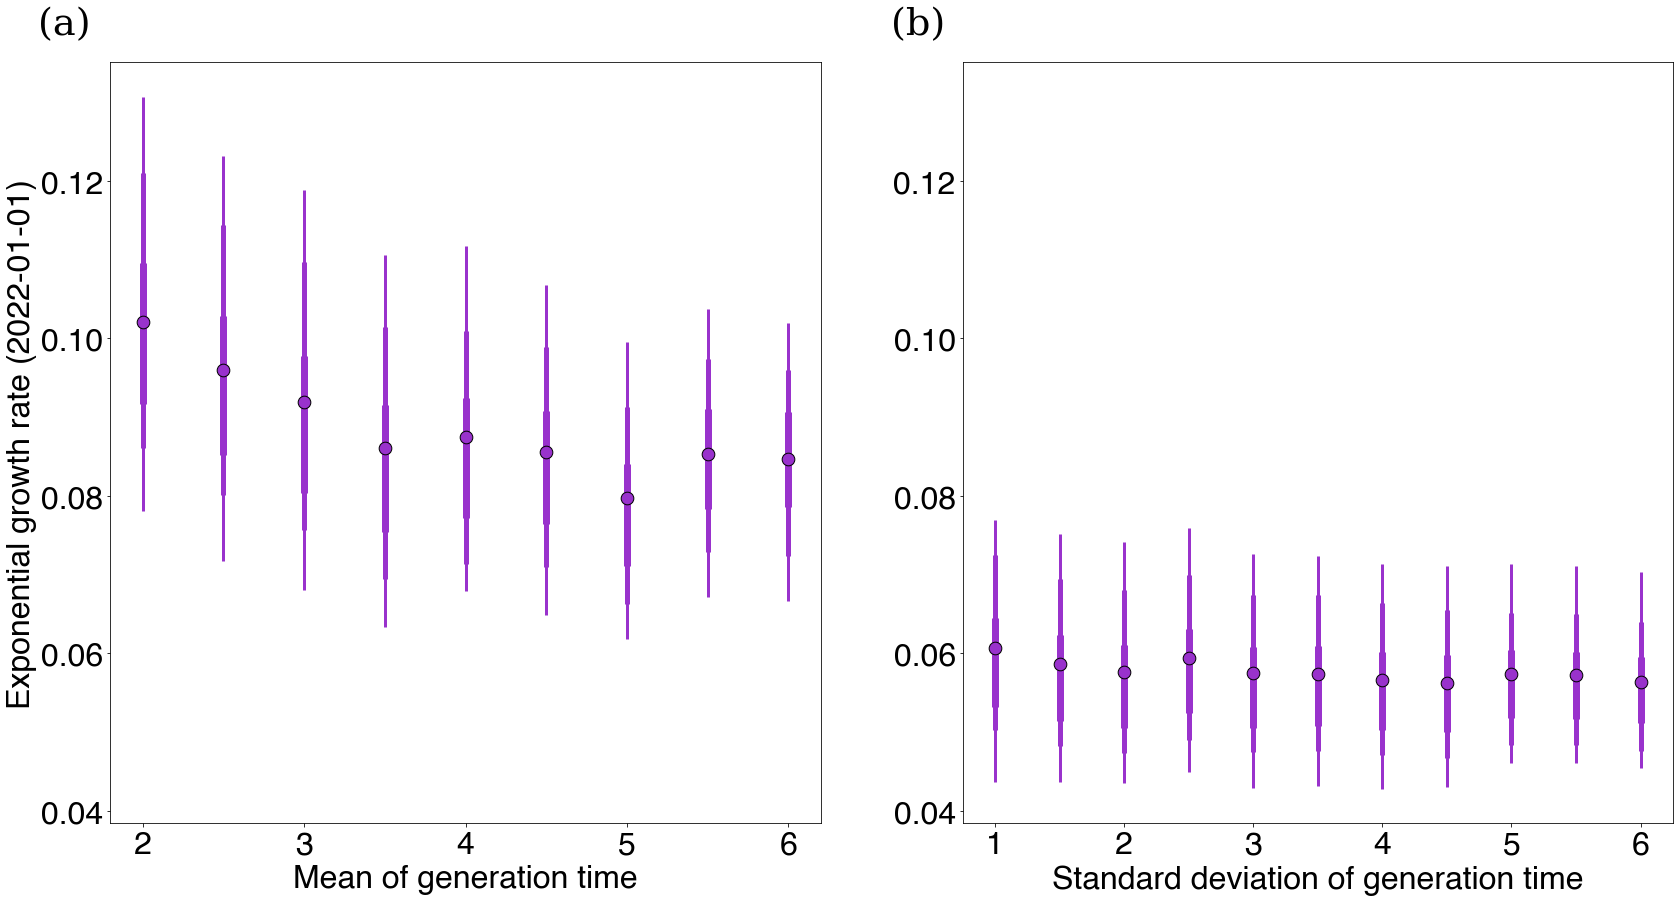
\includegraphics[width=\linewidth]{figs/little_r_sensitivity.png}
  \caption{\textbf{Sensitivity of epidemic growth rates to changes in generation time.}
(a) We vary the mean of Omicron generation time keeping a constant standard deviation 1.2 and plot against exponential growth rates for Omicron in Washington state on February 1st, 2022 using our GARW model and assuming a Gamma-distributed generation time.
(b) The same as (a), but we instead vary the standard deviation of Omicron generation time keeping a constant mean 3.1. }%
  \label{fig:little_r_sensitivity}
\end{figure}

\begin{figure}
  \centering
  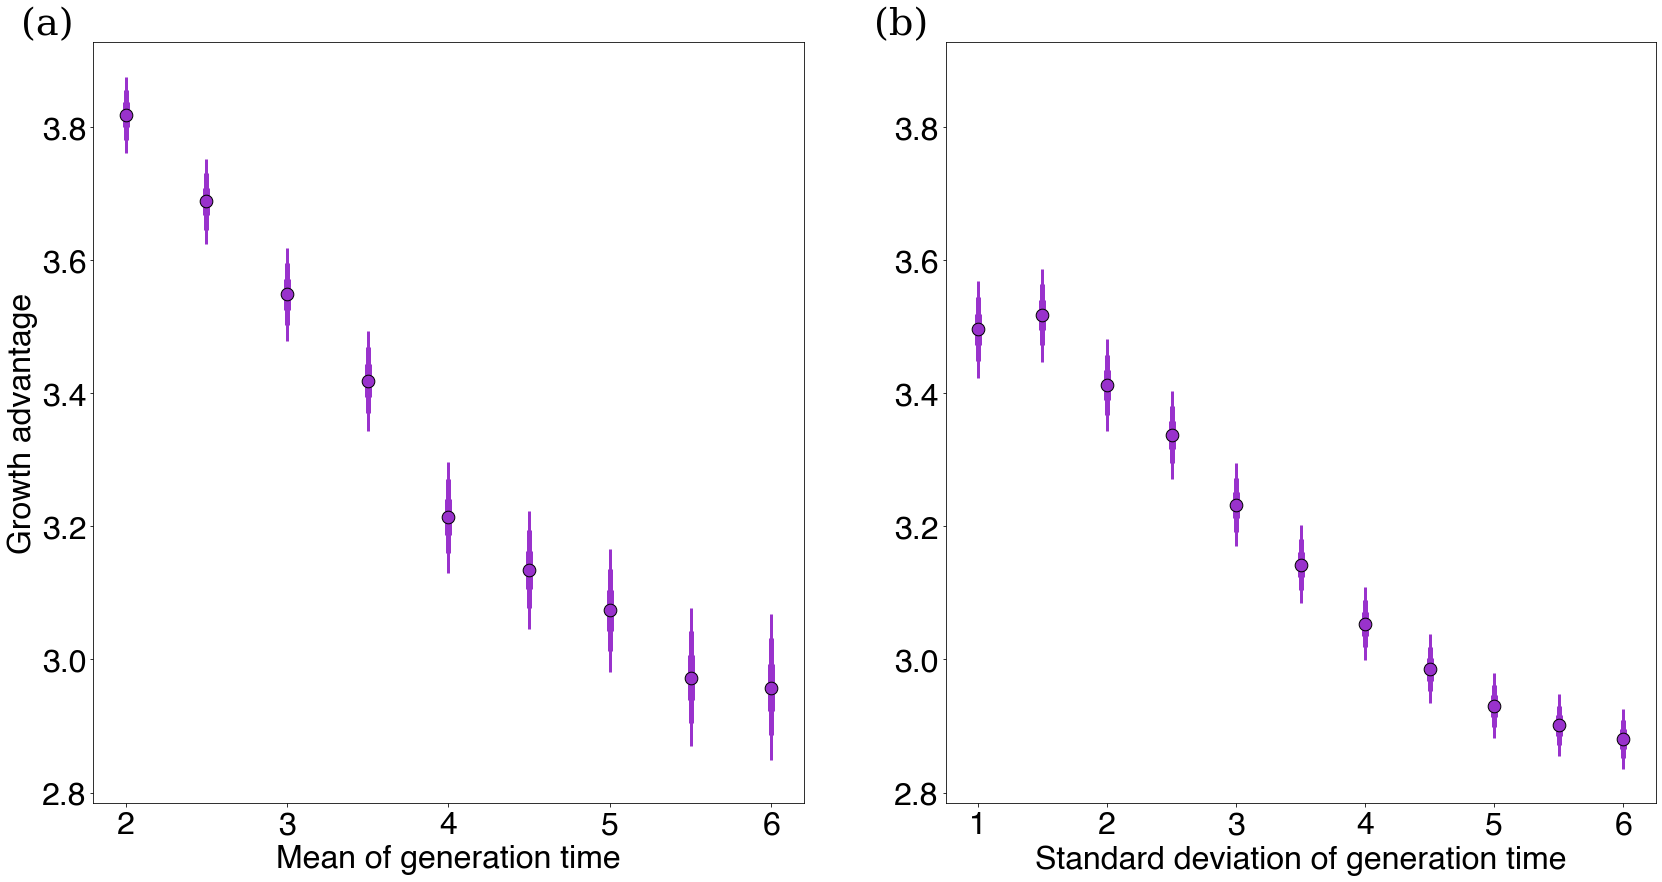
\includegraphics[width=\linewidth]{figs/growth_advantage_sensitivity.png}
  \caption{\textbf{Sensitivity of growth advantages to changes in generation time.}
(a) We vary the mean of Omicron generation time keeping a constant standard deviation 1.2 and plot against exponential growth rates for Delta in Washington state on July 1st, 2021 using our fixed growth model.
(b) The same as (a), but we instead vary the standard deviation of Omicron generation time keeping a constant mean 3.2.}%
  \label{fig:growth_advantage_sensitivity}
\end{figure}

\section{Supplementary Figures}

\begin{figure}
  \centering
  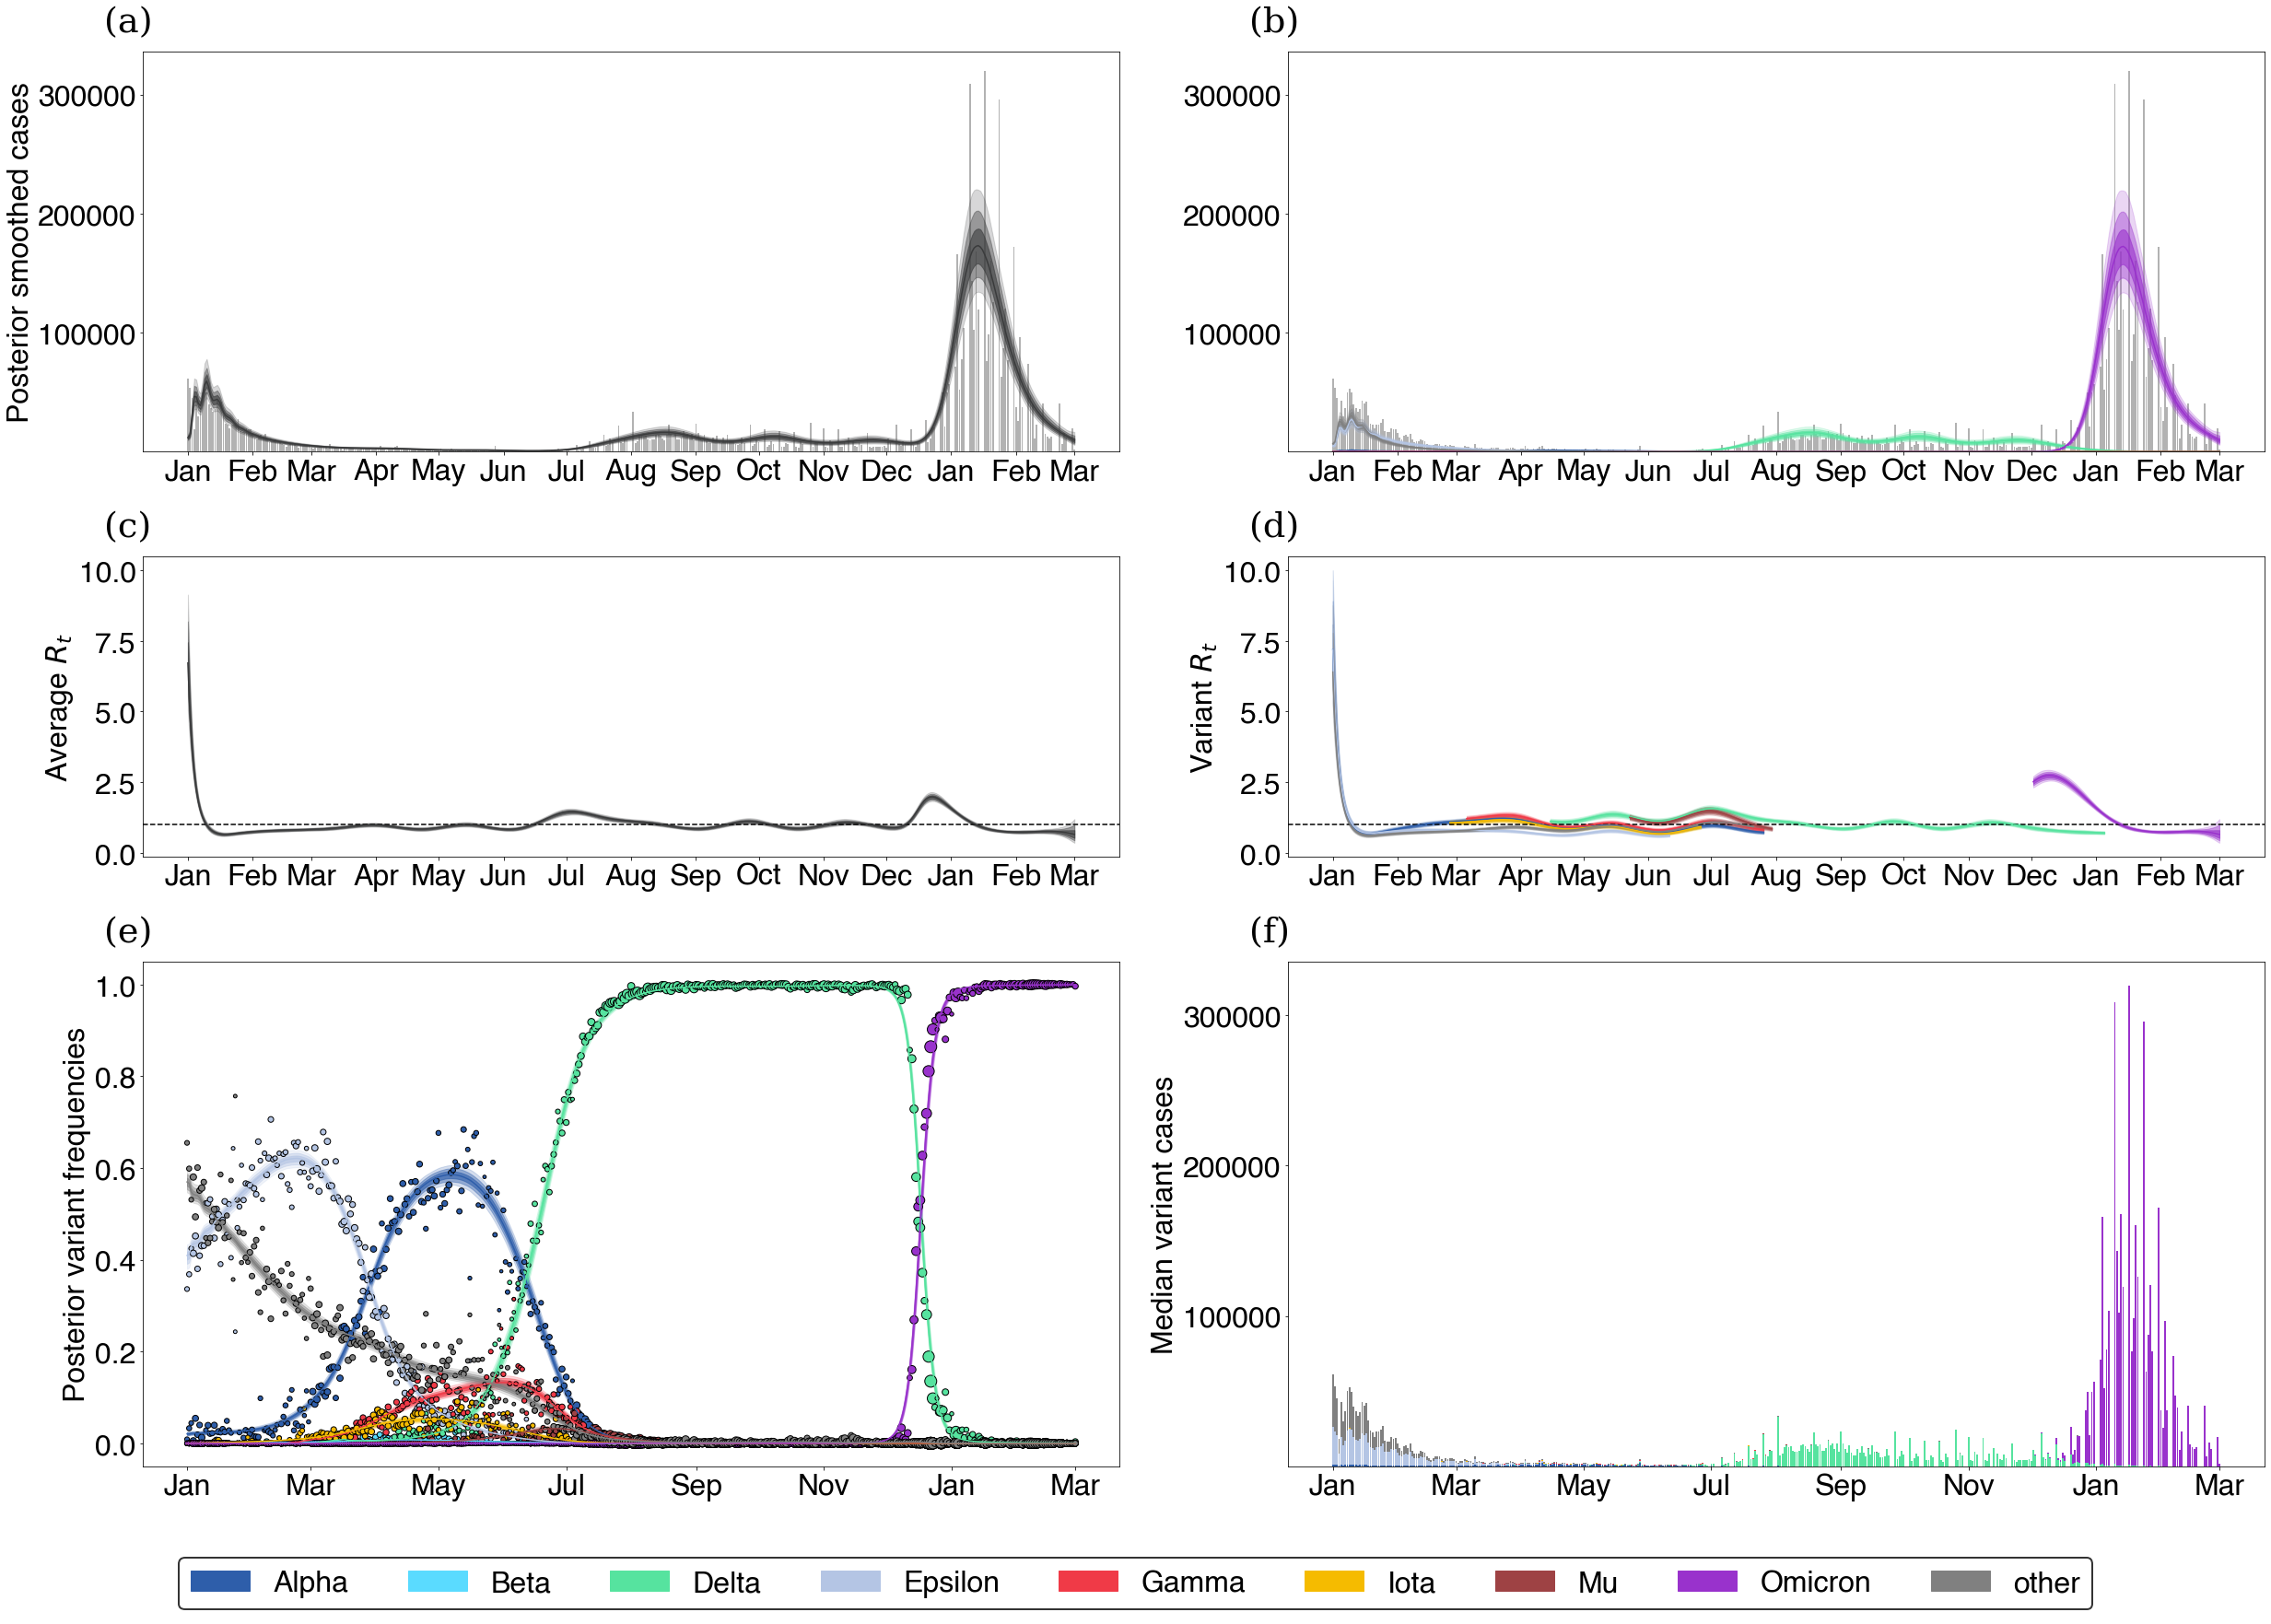
\includegraphics[width=\linewidth]{figs/GARW_rt_California.png}
  \caption{\textbf{Fitting the GARW model to California data.}}%
  \label{fig:GARW_rt_California}
\end{figure}

\begin{figure}
  \centering
  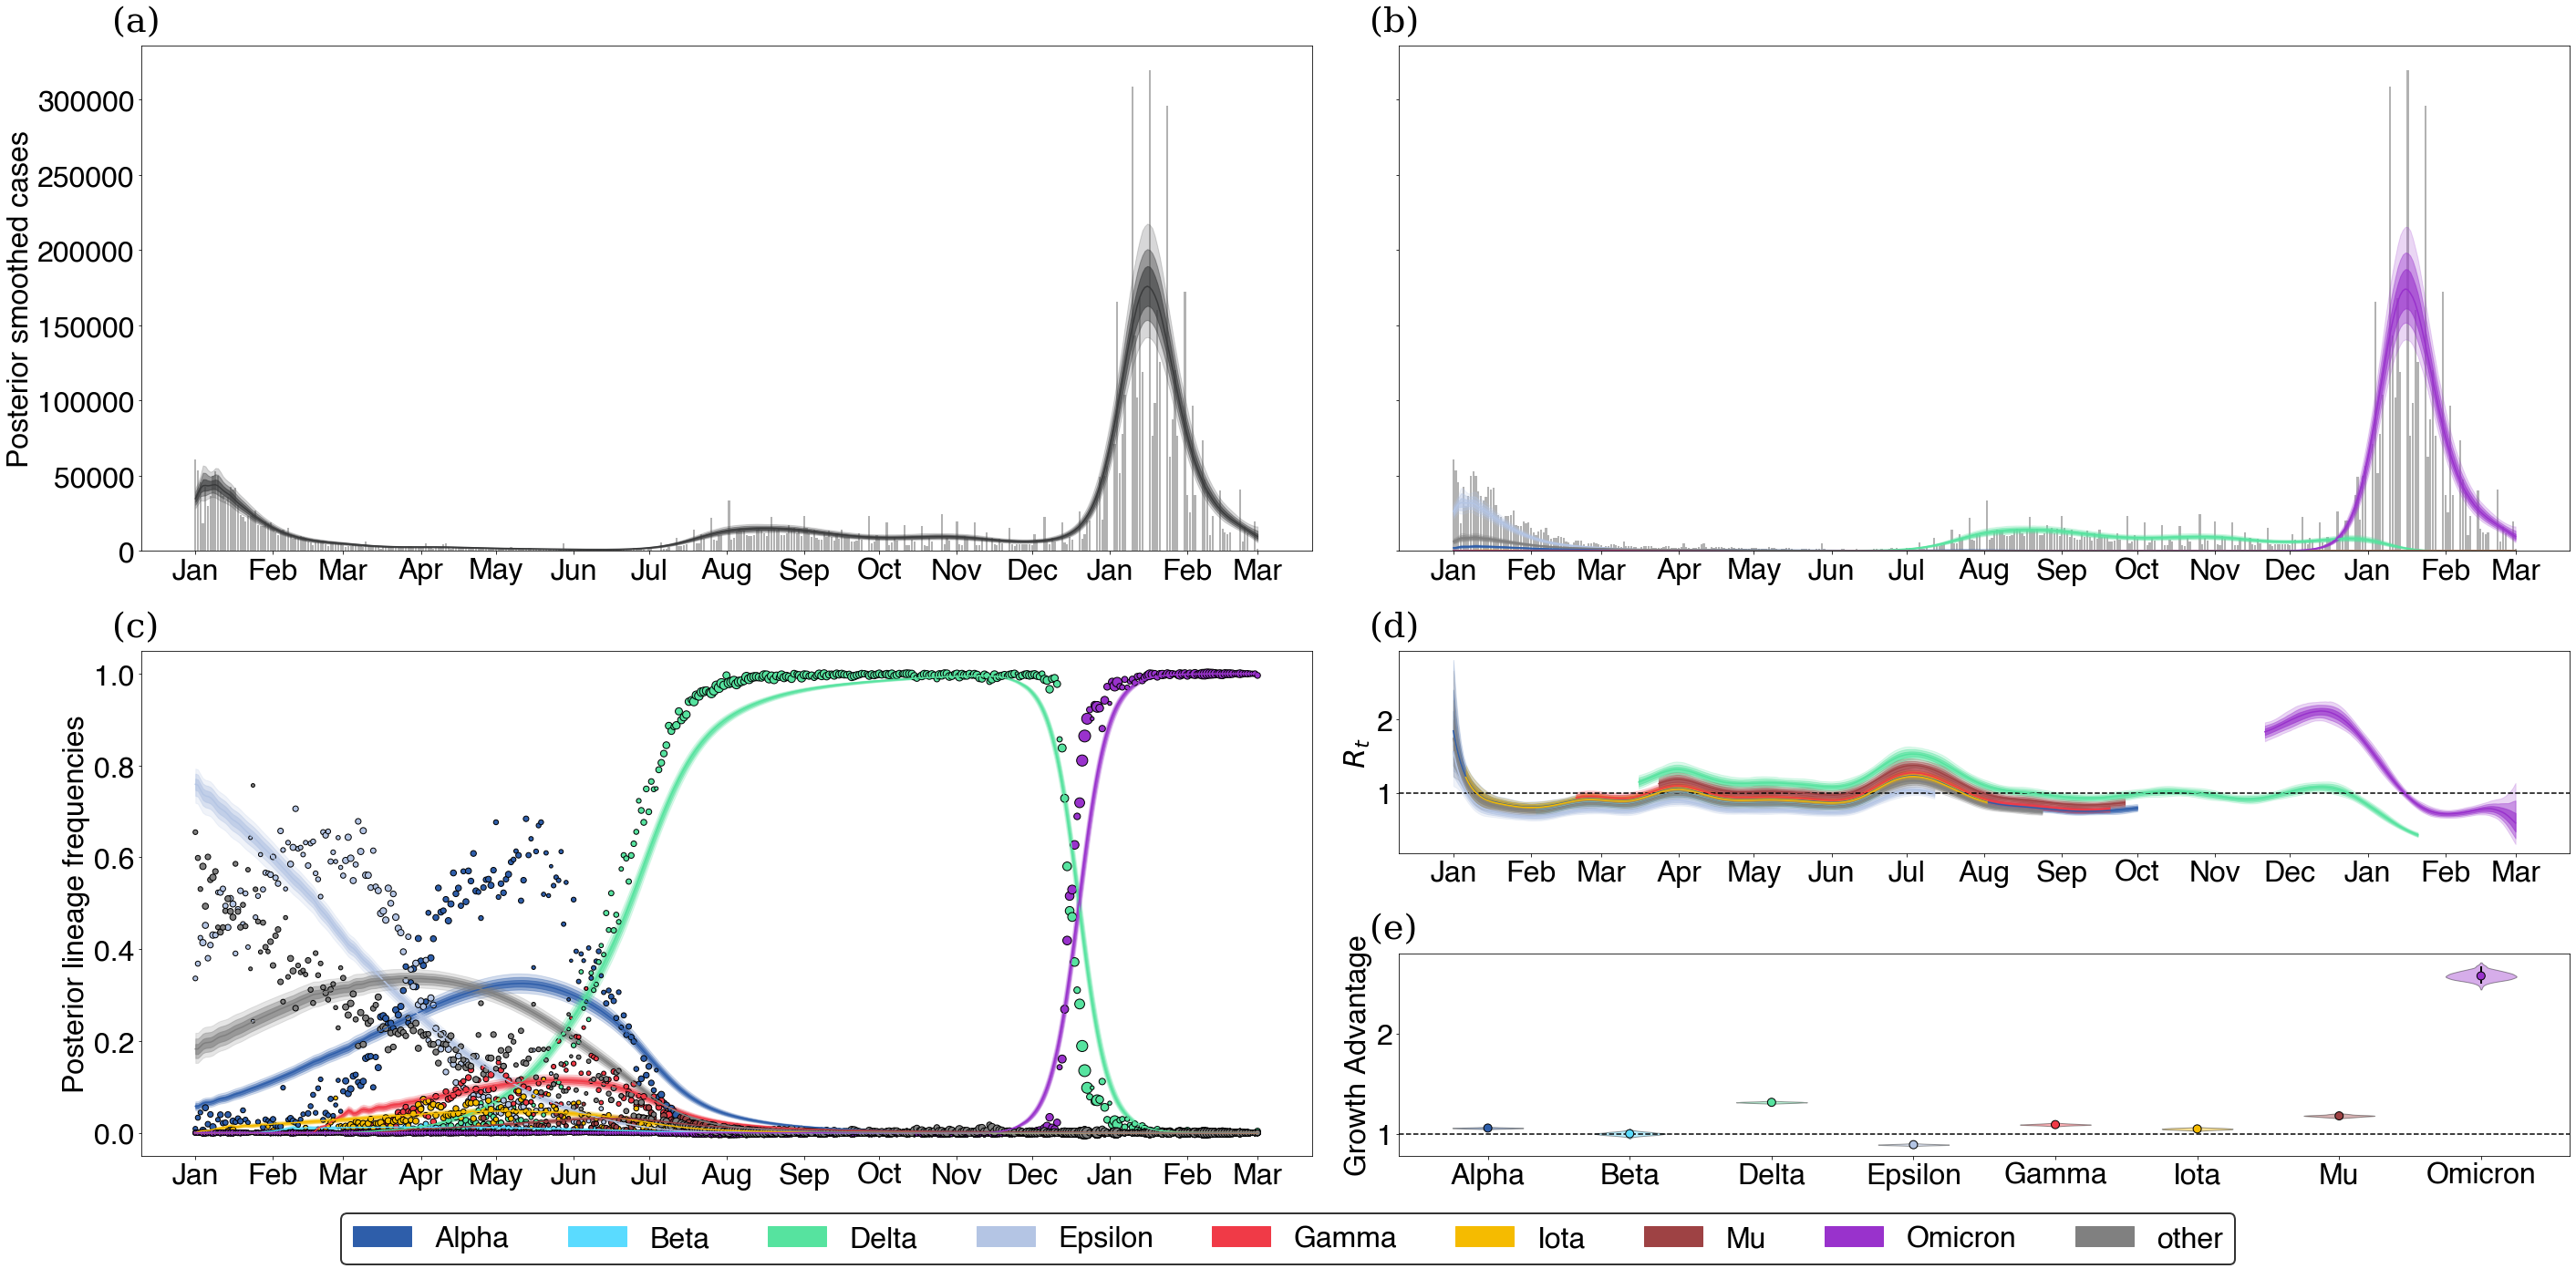
\includegraphics[width=\linewidth]{figs/fixed_growth_California.png}
  \caption{\textbf{Fitting the fixed growth advantage model to California data.}}%
  \label{fig:fixed_growth_California}
\end{figure}

\begin{figure}
  \centering
  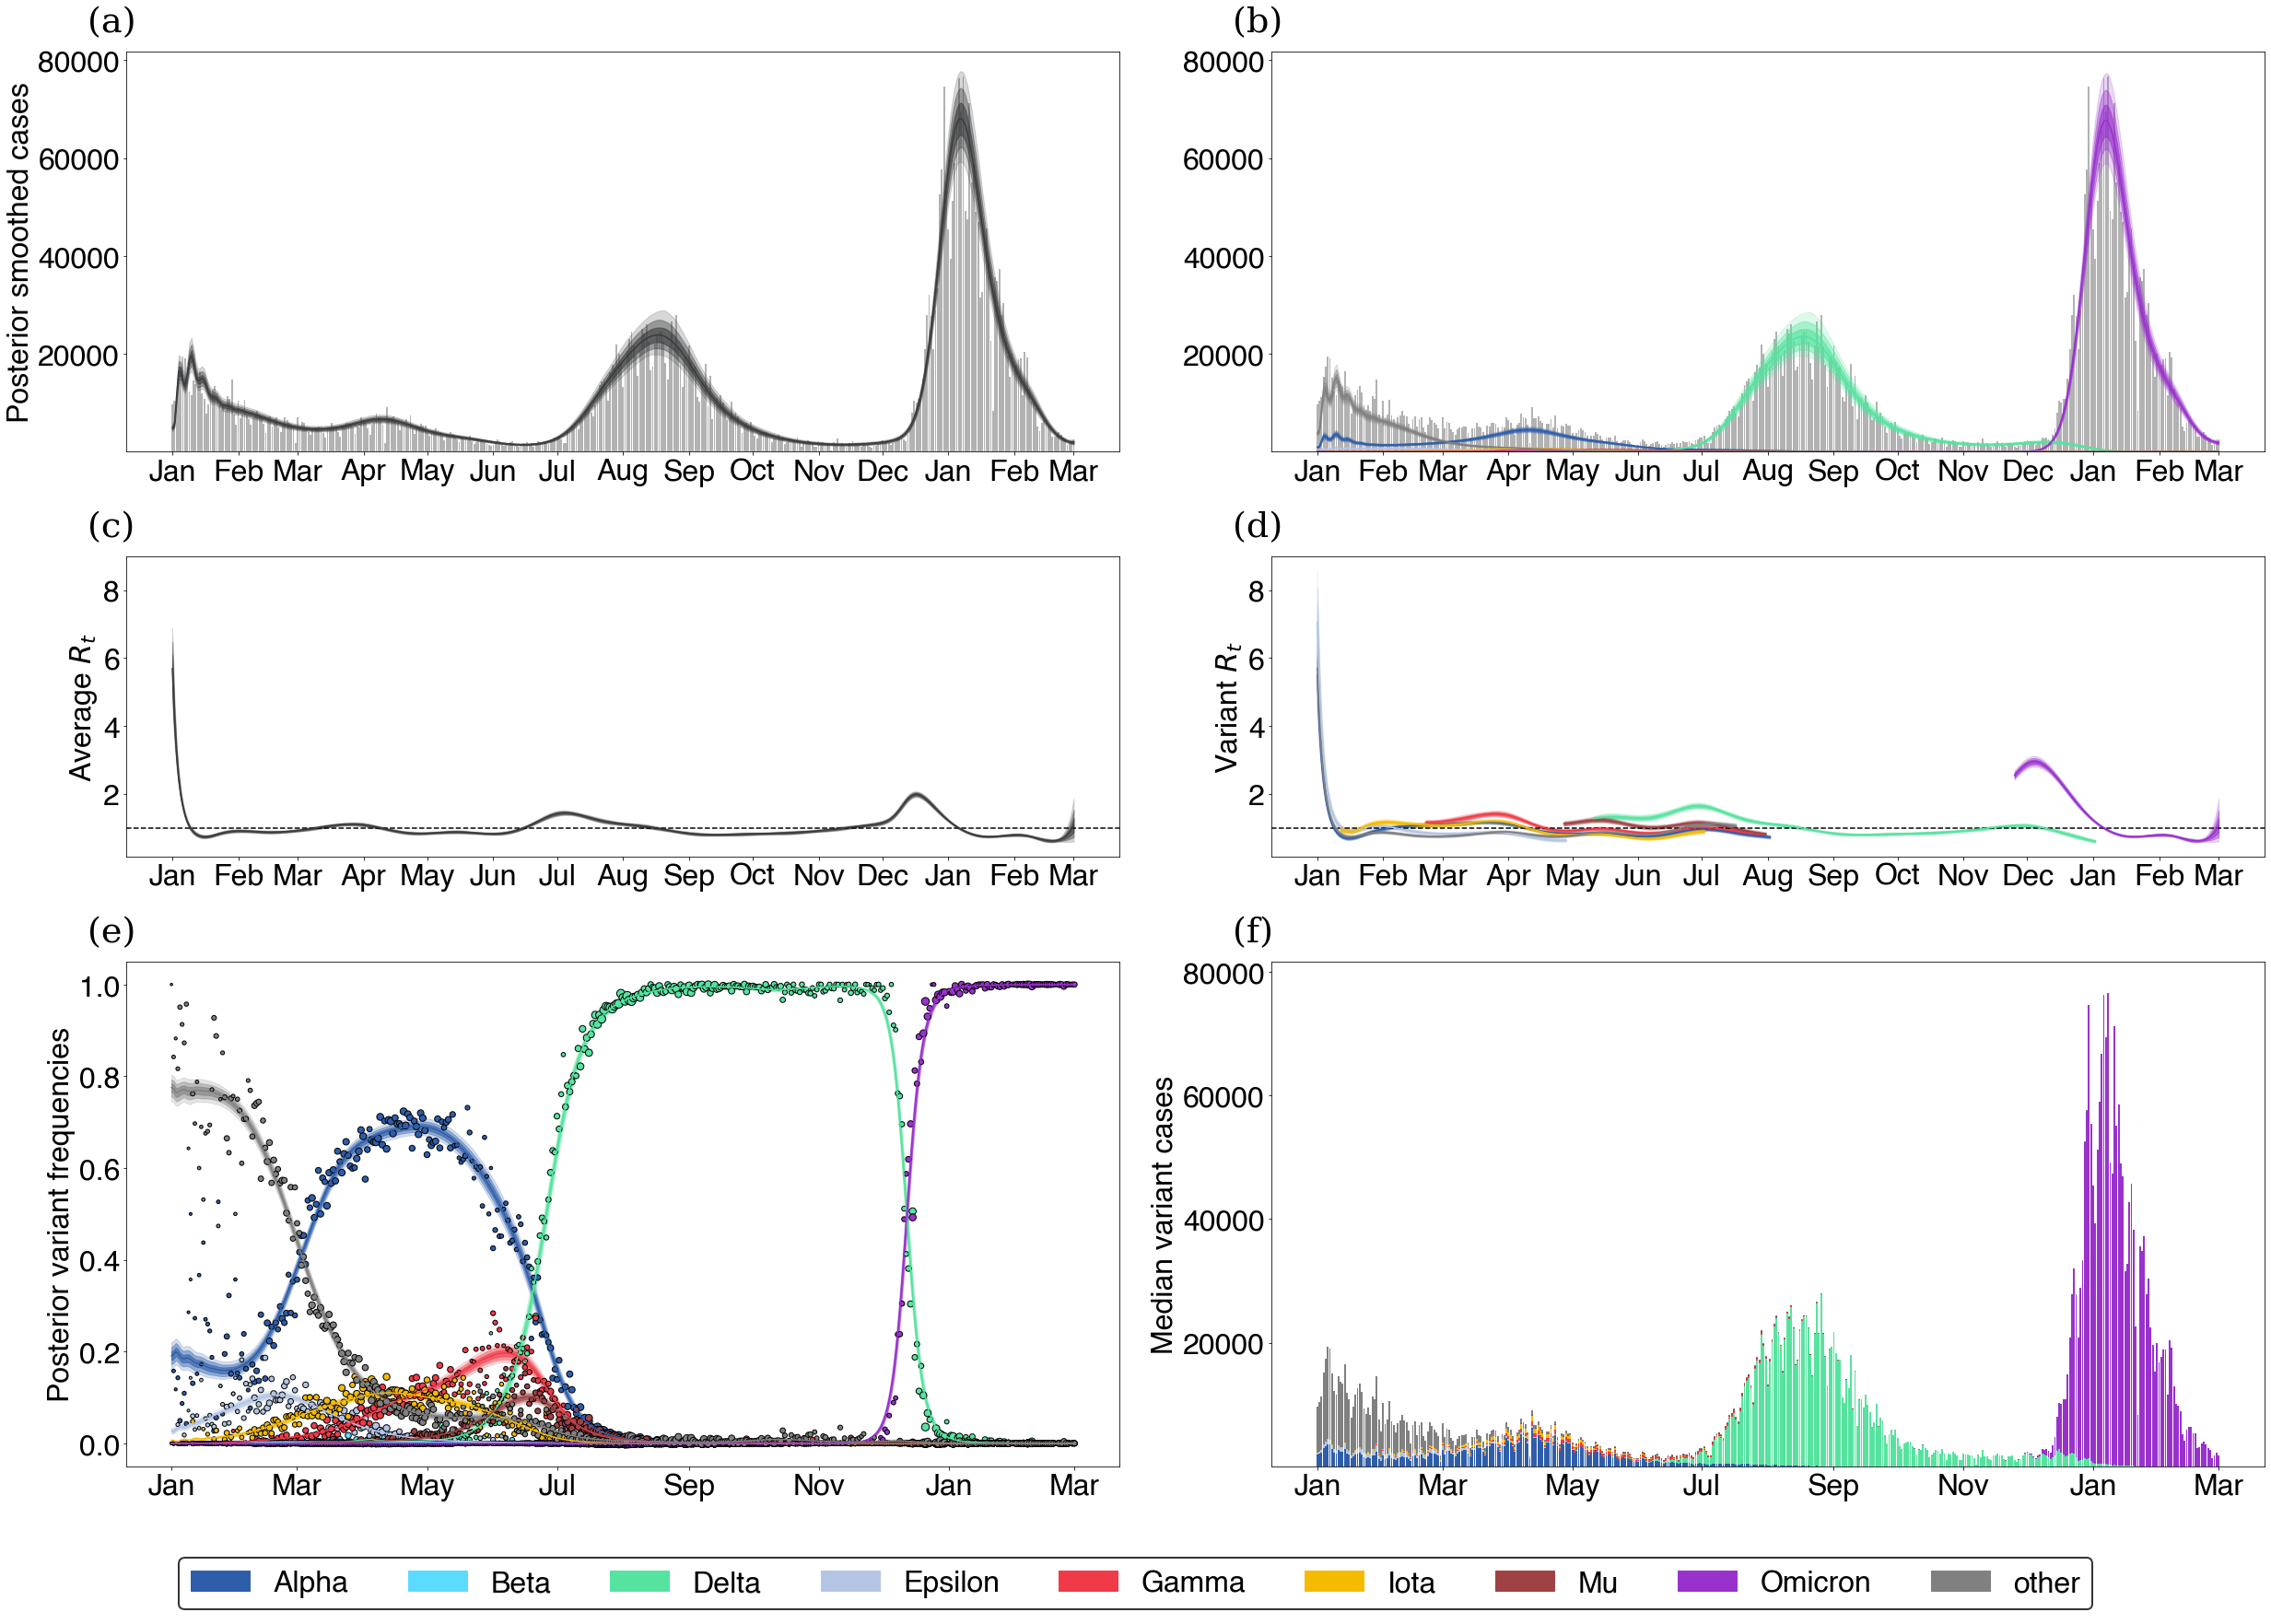
\includegraphics[width=\linewidth]{figs/GARW_rt_Florida.png}
  \caption{\textbf{Fitting the GARW model to Florida data.}}%
  \label{fig:GARW_rt_Florida}
\end{figure}

\begin{figure}
  \centering
  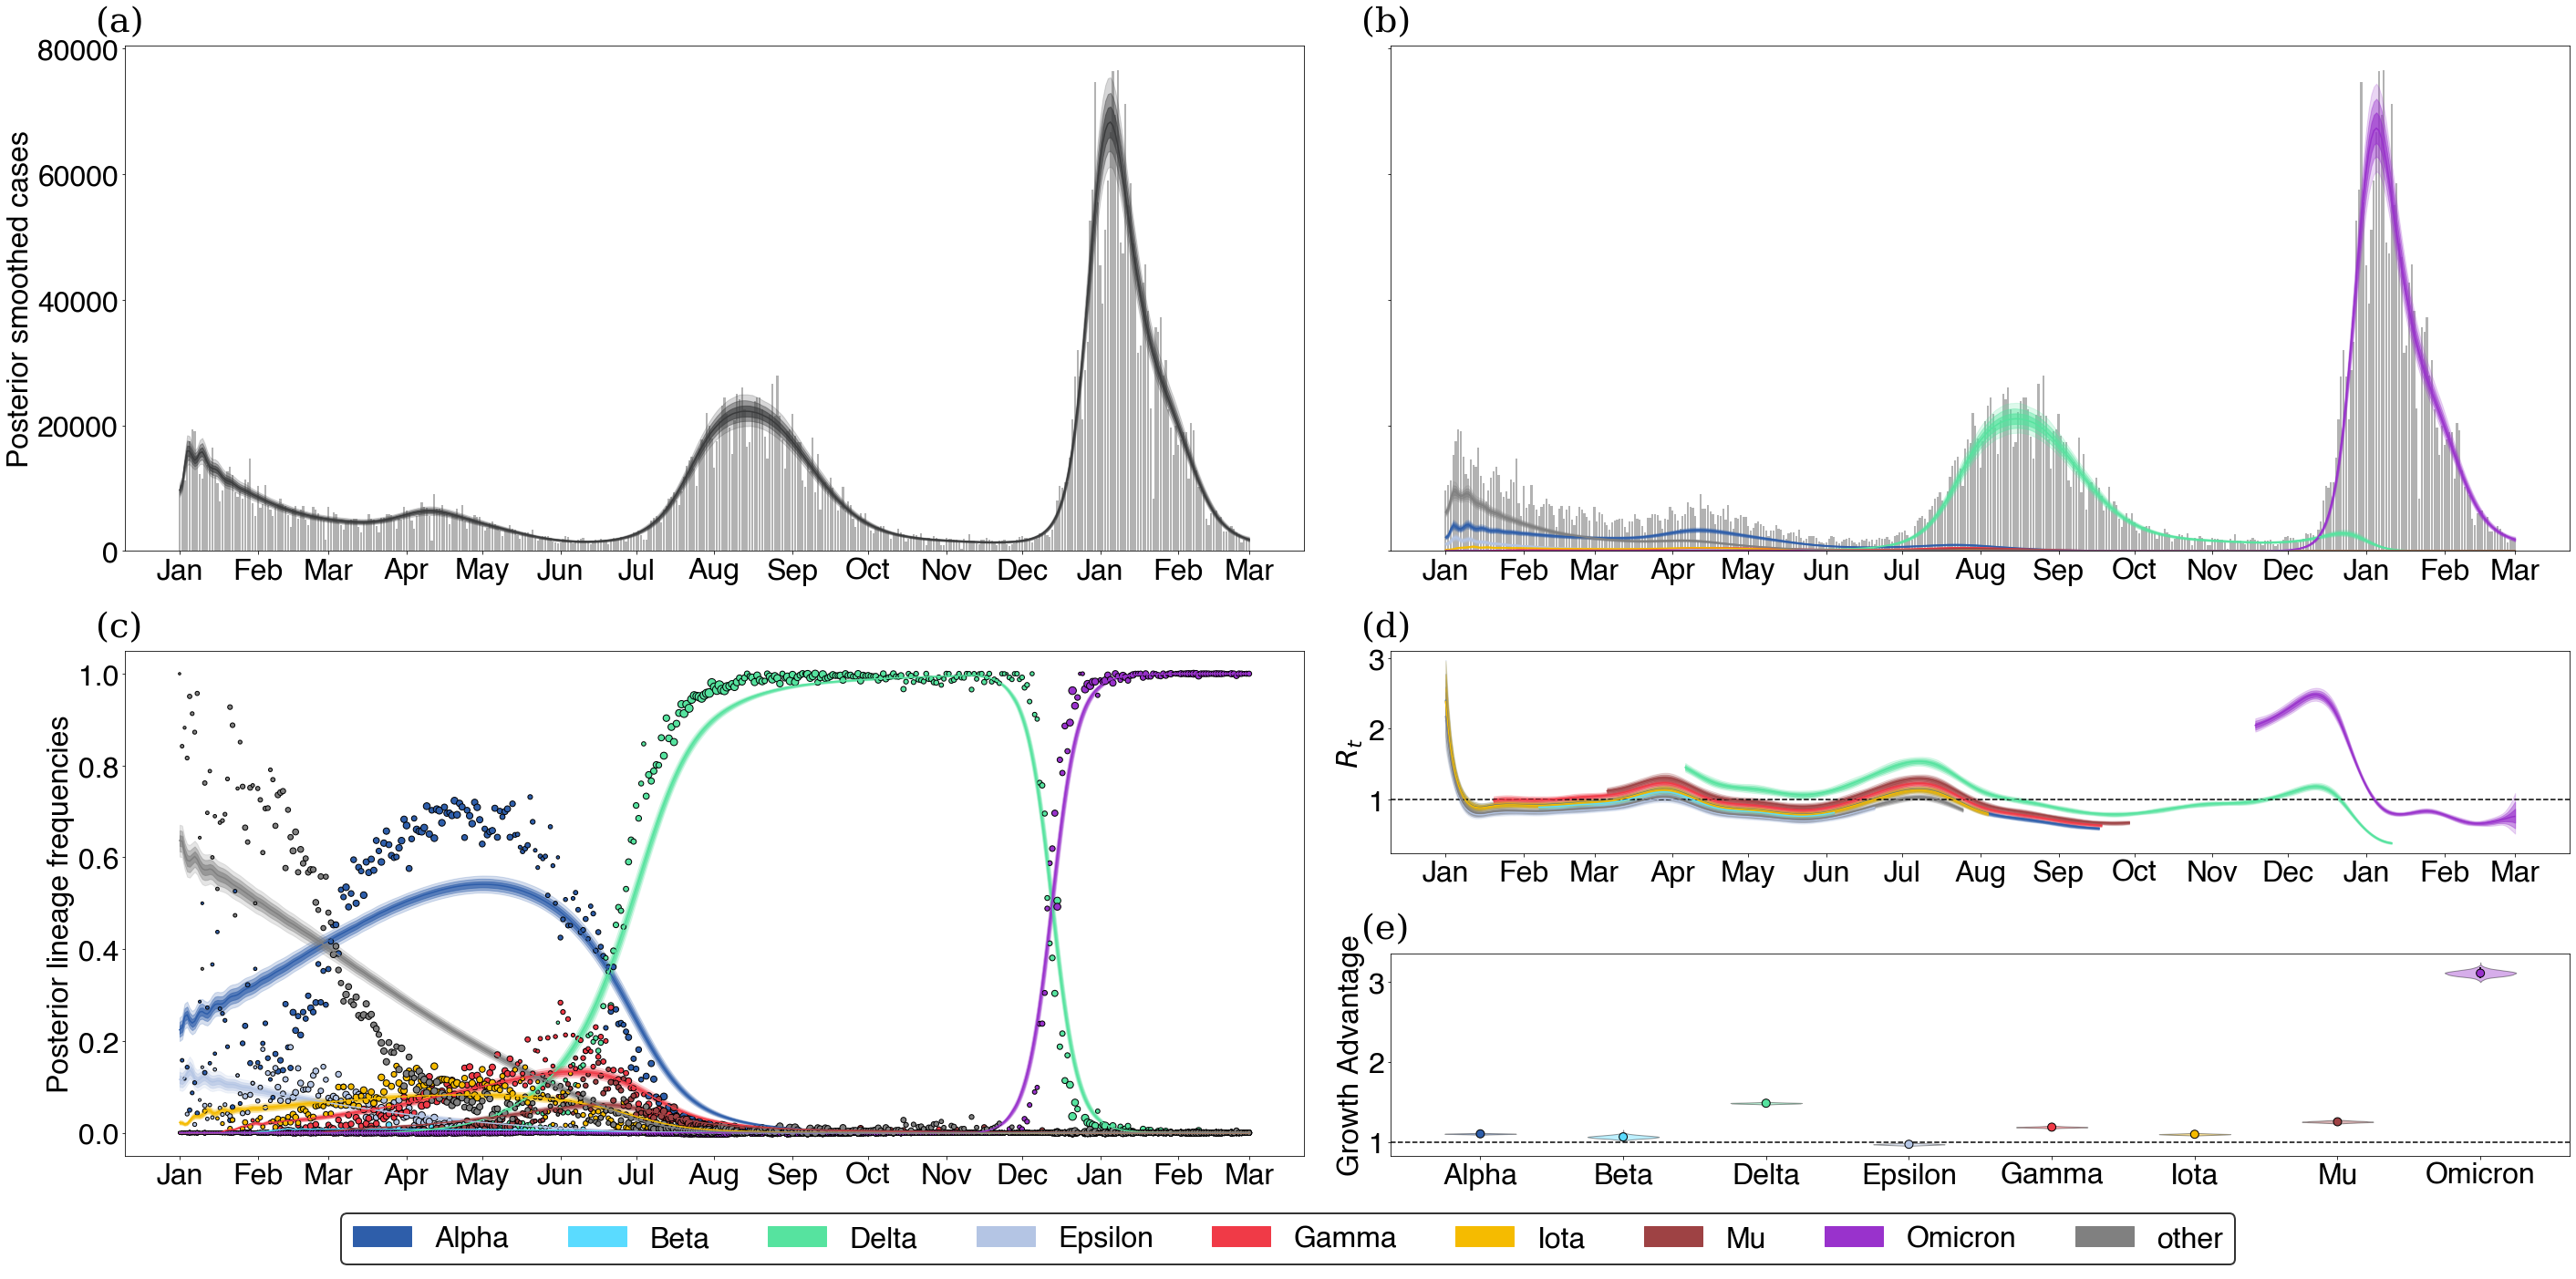
\includegraphics[width=\linewidth]{figs/fixed_growth_Florida.png}
  \caption{\textbf{Fitting the fixed growth advantage model to Florida data.}}%
  \label{fig:fixed_growth_Florida}
\end{figure}

\begin{figure}
  \centering
  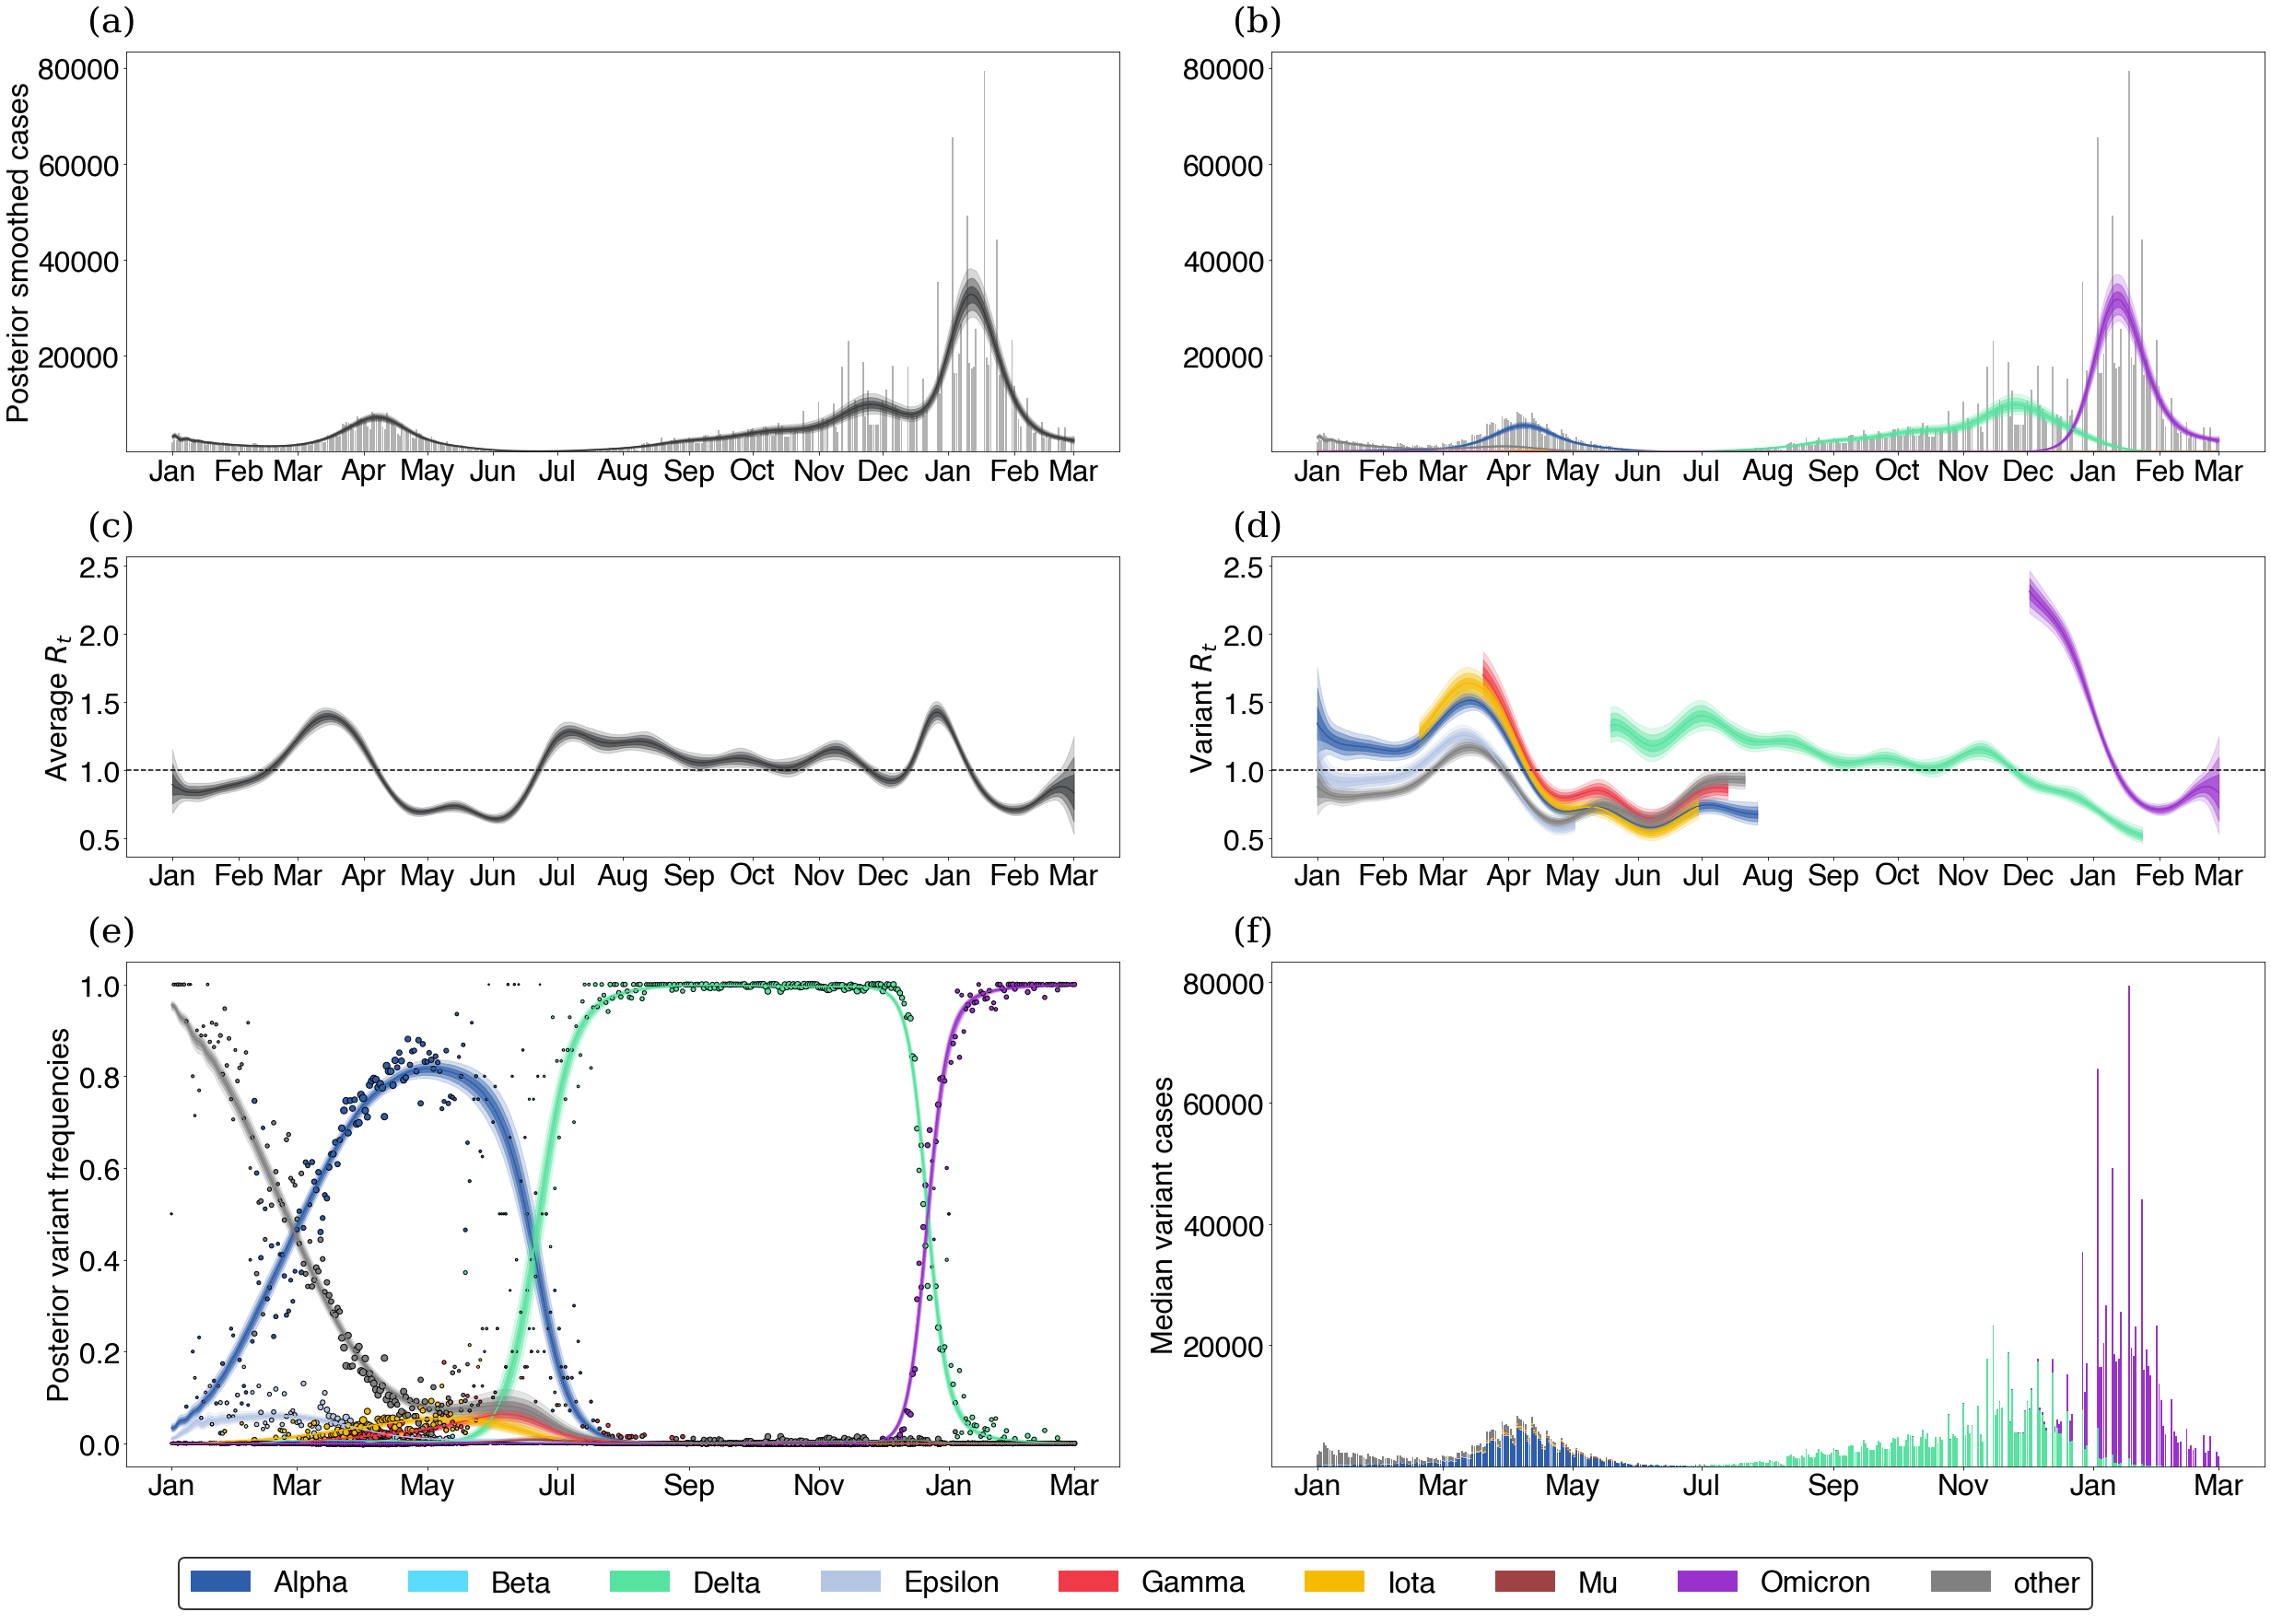
\includegraphics[width=\linewidth]{figs/GARW_rt_Michigan.png}
  \caption{\textbf{Fitting the GARW model to Michigan data.}}%
  \label{fig:GARW_rt_Michigan}
\end{figure}

\begin{figure}
  \centering
  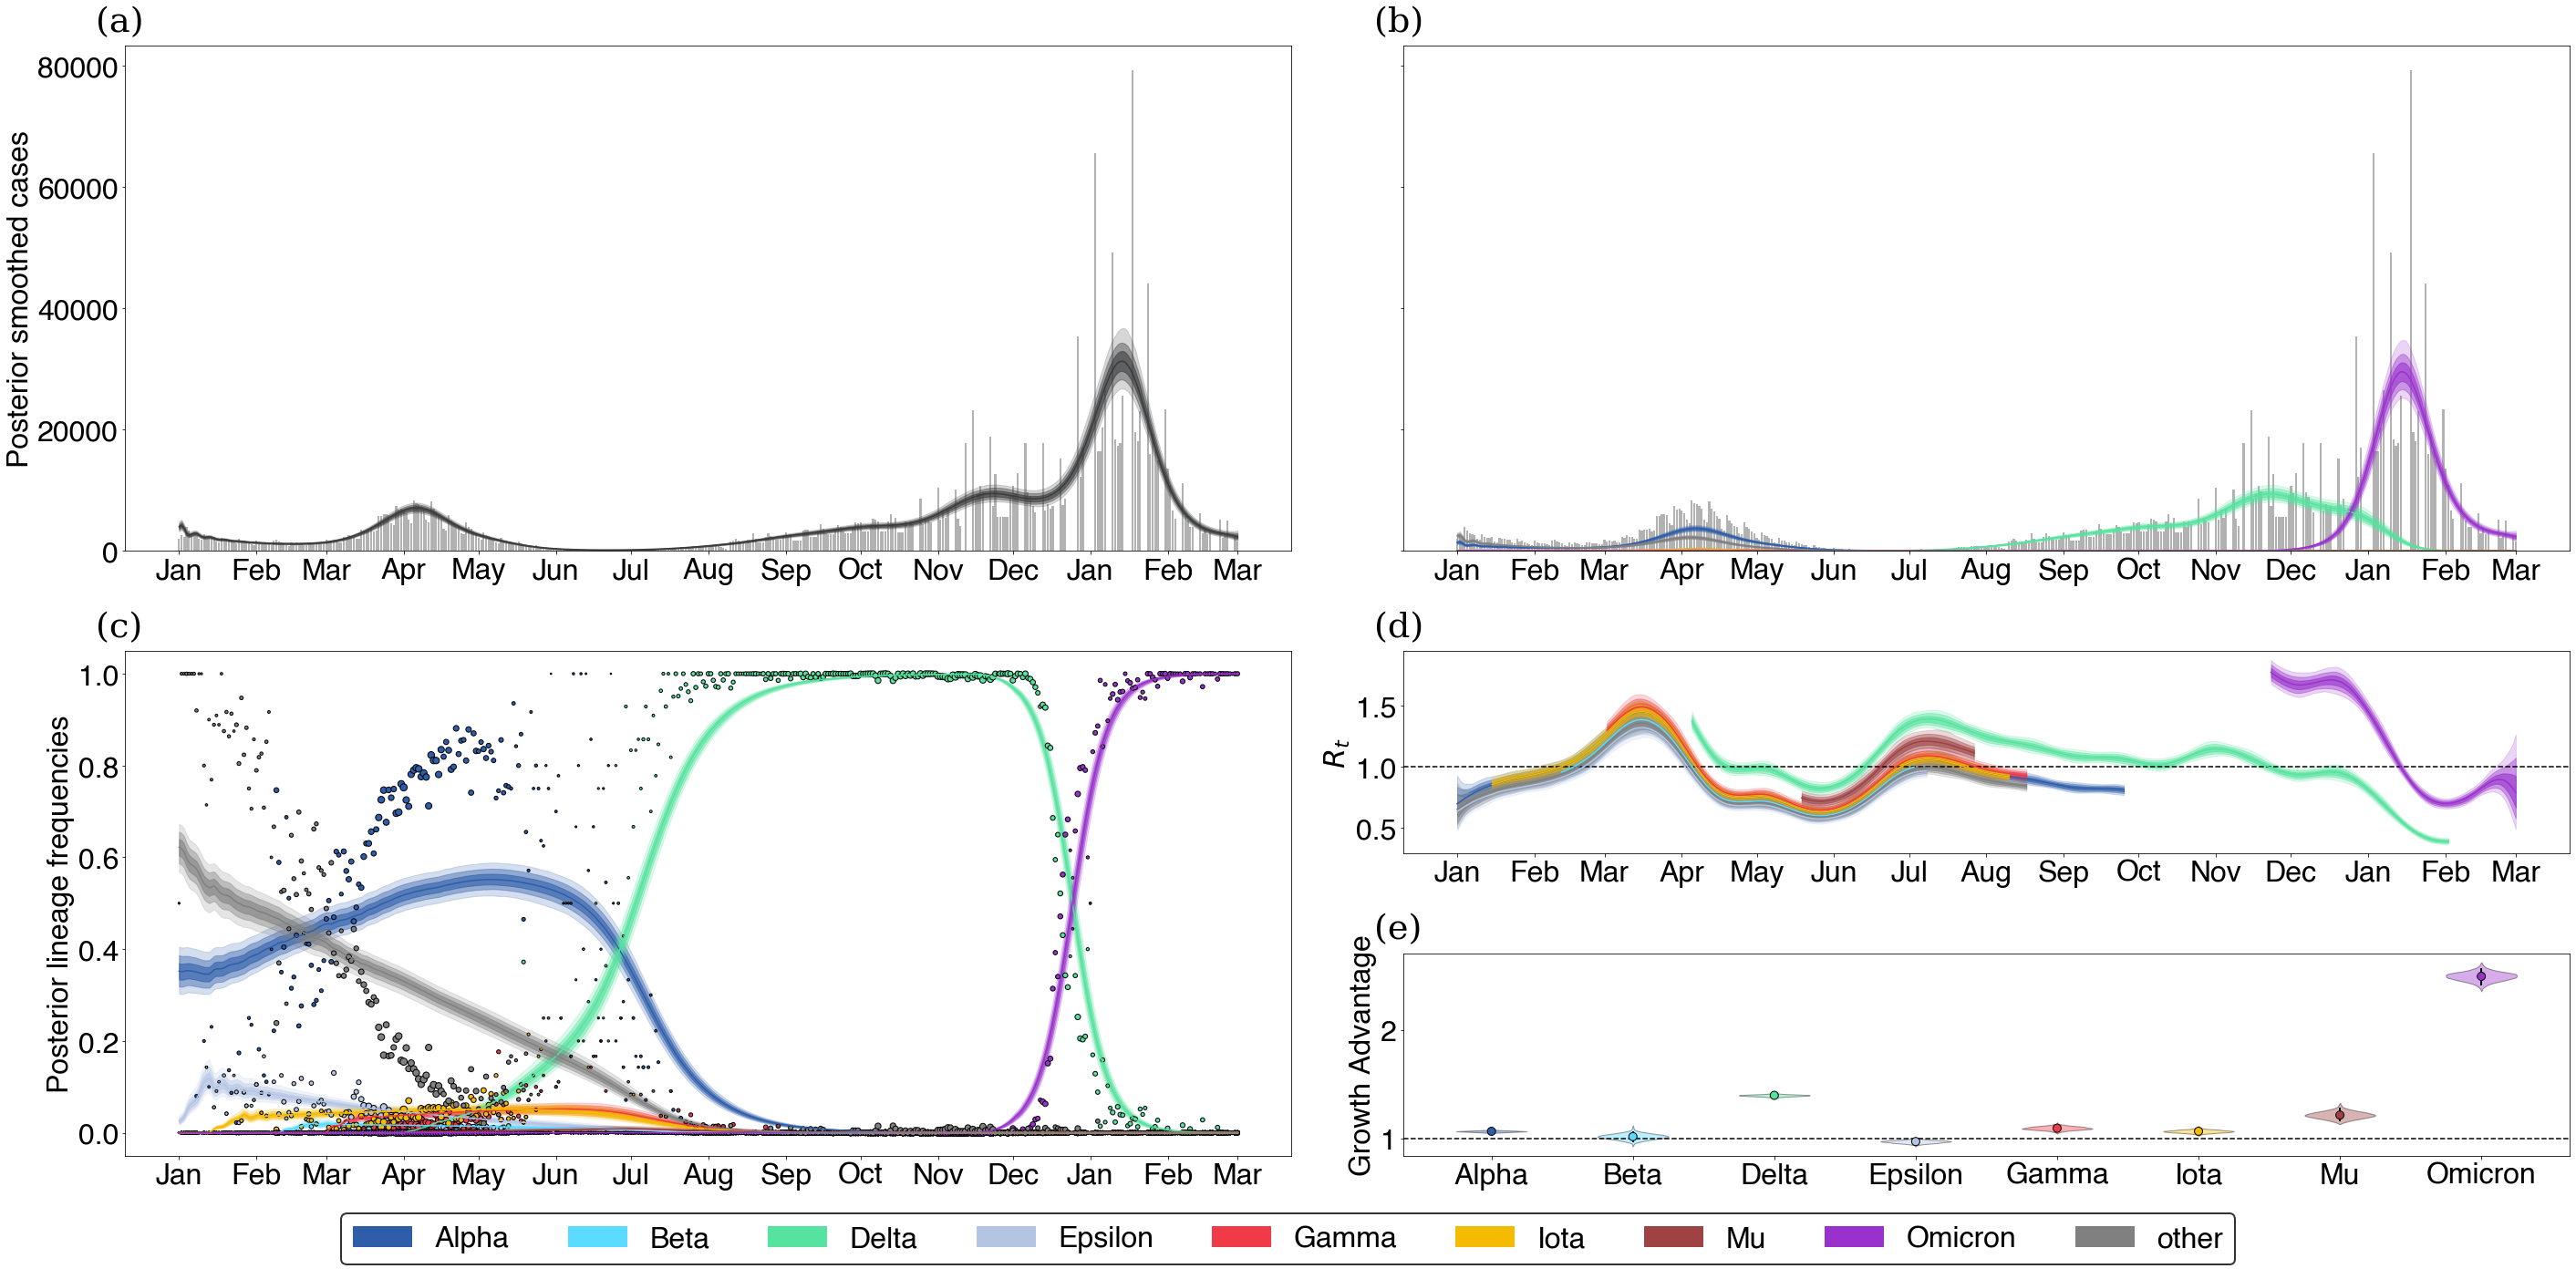
\includegraphics[width=\linewidth]{figs/fixed_growth_Michigan.png}
  \caption{\textbf{Fitting the fixed growth advantage model to Michigan data.}}%
  \label{fig:fixed_growth_Michigan}
\end{figure}

\begin{figure}
  \centering
  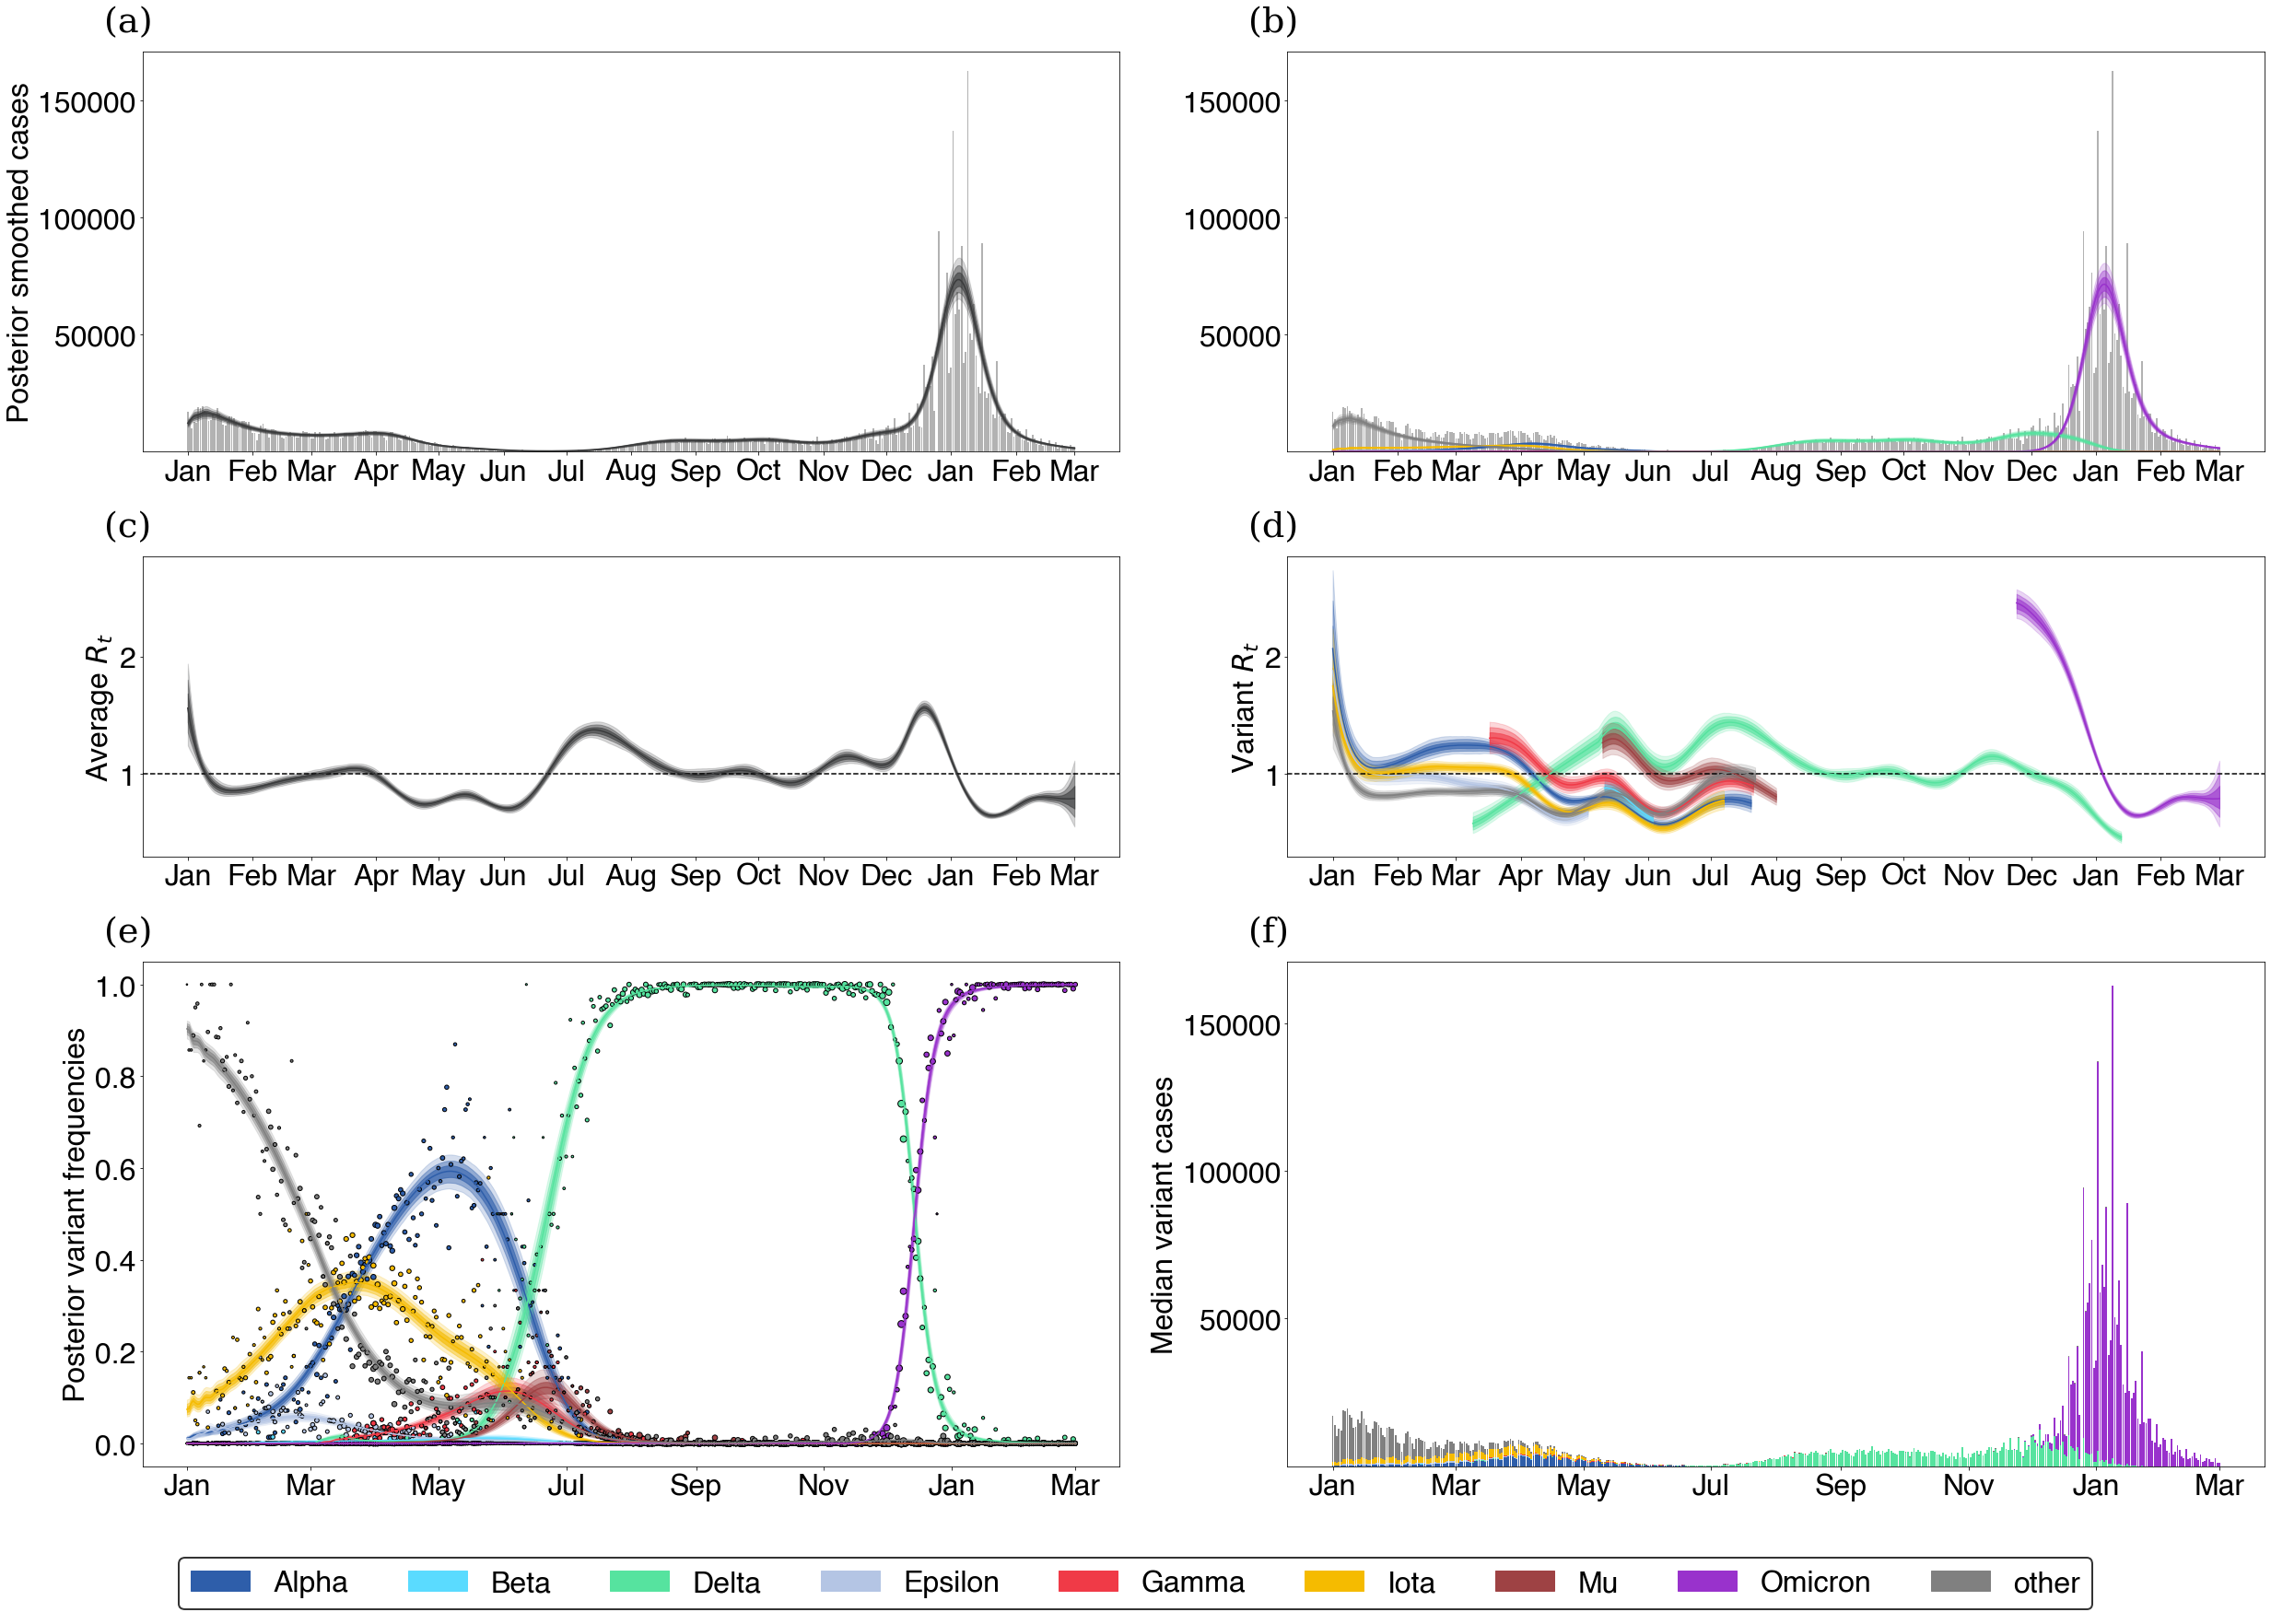
\includegraphics[width=\linewidth]{figs/GARW_rt_New-York.png}
  \caption{\textbf{Fitting the GARW model to New York state data.}}%
  \label{fig:GARW_rt_New-York}
\end{figure}

\begin{figure}
  \centering
  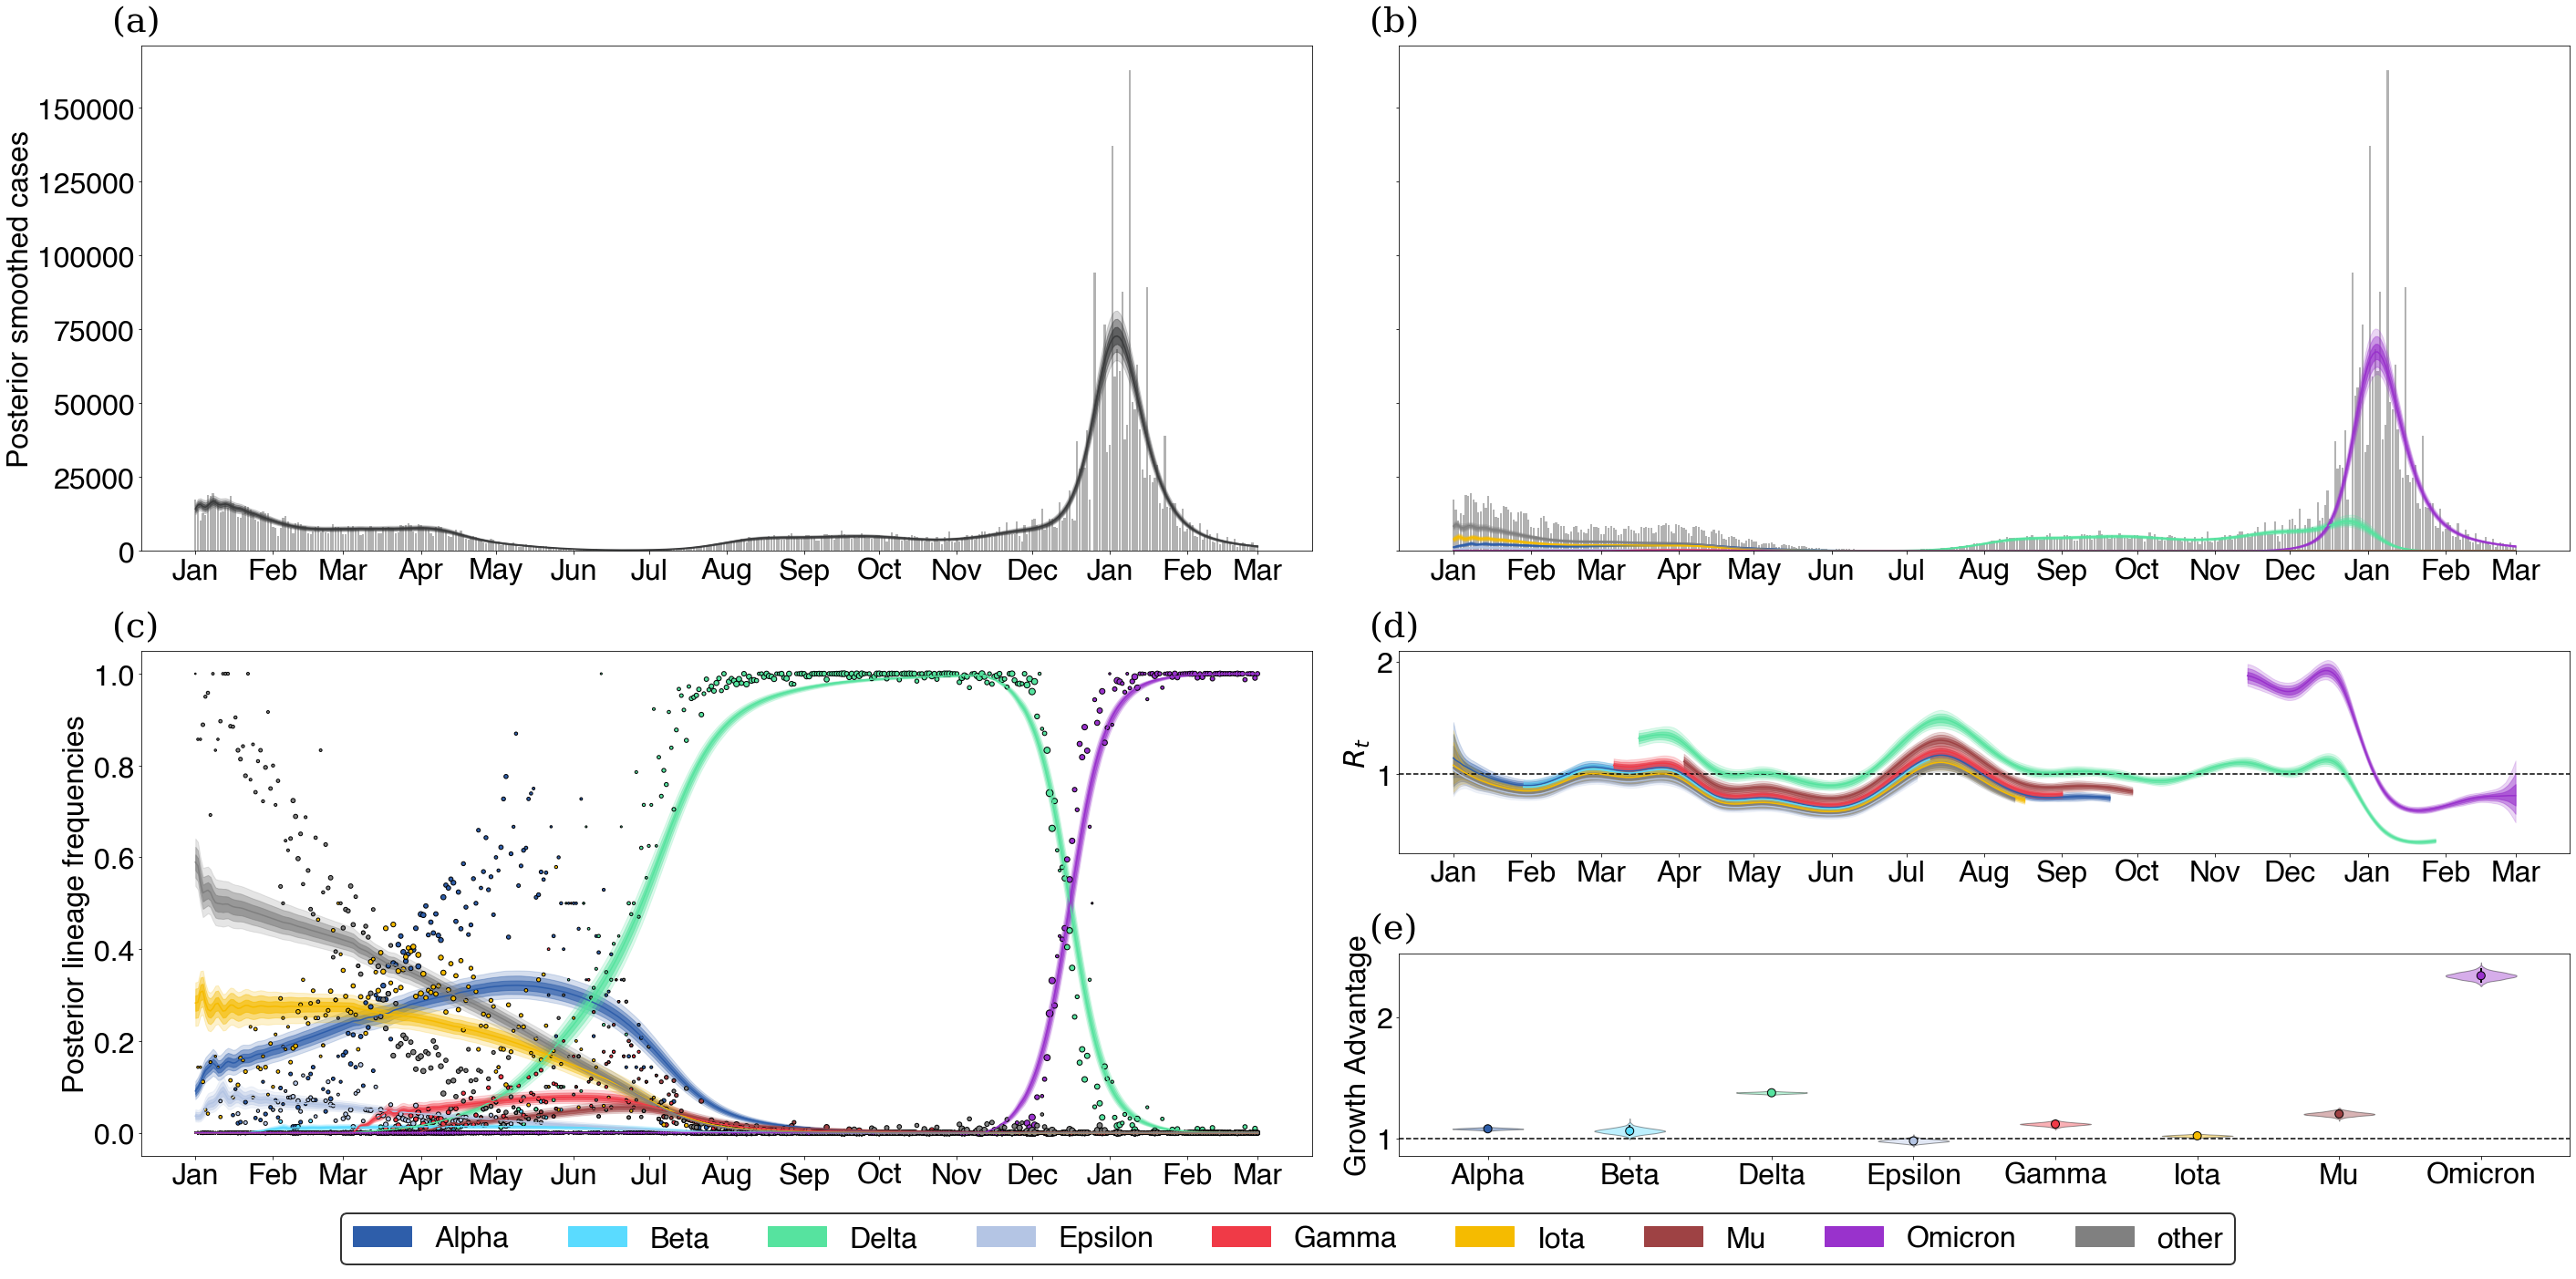
\includegraphics[width=\linewidth]{figs/fixed_growth_New-York.png}
  \caption{\textbf{Fitting the fixed growth advantage model to New York state data.}}%
  \label{fig:fixed_growth_New-York}
\end{figure}

\clearpage


\graphicspath{{./chapters/rt-from-frequency-dynamics/}}
\chapter{Supplementary Materials for Chapter 2} 

%TODO: Make sure we use supplementary results -> supplementary figures

\section{Supplementary Text}

\subsection*{Relationship to multinomial logistic regression}

Other papers have tried to infer growth advantages of variants from sequence data alone, we show that the multinomial logistic regression model typically used in these analysis is roughly equivalent to our fixed growth advantage model, but that inferring relative effective reproduction numbers between variants using multinomial logistic regression requires additional restrictions on the generation time.
Multinomial logistic regression typically models the probability of a given observation belong to class $v$ at time $t$ as
\begin{equation}
  f_{v}(t) = \frac{p_{v}\exp(\beta_{v} t)}{\sum_{1\leq u\leq V} p_{u}\exp(\beta_{u} t)}.
\end{equation}
For our purpose, we can assume this probability is equivalent to the true frequency of variant $v$ in the population and in this case, $p_{v}$ is considered to be related to the prevalence on variant $v$ in the population at $t=0$ and $\beta_{v}$ can be considered to be the growth advantage relative to a pivot class $u_{*}$ which has $\beta_{k_{*}} = 0$.
In order to see the connection between the above model and ours, we return to the original renewal equation of the form
\begin{equation}
  I(t) = R_{t}\int_{0}^{t} I(t-\tau) g(\tau).
\end{equation}
Assuming that $g$  is a point mass at a mean generation time $T_{g}$, we have that
\begin{equation}
  I(nT_{g}) = \left(\prod_{i=1}^{n} R_{iT_{g}}\right) I(0).
\end{equation}
Assuming that there are several variants following these same dynamics, we have that the frequency of a given variant $v$ can be written as
\begin{equation}
  f_{v}(nT_{g}) = \frac{I_{v}(nT_{g})}{\sum_{1\leq u \leq V} I_{u}(nT_{g})}.
\end{equation}
If we assume a constant growth advantage as in our model, we then have that $R_{t,v} = \Delta_{v} R_{t}$, so that
\begin{equation}
  f_{v}(nT_{g}) =  \frac{\Delta_{v}^{n} I_{v}(0)}{\sum_{1\leq u \leq V} \Delta_{u}^{n} I_{u}(0)}.
\end{equation}
Writing $\Delta_{v} = \exp(\delta_{v})$ and $t = n T_{g}$, allows us to see that
\begin{equation}
  f_{v}(t) = \frac{I_{v}(0) \exp(\frac{\delta_{v}}{T_{g}} t)}{\sum_{1\leq u \leq V}I_{u}(0) \exp(\frac{\delta_{u}}{T_{g}} t)}.
\end{equation}
By fixing one pivot class so that $I_{u_{*}} = 1$ and $\delta_{u_{*}} / T_{g} = 0$, we can identify our model with the multinomial logistic regression by relating the parameters as

\begin{align}
  \delta_{v} &= \beta_{v}T_{g}\\
  I_{v}(0) &= p_{v}.
\end{align}

This shows that the multinomial logistic regression functions similarly to our fixed growth advantage model except with the additional assumption that the generation time is a point mass at $T_{g}$.
This assumption additionally allows us to relate the epidemic growth rate $r$ and the effective reproduction number as $R = \exp(r T_{g})$ \cite{Wallinga2006}.
Therefore, by further assuming that the variant infections are exponentially growing with rates $r_{v}$, we can then identify $\beta_{v} = r_{v} - r_{u_{*}}$.
This means that the relative effective reproduction number for any two variants can be written as
\begin{align*}
\ln \left( \frac{R_{t,v}}{R_{t,u}} \right) = (\beta_{v} - \beta_{u}) T_{g}.
\end{align*}

\begin{figure}
  \centering
  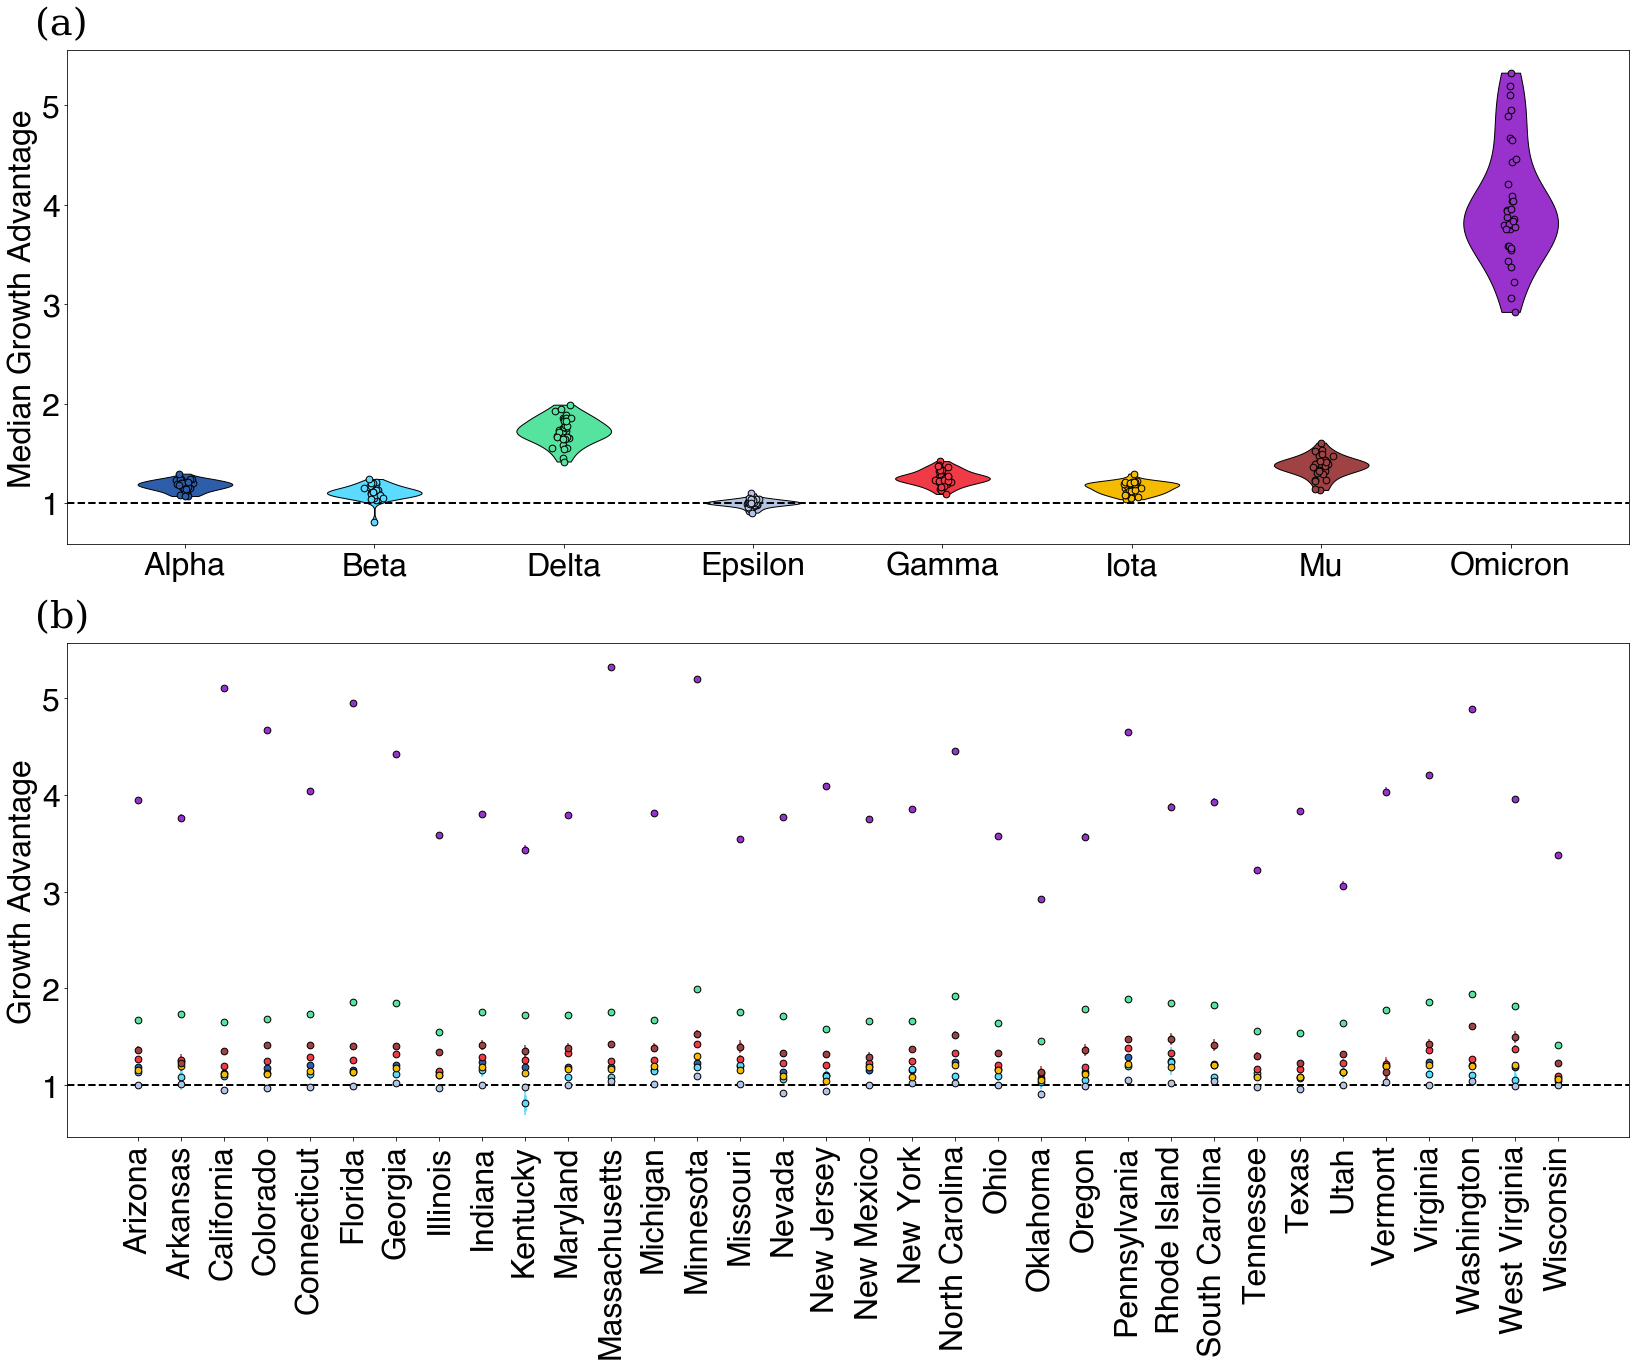
\includegraphics[width=\linewidth]{figs/fig_MLR_growth_advantages_supp.png}
  \caption{Estimating variant growth advantages in various states using Multinomial Logistic Regression model assuming generation time $T_{g} = 5.2$.
  (a) Growth advantages visualized by state.
  (b) Same as (a) but grouped by variant.}%
  \label{fig:MLR_growth_advantages}
\end{figure}

\newpage

\subsection*{Relating epidemic growth rates to relative effective reproduction numbers}

An important relationship of interest is between the epidemic growth rate of an epidemic and its effective reproduction number.
In the case of our analysis, we are particularly interested in the effect of generation time assumptions on estimated variant-specific effective reproduction numbers.
First, notice that the effective reproduction number and the epidemic growth rate of an epidemic are related by
\begin{align*}
R_{t} = \frac{1}{\int_{0}^{\infty} \exp(-r\tau)g(\tau)d\tau} = \frac{1}{M_{g}(-r)}
\end{align*}
according to the Lotka-Euler equation \cite{Wallinga2006} where $r$ is the epidemic growth rate and $M_{g}$ is the moment-generating function of the generation time $g$.

This allows us to write the relative reproduction number of two variants $v$ and $u$ as a function of their epidemic growth rates, so that
\begin{align*}
\frac{R_{t,v}}{R_{t,u}} = \frac{M_{g}(-r_{u})}{M_{g}(-r_{v})}.
\end{align*}

We'll consider three common generation time assumptions. First, we consider the case where the generation time is a point mass at $T_{g}$. In which case, $M_{g}(-r) = \exp(-r T_{g})$ and we recover the relationship
\begin{align*}
R_{t,v} = \exp(r_{v}T_{g}).
\end{align*}

In this case, the relative effective reproduction number will depend on only the difference between the epidemic growth rates and therefore, is commonly used when converting estimated growth advantages to relative reproduction numbers in the case of logistic growth models.

Second, we consider the case where the generation time is an exponential distribution with mean $T_{g}$. This assumption is often implicit and common in models of infectious diseases such as ODEs and their stochastic variants. Using the corresponding moment-generating function, we see that
\begin{align*}
R_{t,v} = 1 + r_{v} T_{g}
\end{align*}

Next, we consider the Gamma distributed generation times with mean $T_{g}$ and standard deviation $s$.
This is often used in models of infectious diseases via the chain trick in which multiple compartments are chained together to obtain non-exponential generation times or infectious periods.
Re-parameterizing the Gamma distribution in terms of its mean and standard deviation and using its moment generating function, we have that
\begin{align*}
R_{t,v} = \left(1 + r_{v}  \left(\frac{s^{2}}{T_{g}}\right) \right)^{T_{g}^{2} / s^{2}}.
\end{align*}

From this equation, we can see that increases in the mean of the generation time of $v$ leads to decreasing estimates of $R_{t,v}$ during epidemic decline ($r_{v} < 0$) and increased estimates during epidemic growth ($r_{v} > 0$) assuming $r_{v}$ and $s$ are fixed.
Additionally, increases in the standard deviation will generally lead to lower inferred variant advantages.
This effect is also visualized in Figure \ref{fig:generation_time_sensitivity}.

\paragraph{Variant growth-advantages are sensitive to generation time}%

In the case where we have two variants $u, v$ with Gamma-distributed generation times with means $T_{u}, T_{v}$ and standard deviations $s_{u}, s_{v}$ respectively, we can then write the relative effective reproduction number of $v$ over $u$ as
\begin{align*}
\frac{R_{t,v}}{R_{t,u}} = \frac{\left[1 + r_{v}  \left(\frac{s_{v}^{2}}{T_{v}}\right)\right]^{T_{v}^{2} / s_{v}^{2}}}{\left[1 + r_{u} \left(\frac{s_{u}^{2}}{T_{u}}\right)\right]^{T_{u}^{2} / s_{u}^{2}}}.
\end{align*}
It follows that increases in the mean of the generation time of $v$ leads to decreasing inferred variant advantages during epidemic decline and increased advantages during epidemic growth when all quantities are fixed.
On the other hand, increases in the standard deviation will generally lead to lower inferred variant advantages.

Taking a logarithm, we can also evaluate the sensitivity of our inferred growth advantages from our fixed growth advantage model with respect to the generation time assuming it is Gamma distributed as
\begin{align*}
 \delta_{v}  = \ln \left( \frac{R_{t,v}}{R_{t,0}} \right) = \left( \frac{T_{g}^{2}}{s^{2}} \right)  \ln \left( \frac{1 + r_{v}  \left(\frac{s^{2}}{T_{g}}\right)}{1 + r_{0} \left(\frac{s^{2}}{T_{g}}\right) } \right).
\end{align*}
As the log of the relative effective reproduction number, the behavior here is analogous to that discussed above when the mean $T_{g}$ and standard deviation $s$ are changed.
This effects of varying mean and standard deviation are illustrated in Figure \ref{fig:growth_advantage_sensitivity}.
Although the effective reproduction number and the growth advantage appear to have strong dependence on generation time parameters, we find that the epidemic growth rate $r$ is more robust to changes in generation time (see Figure \ref{fig:little_r_sensitivity}).

The cases of exponential and Gamma-distributed generation times highlight that for non-deterministic generation times there is no guarantee that the relative effective reproduction number depends on only the difference in epidemic growth rates.
In fact, these estimates based on the deterministic generation times correspond to the case in which the standard deviation shrinks zero, they are likely overestimates of variant advantages given the observed variation in the serial interval of SARS-CoV-2 infections.

\paragraph{Fixed growth advantages become time-varying under generation time misspecification}

We'll now consider the case where there is a true fixed-variant growth advantage. Suppose for a two-variant system that $\delta$ is the constant (log) growth advantage of the variant virus over the wildtype under the variant generation time $g_{T}$, so that $\delta = \ln \left( R_{t,v}^{g_{T}} / R_{t, wt}^{g_{T}} \right)$.
Here subscripts denote the generation time used when computing $R_{t}$.

Under the misspecified variant generation time $g_{M}$, we can then write the inferred growth advantage as
\begin{align*}
  \delta_{M} &= \ln \left( \frac{R_{t,v}^{g_{M}}}{R_{t, wt}^{g_{T}}} \right) = \ln \left(\frac{R_{t,v}^{g_{M}}}{R_{t,v}^{g_{T}}}\right) + \delta.
\end{align*}

In general, the term inside the log is non-constant meaning that fixed variant growth advantages under one generation time become non-constant under generation time specification.

\begin{figure}
  \centering
  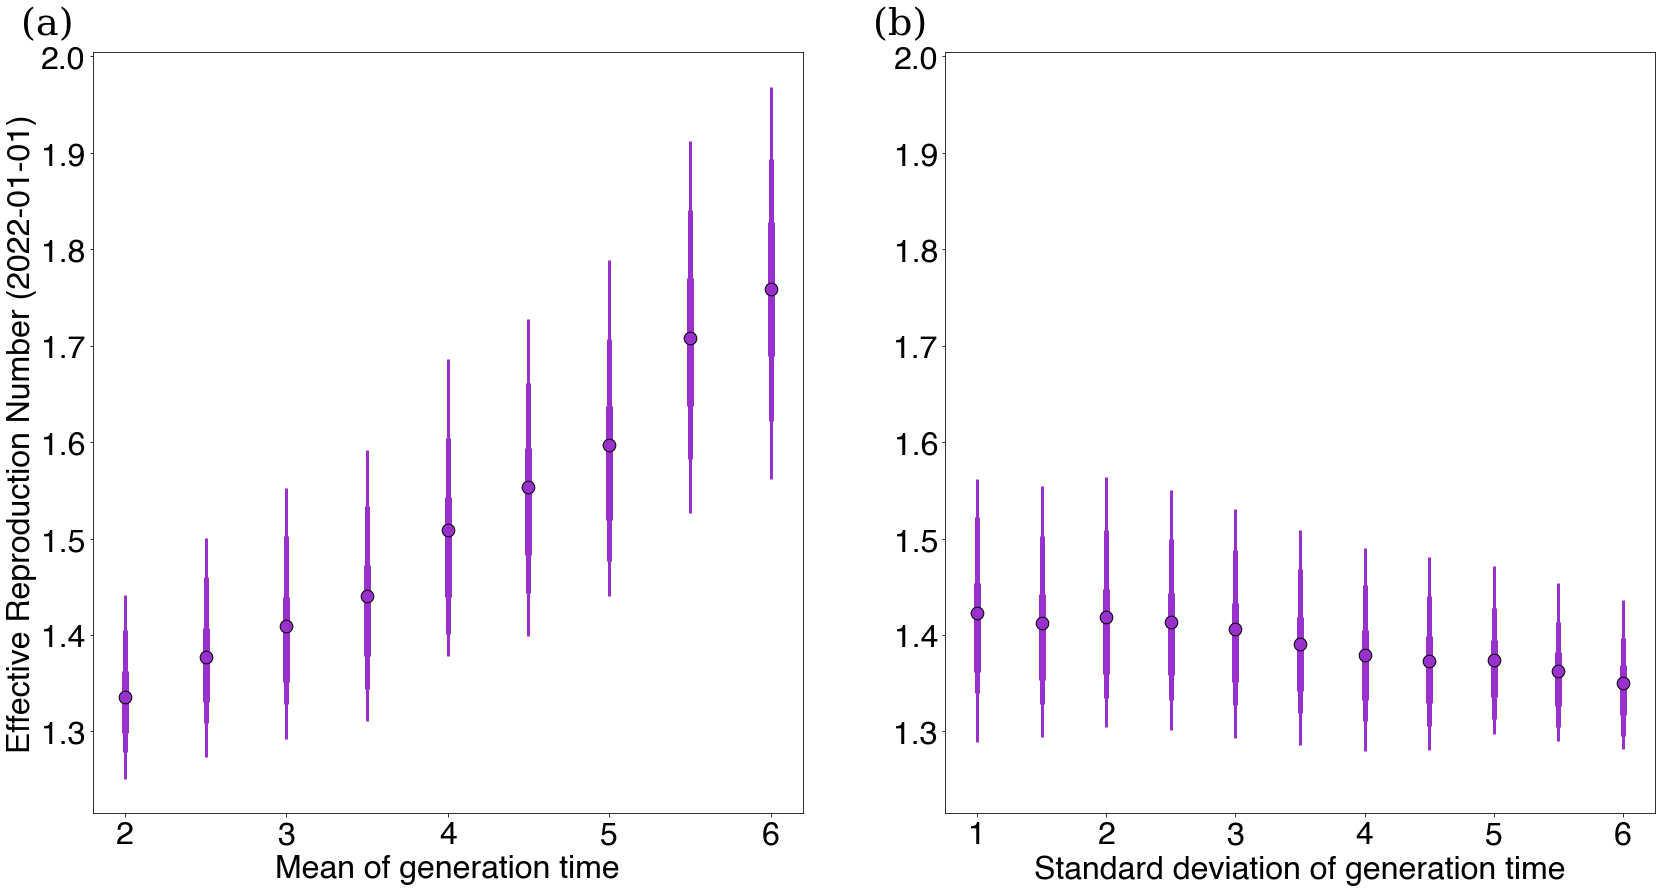
\includegraphics[width=\linewidth]{figs/generation_time_sensitivity.png}
  \caption{\textbf{Sensitivity of effective reproduction number to changes in generation time.}
(a) We vary the mean of Omicron generation time keeping a constant standard deviation 1.2 and plot against effective reproduction number estimates for Omicron in Washington state on February 1st, 2022 using our GARW model.
(b) The same as (a), but we instead vary the standard deviation of Omicron generation time keeping a constant mean 3.1.}%
  \label{fig:generation_time_sensitivity}
\end{figure}

\begin{figure}
  \centering
  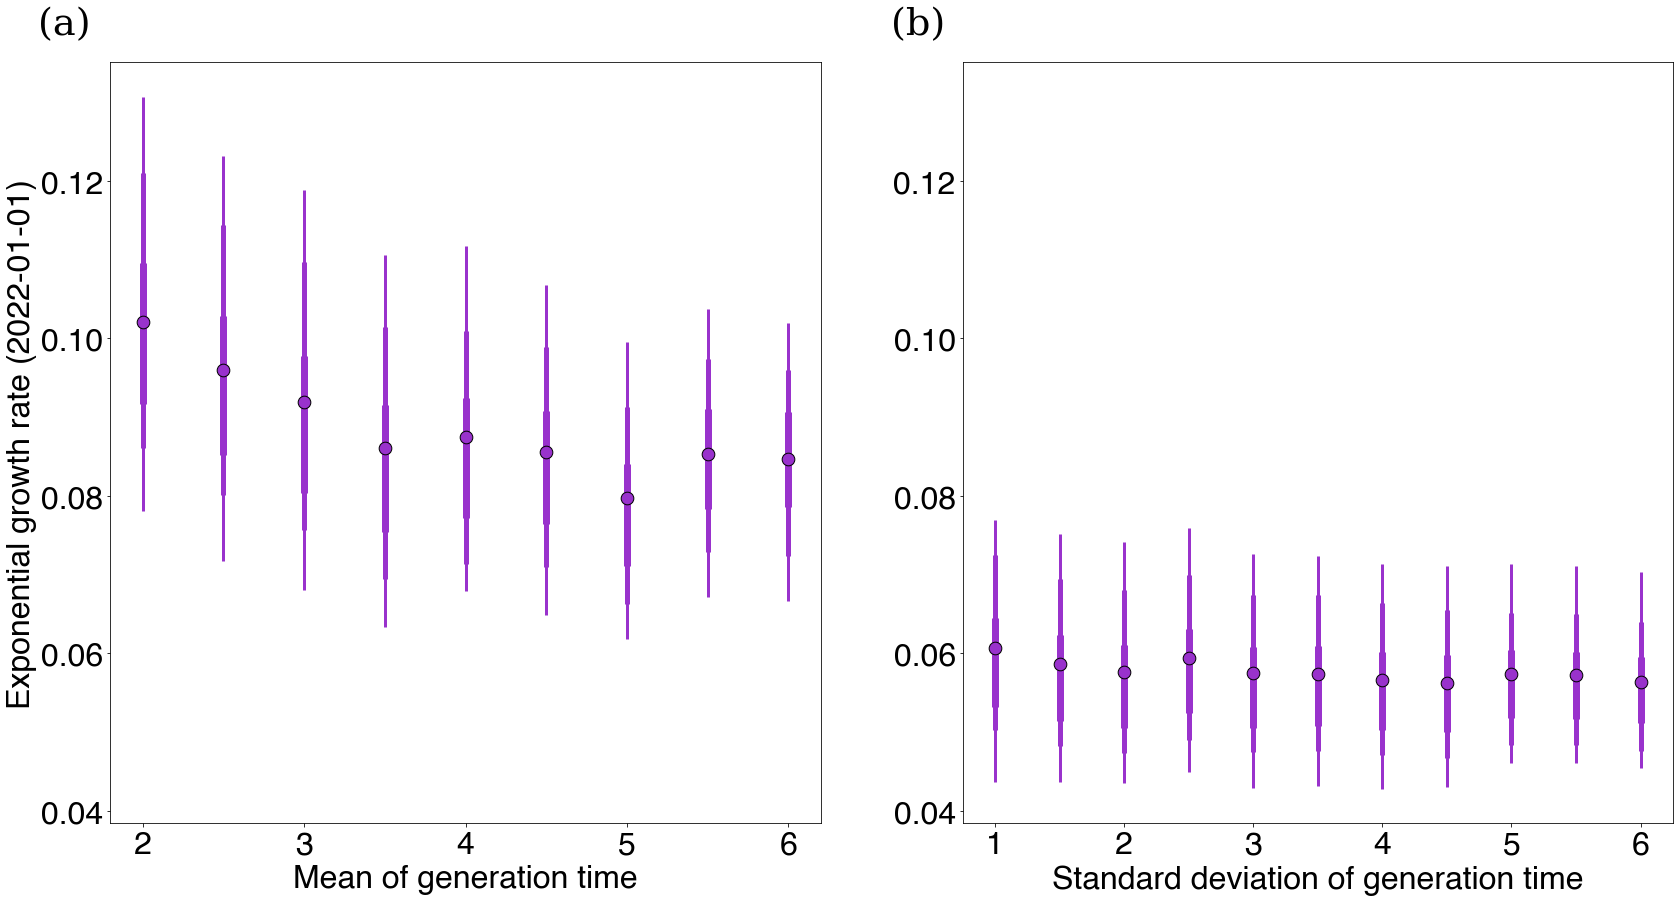
\includegraphics[width=\linewidth]{figs/little_r_sensitivity.png}
  \caption{\textbf{Sensitivity of epidemic growth rates to changes in generation time.}
(a) We vary the mean of Omicron generation time keeping a constant standard deviation 1.2 and plot against exponential growth rates for Omicron in Washington state on February 1st, 2022 using our GARW model and assuming a Gamma-distributed generation time.
(b) The same as (a), but we instead vary the standard deviation of Omicron generation time keeping a constant mean 3.1. }%
  \label{fig:little_r_sensitivity}
\end{figure}

\begin{figure}
  \centering
  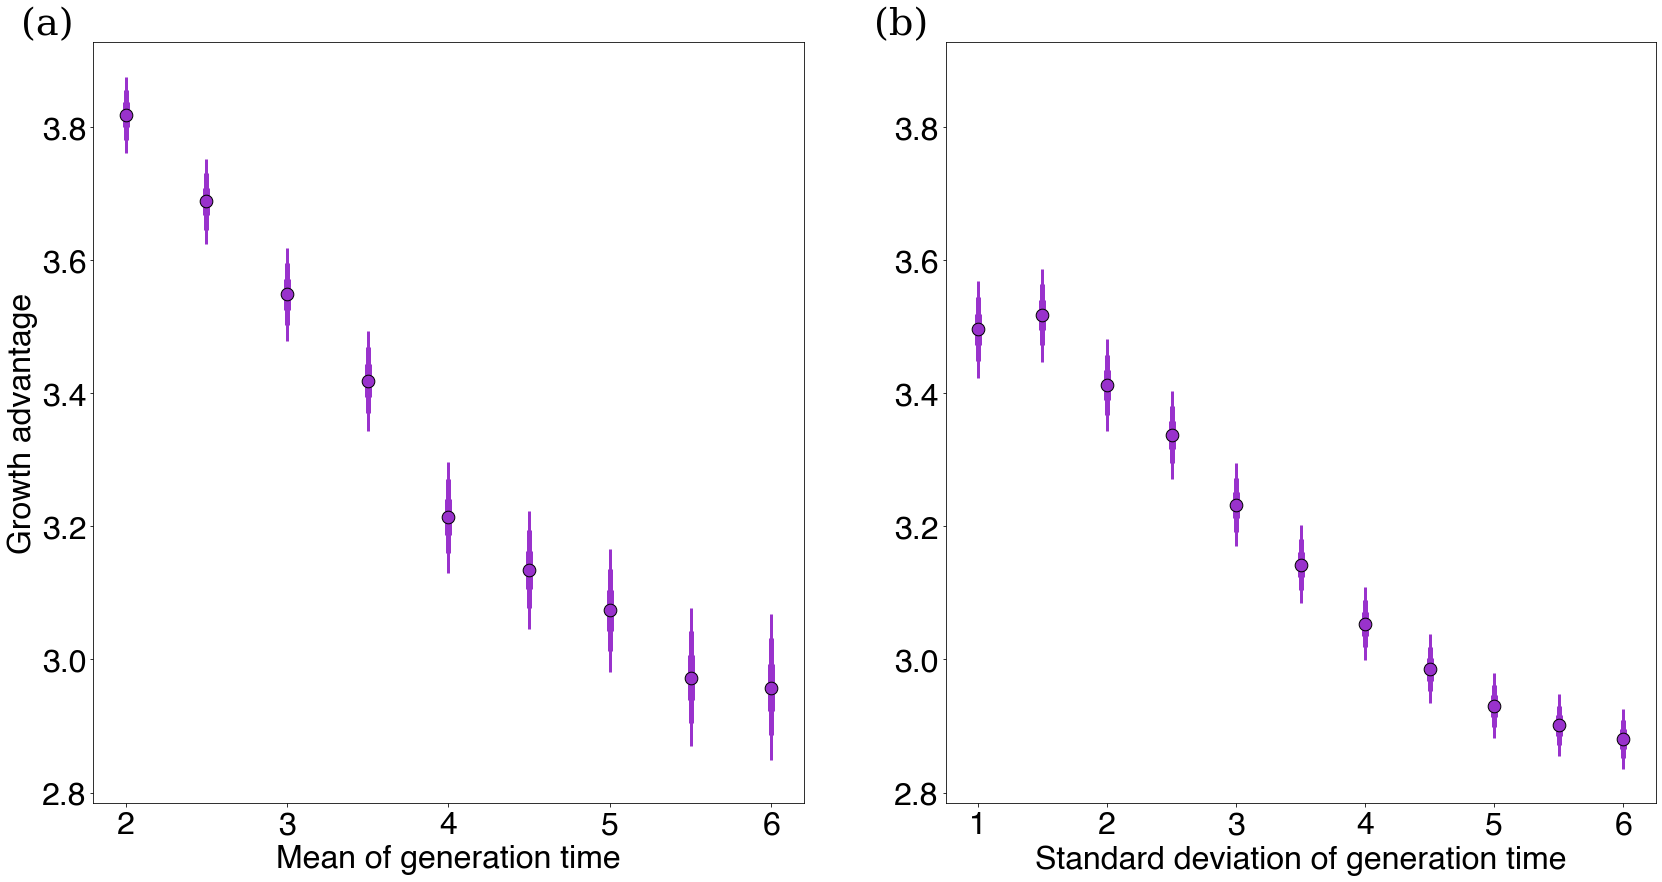
\includegraphics[width=\linewidth]{figs/growth_advantage_sensitivity.png}
  \caption{\textbf{Sensitivity of growth advantages to changes in generation time.}
(a) We vary the mean of Omicron generation time keeping a constant standard deviation 1.2 and plot against exponential growth rates for Delta in Washington state on July 1st, 2021 using our fixed growth model.
(b) The same as (a), but we instead vary the standard deviation of Omicron generation time keeping a constant mean 3.2.}%
  \label{fig:growth_advantage_sensitivity}
\end{figure}

\section{Supplementary Figures}

\begin{figure}
  \centering
  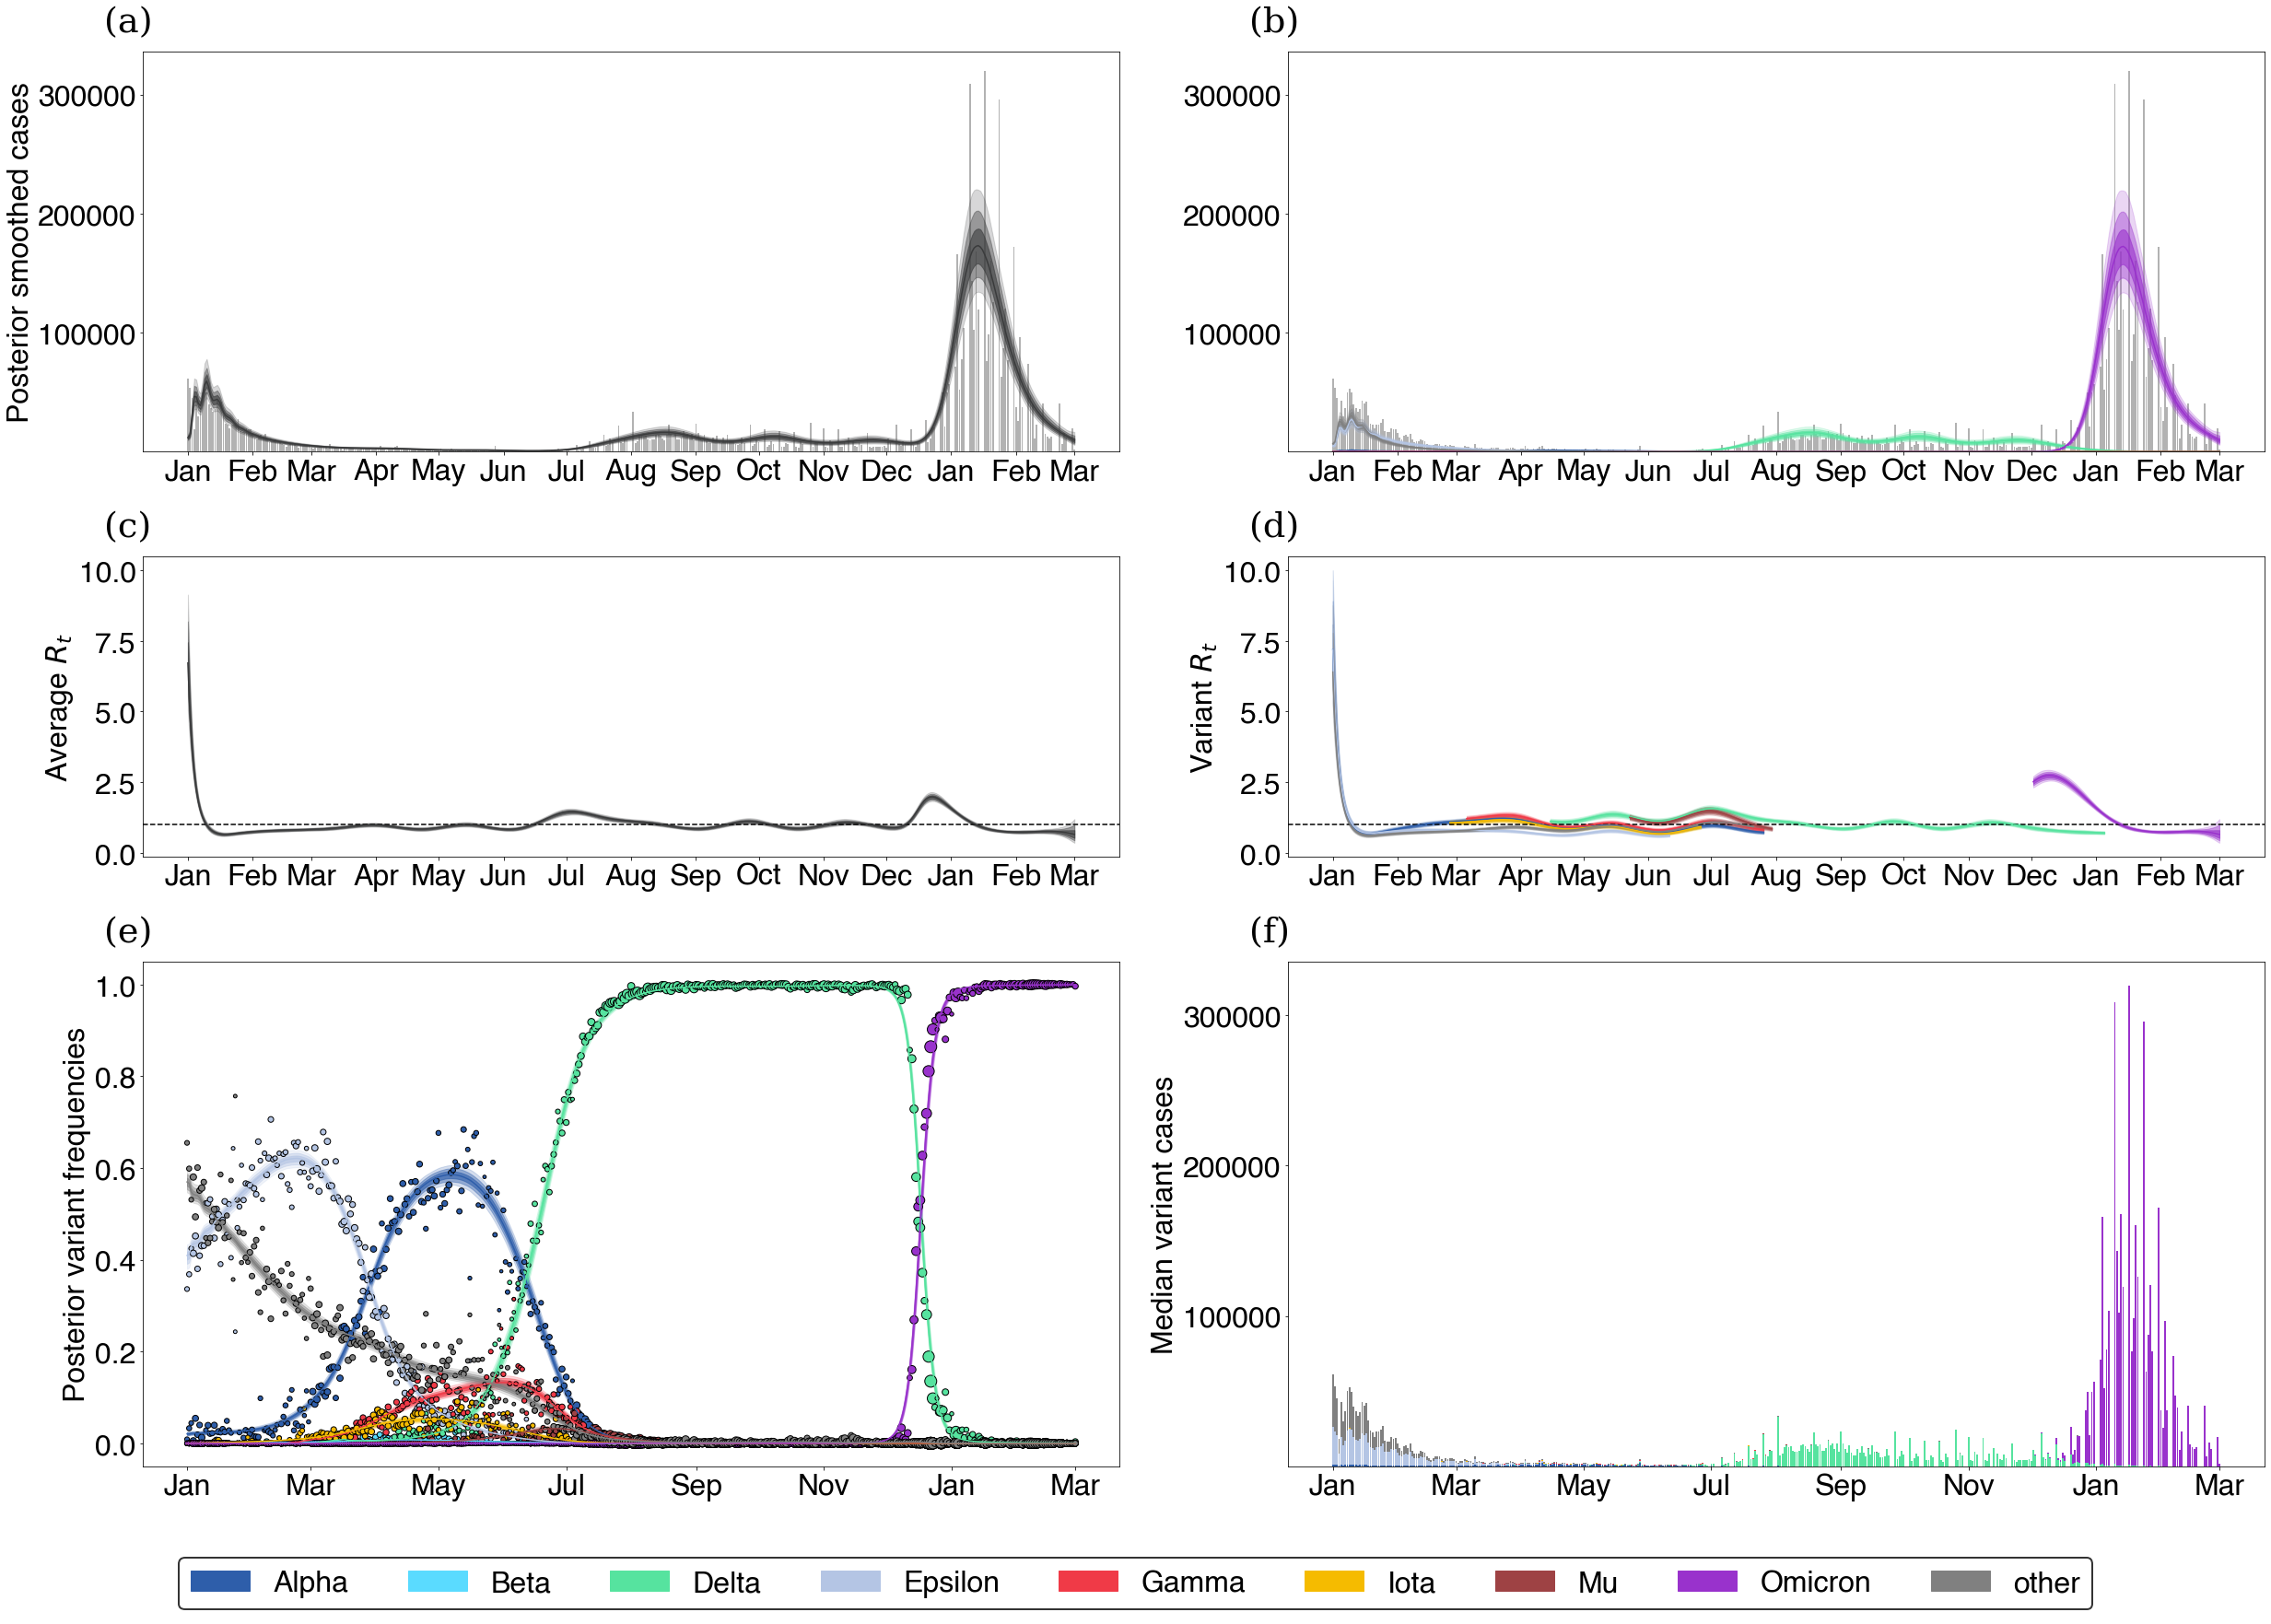
\includegraphics[width=\linewidth]{figs/GARW_rt_California.png}
  \caption{\textbf{Fitting the GARW model to California data.}}%
  \label{fig:GARW_rt_California}
\end{figure}

\begin{figure}
  \centering
  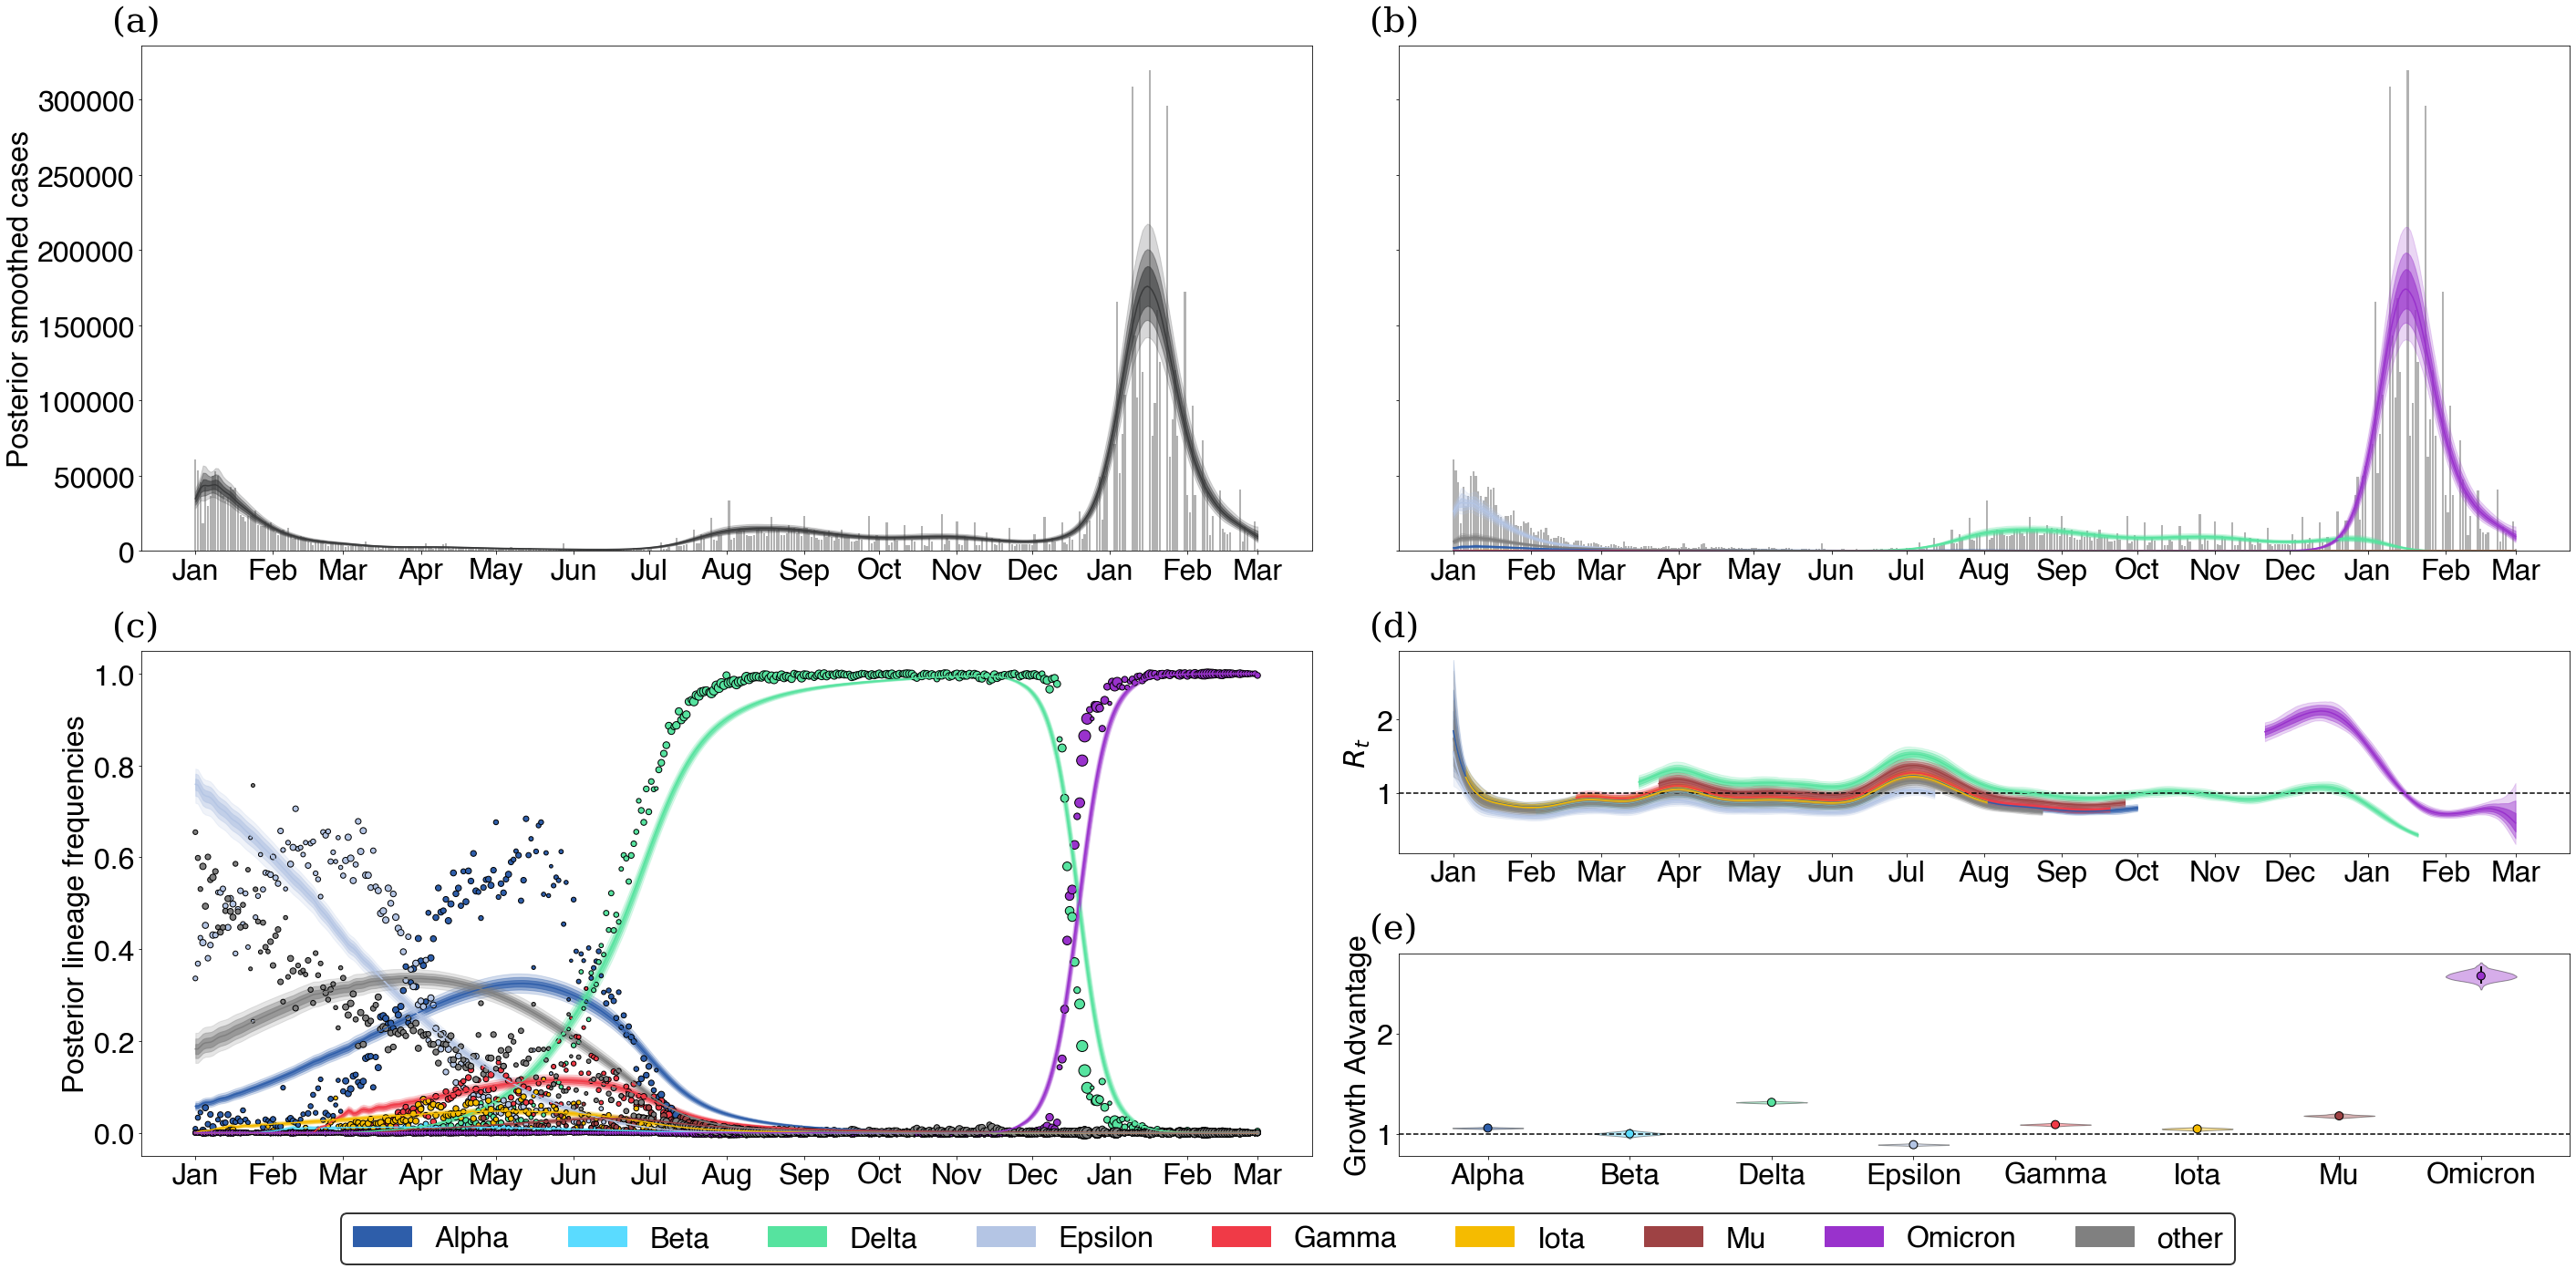
\includegraphics[width=\linewidth]{figs/fixed_growth_California.png}
  \caption{\textbf{Fitting the fixed growth advantage model to California data.}}%
  \label{fig:fixed_growth_California}
\end{figure}

\begin{figure}
  \centering
  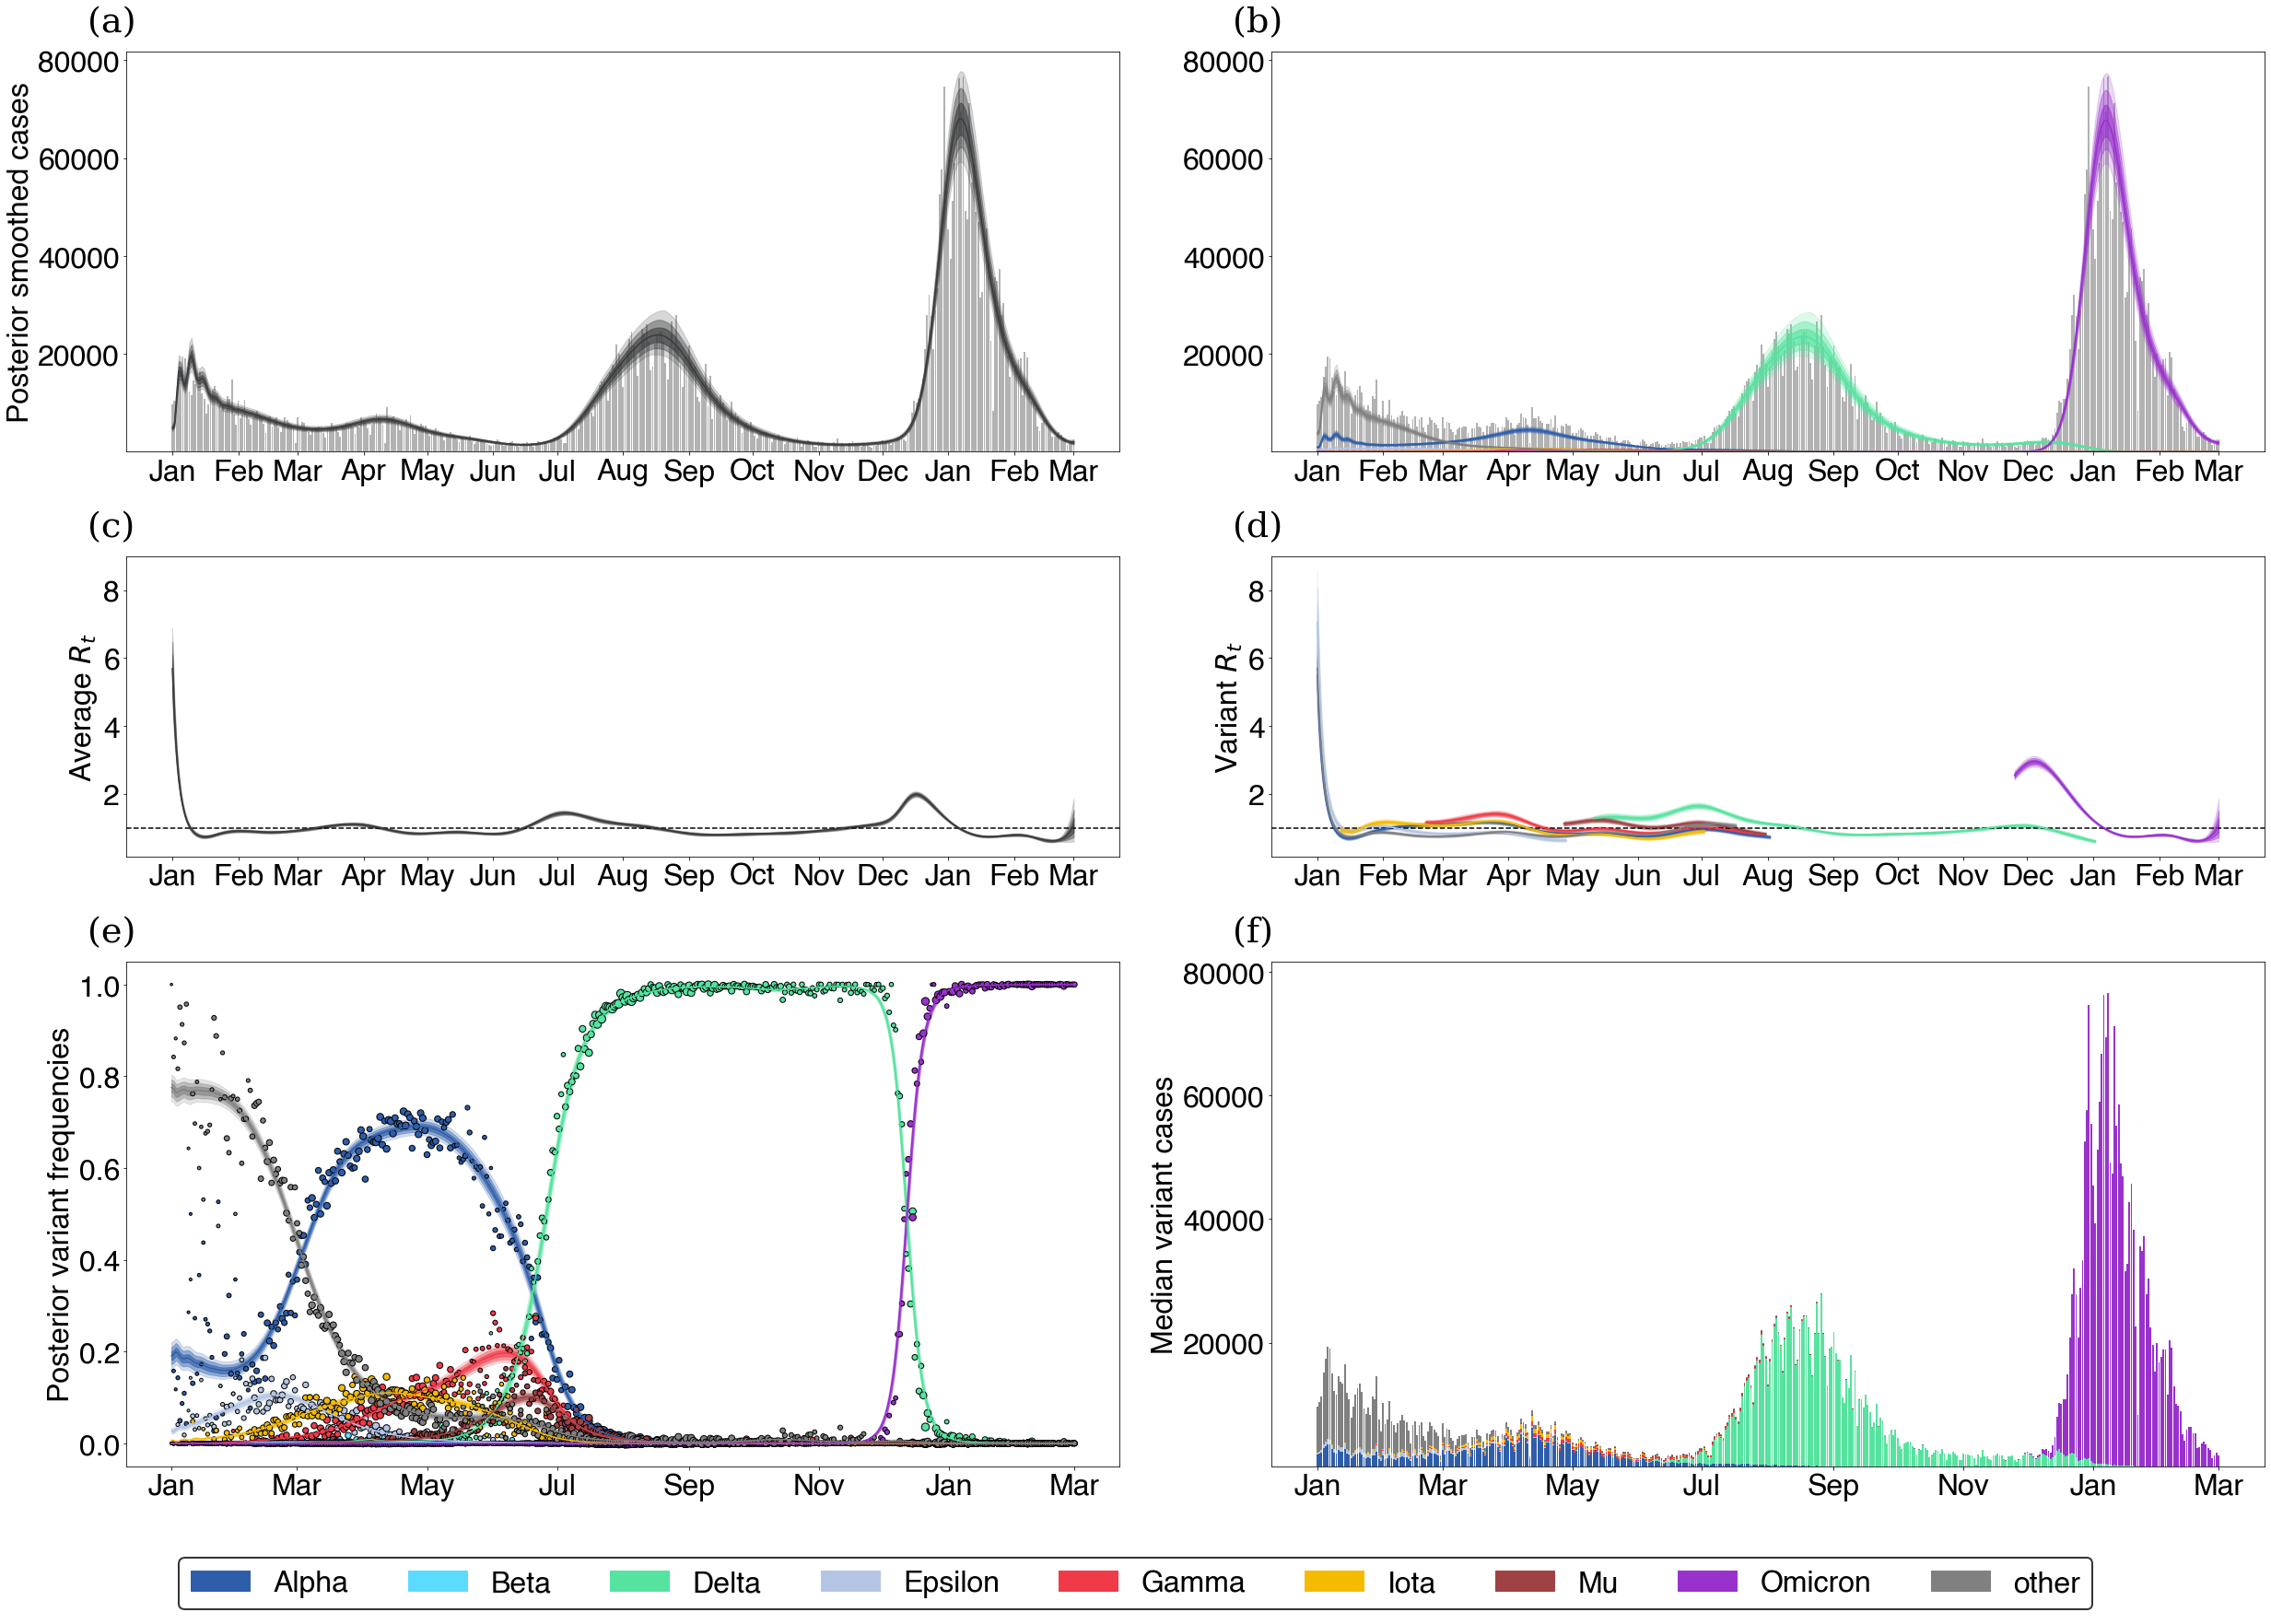
\includegraphics[width=\linewidth]{figs/GARW_rt_Florida.png}
  \caption{\textbf{Fitting the GARW model to Florida data.}}%
  \label{fig:GARW_rt_Florida}
\end{figure}

\begin{figure}
  \centering
  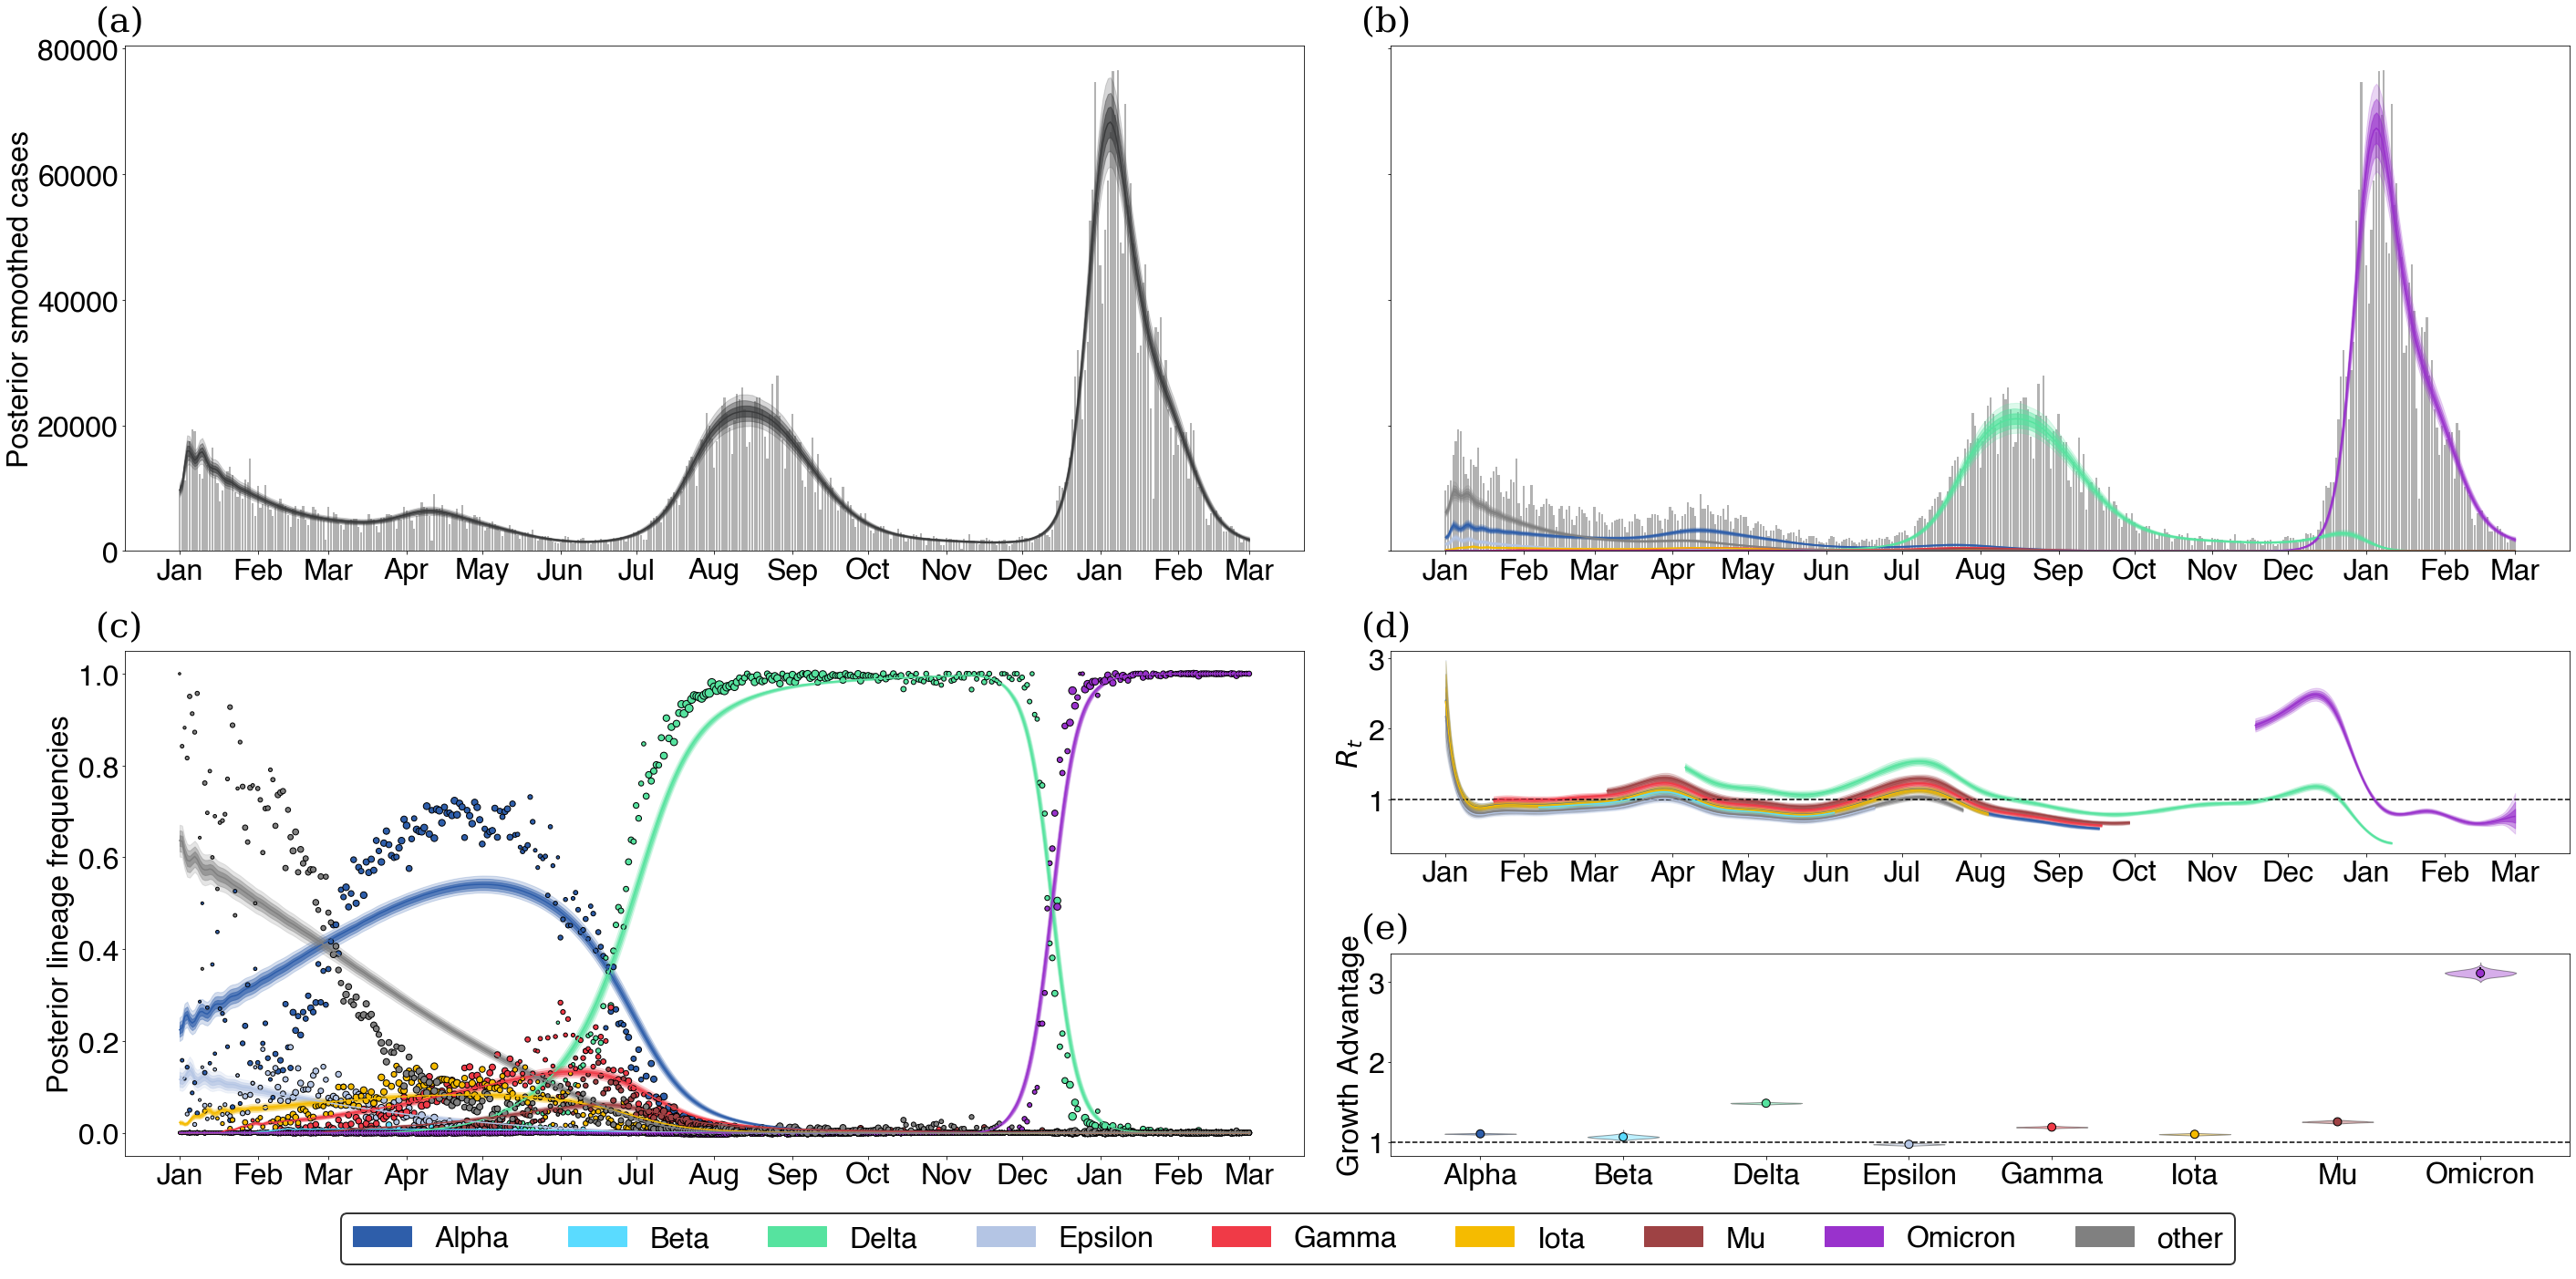
\includegraphics[width=\linewidth]{figs/fixed_growth_Florida.png}
  \caption{\textbf{Fitting the fixed growth advantage model to Florida data.}}%
  \label{fig:fixed_growth_Florida}
\end{figure}

\begin{figure}
  \centering
  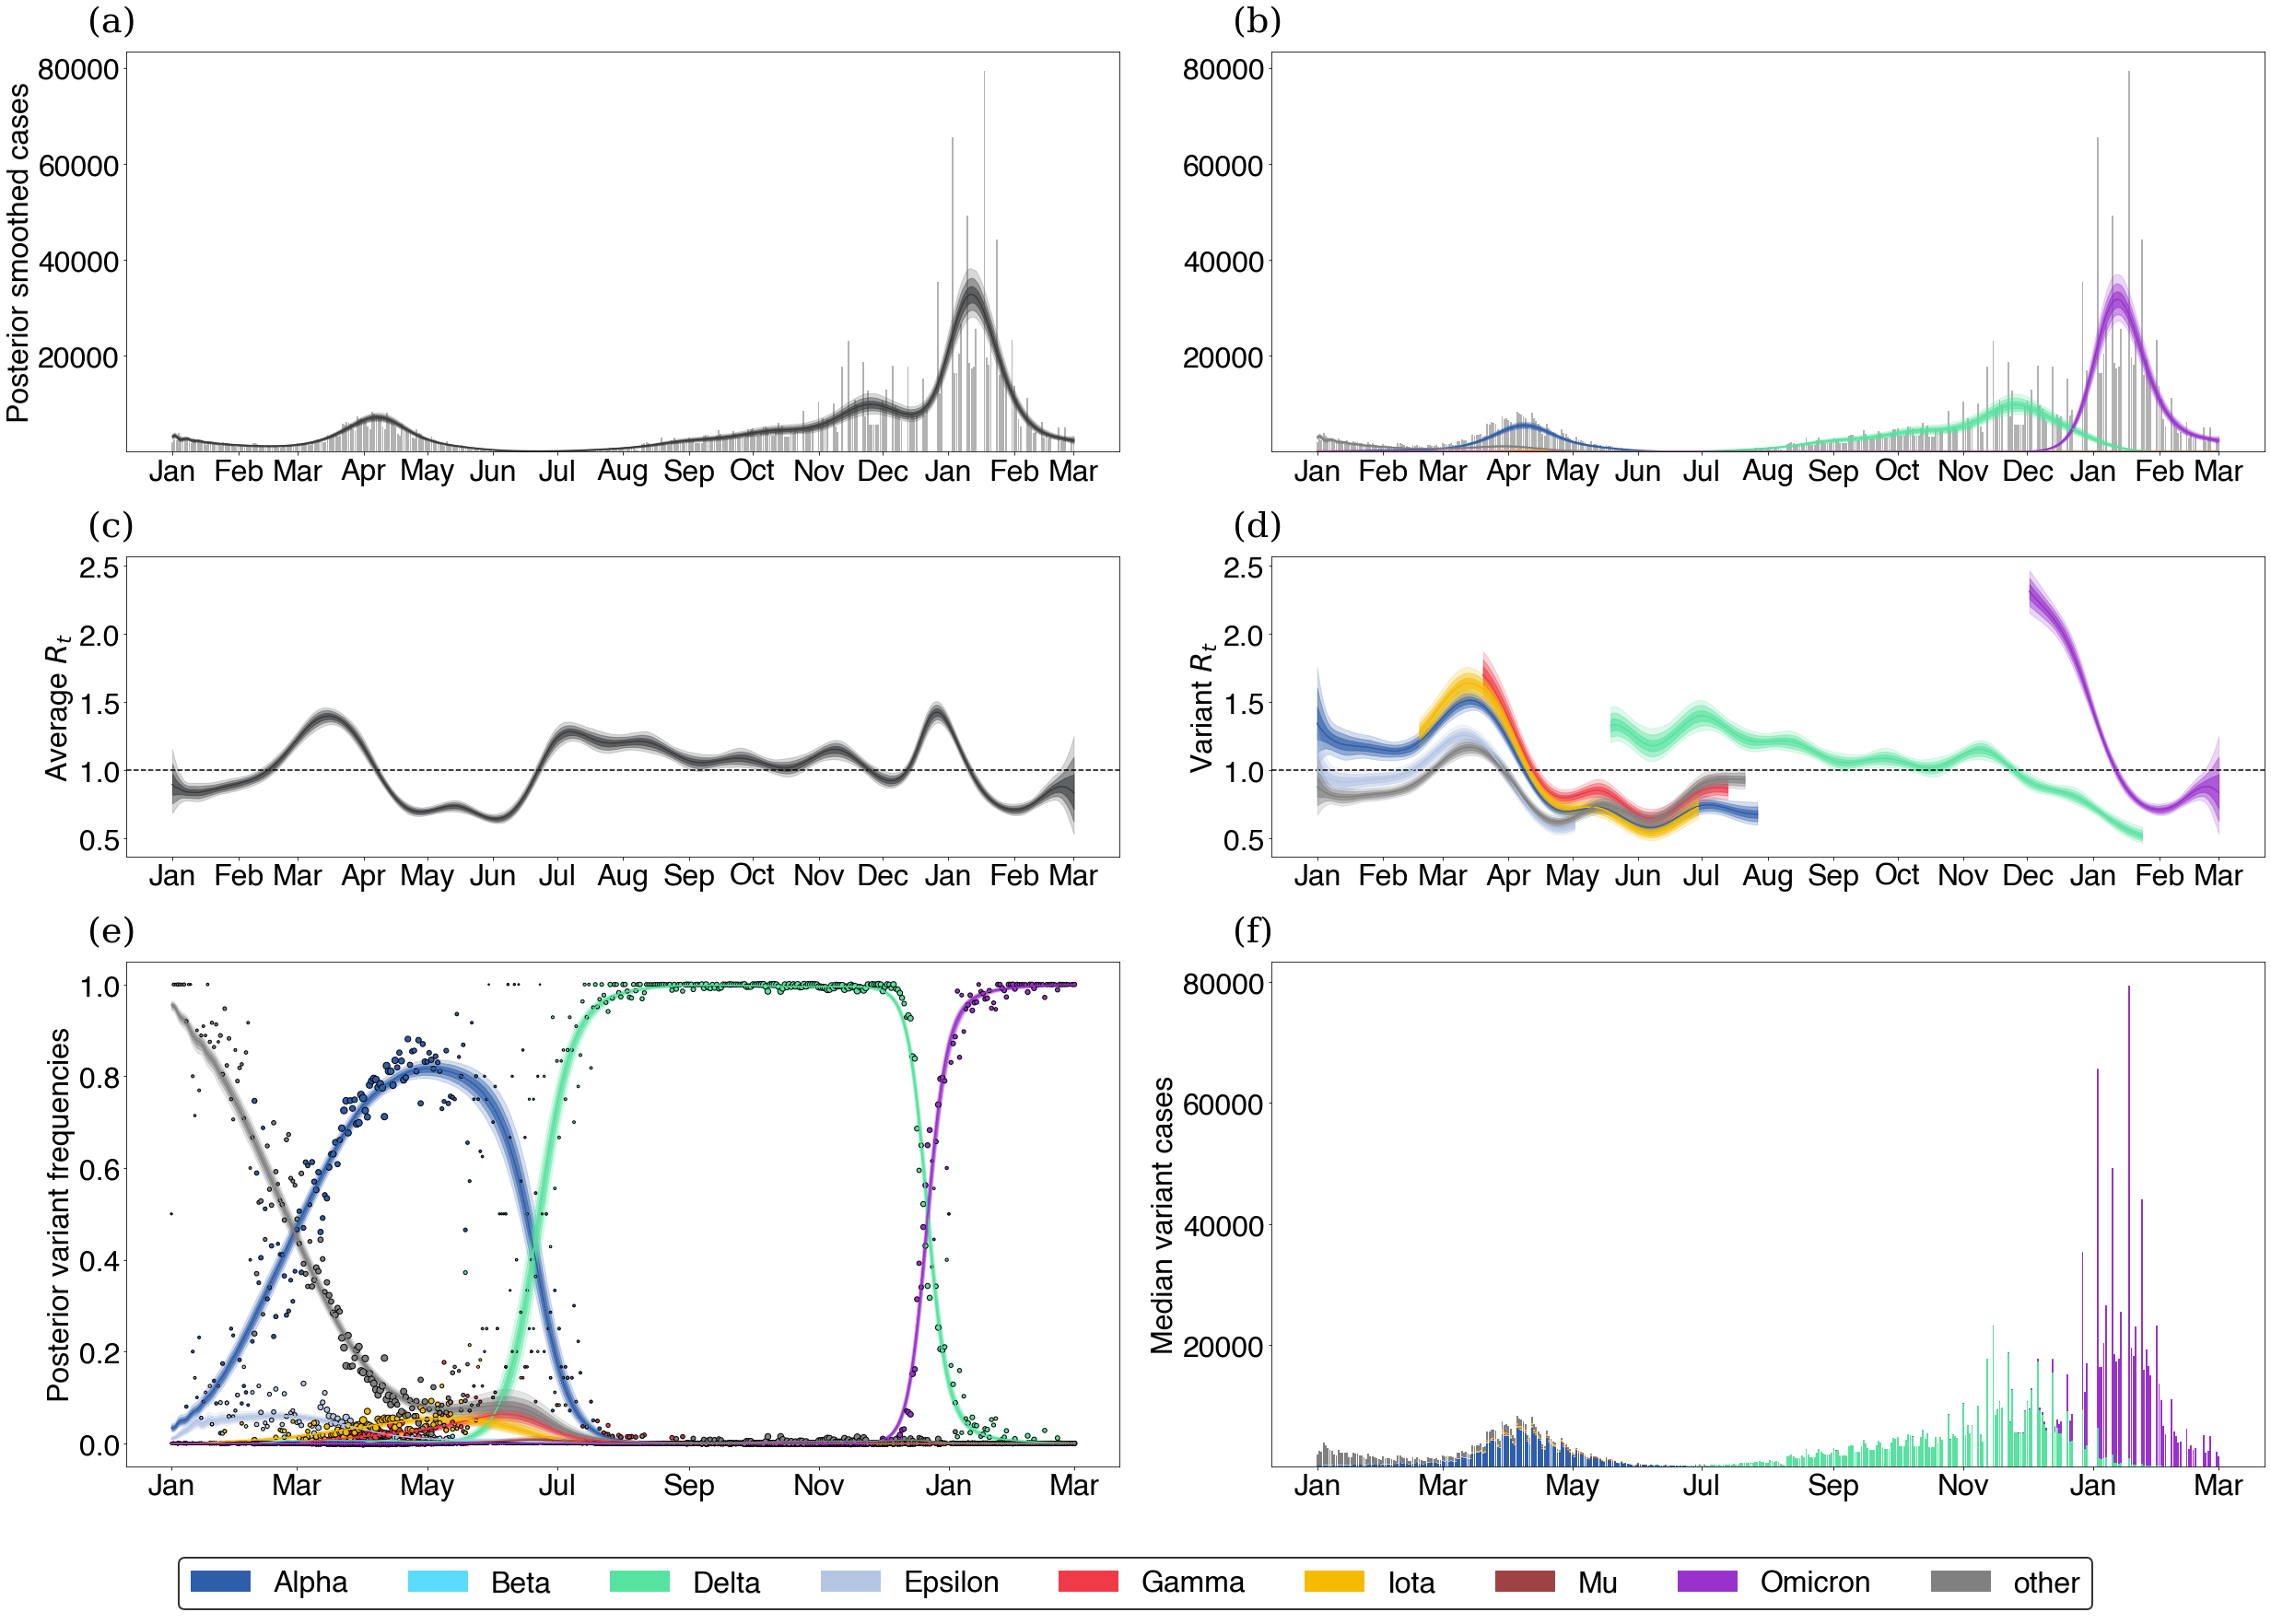
\includegraphics[width=\linewidth]{figs/GARW_rt_Michigan.png}
  \caption{\textbf{Fitting the GARW model to Michigan data.}}%
  \label{fig:GARW_rt_Michigan}
\end{figure}

\begin{figure}
  \centering
  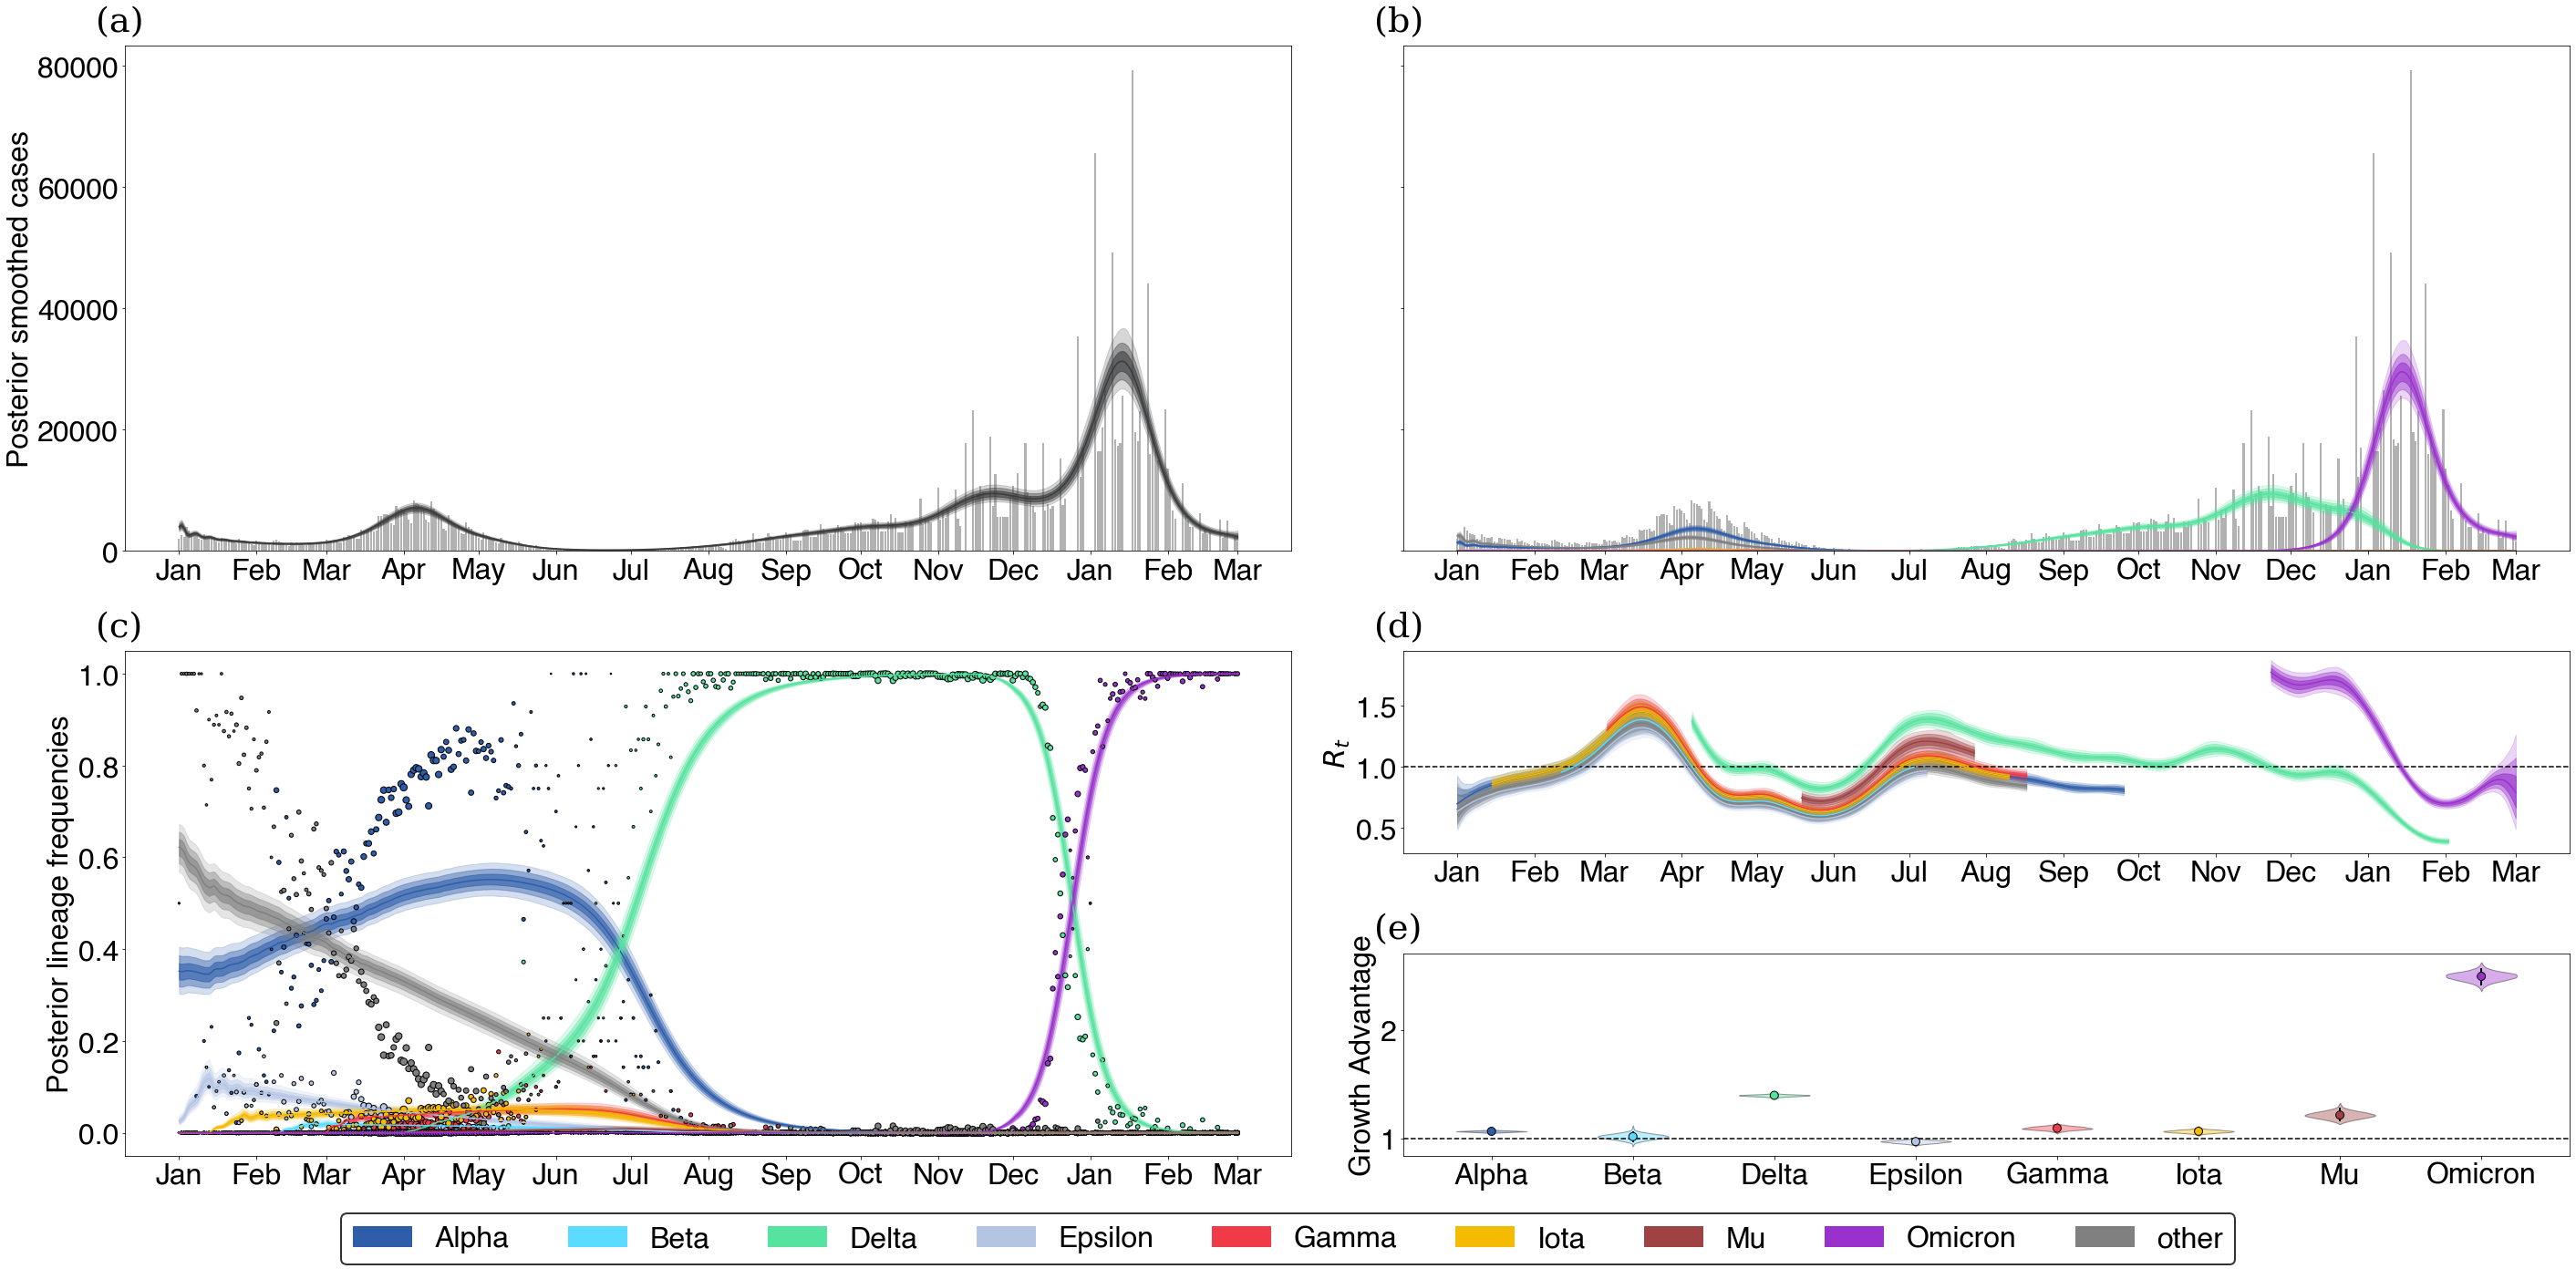
\includegraphics[width=\linewidth]{figs/fixed_growth_Michigan.png}
  \caption{\textbf{Fitting the fixed growth advantage model to Michigan data.}}%
  \label{fig:fixed_growth_Michigan}
\end{figure}

\begin{figure}
  \centering
  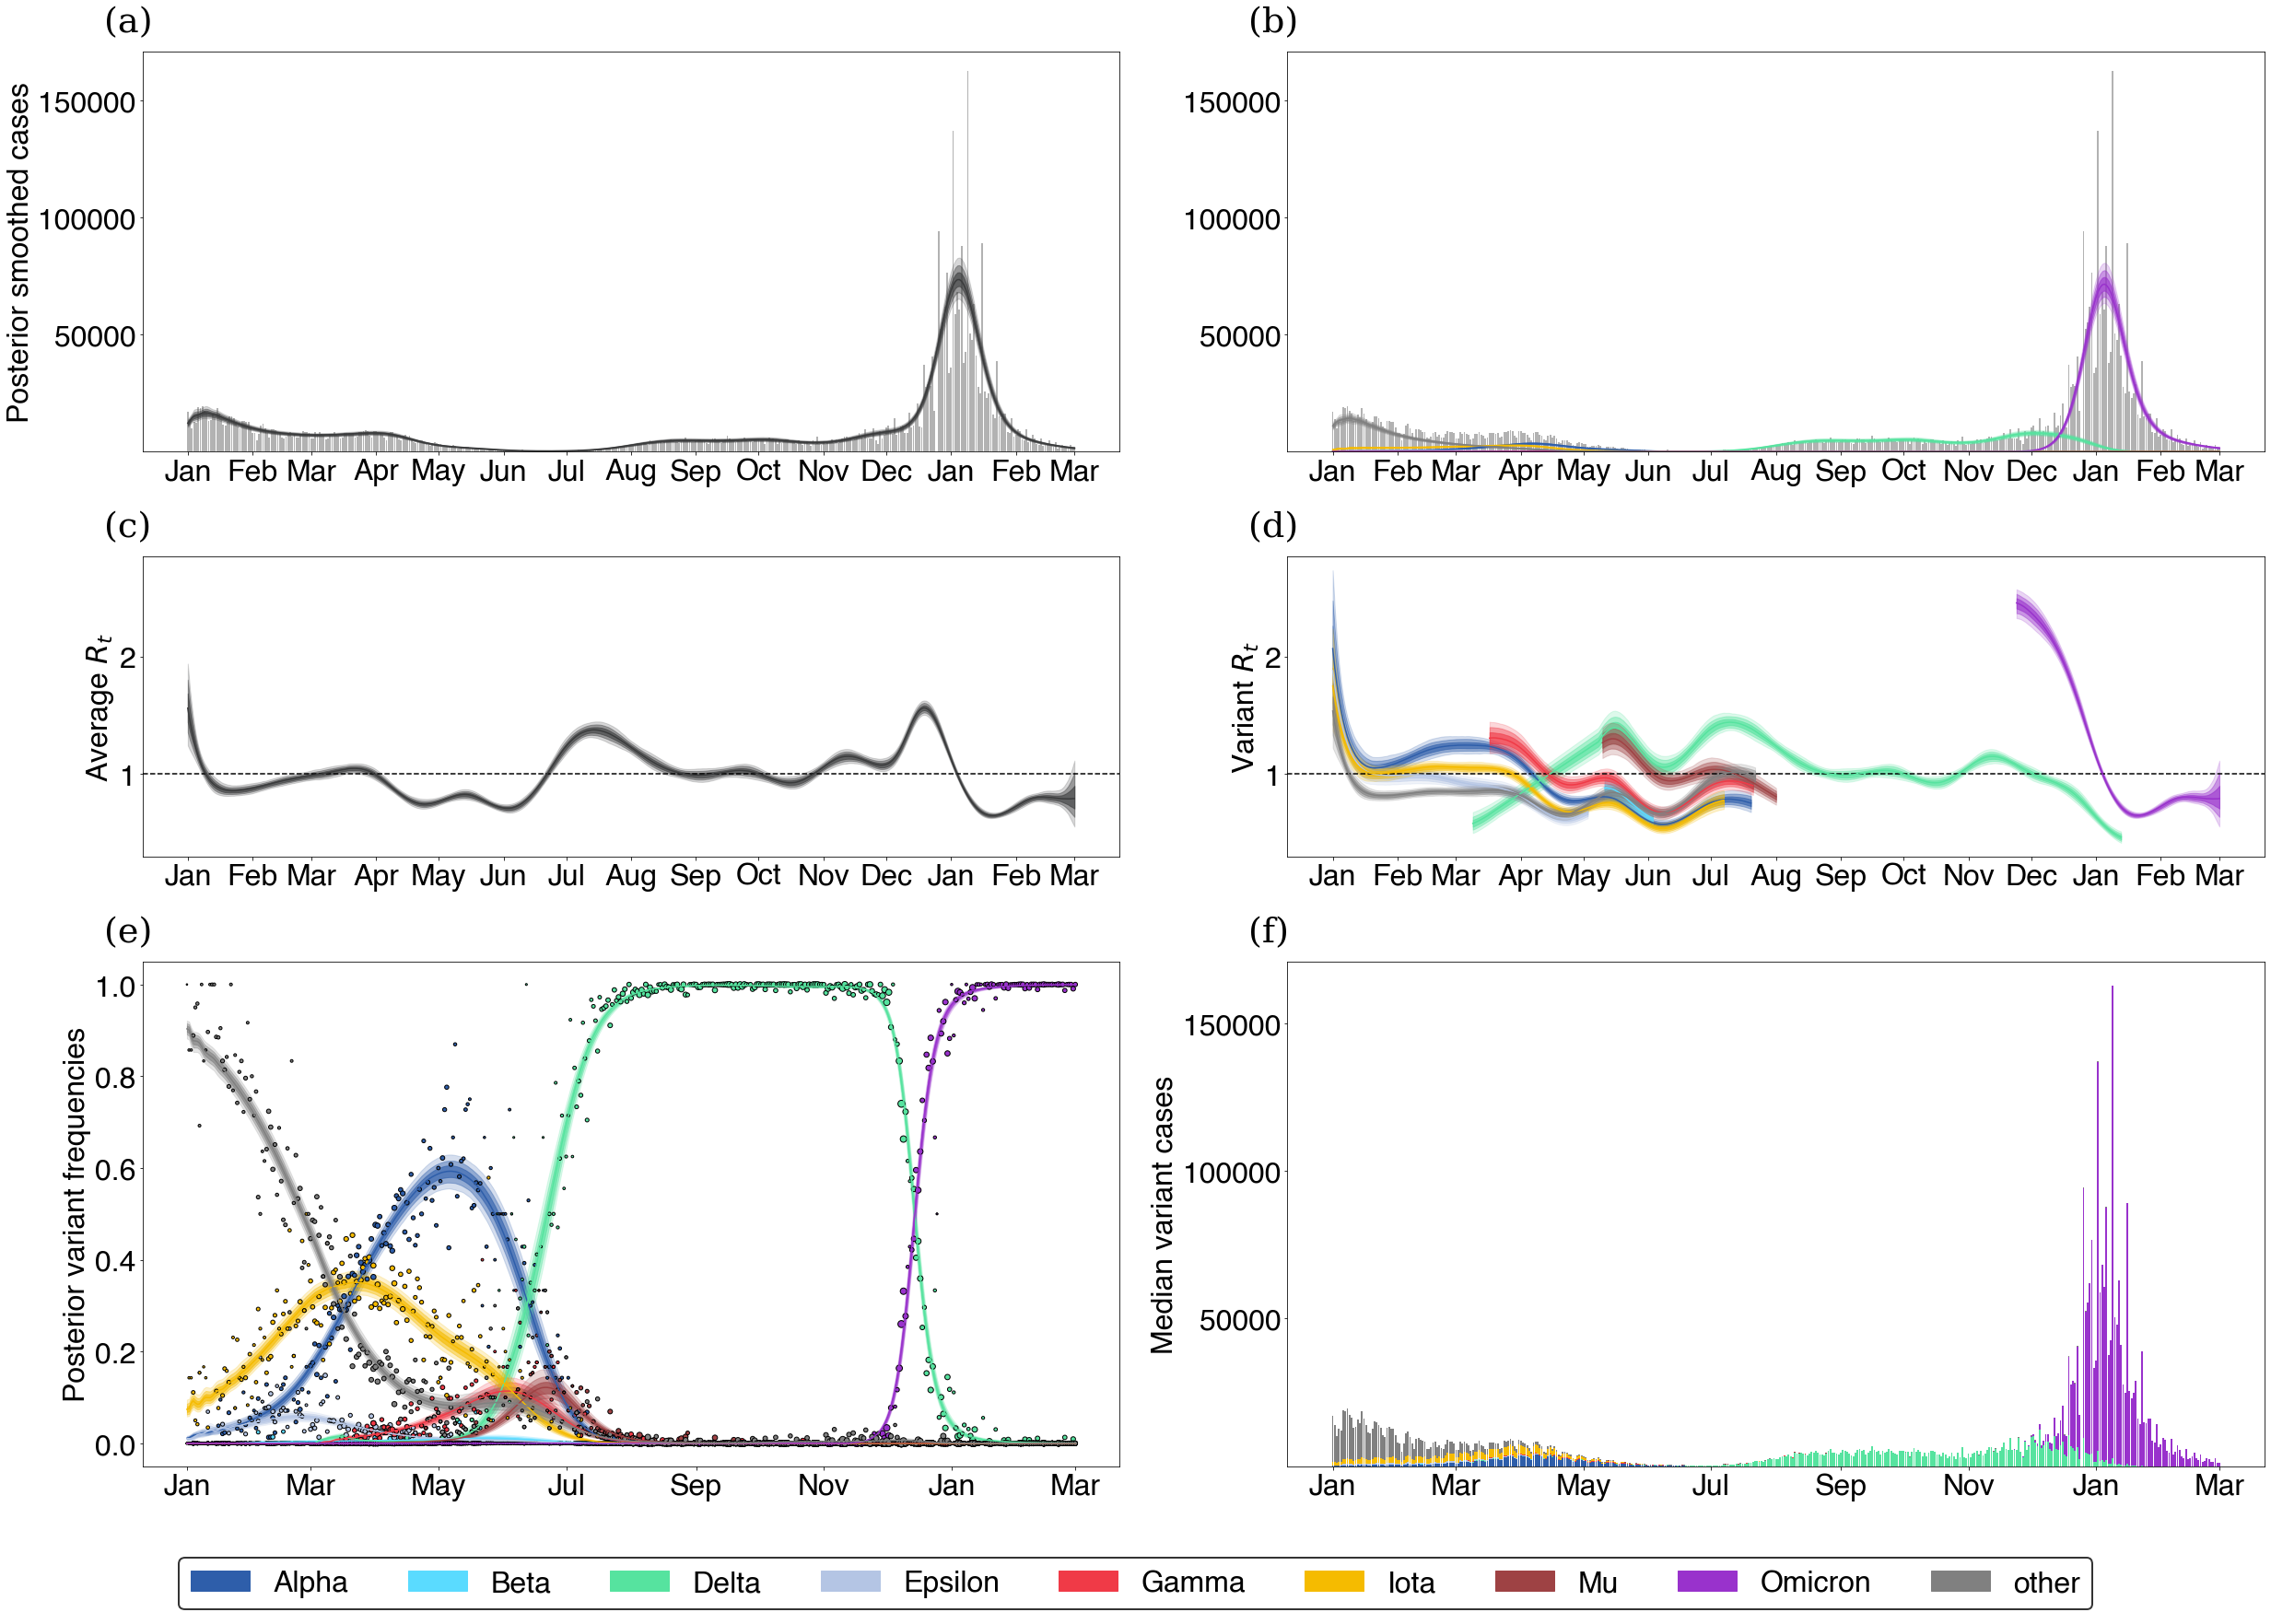
\includegraphics[width=\linewidth]{figs/GARW_rt_New-York.png}
  \caption{\textbf{Fitting the GARW model to New York state data.}}%
  \label{fig:GARW_rt_New-York}
\end{figure}

\begin{figure}
  \centering
  \includegraphics[width=\linewidth]{figs/fixed_growth_New-York.png}
  \caption{\textbf{Fitting the fixed growth advantage model to New York state data.}}%
  \label{fig:fixed_growth_New-York}
\end{figure}

\clearpage


\graphicspath{{./chapters/rt-from-frequency-dynamics/}}
\chapter{Supplementary Materials for Chapter 2} 

%TODO: Make sure we use supplementary results -> supplementary figures

\section{Supplementary Text}

\subsection*{Relationship to multinomial logistic regression}

Other papers have tried to infer growth advantages of variants from sequence data alone, we show that the multinomial logistic regression model typically used in these analysis is roughly equivalent to our fixed growth advantage model, but that inferring relative effective reproduction numbers between variants using multinomial logistic regression requires additional restrictions on the generation time.
Multinomial logistic regression typically models the probability of a given observation belong to class $v$ at time $t$ as
\begin{equation}
  f_{v}(t) = \frac{p_{v}\exp(\beta_{v} t)}{\sum_{1\leq u\leq V} p_{u}\exp(\beta_{u} t)}.
\end{equation}
For our purpose, we can assume this probability is equivalent to the true frequency of variant $v$ in the population and in this case, $p_{v}$ is considered to be related to the prevalence on variant $v$ in the population at $t=0$ and $\beta_{v}$ can be considered to be the growth advantage relative to a pivot class $u_{*}$ which has $\beta_{k_{*}} = 0$.
In order to see the connection between the above model and ours, we return to the original renewal equation of the form
\begin{equation}
  I(t) = R_{t}\int_{0}^{t} I(t-\tau) g(\tau).
\end{equation}
Assuming that $g$  is a point mass at a mean generation time $T_{g}$, we have that
\begin{equation}
  I(nT_{g}) = \left(\prod_{i=1}^{n} R_{iT_{g}}\right) I(0).
\end{equation}
Assuming that there are several variants following these same dynamics, we have that the frequency of a given variant $v$ can be written as
\begin{equation}
  f_{v}(nT_{g}) = \frac{I_{v}(nT_{g})}{\sum_{1\leq u \leq V} I_{u}(nT_{g})}.
\end{equation}
If we assume a constant growth advantage as in our model, we then have that $R_{t,v} = \Delta_{v} R_{t}$, so that
\begin{equation}
  f_{v}(nT_{g}) =  \frac{\Delta_{v}^{n} I_{v}(0)}{\sum_{1\leq u \leq V} \Delta_{u}^{n} I_{u}(0)}.
\end{equation}
Writing $\Delta_{v} = \exp(\delta_{v})$ and $t = n T_{g}$, allows us to see that
\begin{equation}
  f_{v}(t) = \frac{I_{v}(0) \exp(\frac{\delta_{v}}{T_{g}} t)}{\sum_{1\leq u \leq V}I_{u}(0) \exp(\frac{\delta_{u}}{T_{g}} t)}.
\end{equation}
By fixing one pivot class so that $I_{u_{*}} = 1$ and $\delta_{u_{*}} / T_{g} = 0$, we can identify our model with the multinomial logistic regression by relating the parameters as

\begin{align}
  \delta_{v} &= \beta_{v}T_{g}\\
  I_{v}(0) &= p_{v}.
\end{align}

This shows that the multinomial logistic regression functions similarly to our fixed growth advantage model except with the additional assumption that the generation time is a point mass at $T_{g}$.
This assumption additionally allows us to relate the epidemic growth rate $r$ and the effective reproduction number as $R = \exp(r T_{g})$ \cite{Wallinga2006}.
Therefore, by further assuming that the variant infections are exponentially growing with rates $r_{v}$, we can then identify $\beta_{v} = r_{v} - r_{u_{*}}$.
This means that the relative effective reproduction number for any two variants can be written as
\begin{align*}
\ln \left( \frac{R_{t,v}}{R_{t,u}} \right) = (\beta_{v} - \beta_{u}) T_{g}.
\end{align*}

\begin{figure}
  \centering
  \includegraphics[width=\linewidth]{figs/fig_MLR_growth_advantages_supp.png}
  \caption{Estimating variant growth advantages in various states using Multinomial Logistic Regression model assuming generation time $T_{g} = 5.2$.
  (a) Growth advantages visualized by state.
  (b) Same as (a) but grouped by variant.}%
  \label{fig:MLR_growth_advantages}
\end{figure}

\newpage

\subsection*{Relating epidemic growth rates to relative effective reproduction numbers}

An important relationship of interest is between the epidemic growth rate of an epidemic and its effective reproduction number.
In the case of our analysis, we are particularly interested in the effect of generation time assumptions on estimated variant-specific effective reproduction numbers.
First, notice that the effective reproduction number and the epidemic growth rate of an epidemic are related by
\begin{align*}
R_{t} = \frac{1}{\int_{0}^{\infty} \exp(-r\tau)g(\tau)d\tau} = \frac{1}{M_{g}(-r)}
\end{align*}
according to the Lotka-Euler equation \cite{Wallinga2006} where $r$ is the epidemic growth rate and $M_{g}$ is the moment-generating function of the generation time $g$.

This allows us to write the relative reproduction number of two variants $v$ and $u$ as a function of their epidemic growth rates, so that
\begin{align*}
\frac{R_{t,v}}{R_{t,u}} = \frac{M_{g}(-r_{u})}{M_{g}(-r_{v})}.
\end{align*}

We'll consider three common generation time assumptions. First, we consider the case where the generation time is a point mass at $T_{g}$. In which case, $M_{g}(-r) = \exp(-r T_{g})$ and we recover the relationship
\begin{align*}
R_{t,v} = \exp(r_{v}T_{g}).
\end{align*}

In this case, the relative effective reproduction number will depend on only the difference between the epidemic growth rates and therefore, is commonly used when converting estimated growth advantages to relative reproduction numbers in the case of logistic growth models.

Second, we consider the case where the generation time is an exponential distribution with mean $T_{g}$. This assumption is often implicit and common in models of infectious diseases such as ODEs and their stochastic variants. Using the corresponding moment-generating function, we see that
\begin{align*}
R_{t,v} = 1 + r_{v} T_{g}
\end{align*}

Next, we consider the Gamma distributed generation times with mean $T_{g}$ and standard deviation $s$.
This is often used in models of infectious diseases via the chain trick in which multiple compartments are chained together to obtain non-exponential generation times or infectious periods.
Re-parameterizing the Gamma distribution in terms of its mean and standard deviation and using its moment generating function, we have that
\begin{align*}
R_{t,v} = \left(1 + r_{v}  \left(\frac{s^{2}}{T_{g}}\right) \right)^{T_{g}^{2} / s^{2}}.
\end{align*}

From this equation, we can see that increases in the mean of the generation time of $v$ leads to decreasing estimates of $R_{t,v}$ during epidemic decline ($r_{v} < 0$) and increased estimates during epidemic growth ($r_{v} > 0$) assuming $r_{v}$ and $s$ are fixed.
Additionally, increases in the standard deviation will generally lead to lower inferred variant advantages.
This effect is also visualized in Figure \ref{fig:generation_time_sensitivity}.

\paragraph{Variant growth-advantages are sensitive to generation time}%

In the case where we have two variants $u, v$ with Gamma-distributed generation times with means $T_{u}, T_{v}$ and standard deviations $s_{u}, s_{v}$ respectively, we can then write the relative effective reproduction number of $v$ over $u$ as
\begin{align*}
\frac{R_{t,v}}{R_{t,u}} = \frac{\left[1 + r_{v}  \left(\frac{s_{v}^{2}}{T_{v}}\right)\right]^{T_{v}^{2} / s_{v}^{2}}}{\left[1 + r_{u} \left(\frac{s_{u}^{2}}{T_{u}}\right)\right]^{T_{u}^{2} / s_{u}^{2}}}.
\end{align*}
It follows that increases in the mean of the generation time of $v$ leads to decreasing inferred variant advantages during epidemic decline and increased advantages during epidemic growth when all quantities are fixed.
On the other hand, increases in the standard deviation will generally lead to lower inferred variant advantages.

Taking a logarithm, we can also evaluate the sensitivity of our inferred growth advantages from our fixed growth advantage model with respect to the generation time assuming it is Gamma distributed as
\begin{align*}
 \delta_{v}  = \ln \left( \frac{R_{t,v}}{R_{t,0}} \right) = \left( \frac{T_{g}^{2}}{s^{2}} \right)  \ln \left( \frac{1 + r_{v}  \left(\frac{s^{2}}{T_{g}}\right)}{1 + r_{0} \left(\frac{s^{2}}{T_{g}}\right) } \right).
\end{align*}
As the log of the relative effective reproduction number, the behavior here is analogous to that discussed above when the mean $T_{g}$ and standard deviation $s$ are changed.
This effects of varying mean and standard deviation are illustrated in Figure \ref{fig:growth_advantage_sensitivity}.
Although the effective reproduction number and the growth advantage appear to have strong dependence on generation time parameters, we find that the epidemic growth rate $r$ is more robust to changes in generation time (see Figure \ref{fig:little_r_sensitivity}).

The cases of exponential and Gamma-distributed generation times highlight that for non-deterministic generation times there is no guarantee that the relative effective reproduction number depends on only the difference in epidemic growth rates.
In fact, these estimates based on the deterministic generation times correspond to the case in which the standard deviation shrinks zero, they are likely overestimates of variant advantages given the observed variation in the serial interval of SARS-CoV-2 infections.

\paragraph{Fixed growth advantages become time-varying under generation time misspecification}

We'll now consider the case where there is a true fixed-variant growth advantage. Suppose for a two-variant system that $\delta$ is the constant (log) growth advantage of the variant virus over the wildtype under the variant generation time $g_{T}$, so that $\delta = \ln \left( R_{t,v}^{g_{T}} / R_{t, wt}^{g_{T}} \right)$.
Here subscripts denote the generation time used when computing $R_{t}$.

Under the misspecified variant generation time $g_{M}$, we can then write the inferred growth advantage as
\begin{align*}
  \delta_{M} &= \ln \left( \frac{R_{t,v}^{g_{M}}}{R_{t, wt}^{g_{T}}} \right) = \ln \left(\frac{R_{t,v}^{g_{M}}}{R_{t,v}^{g_{T}}}\right) + \delta.
\end{align*}

In general, the term inside the log is non-constant meaning that fixed variant growth advantages under one generation time become non-constant under generation time specification.

\begin{figure}
  \centering
  \includegraphics[width=\linewidth]{figs/generation_time_sensitivity.png}
  \caption{\textbf{Sensitivity of effective reproduction number to changes in generation time.}
(a) We vary the mean of Omicron generation time keeping a constant standard deviation 1.2 and plot against effective reproduction number estimates for Omicron in Washington state on February 1st, 2022 using our GARW model.
(b) The same as (a), but we instead vary the standard deviation of Omicron generation time keeping a constant mean 3.1.}%
  \label{fig:generation_time_sensitivity}
\end{figure}

\begin{figure}
  \centering
  \includegraphics[width=\linewidth]{figs/little_r_sensitivity.png}
  \caption{\textbf{Sensitivity of epidemic growth rates to changes in generation time.}
(a) We vary the mean of Omicron generation time keeping a constant standard deviation 1.2 and plot against exponential growth rates for Omicron in Washington state on February 1st, 2022 using our GARW model and assuming a Gamma-distributed generation time.
(b) The same as (a), but we instead vary the standard deviation of Omicron generation time keeping a constant mean 3.1. }%
  \label{fig:little_r_sensitivity}
\end{figure}

\begin{figure}
  \centering
  \includegraphics[width=\linewidth]{figs/growth_advantage_sensitivity.png}
  \caption{\textbf{Sensitivity of growth advantages to changes in generation time.}
(a) We vary the mean of Omicron generation time keeping a constant standard deviation 1.2 and plot against exponential growth rates for Delta in Washington state on July 1st, 2021 using our fixed growth model.
(b) The same as (a), but we instead vary the standard deviation of Omicron generation time keeping a constant mean 3.2.}%
  \label{fig:growth_advantage_sensitivity}
\end{figure}

\section{Supplementary Figures}

\begin{figure}
  \centering
  \includegraphics[width=\linewidth]{figs/GARW_rt_California.png}
  \caption{\textbf{Fitting the GARW model to California data.}}%
  \label{fig:GARW_rt_California}
\end{figure}

\begin{figure}
  \centering
  \includegraphics[width=\linewidth]{figs/fixed_growth_California.png}
  \caption{\textbf{Fitting the fixed growth advantage model to California data.}}%
  \label{fig:fixed_growth_California}
\end{figure}

\begin{figure}
  \centering
  \includegraphics[width=\linewidth]{figs/GARW_rt_Florida.png}
  \caption{\textbf{Fitting the GARW model to Florida data.}}%
  \label{fig:GARW_rt_Florida}
\end{figure}

\begin{figure}
  \centering
  \includegraphics[width=\linewidth]{figs/fixed_growth_Florida.png}
  \caption{\textbf{Fitting the fixed growth advantage model to Florida data.}}%
  \label{fig:fixed_growth_Florida}
\end{figure}

\begin{figure}
  \centering
  \includegraphics[width=\linewidth]{figs/GARW_rt_Michigan.png}
  \caption{\textbf{Fitting the GARW model to Michigan data.}}%
  \label{fig:GARW_rt_Michigan}
\end{figure}

\begin{figure}
  \centering
  \includegraphics[width=\linewidth]{figs/fixed_growth_Michigan.png}
  \caption{\textbf{Fitting the fixed growth advantage model to Michigan data.}}%
  \label{fig:fixed_growth_Michigan}
\end{figure}

\begin{figure}
  \centering
  \includegraphics[width=\linewidth]{figs/GARW_rt_New-York.png}
  \caption{\textbf{Fitting the GARW model to New York state data.}}%
  \label{fig:GARW_rt_New-York}
\end{figure}

\begin{figure}
  \centering
  \includegraphics[width=\linewidth]{figs/fixed_growth_New-York.png}
  \caption{\textbf{Fitting the fixed growth advantage model to New York state data.}}%
  \label{fig:fixed_growth_New-York}
\end{figure}

\clearpage



%\chapter{Where to find the files}
\end{document}
